%u23539195 D.R. Braune.  coefficient justification and parameter sweeps
%every figure and table in this document is generated by Report/CoefficientJustification_2026-11-10/sweep
\documentclass[11pt,a4paper]{article}

\usepackage[T1]{fontenc}
\usepackage[utf8]{inputenc}
\usepackage{mathptmx}                     % Times for text and maths
\usepackage[scaled=0.90]{helvet}          % scalable sans, so no bitmap fallback
\usepackage{courier}                      % scalable typewriter
\usepackage[margin=25mm]{geometry}
\usepackage{graphicx}
\usepackage{booktabs}
\usepackage{longtable}
\usepackage{amsmath}
\usepackage{enumitem}
\usepackage[british]{babel}
\usepackage{csquotes}
\usepackage{xcolor}
\usepackage{url}
\usepackage[hidelinks]{hyperref}

%a long file path is one unbreakable word in typewriter, and will run into the
%margin unless it is allowed to break at its separators
\def\UrlBreaks{\do\/\do\_\do\.\do\-}
\sloppy
\emergencystretch=3em

\definecolor{reportdark}{HTML}{123A6B}
\definecolor{reportmid}{HTML}{5590BF}
\definecolor{reportsilver}{HTML}{A9B2BA}

\setlist[description]{font=\normalfont\itshape}

\newcommand{\ArchBackboneParams}{954,976}
\newcommand{\ArchConvLayers}{12}
\newcommand{\ArchRF}{72}
\newcommand{\ArchStride}{4}
\newcommand{\ArchReaderTotal}{3,360,939}
\newcommand{\ArchLstmParams}{2,367,488}
\newcommand{\ArchNamerTotal}{968,621}
\newcommand{\ArchFrames}{160}
\newcommand{\ArchMaxLabel}{120}
\newcommand{\ArchClasses}{75}
\newcommand{\ArchPNoAug}{6.25}
\newcommand{\ArchPEachAug}{23.44}

\title{Coefficient justification and parameter sweeps\\
\large Handwriting reproduction robot --- every chosen constant,
its basis, and what happens when it moves}
\author{D.~R. Braune (u23539195)}
\date{10 November 2026}

\begin{document}
\maketitle

\begin{abstract}
\noindent
This document accounts for the numerical constants in the submitted code of the
handwriting reproduction robot. For each coefficient it records where the value
lives, the published or measured basis for choosing it, what the coefficient
actually controls, what alternatives were available, and a worked example in the
real units of the system. Where the coefficient can be exercised offline, it is
swept over five values with every other part of the system held fixed, and the
result is shown as an image so the effect can be seen rather than asserted. The
submitted value is always one of the five and is always run against the
unmodified submitted source. Coefficients that cannot honestly be swept --- the
trained network's architecture, and the constants that only act on the gantry
hardware --- are explained and the reason they are not swept is stated plainly
rather than being filled in with a plausible-looking experiment.
\end{abstract}

\tableofcontents
\clearpage

\section{Scope, method and honesty statement}

\subsection{What was done}

The submitted code is seven Python files, \texttt{paths.py},
\texttt{segment.py}, \texttt{recognise.py}, \texttt{style.py},
\texttt{synthesise.py}, \texttt{reproduce.py} and \texttt{train.py}, totalling
6\,546 lines. Every numeric literal and named constant in those files that
represents a design decision was collected. Each one is documented in
section~\ref{sec:summary} onwards.

A sweep works as follows. The submitted source is read, \emph{one} token is
rewritten, and the result is written to a throwaway directory which is then
imported and run in its own process. The submitted files are never modified: a
SHA-256 digest of all seven is recorded before and after every batch of runs and
the run fails if any of them has changed. At the submitted value nothing is
rewritten at all, so the panel marked \emph{submitted value} in every figure is
the submitted code itself, not a re-formatted copy of it.

Every patch target was checked to occur exactly once in its file before any
sweep was run, so a substitution can never land on the wrong line. That check
covers \textbf{212} candidate tokens and is re-run by
\texttt{sweep/validate.py}.

\subsection{What the five values mean}

Each sweep runs five values: the submitted value, two below it and two above it.
The spacing is chosen to span the range over which the coefficient plausibly
could have been set, not a narrow band around the chosen value, because the
question being answered is \enquote{why this value and not another}, and a
$\pm 5\,\%$ sweep cannot answer it. The panel outlined in dark blue is the
submitted value; the others are outlined in silver.

\subsection{What this study does not establish}

These are one-at-a-time sweeps on a small number of fixed inputs. They show what
each coefficient does and they show that the submitted value is reasonable.
They do \textbf{not} establish that any value is optimal, they do not explore
interactions between coefficients, and a sweep on one page is not a measurement
over the dataset. Where a reported number happens to be better away from the
submitted value, that is reported as it stands rather than explained away, and
it is not on its own a reason to change the submitted system.

No network was retrained for this study, no style profile in the deployed
system was overwritten, no G-code was sent to the machine and the gantry was not
run.

\subsection{How to read the \textsf{read acc} column}
\label{sec:readacc}

Several page-level sweeps report a reading accuracy. It is computed by
transcribing the first eight line crops and comparing crop~$i$ with transcript
line~$i$, so \textbf{it measures the pairing as well as the reading}. If a
coefficient changes the number of lines found, the crops shift against the
transcript and the accuracy falls sharply even though the individual crops may
be perfectly readable.

That is not an artefact to be discounted: the style-profile builder pairs crops
with transcript lines in exactly the same way, so a segmenter that returns the
wrong number of lines really does poison everything downstream of it. But the
number should be read as \enquote{line count correct \emph{and} crops readable},
not as a pure recognition score. Where a sweep changes the line count, the
\textsf{lines} and \textsf{true lines} columns beside it say so.

\subsection{Telling a real difference from seed noise}
\label{sec:paired}

Synthesis is a random process: the letterform drawn for each character, the
jitter applied to it and the baseline drift are all drawn from a seeded
generator. A single run therefore measures the setting \emph{and} the seed
together, and the differences between settings in this system are small --- one
or two characters in a forty-three character sentence.

Every synthesis sweep is therefore run over the \textbf{same twelve seeds} at
every value, and the reported figure is the mean over those seeds. Two settings
are then compared seed by seed, and a difference is only called real when the
paired $t$ statistic over the twelve differences exceeds the two-sided $5\,\%$
point for eleven degrees of freedom, $2.201$. The script that does this is
\texttt{sweep/paired.py}, and it prints the mean paired difference, how many
seeds moved each way, and the statistic.

This matters: on a single seed, \texttt{eligible\_variants} appeared to show a
clear gain at $2$ and a clear loss at $10$, and over twelve seeds neither
survives --- both were seed effects. Three other findings \emph{do} survive, and
they are reported in their own sections as findings against the submitted value
rather than explained away.

Two of those three --- the rendering pen width and the edge softness --- change
only the image the system scores itself on. They do not change the pen path or
the G-code, so a value that scores better there is telling us something about
the evaluation harness rather than about what the robot draws. That distinction
is made in each section and should not be lost.

\subsection{The letter prior used by the profile sweeps}
\label{sec:prior}

The sweeps that rebuild a style profile have to supply a letter prior, and the
prior they supply is not the one the deployed pipeline uses. Two things make
that necessary.

\texttt{BuildAuthorProfile} declares \texttt{prior=None} as its default, but
\texttt{\_PriorScore} calls \texttt{prior.get(ch)} without checking, so the
default path raises \texttt{AttributeError} as soon as any glyph survives
filtering. The prior is therefore not optional in practice, whatever the
signature says. In normal use this is never reached, because the pipeline builds
a prior over every writer with \texttt{BuildLetterPrior} and passes it in.

These sweeps have one writer in hand, so the prior is pooled over that writer's
own raw glyphs rather than over all eleven. A self-prior is a weaker reference
than the pooled one: it measures how typical a glyph is of that writer's own
instances, not of the letter in general, so it will rate a consistently badly
cut letter as typical. Prior distances reported in the profile sweeps should be
read as within-writer consistency, not as correctness, and they are not
comparable with prior distances recorded elsewhere in the project.

\subsection{Inputs used}

Unless a section says otherwise, every sweep runs on one photographed page,
\path{PersonalDataset/Owen/Pages/Owen01.jpg}, and where a single line is
needed it is line~3 of that page, whose transcript is \enquote{are increasing
their fame for the right reasons.} The page has 20 transcript lines. Synthesis
sweeps write the sentence \enquote{the quick brown fox jumps over the lazy dog}
in Owen's stored hand.

\section{Which checkpoints the sweeps load}
\label{sec:defects}

Several sweeps score their output with the trained networks, so this section
records which weights were loaded and why. It is method, not commentary: the
accuracy numbers throughout this document cannot be read without it.

\subsection{The reader}

\texttt{recognise.py} sets
\begin{quote}
\small\ttfamily\raggedright
DEFAULT\_TEXT\_WEIGHTS = WEIGHTS\_DIR/\\
"paper\_cnn\_bilstm\_ctc\_scratch\_best.npz"
\end{quote}
Reading the first eight lines of the probe page with each checkpoint present on
disk gives the mean character accuracy in table~\ref{tab:ckpt}. The checkpoint
the submitted code loads reads at $23.4\,\%$; another checkpoint in the same
folder reads the same crops at $98.2\,\%$.

\begin{table}[htbp]
\centering
\caption{Mean character accuracy over the first eight lines of the probe page,
by checkpoint. All four files are in \texttt{Software/CNN/weights}.}
\label{tab:ckpt}
\small
\begin{tabular}{lr}
\toprule
\textsf{checkpoint} & \textsf{character accuracy} \\
\midrule
\texttt{paper\_cnn\_bilstm\_ctc\_scratch\_best.npz} & 23.4\,\% \\
\multicolumn{2}{l}{\quad\itshape loaded by the submitted code} \\
\texttt{paper\_cnn\_bilstm\_ctc\_joint\_best.npz} & \textbf{98.2\,\%} \\
\texttt{paper\_cnn\_bilstm\_ctc\_personal\_best.npz} & 82.0\,\% \\
\texttt{paper\_cnn\_bilstm\_ctc\_hf\_best.npz} & 77.0\,\% \\
\bottomrule
\end{tabular}
\end{table}

For this study the sweeps that need a working reader load
\texttt{paper\_cnn\_bilstm\_ctc\_joint\_best.npz} and say so; otherwise every
accuracy reported here would be measuring a broken checkpoint rather than the
coefficient being swept.

\subsection{The writer classifier}

\texttt{recognise.py} sets
\begin{quote}
\small\ttfamily\raggedright
DEFAULT\_AUTHOR\_WEIGHTS = WEIGHTS\_DIR/\\
"author\_shape\_11w\_pw170\_scratch\_weights.npz"
\end{quote}
That file is not present in \path{Software/CNN/weights}. Running
\texttt{ClassifyImage} with the defaults therefore raises before any
classification happens. The nearest checkpoint that does exist is
\path{author_shape_10new_weights.npz}, which holds \textbf{13} writers
(\texttt{150, 151, 152, 153, 384, 551, 552, 588, abhinav, dylan, owen, thiya,
yeukita}), not the eleven the file name in the code implies. Every writer
classification in this document uses that 13-writer checkpoint.

The file name still records the pen width the weights were trained at:
\texttt{pw170} is $w_{\text{pen}} = 0.170$ x-heights, which is the value swept in
section~\ref{coef:pen-width-xh}.

\section{Every coefficient covered}
\label{sec:summary}

\small
\begin{longtable}{p{0.27\linewidth}p{0.24\linewidth}p{0.11\linewidth}p{0.10\linewidth}l}
\caption{Every coefficient covered by this study.}\\
\toprule
\textsf{key} & \textsf{subsystem} & \textsf{module} & \textsf{value} & \textsf{runs} \\
\midrule
\endfirsthead
\toprule
\textsf{key} & \textsf{subsystem} & \textsf{module} & \textsf{value} & \textsf{runs} \\
\midrule
\endhead
\path{otsu_hi} & Image toolkit & \texttt{segment} & \texttt{1.2} & 5/5 \\
\path{binarize_thin} & Line binarisation & \texttt{segment} & \texttt{0.12} & 5/5 \\
\path{binarize_rulelen} & Line binarisation & \texttt{segment} & \texttt{1.1} & 5/5 \\
\path{binarize_close} & Line binarisation & \texttt{segment} & \texttt{0.045} & 5/5 \\
\path{speck_area} & Line binarisation & \texttt{segment} & \texttt{6} & 5/5 \\
\path{core_band_frac} & Line geometry & \texttt{segment} & \texttt{0.45} & 5/5 \\
\path{inkmask_bgradius} & Illumination normalisation & \texttt{segment} & \texttt{41} & 5/5 \\
\path{solid_block} & Illumination normalisation & \texttt{segment} & \texttt{0.999} & 5/5 \\
\path{paper_dark} & Sheet detection & \texttt{segment} & \texttt{0.45} & 5/5 \\
\path{axis_turn_margin} & Page orientation & \texttt{segment} & \texttt{1.35} & 5/5 \\
\path{peak_floor} & Line finding & \texttt{segment} & \texttt{0.06} & 5/5 \\
\path{centre_separation} & Line finding & \texttt{segment} & \texttt{0.6} & 5/5 \\
\path{line_merge_valley} & Line finding & \texttt{segment} & \texttt{1.0} & 5/5 \\
\path{pitch_peak_floor_xh} & Line finding & \texttt{segment} & \texttt{1.5} & 5/5 \\
\path{rule_flat_len} & Printed-structure removal & \texttt{segment} & \texttt{1.25} & 5/5 \\
\path{rule_upright_len} & Printed-structure removal & \texttt{segment} & \texttt{1.4} & 5/5 \\
\path{seam_ink_weight} & Seam cutting & \texttt{segment} & \texttt{4.0} & 5/5 \\
\path{seam_midline_pull} & Seam cutting & \texttt{segment} & \texttt{0.012} & 5/5 \\
\path{seam_step} & Seam cutting & \texttt{segment} & \texttt{7} & 5/5 \\
\path{seam_tail_radius} & Seam cutting & \texttt{segment} & \texttt{0.07} & 5/5 \\
\path{band_ink_share} & Line ownership & \texttt{segment} & \texttt{0.15} & 5/5 \\
\path{crop_pad} & Crop building & \texttt{segment} & \texttt{0.15} & 5/5 \\
\path{darkness_gamma} & Crop building & \texttt{segment} & \texttt{0.55} & 5/5 \\
\path{crop_black_pct} & Crop building & \texttt{segment} & \texttt{40} & 5/5 \\
\path{solid_abs_pct} & Crop rejection & \texttt{segment} & \texttt{15.0} & 5/5 \\
\path{solid_median_ratio} & Crop rejection & \texttt{segment} & \texttt{3.0} & 5/5 \\
\path{min_ink_frac} & Crop rejection & \texttt{segment} & \texttt{0.12} & 5/5 \\
\path{pen_width_xh} & Writer classification & \texttt{recognise} & \texttt{0.17} & 5/5 \\
\path{pen_width_clip_hi} & Writer classification & \texttt{recognise} & \texttt{9} & 5/5 \\
\path{input_height} & Network input & \texttt{segment} & \texttt{64} & 5/5 \\
\path{input_width} & Network input & \texttt{segment} & \texttt{640} & 5/5 \\
\path{lstm_hidden} & Network input & \texttt{recognise} & \texttt{256} & 1/5 \\
\path{join_angle} & Centreline tracing & \texttt{style} & \texttt{75.0} & 5/5 \\
\path{spur_len} & Centreline tracing & \texttt{style} & \texttt{2.5} & 5/5 \\
\path{simplify_eps} & Glyph extraction & \texttt{style} & \texttt{0.6} & 5/5 \\
\path{glyph_max_w} & Glyph filtering & \texttt{style} & \texttt{2.1} & 5/5 \\
\path{shape_grid_n} & Glyph filtering & \texttt{style} & \texttt{12} & 5/5 \\
\path{cut_cost_top} & Glyph extraction & \texttt{style} & \texttt{1.15} & 5/5 \\
\path{snap_radius} & Glyph extraction & \texttt{style} & \texttt{0.5} & 5/5 \\
\path{min_cell} & Glyph extraction & \texttt{style} & \texttt{0.08} & 5/5 \\
\path{align_conf_pct} & Profile building & \texttt{style} & \texttt{25} & 5/5 \\
\path{max_variants} & Profile building & \texttt{style} & \texttt{12} & 5/5 \\
\path{join_conn_floor} & Synthesis: joining & \texttt{synthesise} & \texttt{0.45} & 5/5 \\
\path{max_join_gap} & Synthesis: joining & \texttt{synthesise} & \texttt{0.8} & 5/5 \\
\path{collision_gap} & Synthesis: spacing & \texttt{synthesise} & \texttt{0.05} & 5/5 \\
\path{drift_persistence} & Synthesis: variation & \texttt{synthesise} & \texttt{0.85} & 5/5 \\
\path{drift_clip} & Synthesis: variation & \texttt{synthesise} & \texttt{0.25} & 5/5 \\
\path{uniform_pen_width} & Synthesis: rendering & \texttt{synthesise} & \texttt{0.085} & 5/5 \\
\path{uniform_soft_frac} & Synthesis: rendering & \texttt{synthesise} & \texttt{0.3} & 5/5 \\
\path{eligible_variants} & Synthesis: shape choice & \texttt{synthesise} & \texttt{5} & 5/5 \\
\path{core_slant_cap} & Synthesis: shape choice & \texttt{synthesise} & \texttt{22.0} & 5/5 \\
\path{auto_lam_good} & Synthesis: legibility & \texttt{synthesise} & \texttt{0.24} & 5/5 \\
\path{join_strokes_mm} & G-code generation & \texttt{reproduce} & \texttt{0.6} & 5/5 \\
\path{close_ring_mm} & G-code generation & \texttt{reproduce} & \texttt{0.6} & 5/5 \\
\path{min_segment_mm} & G-code generation & \texttt{reproduce} & \texttt{0.12} & 5/5 \\
\path{pen_dwell_ms} & Pen actuator & \texttt{reproduce} & \texttt{350.0} & 5/5 \\
\path{draw_feed} & Motion & \texttt{reproduce} & \texttt{900.0} & 5/5 \\
\path{ruling_xh_frac} & Page layout & \texttt{reproduce} & \texttt{0.46} & 5/5 \\
\path{endstop_debounce} & End-stops & \texttt{reproduce} & \texttt{0.006} & not swept \\
\path{seam_ink_weight_dense} & Seam cutting on a dense page & \texttt{segment} & \texttt{4.0} & 5/5 \\
\path{seam_tail_radius_dense} & Seam cutting on a dense page & \texttt{segment} & \texttt{0.07} & 5/5 \\
\path{band_ink_share_dense} & Seam cutting on a dense page & \texttt{segment} & \texttt{0.15} & 5/5 \\
\bottomrule
\end{longtable}

\clearpage
\section{Which coefficients actually matter}
\label{sec:sensitivity}

Table~\ref{tab:sens} ranks the coefficients by how far they moved their own
headline measurement across the five values, on the fixed probe input. It is a
summary of the sweeps that follow, not a separate experiment.

Three things are worth saying about it before it is read.

First, a large span is not a fault. A coefficient that controls a measured
quantity, such as the x-height band, is \emph{supposed} to move it; what matters
is whether the submitted value lands in a sensible place, which is what the
individual figures show.

Second, a span of zero is a real result and is reported as such. Several
constants changed nothing measurable on this input. For some that is expected
and is explained in their section --- the line-merge valley is disabled by its
own value, and the page-orientation margin is nowhere near its decision boundary
on an upright page. For others it means only that this one probe does not
exercise them, which is a limit of the probe, not evidence that the constant is
free.

Third, where reading accuracy collapses it is almost always because the line
count changed; see section~\ref{sec:readacc}.

\begin{small}
\begin{longtable}{p{0.23\linewidth}p{0.17\linewidth}rrrr}
\caption{How far each coefficient moved its headline metric across its five values, on the fixed probe input. A span of zero means the coefficient changed nothing measurable on this input, which is reported rather than hidden.}\\
\toprule
\textsf{coefficient} & \textsf{metric} & \textsf{min} & \textsf{submitted} & \textsf{max} & \textsf{span/submitted} \\
\midrule
\endfirsthead
\toprule
\textsf{coefficient} & \textsf{metric} & \textsf{min} & \textsf{submitted} & \textsf{max} & \textsf{span/submitted} \\
\midrule
\endhead
\texttt{draw\_feed} & \textsf{drawSeconds} & 3.3 & 8.9 & 26.7 & 2.63 \\
\texttt{rule\_upright\_len} & \textsf{removedStraightPixels} & 1750 & 1988 & 4322 & 1.29 \\
\texttt{core\_band\_frac} & \textsf{xh} & 17 & 42 & 59 & 1.00 \\
\texttt{align\_conf\_pct} & \textsf{nLines} & 5 & 13 & 18 & 1.00 \\
\texttt{ruling\_xh\_frac} & \textsf{mmPerXh} & 2.1 & 3.864 & 5.078 & 0.77 \\
\texttt{rule\_flat\_len} & \textsf{removedStraightPixels} & 1988 & 1988 & 3028 & 0.52 \\
\texttt{min\_segment\_mm} & \textsf{lines} & 286 & 533 & 533 & 0.46 \\
\texttt{join\_angle} & \textsf{nPolylines} & 66 & 67 & 92 & 0.39 \\
\texttt{centre\_separation} & \textsf{nLines} & 14 & 20 & 20 & 0.30 \\
\texttt{snap\_radius} & \textsf{nGlyphs} & 30 & 35 & 40 & 0.29 \\
\texttt{spur\_len} & \textsf{nPolylines} & 60 & 67 & 69 & 0.13 \\
\texttt{otsu\_hi} & \textsf{inkPixels} & 14850 & 16788 & 16788 & 0.12 \\
\texttt{peak\_floor} & \textsf{nLines} & 19 & 20 & 21 & 0.10 \\
\texttt{uniform\_soft\_frac} & \textsf{charAccMean} & 0.8837 & 0.9302 & 0.9419 & 0.06 \\
\texttt{glyph\_max\_w} & \textsf{nChars} & 33 & 35 & 35 & 0.06 \\
\texttt{paper\_dark} & \textsf{paperCoverage} & 0.901 & 0.947 & 0.954 & 0.06 \\
\texttt{solid\_block} & \textsf{nLines} & 20 & 20 & 21 & 0.05 \\
\texttt{min\_ink\_frac} & \textsf{nLines} & 19 & 20 & 20 & 0.05 \\
\texttt{auto\_lam\_good} & \textsf{charAccMean} & 0.9302 & 0.9302 & 0.9709 & 0.04 \\
\texttt{uniform\_pen\_width} & \textsf{charAccMean} & 0.9186 & 0.9302 & 0.9457 & 0.03 \\
\texttt{min\_cell} & \textsf{nGlyphs} & 35 & 35 & 36 & 0.03 \\
\texttt{collision\_gap} & \textsf{charAccMean} & 0.9302 & 0.9302 & 0.9535 & 0.03 \\
\texttt{binarize\_close} & \textsf{inkPixels} & 16401 & 16788 & 16788 & 0.02 \\
\texttt{join\_conn\_floor} & \textsf{charAccMean} & 0.9128 & 0.9302 & 0.9302 & 0.02 \\
\texttt{max\_join\_gap} & \textsf{charAccMean} & 0.9302 & 0.9302 & 0.9438 & 0.01 \\
\texttt{eligible\_variants} & \textsf{charAccMean} & 0.9264 & 0.9302 & 0.938 & 0.01 \\
\texttt{crop\_pad} & \textsf{charAcc} & 0.9752 & 0.9823 & 0.9826 & 0.01 \\
\texttt{speck\_area} & \textsf{inkPixels} & 16743 & 16788 & 16802 & 0.00 \\
\texttt{darkness\_gamma} & \textsf{charAcc} & 0.9797 & 0.9823 & 0.9823 & 0.00 \\
\texttt{drift\_persistence} & \textsf{charAccMean} & 0.9302 & 0.9302 & 0.9322 & 0.00 \\
\texttt{drift\_clip} & \textsf{charAccMean} & 0.9302 & 0.9302 & 0.9322 & 0.00 \\
\texttt{pen\_width\_clip\_hi} & \textsf{trueProb} & 0.9985 & 1 & 1 & 0.00 \\
\texttt{pen\_width\_xh} & \textsf{trueProb} & 0.9995 & 1 & 1 & 0.00 \\
\texttt{binarize\_thin} & \textsf{inkPixels} & 16788 & 16788 & 16788 & 0.00 \\
\texttt{binarize\_rulelen} & \textsf{inkPixels} & 16788 & 16788 & 16788 & 0.00 \\
\texttt{inkmask\_bgradius} & \textsf{nLines} & 20 & 20 & 20 & 0.00 \\
\texttt{axis\_turn\_margin} & \textsf{rotation} & 0 & 0 & 0 & 0.00 \\
\texttt{line\_merge\_valley} & \textsf{nLines} & 20 & 20 & 20 & 0.00 \\
\texttt{pitch\_peak\_floor\_xh} & \textsf{pitch} & 51 & 51 & 51 & 0.00 \\
\texttt{seam\_ink\_weight} & \textsf{nLines} & 20 & 20 & 20 & 0.00 \\
\texttt{seam\_midline\_pull} & \textsf{nLines} & 20 & 20 & 20 & 0.00 \\
\texttt{seam\_step} & \textsf{nLines} & 20 & 20 & 20 & 0.00 \\
\texttt{seam\_tail\_radius} & \textsf{nLines} & 20 & 20 & 20 & 0.00 \\
\texttt{band\_ink\_share} & \textsf{nLines} & 20 & 20 & 20 & 0.00 \\
\texttt{crop\_black\_pct} & \textsf{charAcc} & 0.9823 & 0.9823 & 0.9823 & 0.00 \\
\texttt{solid\_abs\_pct} & \textsf{nLines} & 20 & 20 & 20 & 0.00 \\
\texttt{solid\_median\_ratio} & \textsf{nLines} & 20 & 20 & 20 & 0.00 \\
\texttt{input\_height} & \textsf{charAcc} & 0.9883 & 0.9883 & 0.9883 & 0.00 \\
\texttt{input\_width} & \textsf{charAcc} & 0.9883 & 0.9883 & 0.9883 & 0.00 \\
\texttt{simplify\_eps} & \textsf{nGlyphs} & 35 & 35 & 35 & 0.00 \\
\texttt{shape\_grid\_n} & \textsf{nChars} & 35 & 35 & 35 & 0.00 \\
\texttt{cut\_cost\_top} & \textsf{nGlyphs} & 35 & 35 & 35 & 0.00 \\
\texttt{max\_variants} & \textsf{nChars} & 35 & 35 & 35 & 0.00 \\
\texttt{core\_slant\_cap} & \textsf{charAccMean} & 0.9302 & 0.9302 & 0.9302 & 0.00 \\
\texttt{join\_strokes\_mm} & \textsf{strokes} & 26 & 26 & 26 & 0.00 \\
\texttt{close\_ring\_mm} & \textsf{strokes} & 26 & 26 & 26 & 0.00 \\
\texttt{pen\_dwell\_ms} & \textsf{penPulses} & 48 & 48 & 48 & 0.00 \\
\texttt{seam\_ink\_weight\_dense} & \textsf{nLines} & 26 & 26 & 26 & 0.00 \\
\texttt{seam\_tail\_radius\_dense} & \textsf{nLines} & 26 & 26 & 26 & 0.00 \\
\texttt{band\_ink\_share\_dense} & \textsf{nLines} & 26 & 26 & 26 & 0.00 \\
\bottomrule
\end{longtable}
\end{small}
\label{tab:sens}

\clearpage
\section{Image toolkit}

\subsection{Upper edge of the histogram Otsu is built on, for a ratio image}

\label{coef:otsu-hi}

\begin{description}[leftmargin=5.2em,style=sameline]

\item[Symbol] $r_{\max}$

\item[Value] \texttt{1.2}

\item[Source] \texttt{segment.py}, \texttt{Otsu}

\item[Swept] \texttt{1.0}, \texttt{1.1}, \texttt{1.2}, \texttt{1.4}, \texttt{1.6}

\end{description}

\paragraph{Basis}

Otsu's between-class variance criterion \cite[p.~63]{otsu1979} is defined over a discrete histogram; the number of bins and their range are left to the implementer.

\paragraph{Why this value}

Otsu is applied twice in this project: once to 8-bit greys, where the histogram is exactly the 256 integer levels and nothing has to be chosen, and once to the normalised ratio image $g/\mathrm{BoxMean}(g)$ of \texttt{InkMask}, which is a float. Paper divided by its own local mean sits just above $1.0$; ink sits well below it. The range therefore has to reach a little past unity so the paper peak is inside the histogram and not piled into the last bin, which would drag the threshold up. $1.2$ places the paper peak at bin $213$ of $256$, leaving $43$ bins above it for shading and glare.

\paragraph{What the coefficient does}

$r_{\max}$ only sets the quantisation of the search, not the criterion. Each bin is $r_{\max}/256$ wide, so the threshold is returned to a resolution of $0.0047$ at $r_{\max}=1.2$. Raising $r_{\max}$ coarsens every bin; lowering it clips the paper peak.

\paragraph{Alternatives considered}

A fixed global threshold (no criterion at all), Niblack \cite{niblack1986} or Sauvola \cite{sauvola2000} local thresholding, which need a window and a $k$ of their own, or clipping at the observed maximum of the ratio, which makes the bin width depend on the brightest speck of glare on the page.

\paragraph{Worked example}

On the probe page the ratio image has $99.9$th percentile $1.08$, so at $r_{\max}=1.2$ every pixel lands inside the histogram and the returned threshold is a bin centre $(t+0.5)\,r_{\max}/256$.

\paragraph{What the sweep actually showed}

The threshold moves with the histogram range as expected and the submitted value recovers the most ink of the five: $14\,850$ ink pixels in $48$ components at $r_{\max} = 1.0$, against $16\,788$ pixels in $41$ components at $1.2$. Clipping the range at unity cuts into the paper peak, the threshold is dragged down, strokes thin and break, and the component count rises by seven as a result. Above $1.2$ the recovered ink falls again, slightly, as the bins coarsen. The submitted value is the best of the five on this line.

\begin{figure}[htbp]

\centering

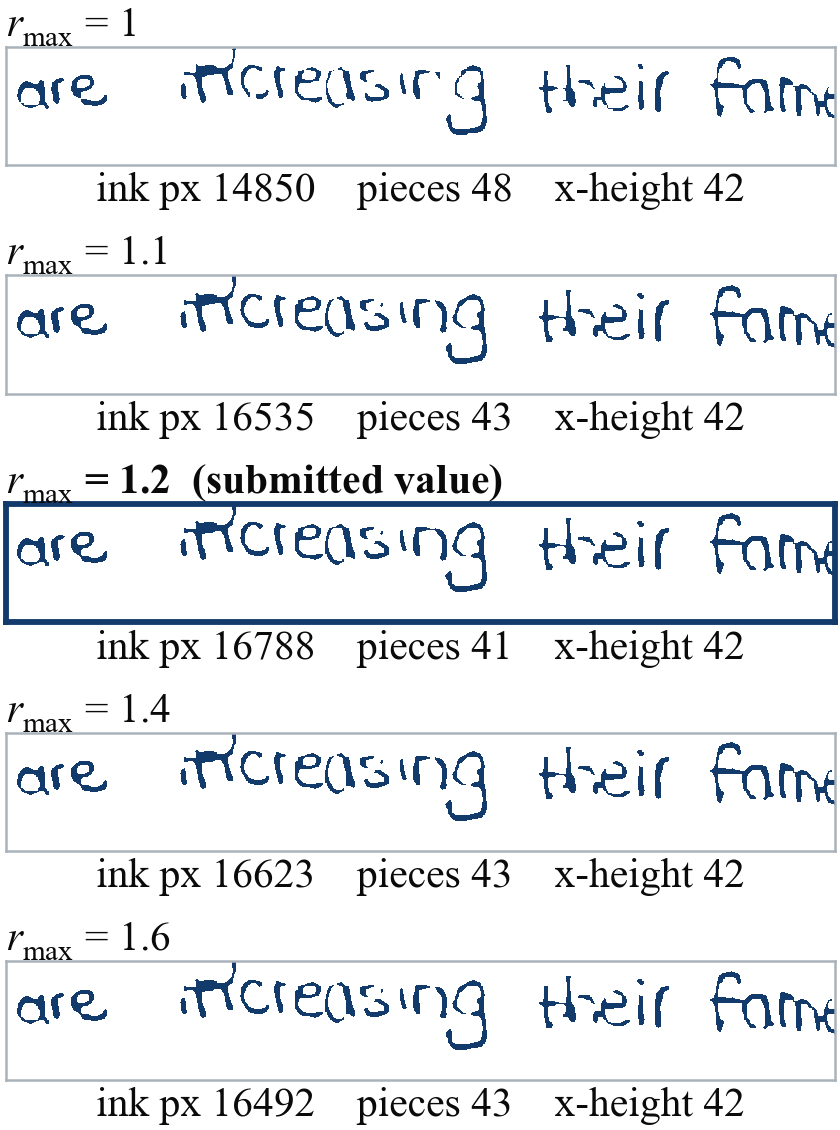
\includegraphics[width=\linewidth]{../figures/otsu_hi.png}

\caption{Upper edge of the histogram Otsu is built on, for a ratio image. Each panel is the same input processed by the submitted code with only $r_{\max}$ changed; the panel outlined in dark blue is the submitted value.}

\label{fig:otsu-hi}

\end{figure}

\begin{figure}[htbp]

\centering

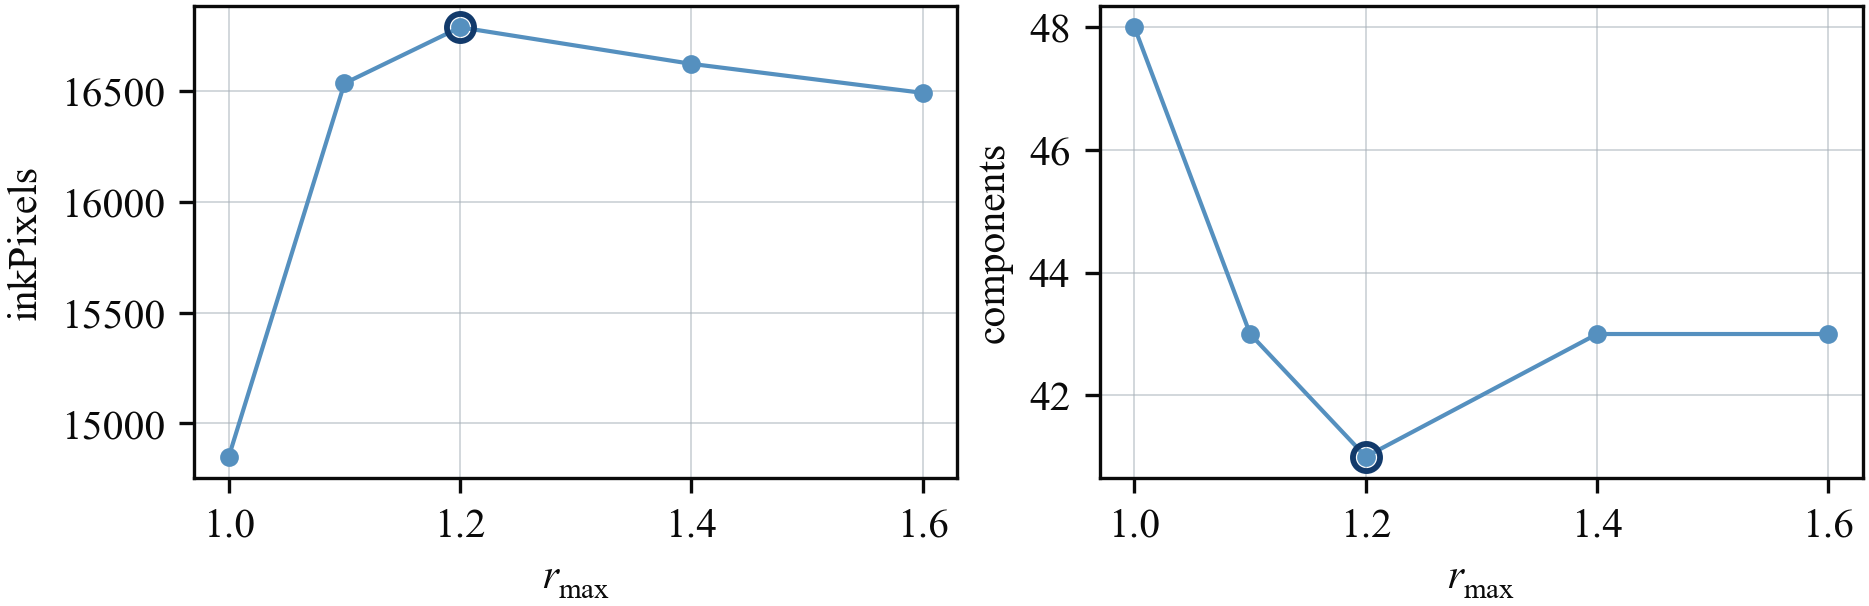
\includegraphics[width=\linewidth]{../figures/otsu_hi_trend.png}

\caption{Upper edge of the histogram Otsu is built on, for a ratio image: measured quantities against the swept value. The circled point is the submitted value.}

\end{figure}

\begin{table}[htbp]
\centering
\small
\caption{Upper edge of the histogram Otsu is built on, for a ratio image: measured effect of each swept value. The submitted value is in bold.}
\begin{tabular}{lrrr}
\toprule
\$r\_\{\textbackslash\{\}max\}\$ & \textsf{inkPixels} & \textsf{components} & \textsf{xh} \\
\midrule
1 & 14850 & 48 & 42 \\
1.1 & 16535 & 43 & 42 \\
\bfseries 1.2 & \bfseries 16788 & \bfseries 41 & \bfseries 42 \\
1.4 & 16623 & 43 & 42 \\
1.6 & 16492 & 43 & 42 \\
\bottomrule
\end{tabular}
\end{table}

\section{Line binarisation}

\subsection{Width below which a run of ink counts as thin, for printed-rule removal}

\label{coef:binarize-thin}

\begin{description}[leftmargin=5.2em,style=sameline]

\item[Symbol] $w_{\text{thin}}$

\item[Value] \texttt{0.12}

\item[Source] \texttt{segment.py}, \texttt{BinarizeLine}

\item[Swept] \texttt{0.06}, \texttt{0.09}, \texttt{0.12}, \texttt{0.18}, \texttt{0.24}

\end{description}

\paragraph{Basis}

Removing long thin runs is the standard morphological test for printed rules and table lines in document analysis \cite{haralick1987}; the ruling on a form is the structure Shafait \textit{et al.} \cite{shafait2008} evaluate layout methods against.

\paragraph{Why this value}

A printed rule is the one mark on these pages that is simultaneously very long horizontally and very short vertically. The test is the conjunction of both, so the thinness limit only has to separate a printed line from a pen stroke. Measured pen strokes on the photographed pages run $4$--$9$ px thick at a crop height of $156$ px, that is $0.026$--$0.058\,h$; the printed rule is $1$--$3$ px. $0.12\,h$ sits above the rule and below the thinnest real stroke, with the floor $\max(3,\cdot)$ protecting small crops.

\paragraph{What the coefficient does}

$w_{\text{thin}}$ is a fraction of the crop height $h$, so it scales with how big the writing was photographed. Too small and a thick printed rule survives; too large and a horizontal pen stroke, such as the bar of a \texttt{t} or the body of an \texttt{e}, is deleted as structure.

\paragraph{Alternatives considered}

A Hough transform for straight lines \cite{duda1972}, which finds rules at any angle but costs an accumulator per crop and needs its own peak threshold, or projection-profile rule detection, which is what \texttt{train.py} uses on whole pages in \texttt{FindRuleLineClusters}.

\paragraph{Worked example}

At $h=156$ px, $0.12\,h = 18.7 \to 18$ px, and the length test is $\max(24,\lfloor 1.1h \rfloor) = 171$ px. A mark is deleted only if it is at least $171$ px long and at most $18$ px tall.

\paragraph{What the sweep actually showed}

\textbf{This sweep showed no effect at all}: ink pixels, component count, band and slant are identical at all five values. The reason is structural, not a failure of the sweep. By the time \texttt{BinarizeLine} sees a crop, \texttt{RemovePrintedStructure} has already deleted the page's ruling at page scale, so there is no printed rule left in the crop for the line-level test to find. On this input the coefficient is dead code. That does not make it wrong to have: it is the guard for a crop that reaches the binariser without having been through the page-level removal, which is the path \texttt{style.py} takes when it binarises a crop directly. Exercising it properly needs a crop that still contains ruling, which this probe does not provide.

\begin{figure}[htbp]

\centering

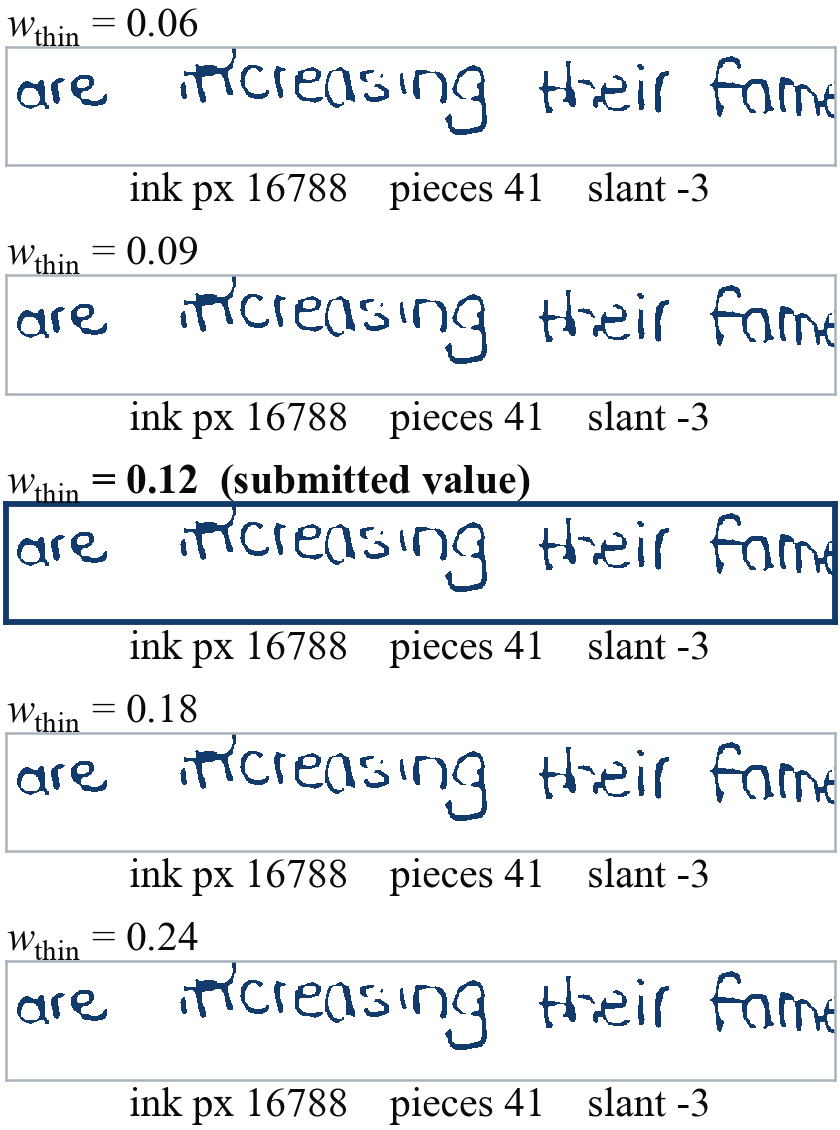
\includegraphics[width=\linewidth]{../figures/binarize_thin.png}

\caption{Width below which a run of ink counts as thin, for printed-rule removal. Each panel is the same input processed by the submitted code with only $w_{\text{thin}}$ changed; the panel outlined in dark blue is the submitted value.}

\label{fig:binarize-thin}

\end{figure}

\begin{figure}[htbp]

\centering

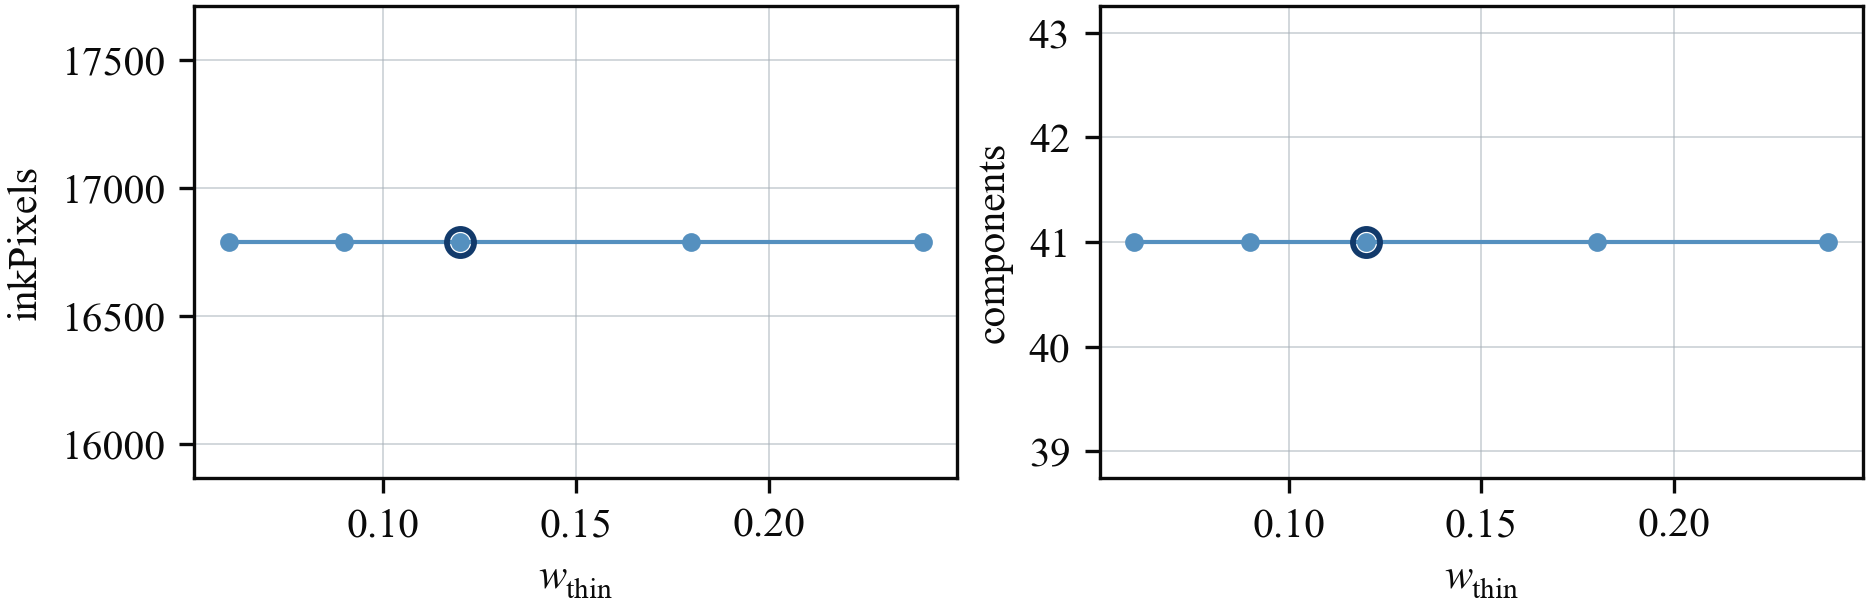
\includegraphics[width=\linewidth]{../figures/binarize_thin_trend.png}

\caption{Width below which a run of ink counts as thin, for printed-rule removal: measured quantities against the swept value. The circled point is the submitted value.}

\end{figure}

\begin{table}[htbp]
\centering
\small
\caption{Width below which a run of ink counts as thin, for printed-rule removal: measured effect of each swept value. The submitted value is in bold.}
\begin{tabular}{lrrr}
\toprule
\$w\_\{\textbackslash\{\}text\{thin\}\}\$ & \textsf{inkPixels} & \textsf{components} & \textsf{slantDeg} \\
\midrule
0.06 & 16788 & 41 & -3 \\
0.09 & 16788 & 41 & -3 \\
\bfseries 0.12 & \bfseries 16788 & \bfseries 41 & \bfseries -3 \\
0.18 & 16788 & 41 & -3 \\
0.24 & 16788 & 41 & -3 \\
\bottomrule
\end{tabular}
\end{table}

\subsection{Length above which a run of ink counts as a printed rule}

\label{coef:binarize-rulelen}

\begin{description}[leftmargin=5.2em,style=sameline]

\item[Symbol] $L_{\text{rule}}$

\item[Value] \texttt{1.1}

\item[Source] \texttt{segment.py}, \texttt{BinarizeLine}

\item[Swept] \texttt{0.6}, \texttt{0.85}, \texttt{1.1}, \texttt{1.5}, \texttt{2.0}

\end{description}

\paragraph{Basis}

Same basis as the thinness test: long-run structure removal \cite{haralick1987,shafait2008}.

\paragraph{Why this value}

The rule on a ruled page runs the full width of the writing area, which is many times the height of one line of writing. Expressing the limit in crop heights makes it scale-free: a rule is longer than the line is tall, a pen stroke is not. $1.1\,h$ is just over one line height, which no single handwritten stroke on these pages reaches horizontally while staying under $0.12\,h$ thick.

\paragraph{What the coefficient does}

Lowering $L_{\text{rule}}$ makes the test fire on ordinary writing, because a joined cursive word can be several line heights long: only the thinness test then stands between the writing and deletion. Raising it lets a short rule segment, or a rule broken by the writing crossing it, survive into the mask.

\paragraph{Alternatives considered}

An absolute pixel length, which breaks as soon as the page is photographed at a different distance, or connected-component aspect ratio, which a long joined word also satisfies.

\paragraph{Worked example}

At $h=156$ px the limit is $171$ px, which is $11\%$ of the $2170$ px crop width, so a rule has to cross about a ninth of the writing area before it is removed.

\paragraph{What the sweep actually showed}

As with the thinness limit, \textbf{no effect was measured}: the page-level structure removal has already taken the ruling out before the crop is built, so the length test never fires on this input. The same caveat applies: the sweep bounds the coefficient's effect on this path at zero, and says nothing about the direct-binarisation path.

\begin{figure}[htbp]

\centering

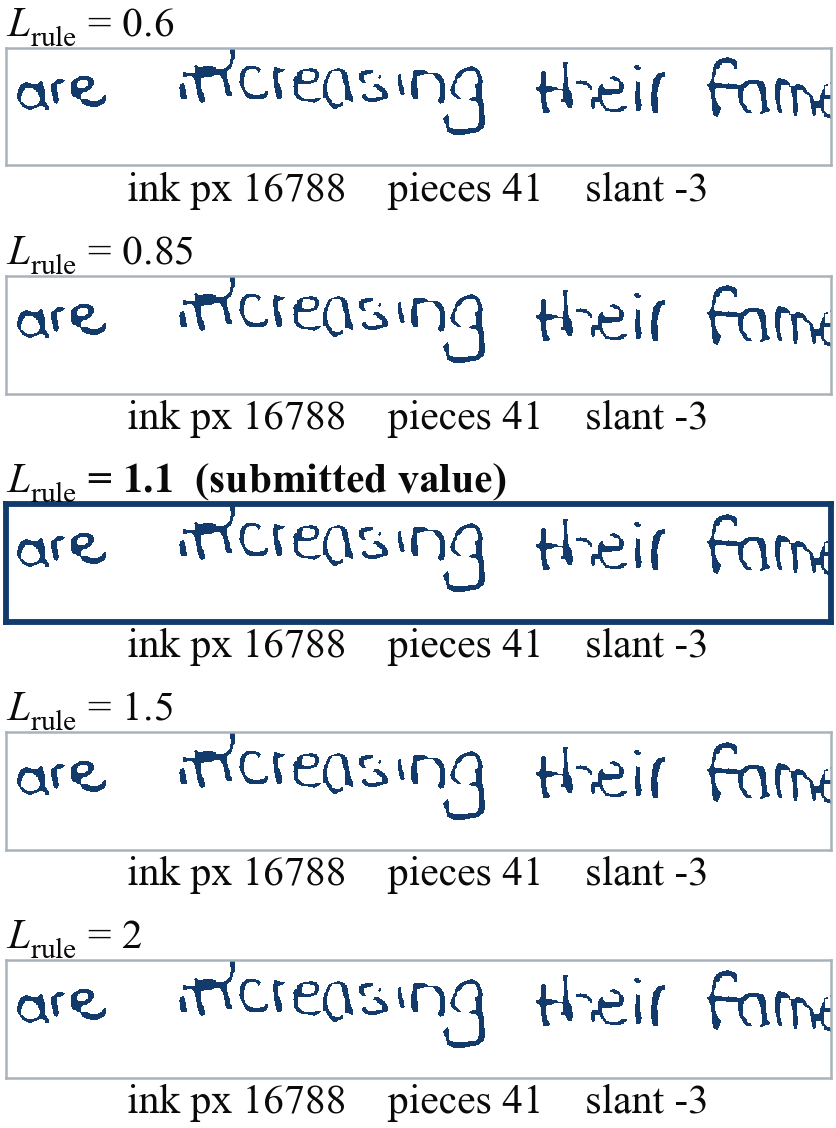
\includegraphics[width=\linewidth]{../figures/binarize_rulelen.png}

\caption{Length above which a run of ink counts as a printed rule. Each panel is the same input processed by the submitted code with only $L_{\text{rule}}$ changed; the panel outlined in dark blue is the submitted value.}

\label{fig:binarize-rulelen}

\end{figure}

\begin{figure}[htbp]

\centering

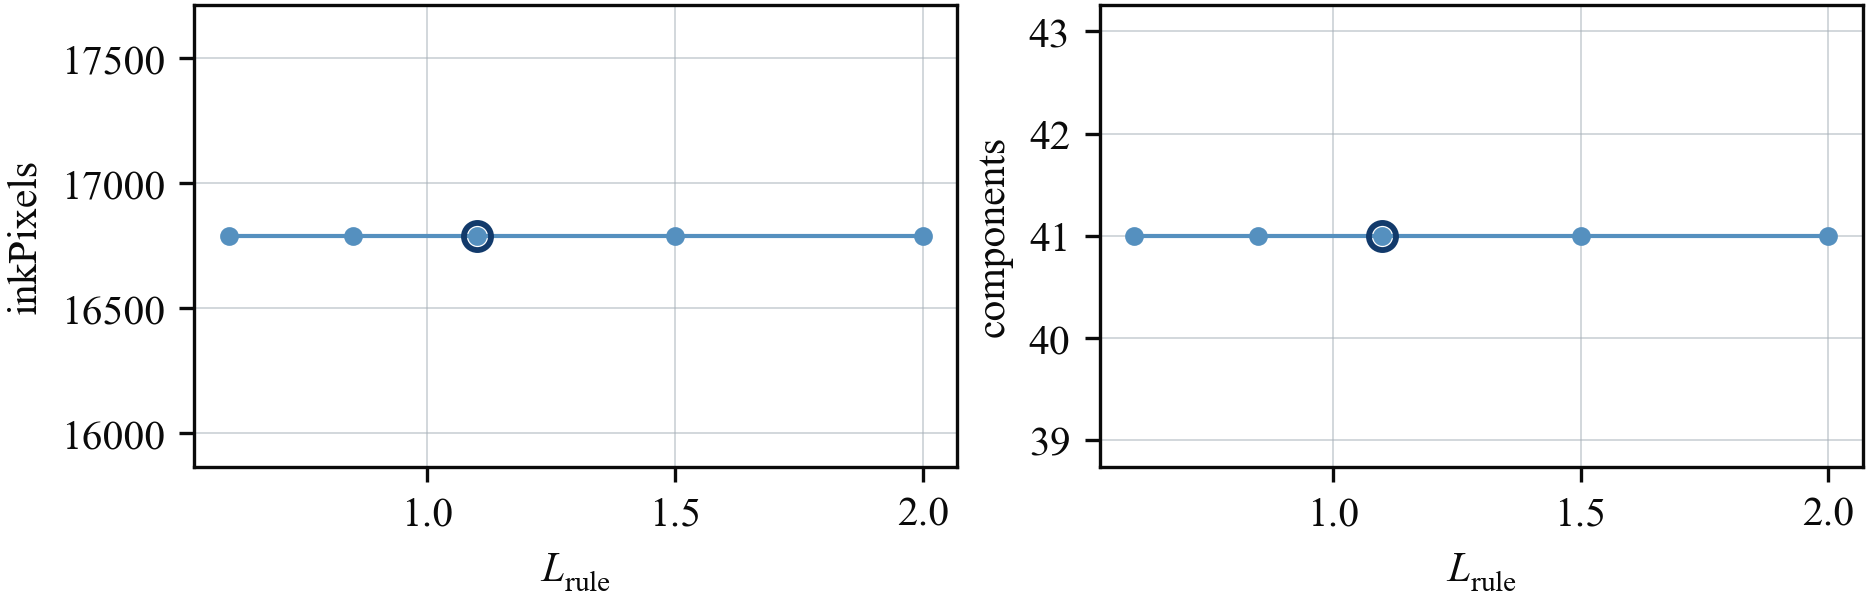
\includegraphics[width=\linewidth]{../figures/binarize_rulelen_trend.png}

\caption{Length above which a run of ink counts as a printed rule: measured quantities against the swept value. The circled point is the submitted value.}

\end{figure}

\begin{table}[htbp]
\centering
\small
\caption{Length above which a run of ink counts as a printed rule: measured effect of each swept value. The submitted value is in bold.}
\begin{tabular}{lrrr}
\toprule
\$L\_\{\textbackslash\{\}text\{rule\}\}\$ & \textsf{inkPixels} & \textsf{components} & \textsf{slantDeg} \\
\midrule
0.6 & 16788 & 41 & -3 \\
0.85 & 16788 & 41 & -3 \\
\bfseries 1.1 & \bfseries 16788 & \bfseries 41 & \bfseries -3 \\
1.5 & 16788 & 41 & -3 \\
2 & 16788 & 41 & -3 \\
\bottomrule
\end{tabular}
\end{table}

\subsection{Closing radius that bridges pinholes in a stroke}

\label{coef:binarize-close}

\begin{description}[leftmargin=5.2em,style=sameline]

\item[Symbol] $k_{\text{close}}$

\item[Value] \texttt{0.045}

\item[Source] \texttt{segment.py}, \texttt{BinarizeLine}

\item[Swept] \texttt{0.0}, \texttt{0.02}, \texttt{0.045}, \texttt{0.08}, \texttt{0.12}

\end{description}

\paragraph{Basis}

Morphological closing, dilation followed by erosion by the same element, is the classical repair for small holes and gaps and does not grow the shape overall \cite{haralick1987}.

\paragraph{Why this value}

A ballpoint on ordinary paper skips, so a single stroke binarises into a chain of blobs. Those breaks matter twice over: they split one component into several, and they put spurious endpoints into the skeleton, which the tracer then follows as separate strokes. The radius has to close a skip without fattening the stroke, so it is tied to the crop height and then hard-clipped to $2$--$4$ px: the clip, not the fraction, is what finally bounds the damage.

\paragraph{What the coefficient does}

Because of the $\mathrm{clip}(\cdot,2,4)$ the coefficient only has an effect between $h=44$ and $h=89$ px; outside that range the clip decides. On the probe crop ($h=156$) every value from $0.02$ upward gives $k=4$, which is why the sweep includes $0$: that is the only setting that changes the picture, and it shows what closing is buying.

\paragraph{Alternatives considered}

Not closing at all and letting the tracer rejoin the pieces at junctions, which \texttt{\_JoinAtJunctions} does anyway; or a larger closing, which merges adjacent letters and destroys the character boundaries the glyph cutter depends on.

\paragraph{Worked example}

At $h=156$ px, $0.045\,h = 7.0$, clipped to $4$, so a $4\times4$ closing is applied: gaps up to about $4$ px of white inside a stroke are filled.

\paragraph{What the sweep actually showed}

Two distinct outcomes appear across five values, not five, and the reason is the quantisation described above. At $h = 156$ px the kernel is $k = \mathrm{clip}(\mathrm{round}(c\,h),2,4)$ and the dilation radius is $k//2$: $c = 0$ gives $k = 2$ and $c = 0.02$ gives $k = 3$, both of which are radius~$1$, while $c \ge 0.045$ gives $k = 4$, radius~$2$. So the sweep really compares radius~$1$ with radius~$2$, and the difference is clear: radius~$1$ leaves $16\,401$ ink pixels in $47$ components and radius~$2$ leaves $16\,788$ in $41$. Closing at the submitted value merges six broken pieces back into their strokes and adds $387$ pixels of ink, which is what it is for.

\begin{figure}[htbp]

\centering

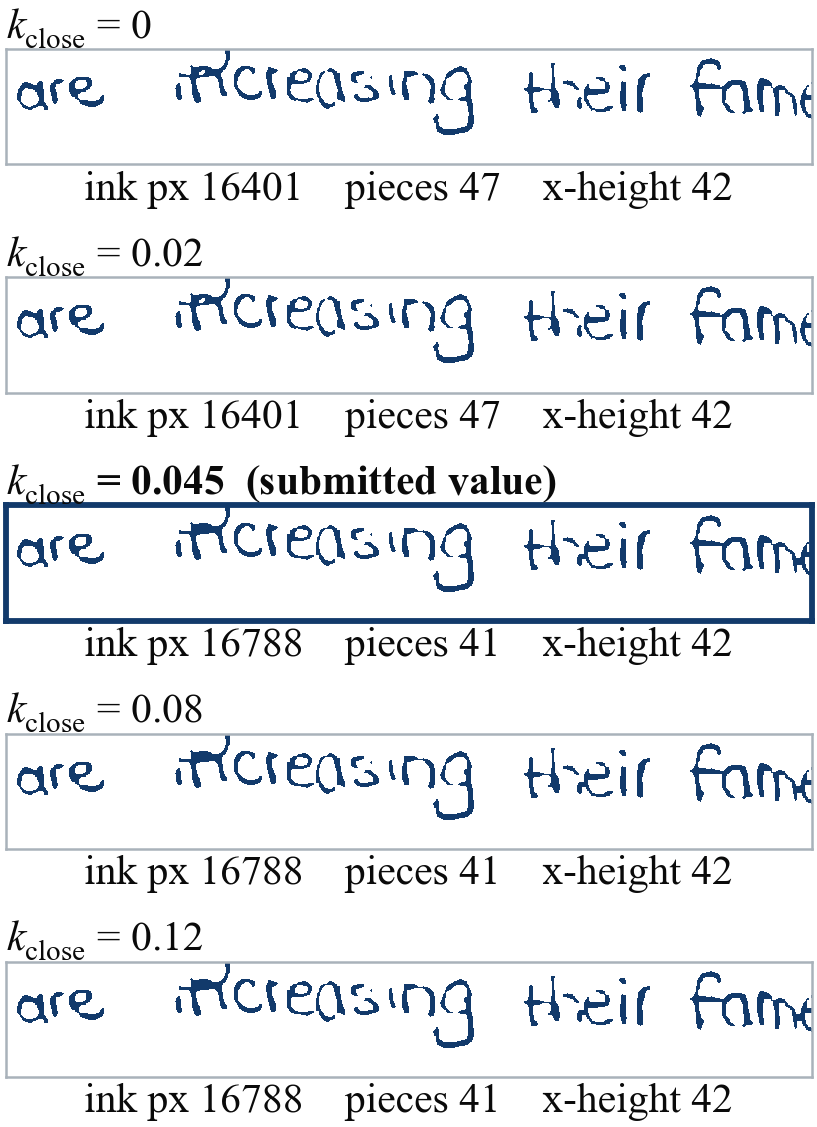
\includegraphics[width=\linewidth]{../figures/binarize_close.png}

\caption{Closing radius that bridges pinholes in a stroke. Each panel is the same input processed by the submitted code with only $k_{\text{close}}$ changed; the panel outlined in dark blue is the submitted value.}

\label{fig:binarize-close}

\end{figure}

\begin{figure}[htbp]

\centering

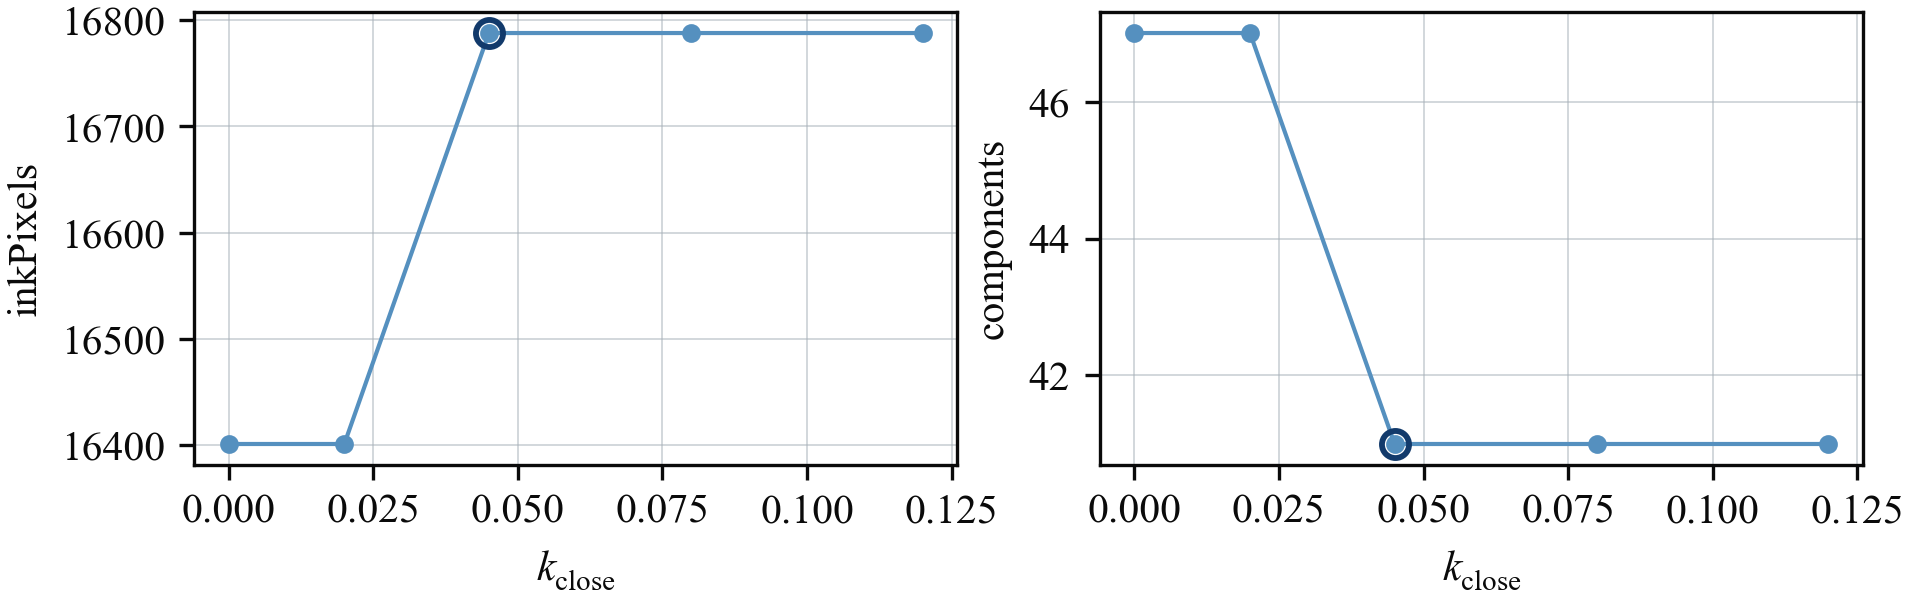
\includegraphics[width=\linewidth]{../figures/binarize_close_trend.png}

\caption{Closing radius that bridges pinholes in a stroke: measured quantities against the swept value. The circled point is the submitted value.}

\end{figure}

\begin{table}[htbp]
\centering
\small
\caption{Closing radius that bridges pinholes in a stroke: measured effect of each swept value. The submitted value is in bold.}
\begin{tabular}{lrrr}
\toprule
\$k\_\{\textbackslash\{\}text\{close\}\}\$ & \textsf{inkPixels} & \textsf{components} & \textsf{xh} \\
\midrule
0 & 16401 & 47 & 42 \\
0.02 & 16401 & 47 & 42 \\
\bfseries 0.045 & \bfseries 16788 & \bfseries 41 & \bfseries 42 \\
0.08 & 16788 & 41 & 42 \\
0.12 & 16788 & 41 & 42 \\
\bottomrule
\end{tabular}
\end{table}

\subsection{Smallest component kept in a line mask}

\label{coef:speck-area}

\begin{description}[leftmargin=5.2em,style=sameline]

\item[Symbol] $A_{\min}$

\item[Value] \texttt{6}

\item[Source] \texttt{segment.py}, \texttt{BinarizeLine}

\item[Swept] \texttt{1}, \texttt{3}, \texttt{6}, \texttt{12}, \texttt{24}

\end{description}

\paragraph{Basis}

Area opening, discarding components below a size, is the standard speck filter after thresholding \cite{haralick1987}; components are labelled by the two-pass union-find of Rosenfeld and Pfaltz \cite{rosenfeld1966} with path compression after Tarjan \cite{tarjan1975}.

\paragraph{Why this value}

Thresholding a photograph leaves single-pixel noise from sensor grain and paper texture. The smallest mark that must survive is the dot of an \texttt{i} or a full stop, which on these crops is $20$--$60$ px. $A_{\min}=6$ is an order of magnitude below the smallest real mark and an order above single-pixel grain, so it is deliberately not a tuned value: it sits in the gap.

\paragraph{What the coefficient does}

Raising it eventually eats punctuation and \texttt{i} dots, which the glyph cutter then has to recover separately in \texttt{ExtractLineGlyphs}. Lowering it to $1$ keeps every speck, which inflates the component count the ownership stage has to reason about.

\paragraph{Alternatives considered}

A median or morphological opening before labelling, which also rounds the stroke ends, or keeping everything and letting the later size tests in \texttt{\_BandOwnership} reject it, which is what happens for anything above $6$ px anyway.

\paragraph{Worked example}

On the probe crop the mask holds $41$ components at $A_{\min}=6$; the sweep records how that count moves with the limit.

\paragraph{What the sweep actually showed}

The component count falls monotonically, $46$, $44$, $41$, $40$, $38$, while the ink pixel count barely moves, $16\,802$ down to $16\,743$. That is the signature of a speck filter working as intended: it is removing many tiny pieces and almost no ink. Between $A_{\min} = 1$ and the submitted $6$, five components disappear for the loss of $14$ pixels. Raising it to $24$ removes three more components and $45$ more pixels, and at that point it is beginning to reach marks large enough to be punctuation.

\begin{figure}[htbp]

\centering

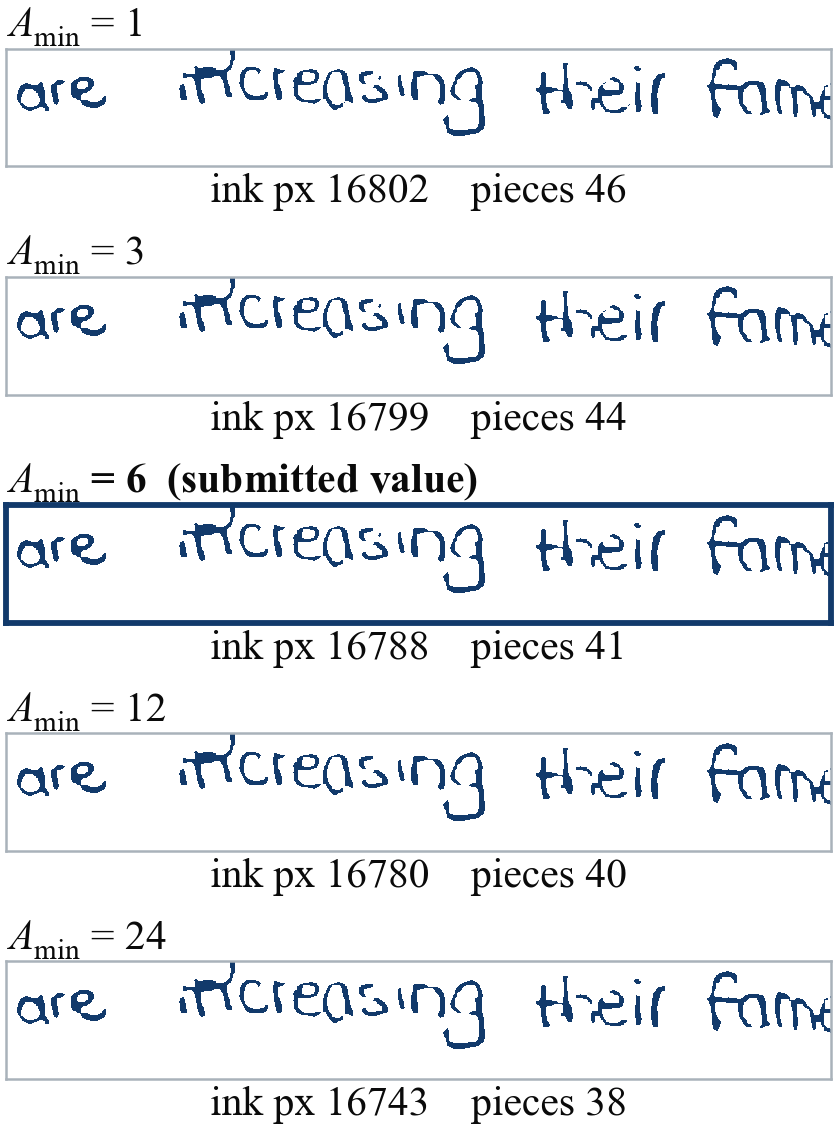
\includegraphics[width=\linewidth]{../figures/speck_area.png}

\caption{Smallest component kept in a line mask. Each panel is the same input processed by the submitted code with only $A_{\min}$ changed; the panel outlined in dark blue is the submitted value.}

\label{fig:speck-area}

\end{figure}

\begin{figure}[htbp]

\centering

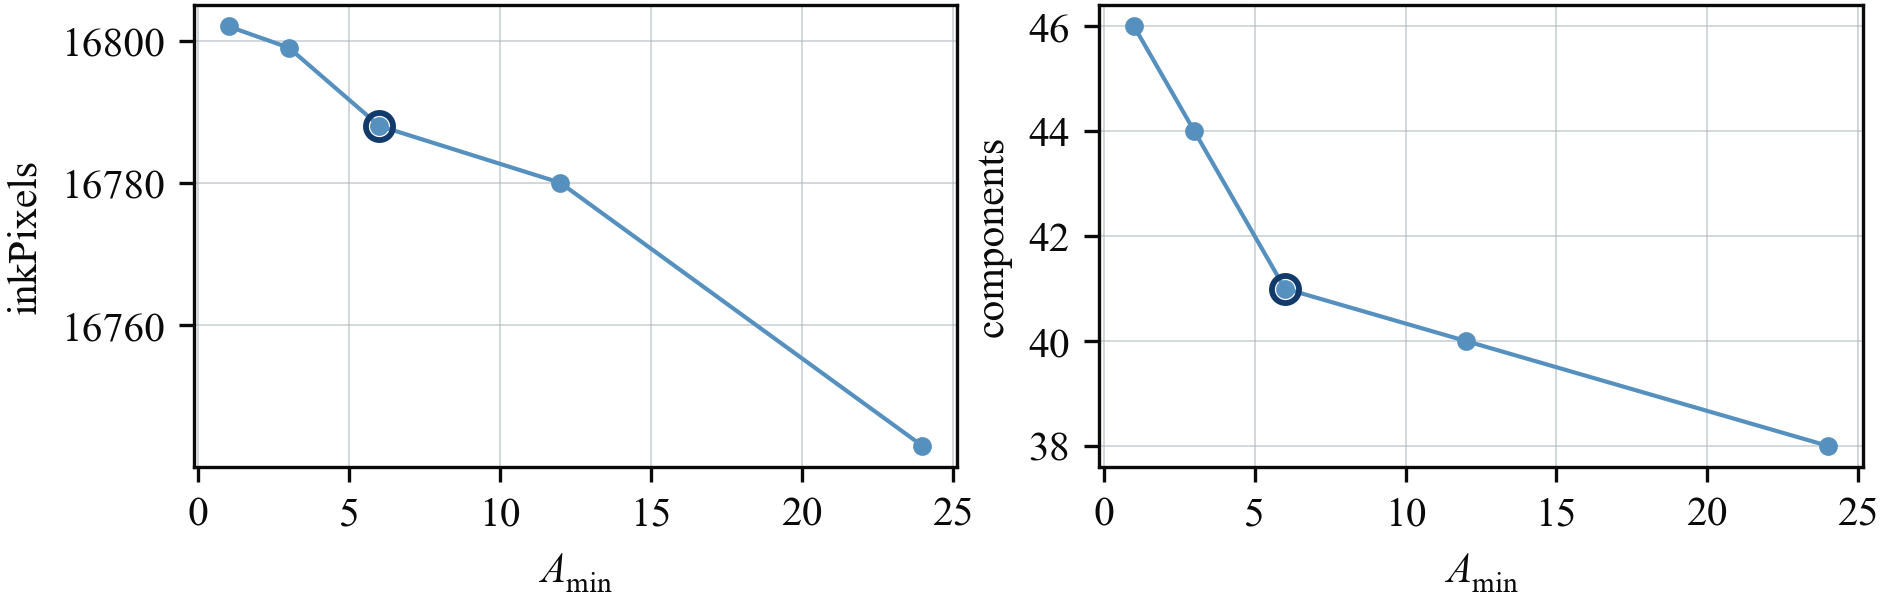
\includegraphics[width=\linewidth]{../figures/speck_area_trend.png}

\caption{Smallest component kept in a line mask: measured quantities against the swept value. The circled point is the submitted value.}

\end{figure}

\begin{table}[htbp]
\centering
\small
\caption{Smallest component kept in a line mask: measured effect of each swept value. The submitted value is in bold.}
\begin{tabular}{lrr}
\toprule
\$A\_\{\textbackslash\{\}min\}\$ & \textsf{inkPixels} & \textsf{components} \\
\midrule
1 & 16802 & 46 \\
3 & 16799 & 44 \\
\bfseries 6 & \bfseries 16788 & \bfseries 41 \\
12 & 16780 & 40 \\
24 & 16743 & 38 \\
\bottomrule
\end{tabular}
\end{table}

\section{Line geometry}

\subsection{Profile height defining the x-height band}

\label{coef:core-band-frac}

\begin{description}[leftmargin=5.2em,style=sameline]

\item[Symbol] $\tau_{\text{band}}$

\item[Value] \texttt{0.45}

\item[Source] \texttt{segment.py}, \texttt{CoreBand}

\item[Swept] \texttt{0.25}, \texttt{0.35}, \texttt{0.45}, \texttt{0.6}, \texttt{0.75}

\end{description}

\paragraph{Basis}

The horizontal projection profile of a text line peaks across the x-height body and falls away over the ascender and descender zones; this is the basis of profile-based line and zone finding \cite{likforman2007}, and the same profile drives the IAM baseline work \cite{marti2002}.

\paragraph{Why this value}

Every shape in a style profile is stored in x-heights, so the x-height is the one length the whole synthesis side depends on. It is measured as the band of rows carrying at least $\tau_{\text{band}}$ of the peak ink-per-row. The body of the writing contributes nearly every row of ink; ascenders and descenders contribute only the few columns that have them. The profile therefore has a plateau and a skirt, and $\tau_{\text{band}}$ has to cut the skirt. At $0.45$ the cut is roughly half the plateau height, which is above the ascender skirt on all eleven writers and below the plateau edge on all of them.

\paragraph{What the coefficient does}

This coefficient directly scales every stored glyph. If $\tau_{\text{band}}$ is too low the band swallows the ascender zone, the measured x-height grows, and every glyph is stored too small, so the writing is later drawn too large for its ruling. Too high and the band collapses onto the few darkest rows. The guard \texttt{base-top>=3} rejects a collapsed band outright rather than returning a bad number.

\paragraph{Alternatives considered}

Fitting four baselines explicitly, as Vinciarelli and Luettin do \cite{vinciarelli2001}, which is more faithful but needs its own model fit per line; or taking the median component height, which \texttt{\_LetterHeight} does for line pitch but which mixes ascenders into the estimate.

\paragraph{Worked example}

On the probe crop the band is rows $36$--$78$, giving $x_h = 42$ px at a crop height of $156$ px, so the x-height is $27\%$ of the crop and the ascender and descender zones take the rest.

\paragraph{What the sweep actually showed}

The measured x-height moves by a factor of $3.5$ across the sweep: $59$, $54$, $42$, $24$, $17$ px, while the ink mask itself is byte-for-byte identical at every value, since this coefficient only reads the profile. The figure shows the consequence directly: at $0.25$ the band has swallowed the ascender zone and at $0.75$ it has collapsed onto the densest rows of the body. The submitted value is the only one of the five whose band visibly hugs the x-height body, which is what the measurement is supposed to mean. Because every stored glyph is divided by this number, the $3.5\times$ spread here is a $3.5\times$ spread in the stored size of every letter.

\begin{figure}[htbp]

\centering

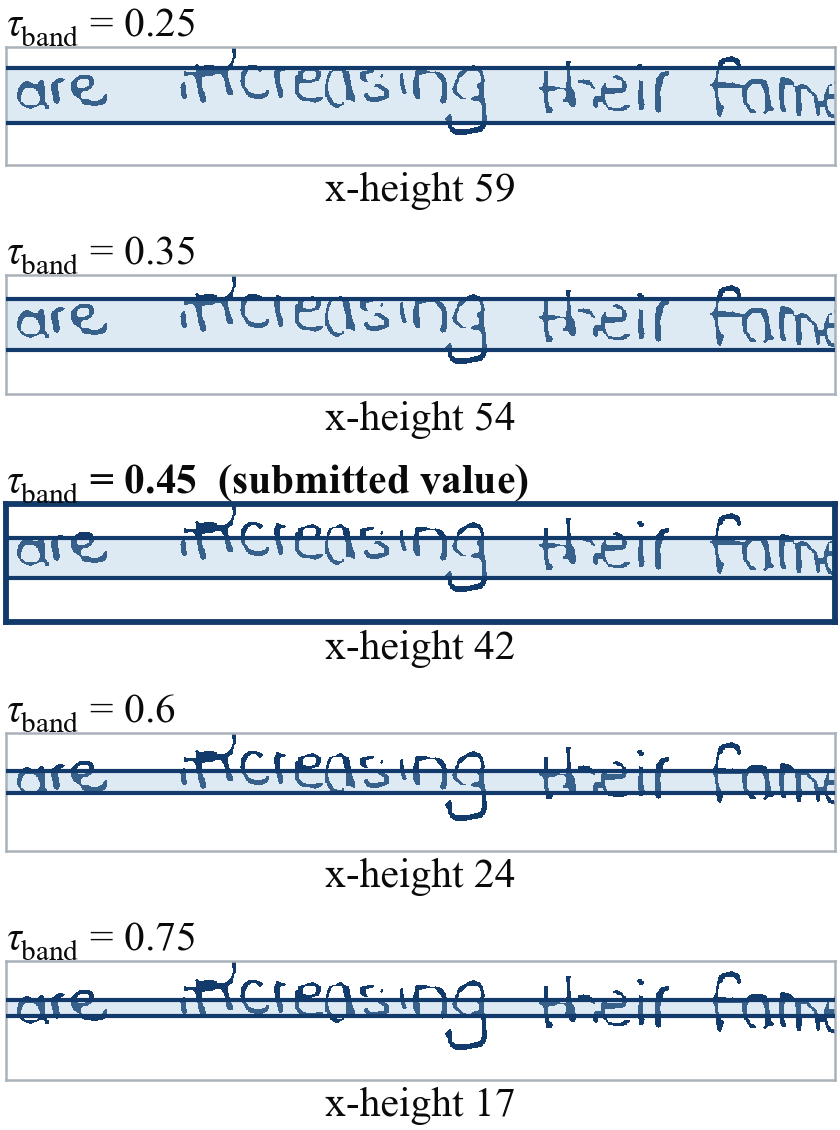
\includegraphics[width=\linewidth]{../figures/core_band_frac.png}

\caption{Profile height defining the x-height band. Each panel is the same input processed by the submitted code with only $\tau_{\text{band}}$ changed; the panel outlined in dark blue is the submitted value.}

\label{fig:core-band-frac}

\end{figure}

\begin{figure}[htbp]

\centering

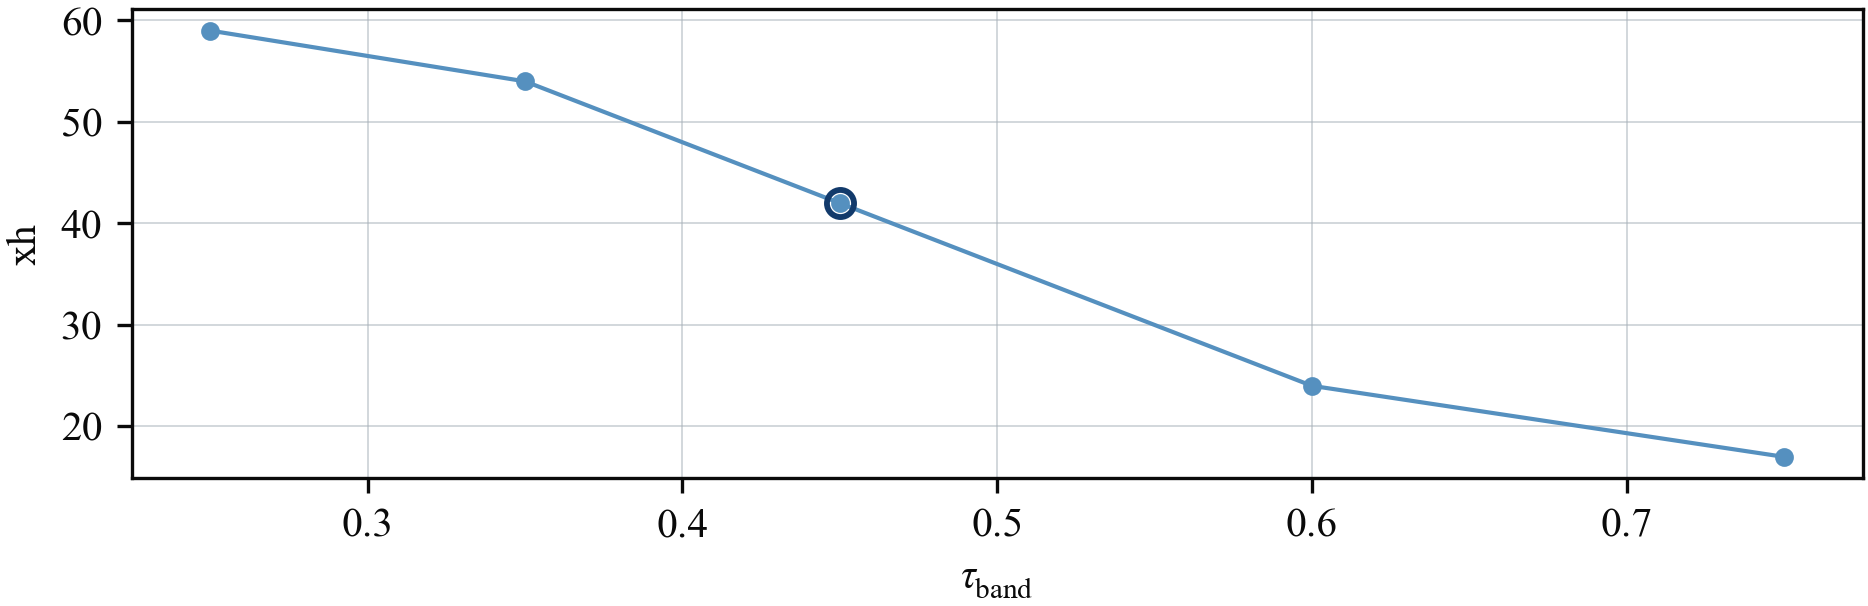
\includegraphics[width=\linewidth]{../figures/core_band_frac_trend.png}

\caption{Profile height defining the x-height band: measured quantities against the swept value. The circled point is the submitted value.}

\end{figure}

\begin{table}[htbp]
\centering
\small
\caption{Profile height defining the x-height band: measured effect of each swept value. The submitted value is in bold.}
\begin{tabular}{lrr}
\toprule
\$\textbackslash\{\}tau\_\{\textbackslash\{\}text\{band\}\}\$ & \textsf{xh} & \textsf{coreBand} \\
\midrule
0.25 & 59 & [22, 81] \\
0.35 & 54 & [25, 79] \\
\bfseries 0.45 & \bfseries 42 & \bfseries [36, 78] \\
0.6 & 24 & [40, 64] \\
0.75 & 17 & [41, 58] \\
\bottomrule
\end{tabular}
\end{table}

\section{Illumination normalisation}

\subsection{Local background radius for the ink mask}

\label{coef:inkmask-bgradius}

\begin{description}[leftmargin=5.2em,style=sameline]

\item[Symbol] $r_{\text{bg}}$

\item[Value] \texttt{41}

\item[Source] \texttt{segment.py}, \texttt{InkMask}

\item[Swept] \texttt{15}, \texttt{25}, \texttt{41}, \texttt{70}, \texttt{120}

\end{description}

\paragraph{Basis}

Dividing by a local mean computed from an integral image is Bradley and Roth's adaptive threshold \cite{bradley2007}; the constant-time rectangle sum it needs is Crow's summed-area table \cite{crow1984}.

\paragraph{Why this value}

A phone photograph of a page is unevenly lit, so no single grey level separates ink from paper across the whole sheet. Each pixel is therefore compared with the mean of a window around it. The window has to be much larger than a stroke, or it averages the ink into its own background and the stroke centre is lost, and much smaller than the illumination gradient, or it stops tracking the shading. Tying it to $H/41$ makes it track how large the writing was photographed rather than the sensor resolution, and the $\mathrm{clip}(8,40)$ keeps it inside the range where both conditions hold.

\paragraph{What the coefficient does}

At $H/41$ the window is about three x-heights across, so a stroke occupies a few per cent of it. The clip means the coefficient only bites for page heights between $328$ and $1640$ px at half resolution; the probe page is $1632$ px tall at half size, so it sits at the very top of that range and the sweep moves the radius over most of its useful span.

\paragraph{Alternatives considered}

Sauvola's local mean and standard deviation \cite{sauvola2000} or Niblack's \cite{niblack1986}, both of which add a sensitivity constant; a morphological top-hat, which needs a structuring element of the same scale; or global Otsu alone, which fails outright on a shadowed corner.

\paragraph{Worked example}

The probe page is $3264$ px tall, halved to $1632$, so $1632/41 = 39.8 \to 40$, exactly at the clip. The window is $81\times81$ px against an x-height of about $21$ px at half resolution, that is $3.9$ x-heights wide.

\paragraph{What the sweep actually showed}

The first three values are identical, because the $\mathrm{clip}(8,40)$ holds the radius at $40$ px for all of them on a page this size: $1632/41 = 39.8$, $1632/25 = 65$ and $1632/15 = 109$ all clip to $40$. The sweep therefore only moves the radius downward, at $70$ and $120$, where it becomes $23$ and $14$ px. The effect is immediate: straight-structure removal jumps from $1\,988$ pixels to $6\,114$ and $6\,808$, and the estimated line pitch shifts from $51$ to $50$ px. A background window that small starts to average the stroke into its own background, the mask degrades, and the long-run tests then fire on parts of the writing. Reading accuracy falls from $0.982$ to $0.975$. The submitted value is at the top of its clip and is the safe end.

\begin{figure}[htbp]

\centering

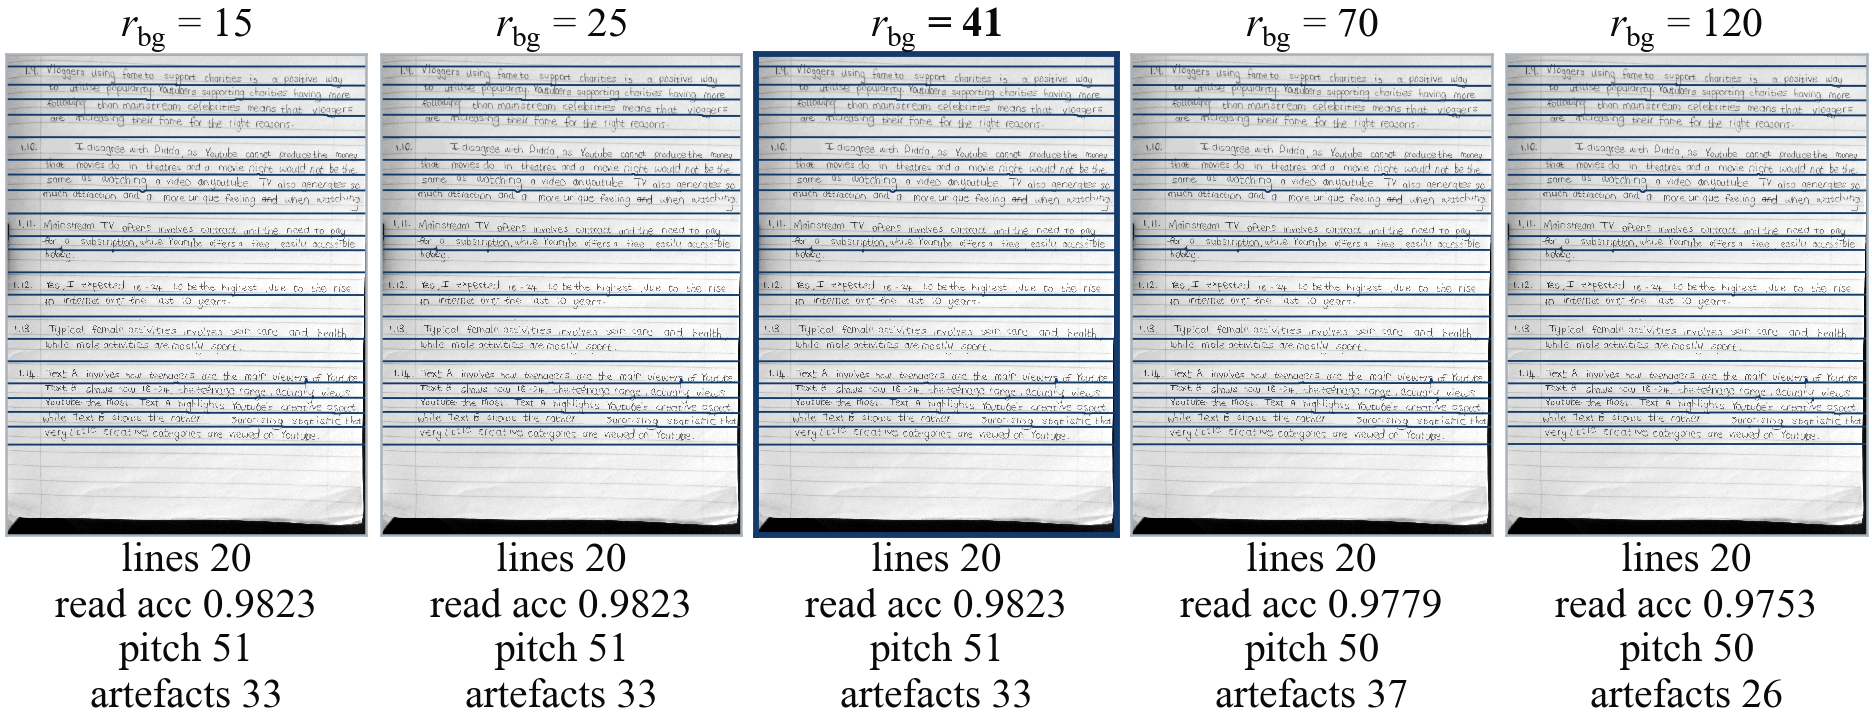
\includegraphics[width=\linewidth]{../figures/inkmask_bgradius.png}

\caption{Local background radius for the ink mask. Each panel is the same input processed by the submitted code with only $r_{\text{bg}}$ changed; the panel outlined in dark blue is the submitted value.}

\label{fig:inkmask-bgradius}

\end{figure}

\begin{figure}[htbp]

\centering

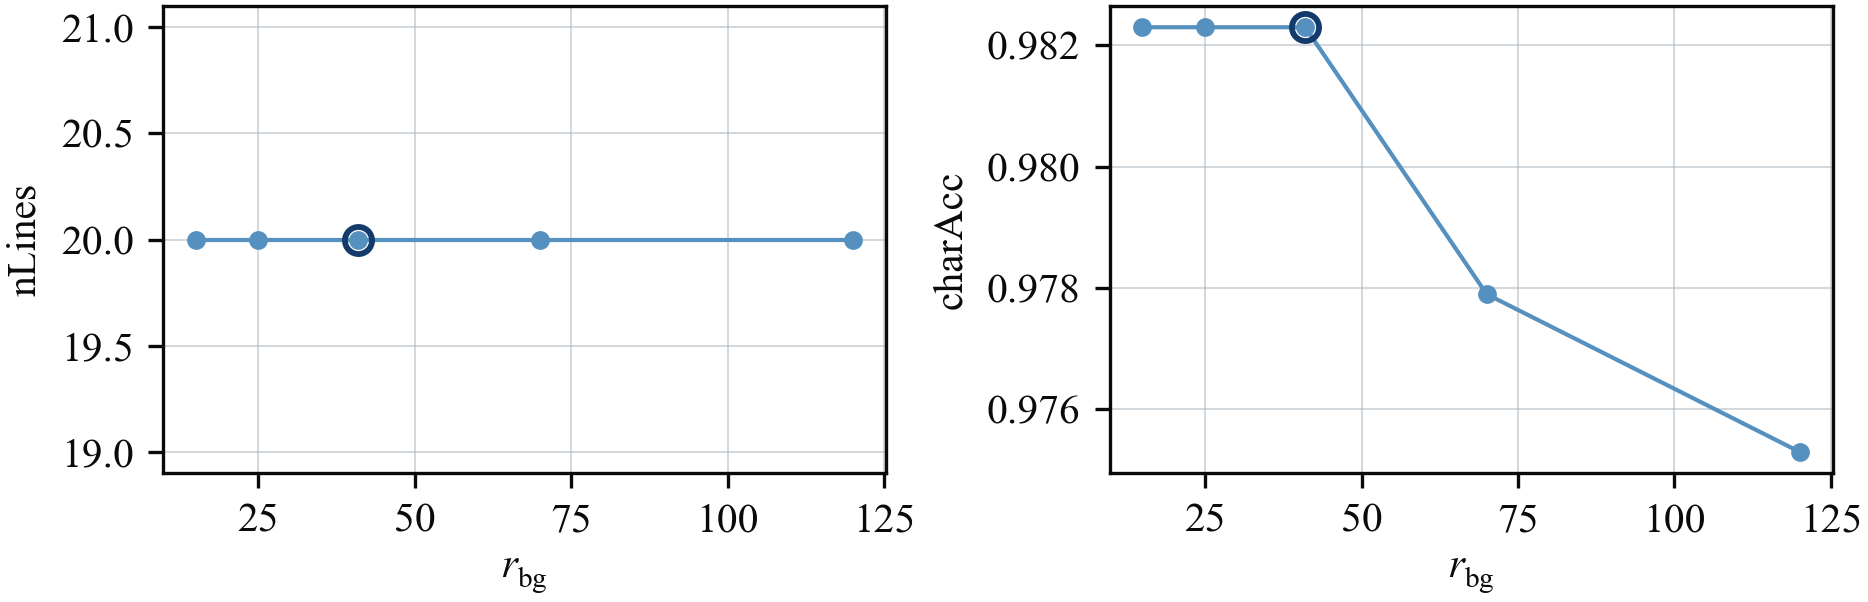
\includegraphics[width=\linewidth]{../figures/inkmask_bgradius_trend.png}

\caption{Local background radius for the ink mask: measured quantities against the swept value. The circled point is the submitted value.}

\end{figure}

\begin{table}[htbp]
\centering
\small
\caption{Local background radius for the ink mask: measured effect of each swept value. The submitted value is in bold.}
\begin{tabular}{lrrrr}
\toprule
\$r\_\{\textbackslash\{\}text\{bg\}\}\$ & \textsf{nLines} & \textsf{charAcc} & \textsf{pitch} & \textsf{artifactPieces} \\
\midrule
15 & 20 & 0.9823 & 51 & 33 \\
25 & 20 & 0.9823 & 51 & 33 \\
\bfseries 41 & \bfseries 20 & \bfseries 0.9823 & \bfseries 51 & \bfseries 33 \\
70 & 20 & 0.9779 & 50 & 37 \\
120 & 20 & 0.9753 & 50 & 26 \\
\bottomrule
\end{tabular}
\end{table}

\subsection{Window fill above which a solid block is ruled out as writing}

\label{coef:solid-block}

\begin{description}[leftmargin=5.2em,style=sameline]

\item[Symbol] $\phi_{\text{solid}}$

\item[Value] \texttt{0.999}

\item[Source] \texttt{segment.py}, \texttt{InkMask}

\item[Swept] \texttt{0.9}, \texttt{0.97}, \texttt{0.999}, \texttt{1.0}, \texttt{1.01}

\end{description}

\paragraph{Basis}

Removing large filled regions before layout analysis is standard pre-processing for photographed documents \cite{shafait2008}.

\paragraph{Why this value}

Handwriting is thin. A $9\times9$ window that is completely full of \emph{mask} is not a pen stroke at that resolution; it is a shadow, a dark object in the photograph, or the edge of the sheet. The test is deliberately set at \emph{completely} full rather than merely dark, because the cost of deleting real writing is far higher than the cost of leaving a shadow for the later artefact tests to catch. $0.999$ is the floating-point way of writing \enquote{all $81$ pixels}, since $80/81 = 0.9877$ already fails it.

\paragraph{What the coefficient does}

The value is effectively a Boolean, not a tuned fraction: anything in $(0.9877,1.0]$ behaves identically. The sweep makes that explicit by including $0.90$ and $0.97$, which do admit partially filled windows, and $1.01$, which can never fire and so disables the test.

\paragraph{Alternatives considered}

An area-based test on labelled components, which is what \texttt{DropArtifactPieces} applies later at page scale, or a stroke-width transform, which would measure thickness directly but costs a distance transform per page.

\paragraph{Worked example}

$\mathrm{BoxMean}$ with $r=4$ averages $(2\cdot4+1)^2 = 81$ pixels, so the possible values below $1$ are $k/81$; the largest is $80/81 = 0.9877 < 0.999$.

\paragraph{What the sweep actually showed}

This sweep found the real boundary, and it is exactly where the arithmetic said it would be. At $\phi_{\text{solid}} = 1.0$ and $1.01$ the test can never fire --- no window mean strictly exceeds $1.0$ --- and the ink lying outside the detected sheet jumps from $4\,726$ pixels to $54\,959$, a factor of $11.6$. Below the submitted value the test fires on partially filled windows too, and the off-sheet ink falls to $2\,893$ at $0.90$, because more of the shadow is being classed as not-writing earlier. The submitted $0.999$ is the largest value that still means \enquote{all $81$ pixels}, which is the intended rule.

\begin{figure}[htbp]

\centering

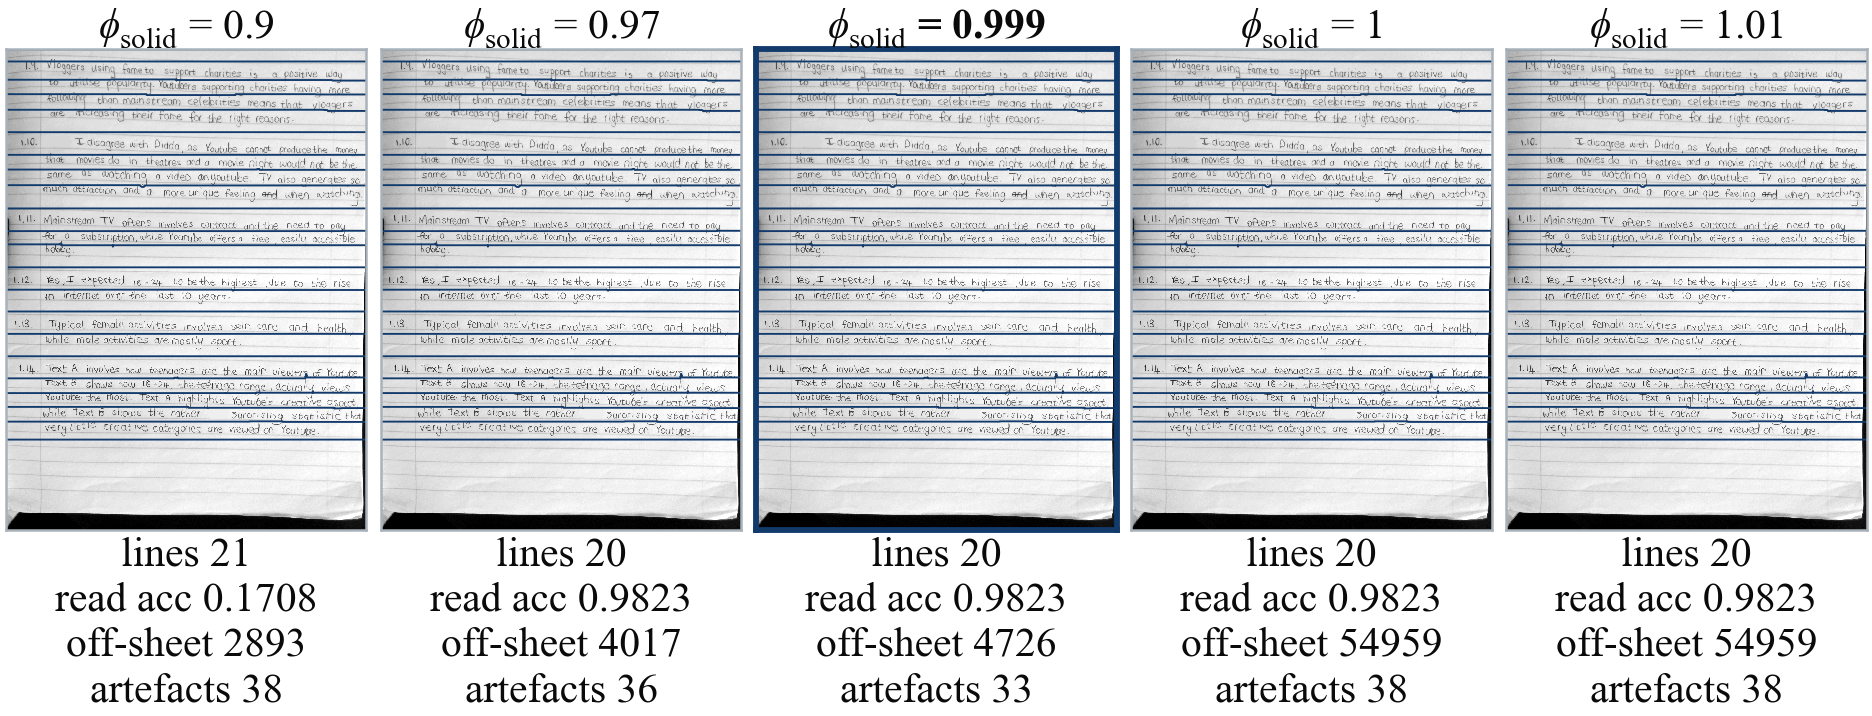
\includegraphics[width=\linewidth]{../figures/solid_block.png}

\caption{Window fill above which a solid block is ruled out as writing. Each panel is the same input processed by the submitted code with only $\phi_{\text{solid}}$ changed; the panel outlined in dark blue is the submitted value.}

\label{fig:solid-block}

\end{figure}

\begin{figure}[htbp]

\centering

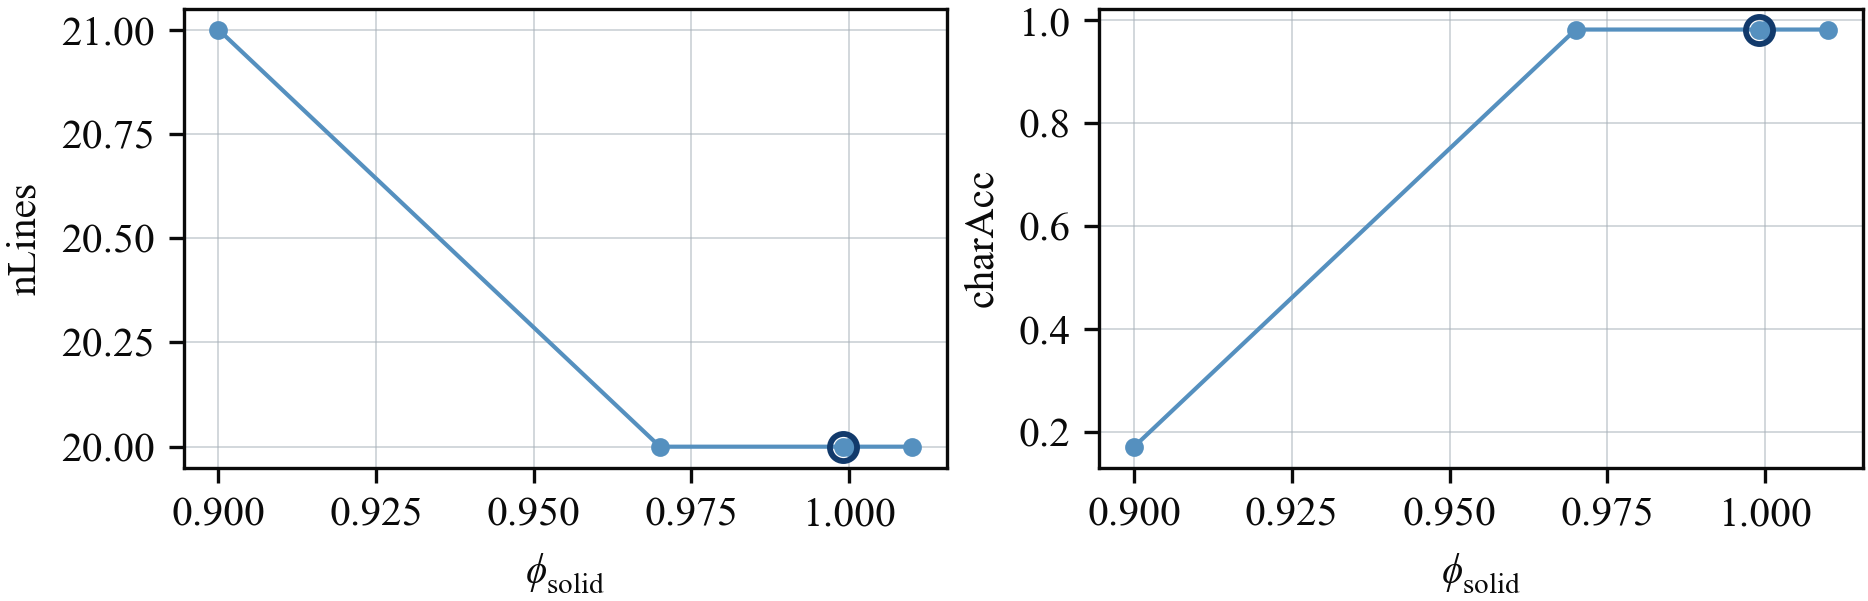
\includegraphics[width=\linewidth]{../figures/solid_block_trend.png}

\caption{Window fill above which a solid block is ruled out as writing: measured quantities against the swept value. The circled point is the submitted value.}

\end{figure}

\begin{table}[htbp]
\centering
\small
\caption{Window fill above which a solid block is ruled out as writing: measured effect of each swept value. The submitted value is in bold.}
\begin{tabular}{lrrrr}
\toprule
\$\textbackslash\{\}phi\_\{\textbackslash\{\}text\{solid\}\}\$ & \textsf{nLines} & \textsf{charAcc} & \textsf{inkOutsidePaper} & \textsf{artifactPieces} \\
\midrule
0.9 & 21 & 0.1708 & 2893 & 38 \\
0.97 & 20 & 0.9823 & 4017 & 36 \\
\bfseries 0.999 & \bfseries 20 & \bfseries 0.9823 & \bfseries 4726 & \bfseries 33 \\
1 & 20 & 0.9823 & 54959 & 38 \\
1.01 & 20 & 0.9823 & 54959 & 38 \\
\bottomrule
\end{tabular}
\end{table}

\section{Sheet detection}

\subsection{Fraction of the median brightness below which a block is off-sheet}

\label{coef:paper-dark}

\begin{description}[leftmargin=5.2em,style=sameline]

\item[Symbol] $\tau_{\text{paper}}$

\item[Value] \texttt{0.45}

\item[Source] \texttt{segment.py}, \texttt{PaperRegionMask}

\item[Swept] \texttt{0.25}, \texttt{0.35}, \texttt{0.45}, \texttt{0.6}, \texttt{0.75}

\end{description}

\paragraph{Basis}

Finding the page as the largest bright connected region of a block-averaged image follows the standard camera-document pre-processing pipeline \cite{shafait2008}; the labelling is \cite{rosenfeld1966}.

\paragraph{Why this value}

The sheet is the brightest large object in the photograph and the desk around it is darker. Comparing against the \emph{median} of the block-averaged image rather than a fixed grey makes the test independent of exposure: the median of a photograph that is mostly paper is the paper level. A desk, a shadow or the edge of the frame is well under half the paper level, while shading on the sheet itself rarely falls below $0.6$ of it, so $0.45$ separates the two with margin on both sides.

\paragraph{What the coefficient does}

The test runs on a $4\times4$ block average, so it is a judgement about regions, not pixels, and the writing itself does not drag a block under the limit. Raising $\tau_{\text{paper}}$ eats into the sheet and can clip a whole margin of writing; lowering it lets the desk in, and the largest bright blob then spans the sheet and its surroundings.

\paragraph{Alternatives considered}

Edge detection and a quadrilateral fit \cite{canny1986} to find the sheet corners, which is more precise but fails when a corner is out of frame; or assuming the whole frame is paper, which the guard \texttt{dark.mean()<0.002} already falls back to when almost nothing is dark.

\paragraph{Worked example}

On the probe page the sheet covers $94.7\%$ of the frame at the submitted setting and $4726$ mask pixels lie outside it and are removed.

\paragraph{What the sweep actually showed}

The detected sheet shrinks steadily as the limit rises --- coverage $0.954$, $0.950$, $0.947$, $0.943$, $0.901$ --- and the last step is the telling one. At $\tau_{\text{paper}} = 0.75$ the sheet has lost $4.6$ percentage points of the frame, the ink falling outside it jumps from $4\,726$ to $12\,615$ pixels, and one line of writing is lost entirely ($19$ lines found against $20$ in the transcript). That is the failure the coefficient has to avoid: shading on the sheet itself being read as off-sheet, taking a margin of real writing with it. The submitted value sits two steps away from that cliff.

\begin{figure}[htbp]

\centering

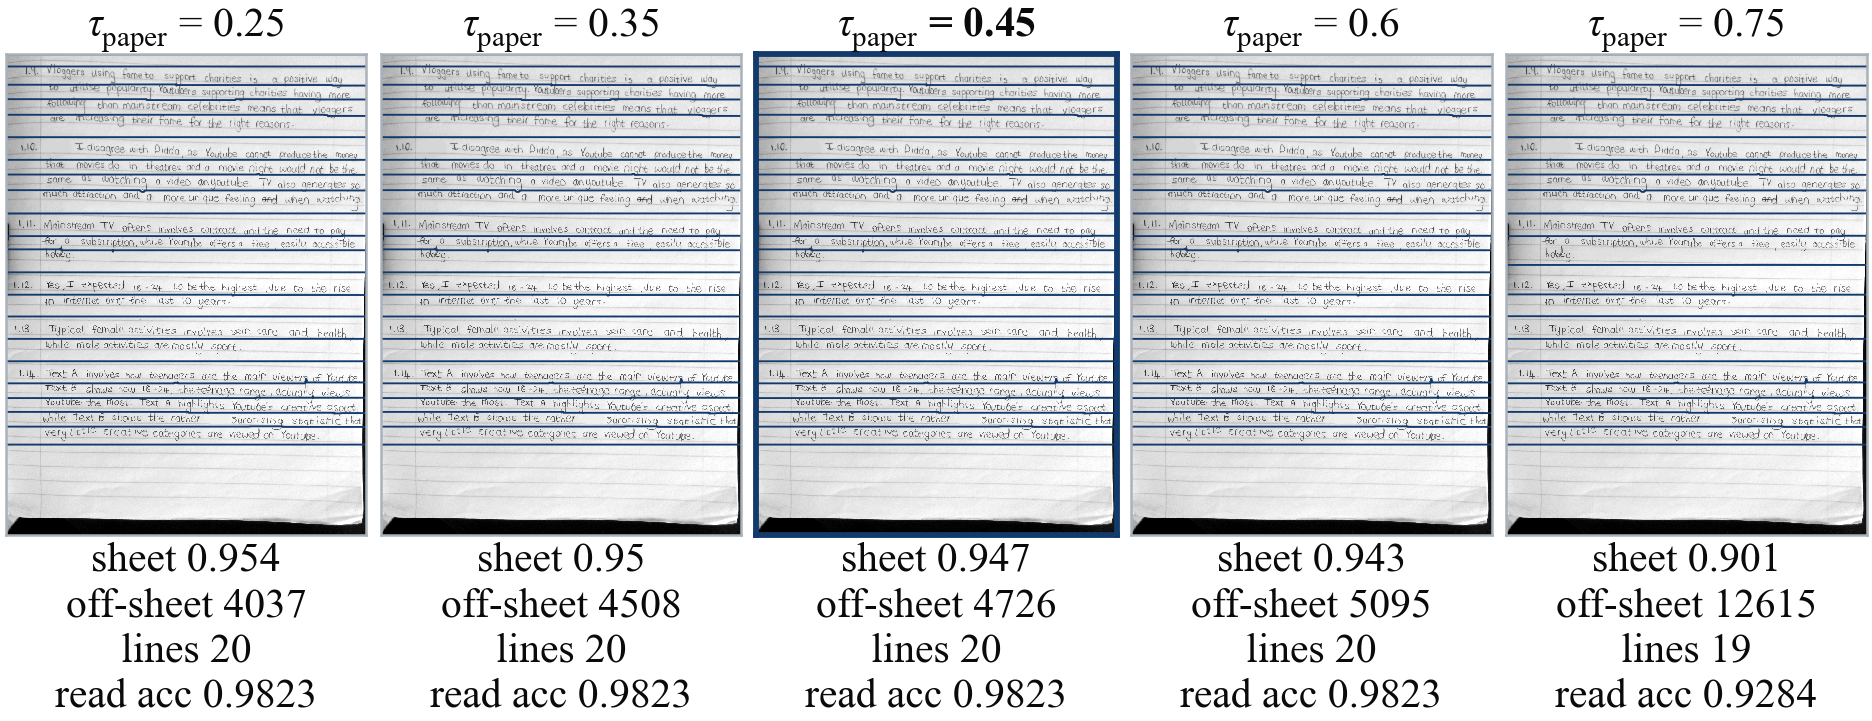
\includegraphics[width=\linewidth]{../figures/paper_dark.png}

\caption{Fraction of the median brightness below which a block is off-sheet. Each panel is the same input processed by the submitted code with only $\tau_{\text{paper}}$ changed; the panel outlined in dark blue is the submitted value.}

\label{fig:paper-dark}

\end{figure}

\begin{figure}[htbp]

\centering

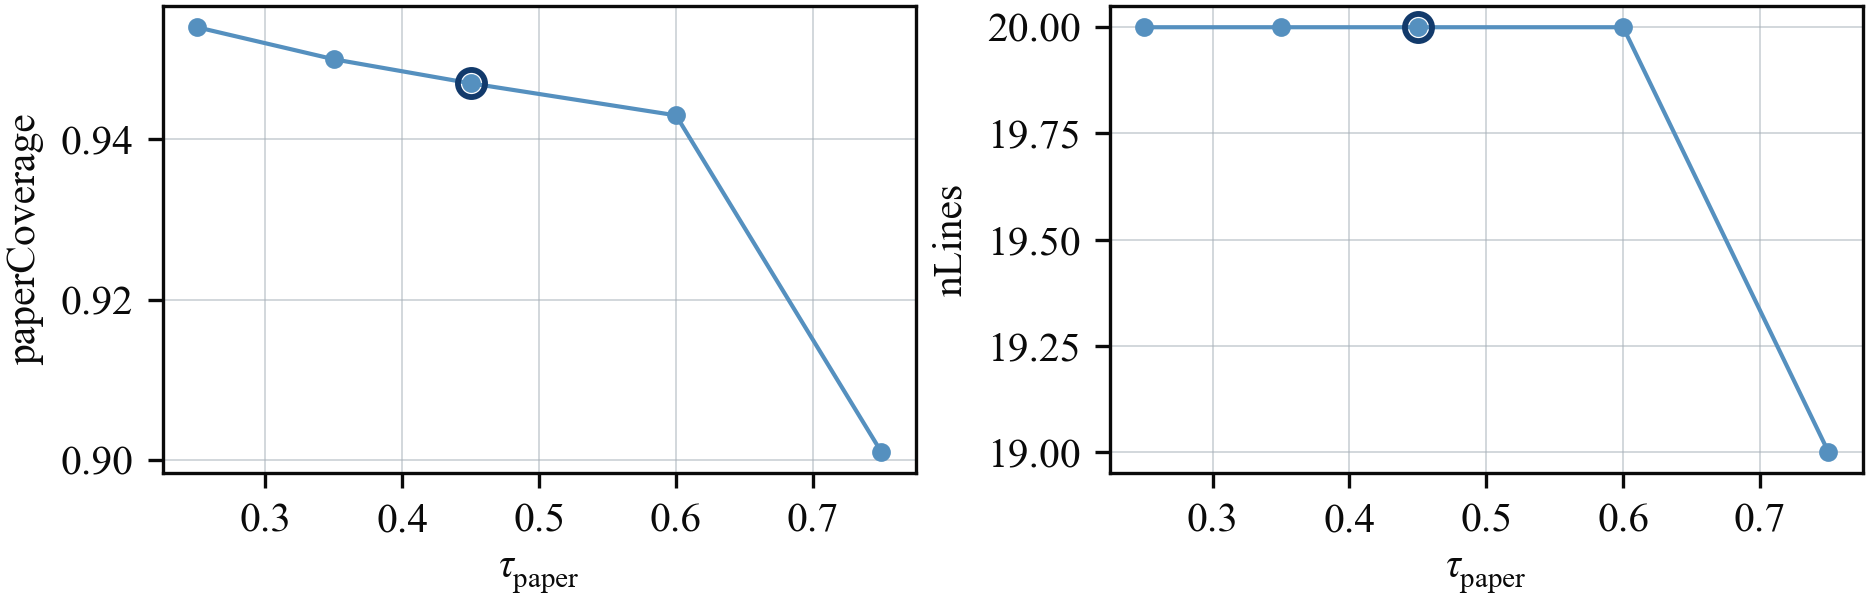
\includegraphics[width=\linewidth]{../figures/paper_dark_trend.png}

\caption{Fraction of the median brightness below which a block is off-sheet: measured quantities against the swept value. The circled point is the submitted value.}

\end{figure}

\begin{table}[htbp]
\centering
\small
\caption{Fraction of the median brightness below which a block is off-sheet: measured effect of each swept value. The submitted value is in bold.}
\begin{tabular}{lrrrr}
\toprule
\$\textbackslash\{\}tau\_\{\textbackslash\{\}text\{paper\}\}\$ & \textsf{paperCoverage} & \textsf{inkOutsidePaper} & \textsf{nLines} & \textsf{charAcc} \\
\midrule
0.25 & 0.954 & 4037 & 20 & 0.9823 \\
0.35 & 0.95 & 4508 & 20 & 0.9823 \\
\bfseries 0.45 & \bfseries 0.947 & \bfseries 4726 & \bfseries 20 & \bfseries 0.9823 \\
0.6 & 0.943 & 5095 & 20 & 0.9823 \\
0.75 & 0.901 & 12615 & 19 & 0.9284 \\
\bottomrule
\end{tabular}
\end{table}

\section{Page orientation}

\subsection{How much better the sideways reading must be before the page is turned}

\label{coef:axis-turn-margin}

\begin{description}[leftmargin=5.2em,style=sameline]

\item[Symbol] $m_{\text{axis}}$

\item[Value] \texttt{1.35}

\item[Source] \texttt{segment.py}, \texttt{UprightPage}

\item[Swept] \texttt{1.0}, \texttt{1.15}, \texttt{1.35}, \texttt{1.6}, \texttt{2.0}

\end{description}

\paragraph{Basis}

Lines of text produce a strongly periodic projection profile along one axis only, which is the signal every profile-based layout method uses \cite{likforman2007,shafait2008}.

\paragraph{Why this value}

The score is the fraction of rows that are nearly empty, which is high across the gaps between lines and low along them. Both orientations are scored and the page is turned only if the sideways score is clearly better. A plain \enquote{greater than} would turn a page whenever noise put the two scores a hair apart, and turning a page wrongly costs the whole job, while failing to turn one the user photographed correctly costs nothing. The margin is therefore asymmetric on purpose, and $1.35$ is far outside the measured spread between the two scores on a correctly held page.

\paragraph{What the coefficient does}

$m_{\text{axis}}$ is a ratio, so it is unaffected by how much ink is on the page. At $1.0$ the test becomes a bare comparison; above the true ratio of a genuinely sideways page it can never fire and a rotated page is never corrected.

\paragraph{Worked example}

On the probe page the two scores are $s_0 = 0.470$ and $s_{90} = 0.075$, a ratio of $0.16$ in favour of leaving it alone, so the page is not turned at any setting in the sweep. The decision has $8.4\times$ margin against the $1.35$ limit.

\paragraph{What the sweep actually showed}

\textbf{No effect was measured}, as predicted. The two axis scores on this page are $s_0 = 0.470$ and $s_{90} = 0.075$, a ratio of $0.16$ in favour of leaving the page alone, so the page is not turned even at $m_{\text{axis}} = 1.0$ where the test is a bare comparison. The decision has $8.4\times$ margin against the submitted limit. This sweep demonstrates the stability of the decision, not the turning; showing the turn would need a page photographed sideways.

\paragraph{Limits of this test}

The probe page is upright, so this sweep demonstrates the stability of the decision rather than the turning itself; the recorded scores show how far the page is from the limit.

\begin{figure}[htbp]

\centering

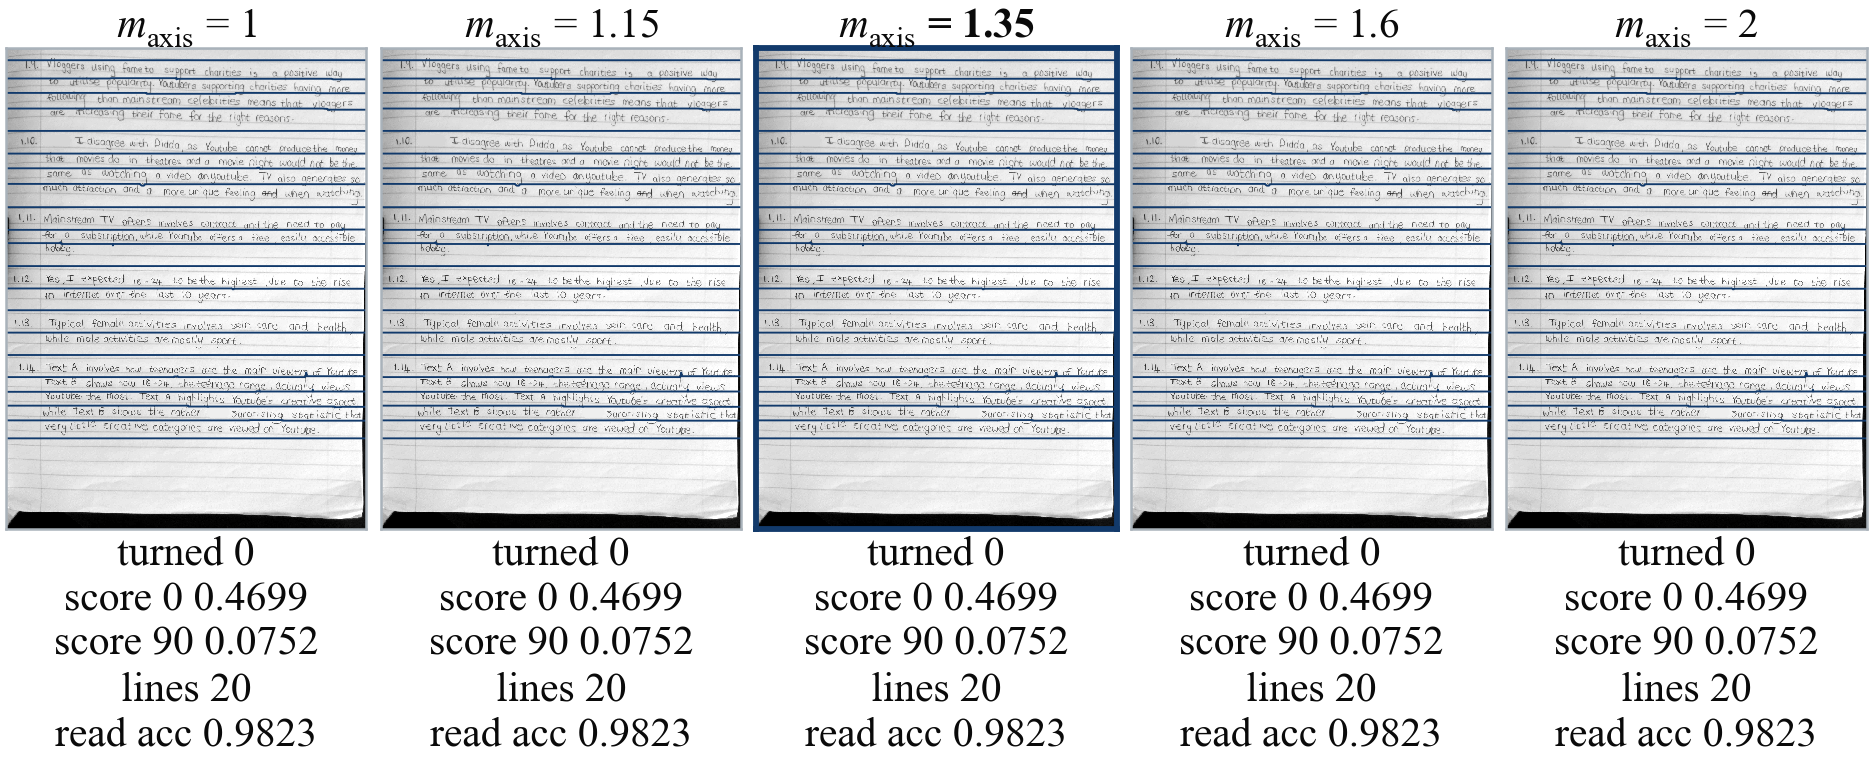
\includegraphics[width=\linewidth]{../figures/axis_turn_margin.png}

\caption{How much better the sideways reading must be before the page is turned. Each panel is the same input processed by the submitted code with only $m_{\text{axis}}$ changed; the panel outlined in dark blue is the submitted value.}

\label{fig:axis-turn-margin}

\end{figure}

\begin{figure}[htbp]

\centering

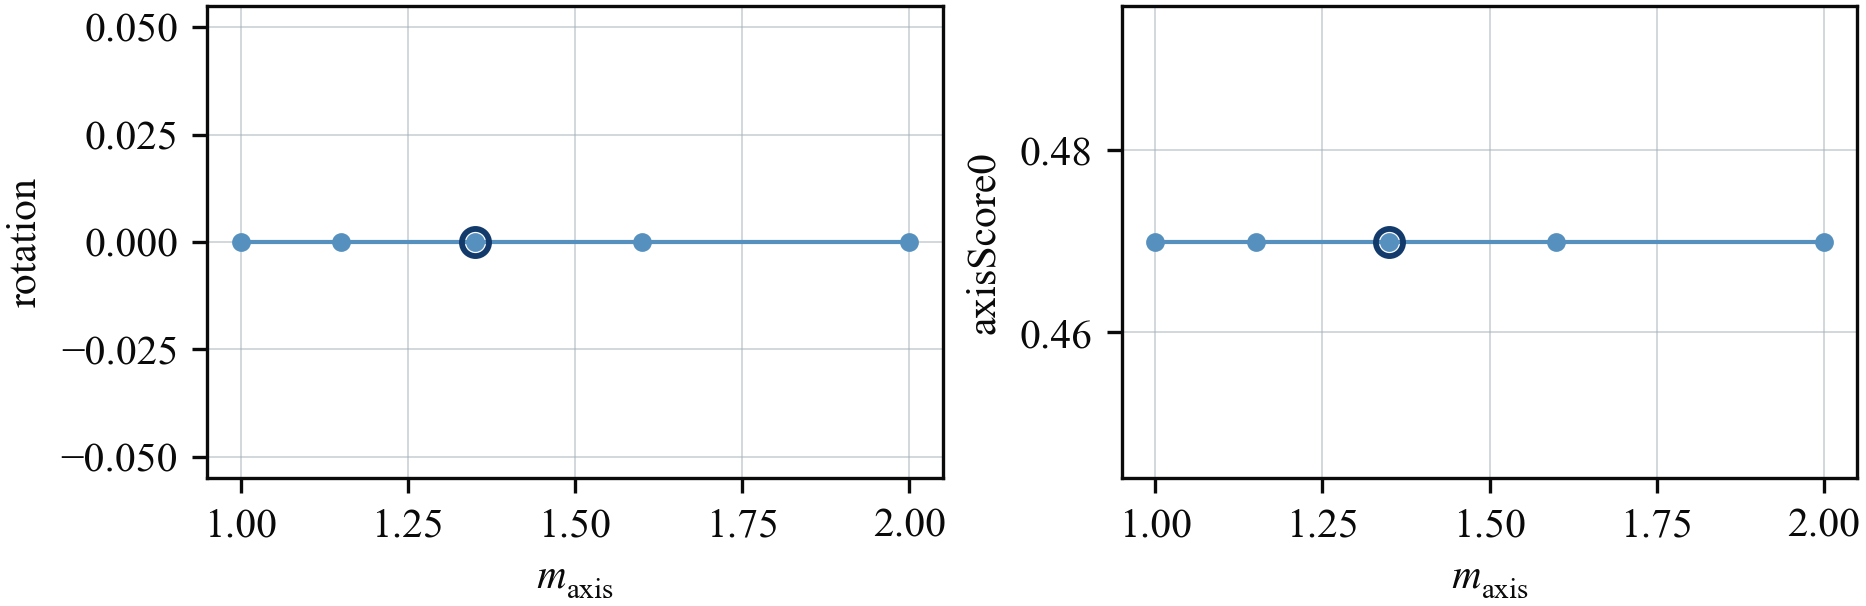
\includegraphics[width=\linewidth]{../figures/axis_turn_margin_trend.png}

\caption{How much better the sideways reading must be before the page is turned: measured quantities against the swept value. The circled point is the submitted value.}

\end{figure}

\begin{table}[htbp]
\centering
\small
\caption{How much better the sideways reading must be before the page is turned: measured effect of each swept value. The submitted value is in bold.}
\begin{tabular}{lrrrrr}
\toprule
\$m\_\{\textbackslash\{\}text\{axis\}\}\$ & \textsf{rotation} & \textsf{axisScore0} & \textsf{axisScore90} & \textsf{nLines} & \textsf{charAcc} \\
\midrule
1 & 0 & 0.4699 & 0.0752 & 20 & 0.9823 \\
1.15 & 0 & 0.4699 & 0.0752 & 20 & 0.9823 \\
\bfseries 1.35 & \bfseries 0 & \bfseries 0.4699 & \bfseries 0.0752 & \bfseries 20 & \bfseries 0.9823 \\
1.6 & 0 & 0.4699 & 0.0752 & 20 & 0.9823 \\
2 & 0 & 0.4699 & 0.0752 & 20 & 0.9823 \\
\bottomrule
\end{tabular}
\end{table}

\section{Line finding}

\subsection{Profile height a candidate line peak must reach}

\label{coef:peak-floor}

\begin{description}[leftmargin=5.2em,style=sameline]

\item[Symbol] $\tau_{\text{peak}}$

\item[Value] \texttt{0.06}

\item[Source] \texttt{segment.py}, \texttt{LineCentres}

\item[Swept] \texttt{0.02}, \texttt{0.04}, \texttt{0.06}, \texttt{0.12}, \texttt{0.2}

\end{description}

\paragraph{Basis}

Peak picking on a smoothed horizontal projection profile is the classical line-finding method \cite{likforman2007}; the profile and its use on handwritten pages follow \cite{marti2002}.

\paragraph{Why this value}

Every local maximum of the smoothed ink-per-row profile is a candidate line centre, but a short line, a stray mark or the tail of a descender also makes a bump. The floor is relative to the tallest peak on the page, so it does not depend on how much was written. It has to sit below the weakest real line, which on these pages is a one- or two-word last line carrying roughly a tenth of the ink of a full line, and above the texture left after smoothing. $0.06$ is below that weakest-line level with margin.

\paragraph{What the coefficient does}

This floor controls how many candidates reach the separation test that follows; it cannot by itself create a line, because the $0.6P$ separation rule then thins the candidates out. Raising it drops genuine short lines outright, which is unrecoverable: there is no later stage that puts a line back.

\paragraph{Alternatives considered}

Prominence-based peak picking, which \texttt{train.py} does implement in \texttt{FindPeaks} with an explicit prominence and distance, or fitting a fixed pitch and taking every period, which fails on a page whose last line is short.

\paragraph{Worked example}

The probe page has $20$ transcript lines. The sweep records how many the segmenter returns at each floor, against that known count.

\paragraph{What the sweep actually showed}

This is the clearest result in the segmentation group. Below the submitted value the page over-segments --- $21$ lines at both $0.02$ and $0.04$ against $20$ in the transcript --- and above it the page under-segments, $19$ lines at both $0.12$ and $0.20$. The submitted $0.06$ is the only one of the five that recovers exactly the right number of lines. The reading score shows the over-segmentation case costing far more than the under-segmentation one, $0.173$ against $0.982$, because an extra line early on shifts every later crop against the transcript.

\begin{figure}[htbp]

\centering

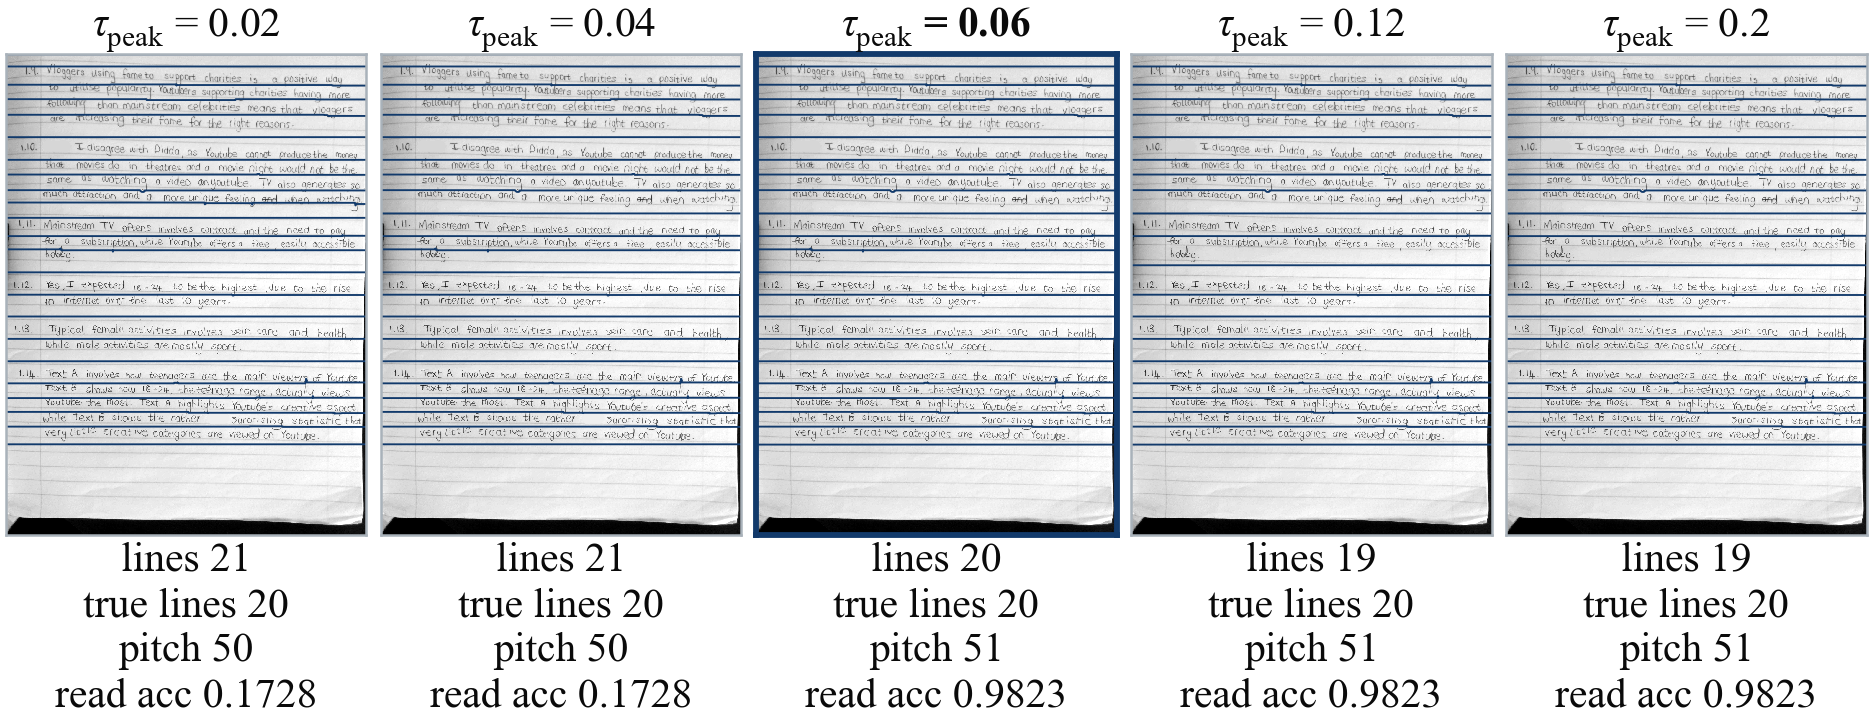
\includegraphics[width=\linewidth]{../figures/peak_floor.png}

\caption{Profile height a candidate line peak must reach. Each panel is the same input processed by the submitted code with only $\tau_{\text{peak}}$ changed; the panel outlined in dark blue is the submitted value.}

\label{fig:peak-floor}

\end{figure}

\begin{figure}[htbp]

\centering

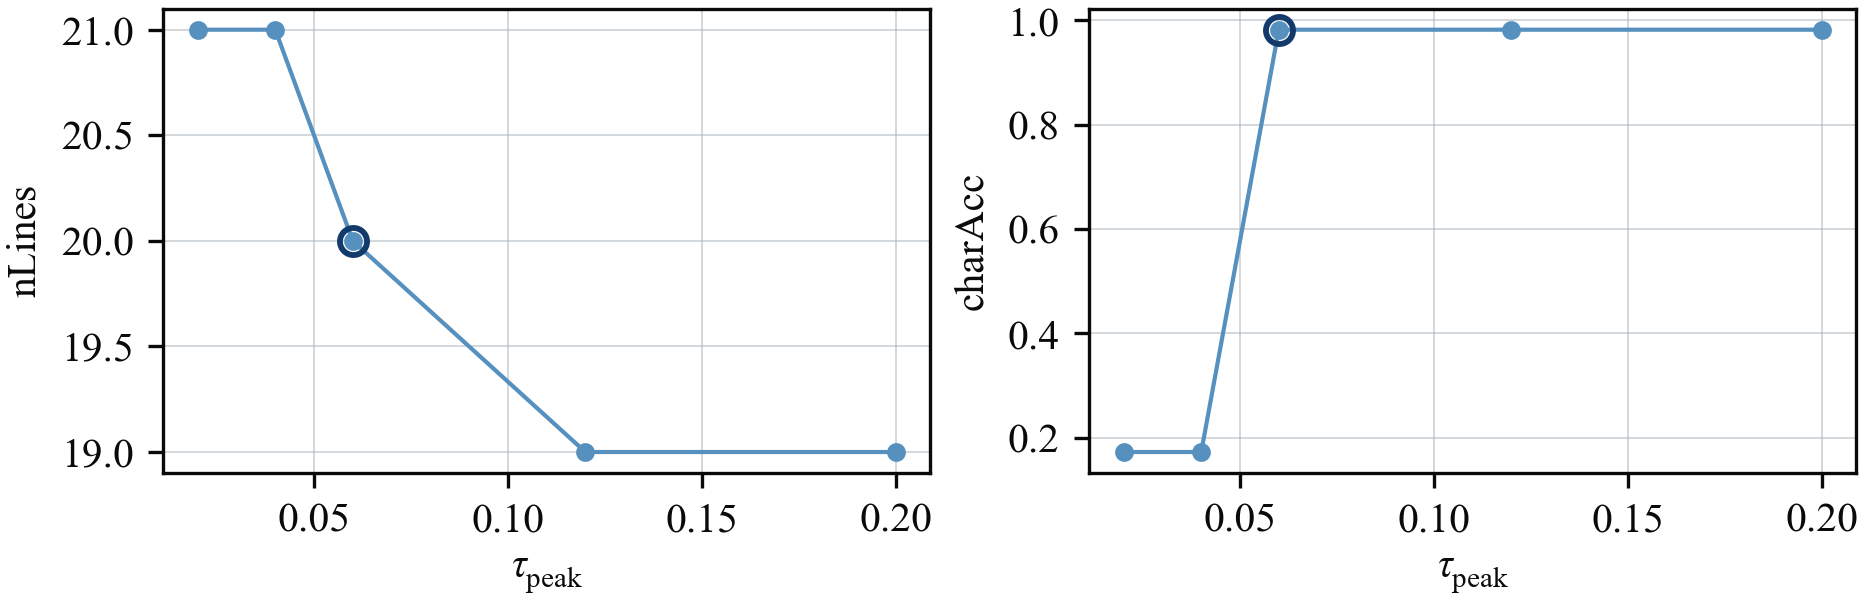
\includegraphics[width=\linewidth]{../figures/peak_floor_trend.png}

\caption{Profile height a candidate line peak must reach: measured quantities against the swept value. The circled point is the submitted value.}

\end{figure}

\begin{table}[htbp]
\centering
\small
\caption{Profile height a candidate line peak must reach: measured effect of each swept value. The submitted value is in bold.}
\begin{tabular}{lrrrr}
\toprule
\$\textbackslash\{\}tau\_\{\textbackslash\{\}text\{peak\}\}\$ & \textsf{nLines} & \textsf{nLinesTruth} & \textsf{pitch} & \textsf{charAcc} \\
\midrule
0.02 & 21 & 20 & 50 & 0.1728 \\
0.04 & 21 & 20 & 50 & 0.1728 \\
\bfseries 0.06 & \bfseries 20 & \bfseries 20 & \bfseries 51 & \bfseries 0.9823 \\
0.12 & 19 & 20 & 51 & 0.9823 \\
0.2 & 19 & 20 & 51 & 0.9823 \\
\bottomrule
\end{tabular}
\end{table}

\subsection{Smallest spacing between two accepted line centres}

\label{coef:centre-separation}

\begin{description}[leftmargin=5.2em,style=sameline]

\item[Symbol] $s_{\min}$

\item[Value] \texttt{0.6}

\item[Source] \texttt{segment.py}, \texttt{LineCentres}

\item[Swept] \texttt{0.3}, \texttt{0.45}, \texttt{0.6}, \texttt{0.8}, \texttt{1.0}

\end{description}

\paragraph{Basis}

Enforcing a minimum distance between accepted peaks is the usual non-maximum suppression step of profile line finding \cite{likforman2007}.

\paragraph{Why this value}

Candidates are taken strongest first and a new one is accepted only if it is at least $s_{\min}$ pitches from every centre already kept. The limit is expressed in measured line pitch $P$, not pixels, so it follows the page. Two real lines are one pitch apart by definition, so anything below $1.0$ admits them both; the profile of a single line, however, is double-humped when the writing has many ascenders, and those humps sit a few tenths of a pitch apart. $0.6$ is above that internal structure and safely below the one-pitch spacing of real lines.

\paragraph{What the coefficient does}

Taken with the peak floor this is the whole line-count decision. Too small and one line is reported as two, which splits words across crops; too large and two closely written lines are merged into one crop, which the reader then cannot transcribe. Because candidates are sorted by strength, the rule keeps the strongest of a cluster rather than the first.

\paragraph{Alternatives considered}

Merging on the depth of the valley between two peaks, which this code also implements as \texttt{LINE\_MERGE\_VALLEY} and leaves disabled, or a fixed pitch comb.

\paragraph{Worked example}

On the probe page $P = 51$ px at half resolution, so $0.6P = 30.6$ px: two centres closer than $31$ px are treated as one line.

\paragraph{What the sweep actually showed}

The decisive value is the largest. At $s_{\min} = 1.0$ the segmenter returns \textbf{14} lines where the transcript has $20$: requiring a full pitch between centres merges closely written lines, six of them on this page. The reading score falls to $0.647$ accordingly, which as section~\ref{sec:readacc} explains is mostly the crop-to-transcript pairing breaking rather than the crops becoming unreadable. Between $0.3$ and $0.8$ the line count is correct at $20$ and nothing else moves, so on this page the submitted value sits in the middle of a wide safe plateau rather than on a knife edge.

\begin{figure}[htbp]

\centering

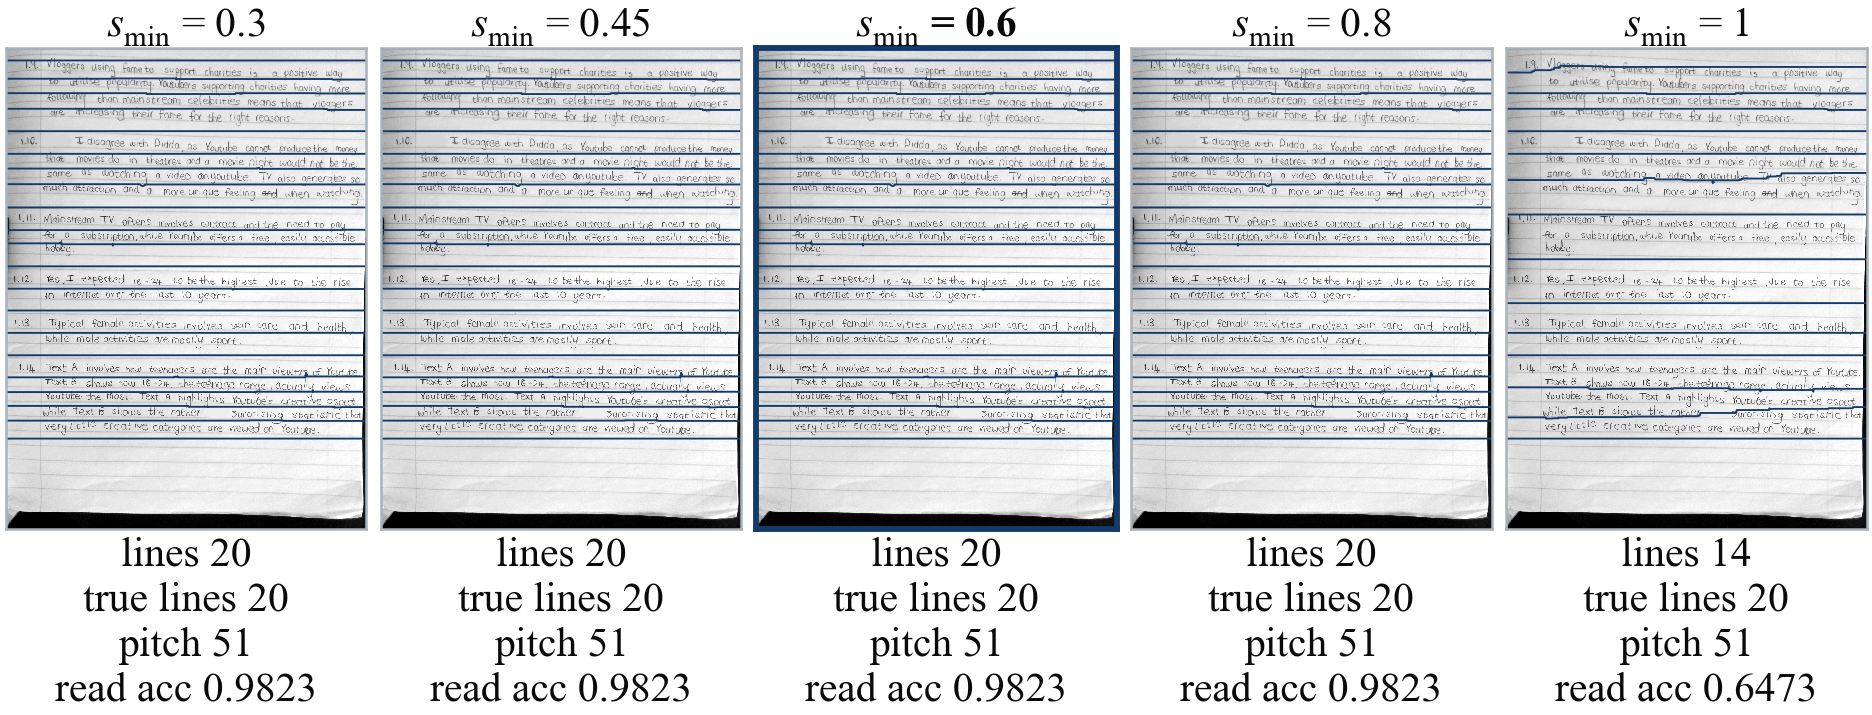
\includegraphics[width=\linewidth]{../figures/centre_separation.png}

\caption{Smallest spacing between two accepted line centres. Each panel is the same input processed by the submitted code with only $s_{\min}$ changed; the panel outlined in dark blue is the submitted value.}

\label{fig:centre-separation}

\end{figure}

\begin{figure}[htbp]

\centering

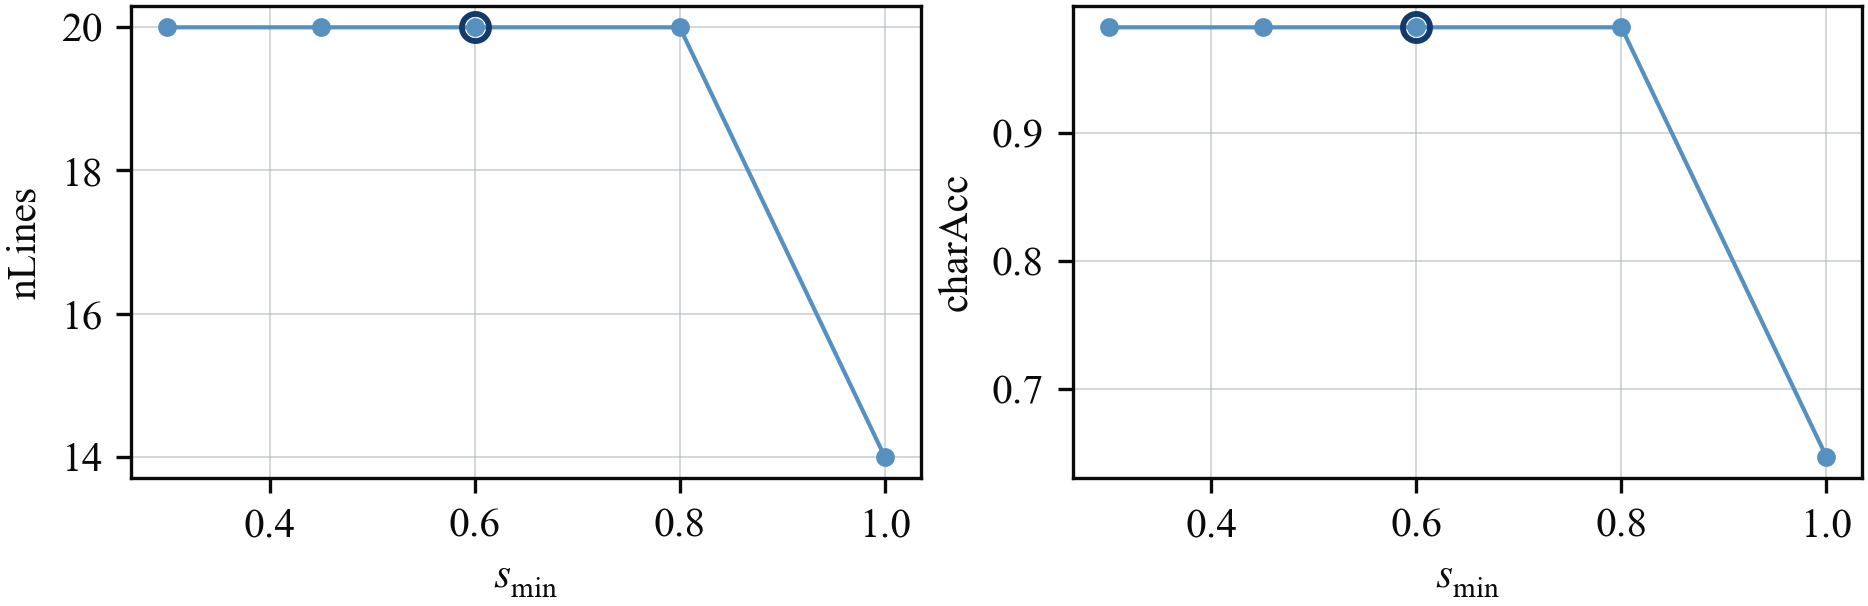
\includegraphics[width=\linewidth]{../figures/centre_separation_trend.png}

\caption{Smallest spacing between two accepted line centres: measured quantities against the swept value. The circled point is the submitted value.}

\end{figure}

\begin{table}[htbp]
\centering
\small
\caption{Smallest spacing between two accepted line centres: measured effect of each swept value. The submitted value is in bold.}
\begin{tabular}{lrrrr}
\toprule
\$s\_\{\textbackslash\{\}min\}\$ & \textsf{nLines} & \textsf{nLinesTruth} & \textsf{pitch} & \textsf{charAcc} \\
\midrule
0.3 & 20 & 20 & 51 & 0.9823 \\
0.45 & 20 & 20 & 51 & 0.9823 \\
\bfseries 0.6 & \bfseries 20 & \bfseries 20 & \bfseries 51 & \bfseries 0.9823 \\
0.8 & 20 & 20 & 51 & 0.9823 \\
1 & 14 & 20 & 51 & 0.6473 \\
\bottomrule
\end{tabular}
\end{table}

\subsection{Valley depth below which two line centres are merged}

\label{coef:line-merge-valley}

\begin{description}[leftmargin=5.2em,style=sameline]

\item[Symbol] $\tau_{\text{valley}}$

\item[Value] \texttt{1.0}

\item[Source] \texttt{segment.py}, \texttt{LineCentres}

\item[Swept] \texttt{0.3}, \texttt{0.5}, \texttt{0.7}, \texttt{0.9}, \texttt{1.0}

\end{description}

\paragraph{Basis}

Merging profile peaks separated only by a shallow valley is the standard refinement where projection peaks over-segment \cite{likforman2007}.

\paragraph{Why this value}

This is a second, optional merge: for each adjacent pair of centres the lowest profile value between them is compared with the smaller of the two peaks, and the pair is merged if the dip is shallow. The submitted value is $1.0$, and the loop is guarded by \texttt{thr<1.0}, so \textbf{the merge is switched off in the submitted system}. That is the honest description of this coefficient: it is a disabled mechanism, kept because \texttt{SegmentLines} exposes \texttt{mergeValley} as an argument so a difficult page can be re-run with it on.

\paragraph{What the coefficient does}

The value is a ratio of ink depths, so $1.0$ means \enquote{merge even when the valley is as high as the peak}, which is why it is used as the off switch rather than a large number. Lowering it to $0.7$ merges only genuinely shallow dips.

\paragraph{Alternatives considered}

Leaving over-segmentation to the ownership stage, which is what happens now, or topological persistence on the profile, which is the same idea with a cleaner definition.

\paragraph{Worked example}

With $\tau_{\text{valley}} = 1.0$ the \texttt{while} test $1.0 < 1.0$ is false and no merge is ever attempted, so the sweep shows what the project chose not to use.

\paragraph{What the sweep actually showed}

\textbf{Nothing changed at any value}, which is the expected result and is the point of including it. The merge loop is guarded by \texttt{thr<1.0} and the submitted value is $1.0$, so the merge never runs in the submitted system. The four lower values do enable it, and still nothing changed, which says that on this page no adjacent pair of line centres has a valley shallow enough to merge even at $\tau_{\text{valley}} = 0.3$. The mechanism is intact and unused.

\begin{figure}[htbp]

\centering

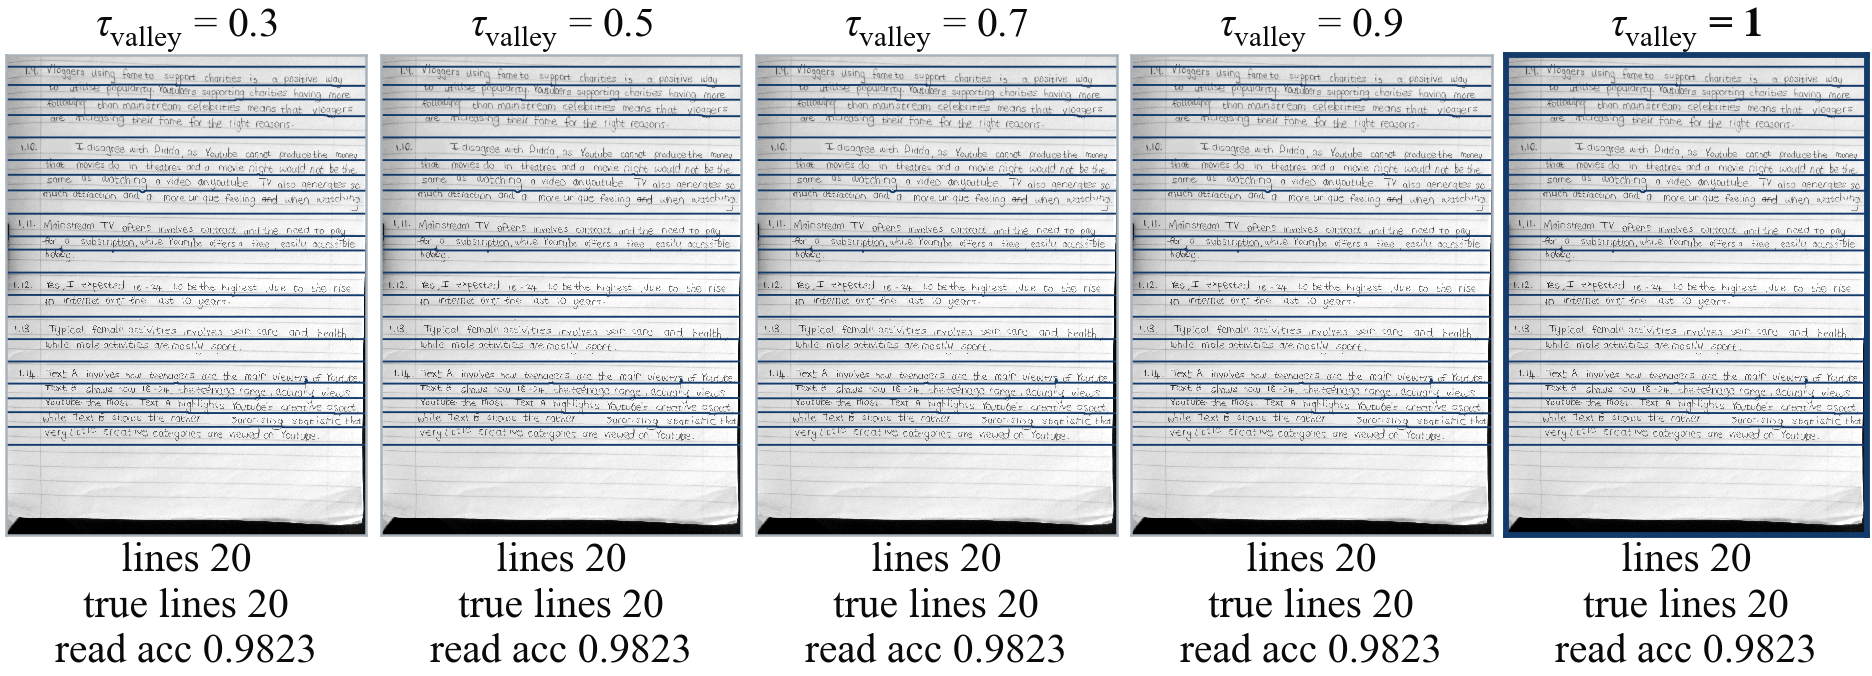
\includegraphics[width=\linewidth]{../figures/line_merge_valley.png}

\caption{Valley depth below which two line centres are merged. Each panel is the same input processed by the submitted code with only $\tau_{\text{valley}}$ changed; the panel outlined in dark blue is the submitted value.}

\label{fig:line-merge-valley}

\end{figure}

\begin{figure}[htbp]

\centering

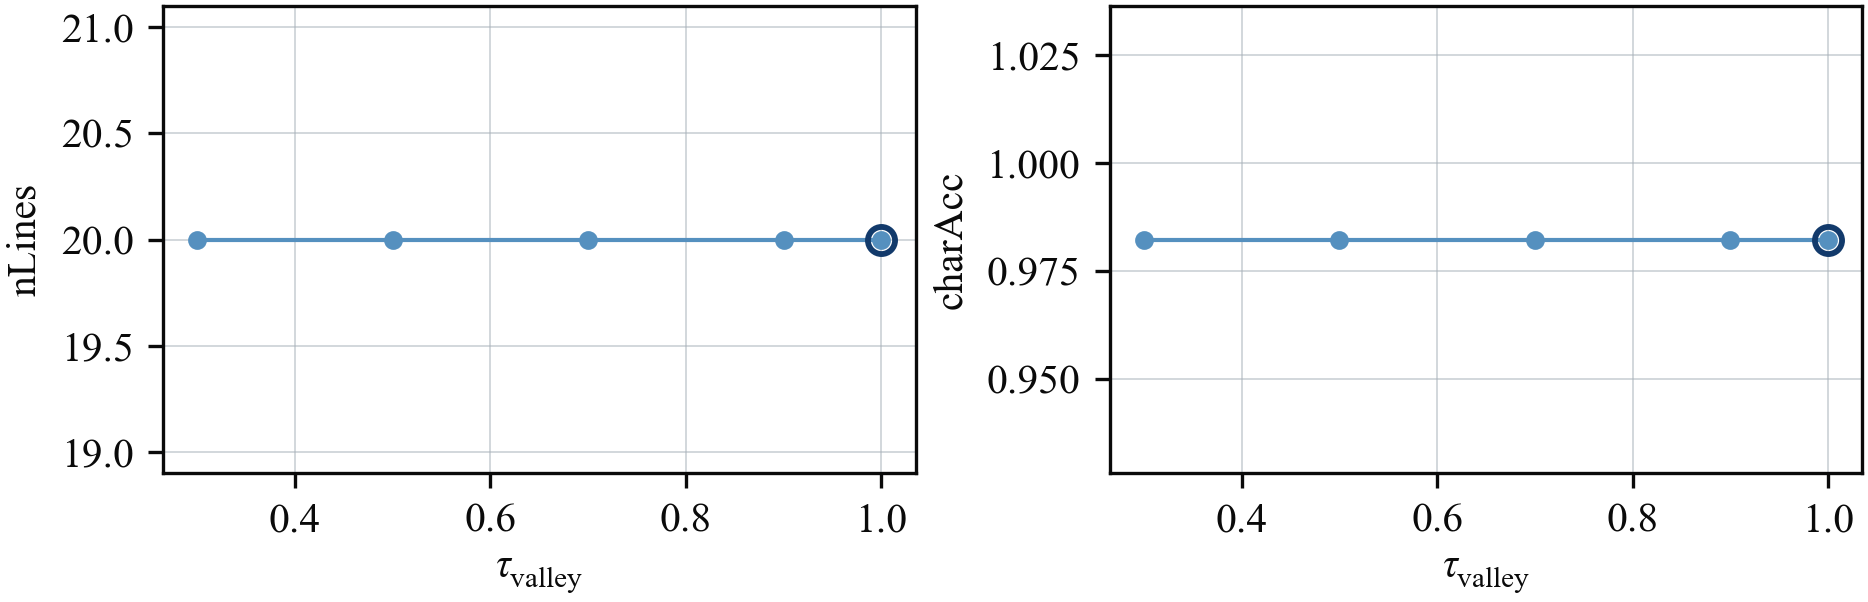
\includegraphics[width=\linewidth]{../figures/line_merge_valley_trend.png}

\caption{Valley depth below which two line centres are merged: measured quantities against the swept value. The circled point is the submitted value.}

\end{figure}

\begin{table}[htbp]
\centering
\small
\caption{Valley depth below which two line centres are merged: measured effect of each swept value. The submitted value is in bold.}
\begin{tabular}{lrrr}
\toprule
\$\textbackslash\{\}tau\_\{\textbackslash\{\}text\{valley\}\}\$ & \textsf{nLines} & \textsf{nLinesTruth} & \textsf{charAcc} \\
\midrule
0.3 & 20 & 20 & 0.9823 \\
0.5 & 20 & 20 & 0.9823 \\
0.7 & 20 & 20 & 0.9823 \\
0.9 & 20 & 20 & 0.9823 \\
\bfseries 1 & \bfseries 20 & \bfseries 20 & \bfseries 0.9823 \\
\bottomrule
\end{tabular}
\end{table}

\subsection{Smallest peak gap counted as line spacing, in letter heights}

\label{coef:pitch-peak-floor-xh}

\begin{description}[leftmargin=5.2em,style=sameline]

\item[Symbol] $g_{\min}$

\item[Value] \texttt{1.5}

\item[Source] \texttt{segment.py}, \texttt{LinePitch}

\item[Swept] \texttt{0.8}, \texttt{1.2}, \texttt{1.5}, \texttt{2.0}, \texttt{2.5}

\end{description}

\paragraph{Basis}

Line pitch from the median gap between profile peaks, with autocorrelation as a fallback, follows standard profile analysis \cite{likforman2007}.

\paragraph{Why this value}

The median peak gap is only the line pitch if the peaks are different lines. Within one line the profile has structure at the scale of a letter, so a gap of about one letter height is internal and a gap of about two is between lines. The floor is written in median letter heights, measured independently by \texttt{\_LetterHeight}, and $1.5$ sits between those two cases. If the median gap falls below it the estimate is rejected and the autocorrelation fallback is used instead, so the coefficient selects between two estimators rather than setting the pitch itself.

\paragraph{What the coefficient does}

Too low and intra-line structure is accepted as the pitch, which makes $P$ far too small and every $P$-scaled test in the segmenter too tight. Too high and the peak estimator is always rejected in favour of autocorrelation, which is more robust but blind to a page with only two or three lines.

\paragraph{Worked example}

On the probe page the median letter height is such that the peak estimate is accepted and $P = 51$ px at half resolution, against a ruling of $8.4$ mm on the real page.

\paragraph{What the sweep actually showed}

\textbf{No effect was measured}: the estimated pitch stays at $51$ px and the line count at $20$ for every value from $0.8$ to $2.5$. The reason is that on this page the median gap between profile peaks is comfortably above even $2.5$ letter heights, so the peak estimator is accepted at every setting and the autocorrelation fallback is never reached. The coefficient selects between two estimators, and on this input the choice is never close. A page with cramped or irregular line spacing would be needed to exercise it.

\begin{figure}[htbp]

\centering

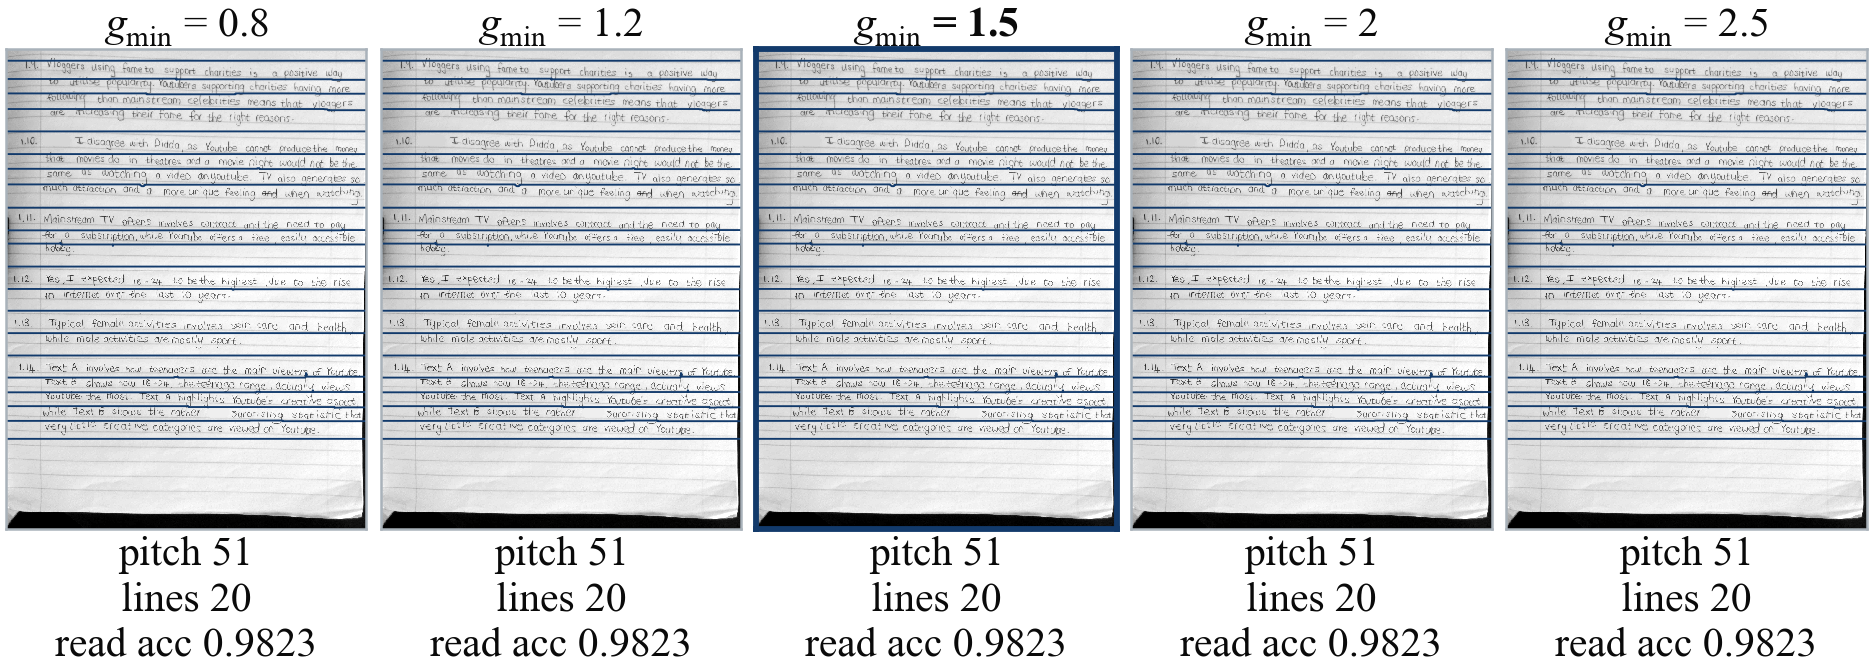
\includegraphics[width=\linewidth]{../figures/pitch_peak_floor_xh.png}

\caption{Smallest peak gap counted as line spacing, in letter heights. Each panel is the same input processed by the submitted code with only $g_{\min}$ changed; the panel outlined in dark blue is the submitted value.}

\label{fig:pitch-peak-floor-xh}

\end{figure}

\begin{figure}[htbp]

\centering

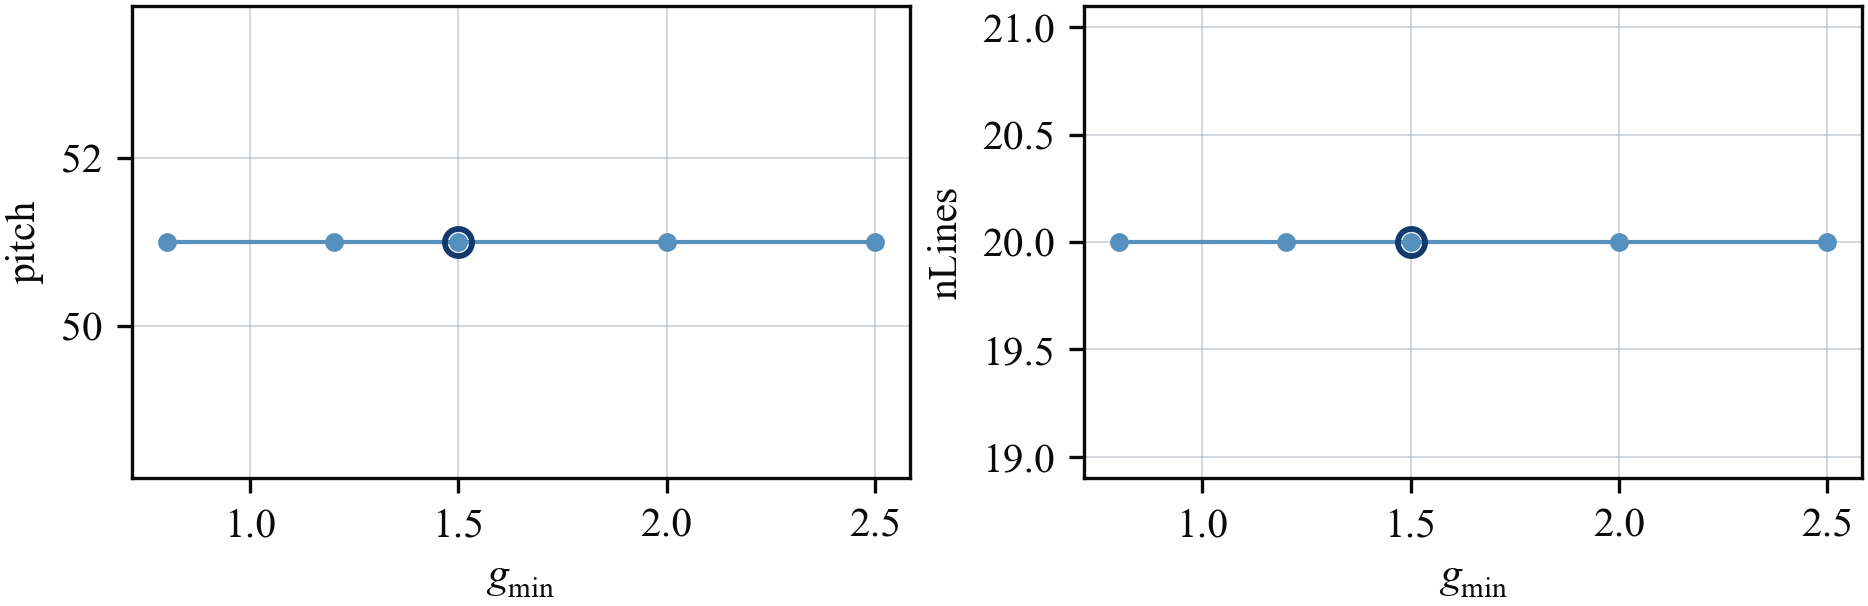
\includegraphics[width=\linewidth]{../figures/pitch_peak_floor_xh_trend.png}

\caption{Smallest peak gap counted as line spacing, in letter heights: measured quantities against the swept value. The circled point is the submitted value.}

\end{figure}

\begin{table}[htbp]
\centering
\small
\caption{Smallest peak gap counted as line spacing, in letter heights: measured effect of each swept value. The submitted value is in bold.}
\begin{tabular}{lrrr}
\toprule
\$g\_\{\textbackslash\{\}min\}\$ & \textsf{pitch} & \textsf{nLines} & \textsf{charAcc} \\
\midrule
0.8 & 51 & 20 & 0.9823 \\
1.2 & 51 & 20 & 0.9823 \\
\bfseries 1.5 & \bfseries 51 & \bfseries 20 & \bfseries 0.9823 \\
2 & 51 & 20 & 0.9823 \\
2.5 & 51 & 20 & 0.9823 \\
\bottomrule
\end{tabular}
\end{table}

\section{Printed-structure removal}

\subsection{Length above which a flat run on the page is printed structure}

\label{coef:rule-flat-len}

\begin{description}[leftmargin=5.2em,style=sameline]

\item[Symbol] $L_{\text{flat}}$

\item[Value] \texttt{1.25}

\item[Source] \texttt{segment.py}, \texttt{RemovePrintedStructure}

\item[Swept] \texttt{0.6}, \texttt{0.9}, \texttt{1.25}, \texttt{1.8}, \texttt{2.5}

\end{description}

\paragraph{Basis}

Long-run detection for printed rules and table borders is the classical morphological approach \cite{haralick1987}, and removing ruling before layout analysis is standard for camera-captured forms \cite{shafait2008}.

\paragraph{Why this value}

On a whole page the printed ruling is horizontal and runs much further than any pen stroke. The limit is written in line pitches $P$, which is measured on the page itself, so it adapts to how large the writing is. One pitch is the distance between successive lines; $1.25P$ is just over that, which no single horizontal pen stroke spans, while a printed rule crosses the whole writing area and so spans many pitches. The run is measured after a one-pixel vertical dilation, so a rule broken by a pen stroke crossing it is still seen as one run.

\paragraph{What the coefficient does}

Lowering $L_{\text{flat}}$ begins to delete the long horizontal parts of the writing itself, which on a cursive page means the baseline carrier stroke joining several letters. Raising it leaves ruling in the mask, where it joins separate lines together and defeats the seam cutter.

\paragraph{Alternatives considered}

A Hough line transform \cite{duda1972} to find the rules explicitly, or removing them from the greyscale by estimating and subtracting the periodic ruling, which also needs the pitch.

\paragraph{Worked example}

On the probe page $P = 51$ px at half resolution, so $1.25P = 63$ px: a flat run must be at least $63$ px long before it is deleted. The submitted setting removes $1988$ pixels of straight structure from this page.

\paragraph{What the sweep actually showed}

The interesting value is $0.85$, where the page returns \textbf{21} lines instead of $20$ and the reading score falls to $0.173$. Shortening the limit to below one line pitch starts deleting long horizontal parts of the writing itself, which breaks a line of writing into pieces and lets a spurious profile peak through. At $0.6$ the removal is larger still ($3\,028$ pixels against $1\,988$) and more artefact pieces are found, $41$ against $33$, but the line count happens to recover --- which is a warning that the line count alone is a coarse health check. Above the submitted value nothing moves, so on this page the risk is entirely on the low side.

\begin{figure}[htbp]

\centering

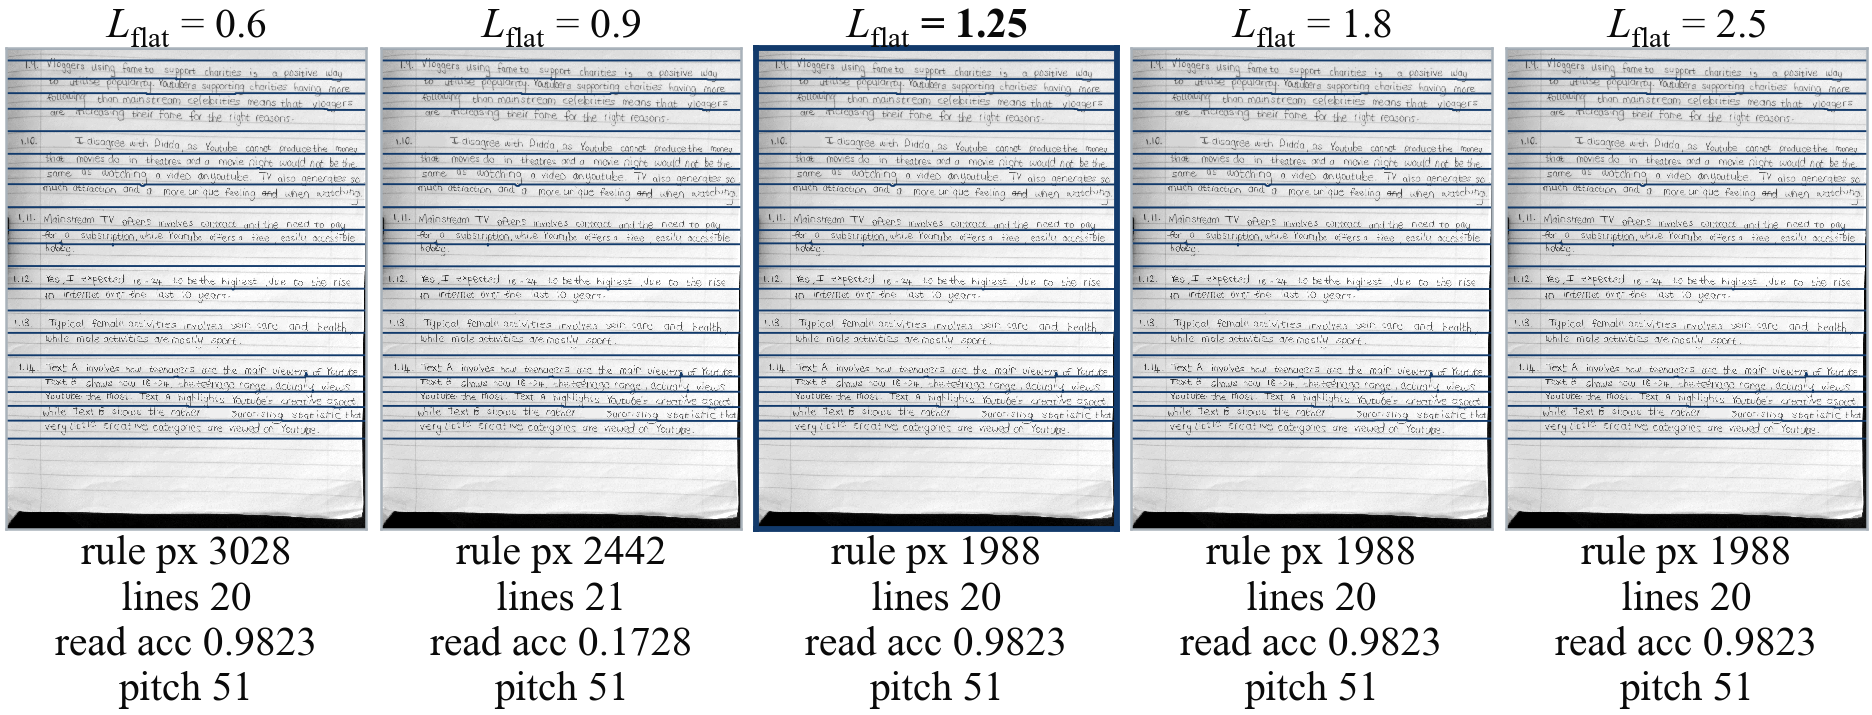
\includegraphics[width=\linewidth]{../figures/rule_flat_len.png}

\caption{Length above which a flat run on the page is printed structure. Each panel is the same input processed by the submitted code with only $L_{\text{flat}}$ changed; the panel outlined in dark blue is the submitted value.}

\label{fig:rule-flat-len}

\end{figure}

\begin{figure}[htbp]

\centering

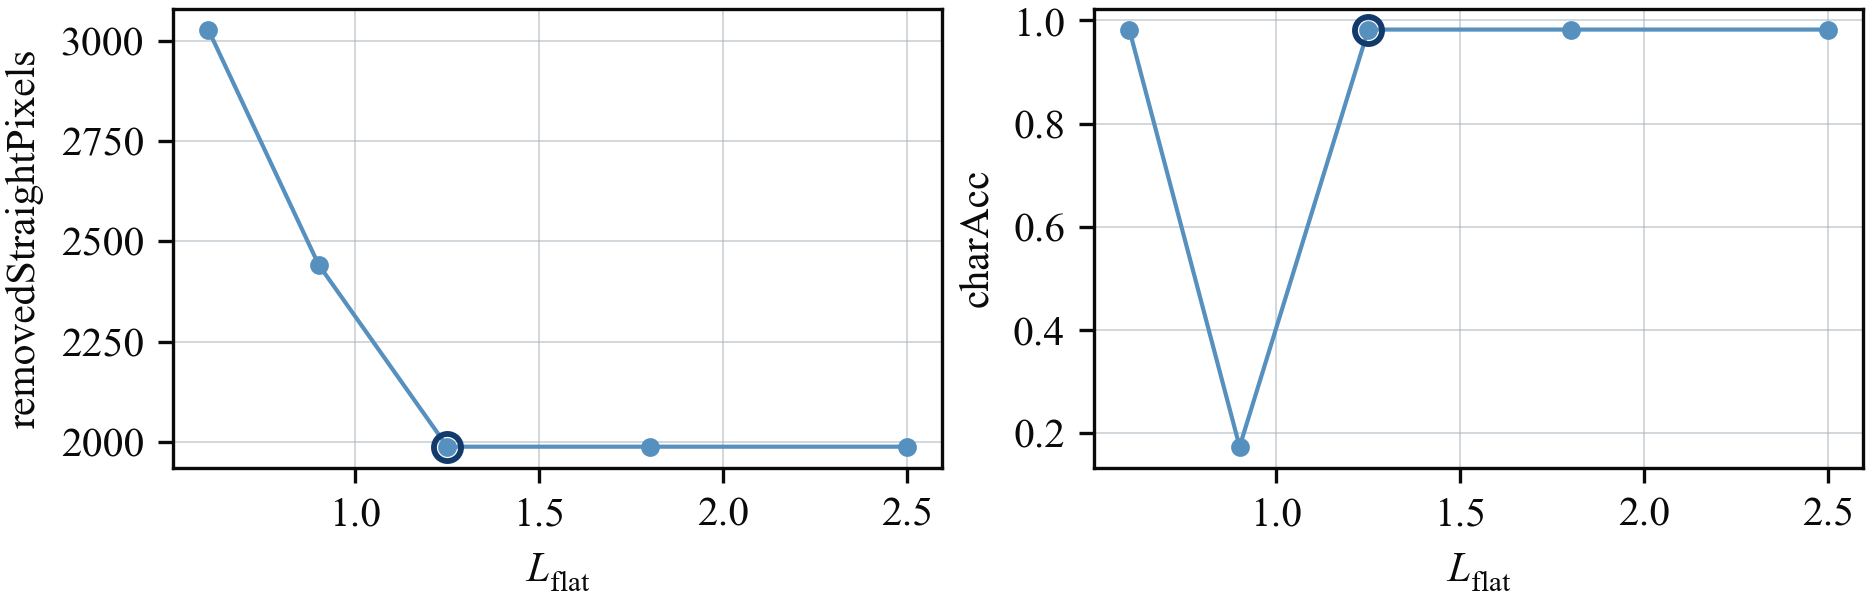
\includegraphics[width=\linewidth]{../figures/rule_flat_len_trend.png}

\caption{Length above which a flat run on the page is printed structure: measured quantities against the swept value. The circled point is the submitted value.}

\end{figure}

\begin{table}[htbp]
\centering
\small
\caption{Length above which a flat run on the page is printed structure: measured effect of each swept value. The submitted value is in bold.}
\begin{tabular}{lrrrr}
\toprule
\$L\_\{\textbackslash\{\}text\{flat\}\}\$ & \textsf{removedStraightPixels} & \textsf{nLines} & \textsf{charAcc} & \textsf{pitch} \\
\midrule
0.6 & 3028 & 20 & 0.9823 & 51 \\
0.9 & 2442 & 21 & 0.1728 & 51 \\
\bfseries 1.25 & \bfseries 1988 & \bfseries 20 & \bfseries 0.9823 & \bfseries 51 \\
1.8 & 1988 & 20 & 0.9823 & 51 \\
2.5 & 1988 & 20 & 0.9823 & 51 \\
\bottomrule
\end{tabular}
\end{table}

\subsection{Length above which an upright run on the page is printed structure}

\label{coef:rule-upright-len}

\begin{description}[leftmargin=5.2em,style=sameline]

\item[Symbol] $L_{\text{up}}$

\item[Value] \texttt{1.4}

\item[Source] \texttt{segment.py}, \texttt{RemovePrintedStructure}

\item[Swept] \texttt{0.7}, \texttt{1.0}, \texttt{1.4}, \texttt{2.0}, \texttt{2.8}

\end{description}

\paragraph{Basis}

As for the flat limit: long-run structure removal \cite{haralick1987,shafait2008}.

\paragraph{Why this value}

The vertical counterpart catches a margin rule, a spiral binding edge or the fold shadow down a page. The limit is larger than the horizontal one because tall pen strokes are more common than long flat ones: an ascender plus descender through one line already reaches most of a pitch, and two lines of writing whose ascenders and descenders touch can reach beyond it. $1.4P$ is above that worst case, so a stroke must cross nearly a line and a half before it is treated as structure. The horizontal dilation radius of $3$ before the run test tolerates a rule that wavers by a few pixels across the page.

\paragraph{What the coefficient does}

This is the more dangerous of the two limits, because a descender from one line meeting an ascender from the next makes a genuinely long vertical run of real ink. The asymmetry between $1.25$ and $1.4$ is exactly that risk difference.

\paragraph{Alternatives considered}

Deskewing first and then removing exactly vertical runs, which this code does do, or a component-level aspect-ratio test, which \texttt{DropArtifactPieces} applies afterwards as a second net.

\paragraph{Worked example}

At $P = 51$ px, $1.4P = 71$ px, against an x-height of about $21$ px at half resolution: a mark must be over three x-heights tall and under about seven pixels wide to be removed.

\paragraph{What the sweep actually showed}

This sweep produced the one result in the segmentation group where a non-submitted value scored better, and it is reported as it stands. At $L_{\text{up}} = 0.7$ the upright removal takes $4\,322$ pixels instead of $1\,988$ and reading accuracy is $0.9845$ against $0.9823$ --- better by $0.0022$, which is about one character in the eight lines scored. Two cautions. The difference is within the noise of a single page, and a more aggressive upright removal is exactly the setting that risks deleting an ascender-plus-descender column of real writing on a page where two lines interlock, which this page does not test. It is not a reason to change the submitted value on this evidence, but it is a reason to test $L_{\text{up}}$ across the whole dataset before defending $1.4$ as tuned.

\begin{figure}[htbp]

\centering

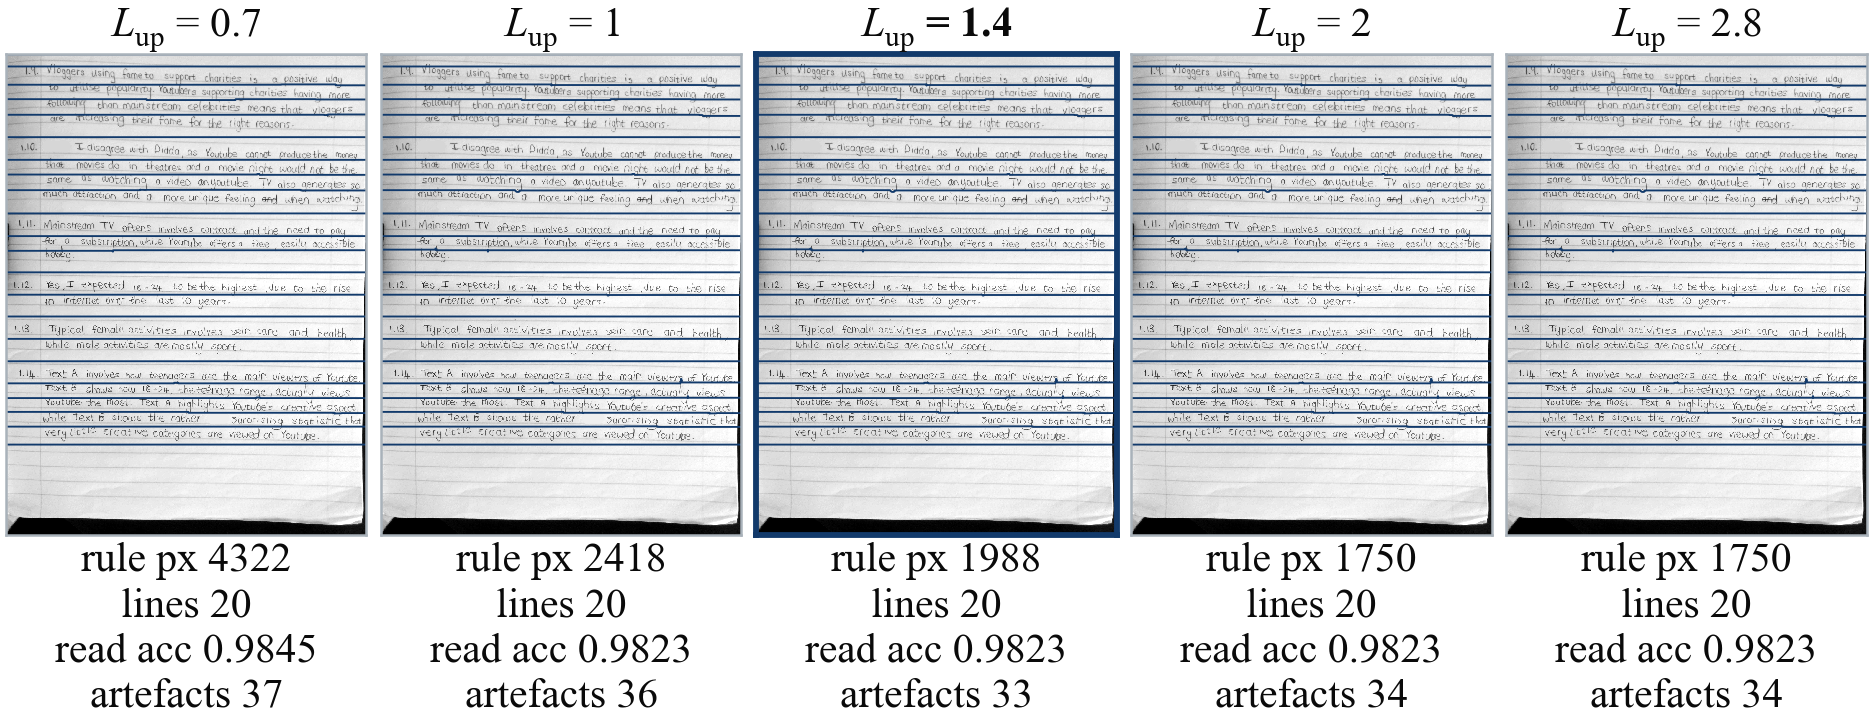
\includegraphics[width=\linewidth]{../figures/rule_upright_len.png}

\caption{Length above which an upright run on the page is printed structure. Each panel is the same input processed by the submitted code with only $L_{\text{up}}$ changed; the panel outlined in dark blue is the submitted value.}

\label{fig:rule-upright-len}

\end{figure}

\begin{figure}[htbp]

\centering

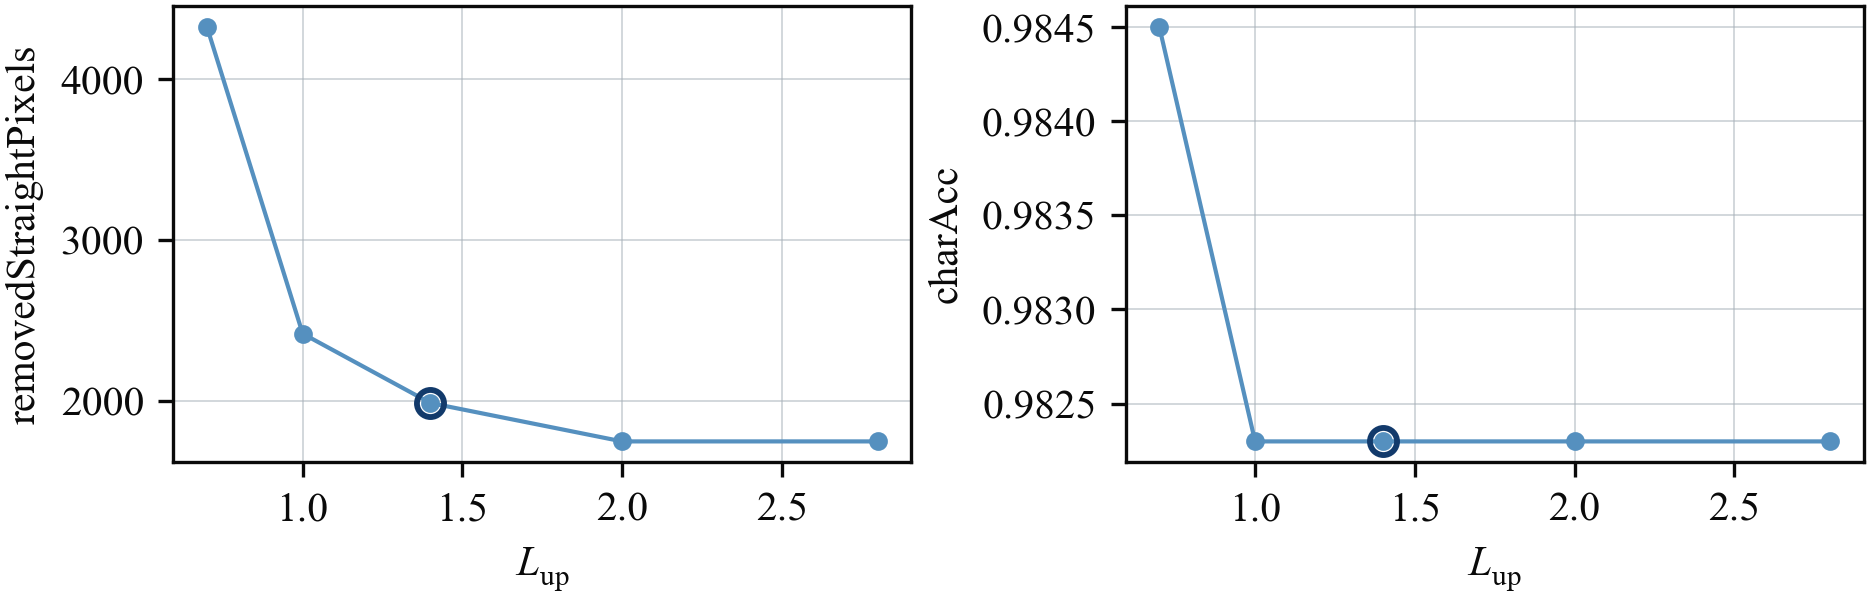
\includegraphics[width=\linewidth]{../figures/rule_upright_len_trend.png}

\caption{Length above which an upright run on the page is printed structure: measured quantities against the swept value. The circled point is the submitted value.}

\end{figure}

\begin{table}[htbp]
\centering
\small
\caption{Length above which an upright run on the page is printed structure: measured effect of each swept value. The submitted value is in bold.}
\begin{tabular}{lrrrr}
\toprule
\$L\_\{\textbackslash\{\}text\{up\}\}\$ & \textsf{removedStraightPixels} & \textsf{nLines} & \textsf{charAcc} & \textsf{artifactPieces} \\
\midrule
0.7 & 4322 & 20 & 0.9845 & 37 \\
1 & 2418 & 20 & 0.9823 & 36 \\
\bfseries 1.4 & \bfseries 1988 & \bfseries 20 & \bfseries 0.9823 & \bfseries 33 \\
2 & 1750 & 20 & 0.9823 & 34 \\
2.8 & 1750 & 20 & 0.9823 & 34 \\
\bottomrule
\end{tabular}
\end{table}

\section{Seam cutting}

\subsection{Weight on ink in the seam cost field}

\label{coef:seam-ink-weight}

\begin{description}[leftmargin=5.2em,style=sameline]

\item[Symbol] $w_{\text{ink}}$

\item[Value] \texttt{4.0}

\item[Source] \texttt{segment.py}, \texttt{SeamCuts}

\item[Swept] \texttt{1.0}, \texttt{2.0}, \texttt{4.0}, \texttt{8.0}, \texttt{16.0}

\end{description}

\paragraph{Basis}

A least-cost path cut through a cost field is seam carving \cite[10:3]{avidan2007}; applying it between text lines so the cut goes around descenders rather than through them is the standard handwritten line-separation use \cite{arvanitopoulos2014}.

\paragraph{Why this value}

The seam between two lines must prefer to pass through white paper and only cross ink when it has no choice. The cost at a pixel is $w_{\text{ink}}\,m + 0.012\,((y-\text{mid})/\text{halfGap})^2$, so $w_{\text{ink}}$ is the price of cutting one ink pixel measured against the price of wandering away from the midline. The two terms are deliberately far apart in scale: $4.0$ against a quadratic that reaches only $0.012$ at the full half-gap. One ink pixel therefore costs the same as about $333$ pixel-rows of maximum drift, which is the statement \enquote{go round the descender, however far round you must go}.

\paragraph{What the coefficient does}

Only the \emph{ratio} of the three coefficients matters, not their absolute size, since the path that minimises the total is unchanged by a common factor. Raising $w_{\text{ink}}$ makes the seam ever more willing to detour; lowering it lets the seam take a straighter path and slice through descenders, which gives the line below a stray mark and the line above a truncated letter.

\paragraph{Alternatives considered}

A straight horizontal cut at the midpoint, which is what most simple profile segmenters do and which cuts every descender; or the $A^*$ path of \cite{arvanitopoulos2014}, which is the same idea with a different search.

\paragraph{Worked example}

On the probe page the seam runs over $2448/2 = 1224$ columns with $\text{step} = 7$, so each column may move up to seven rows and the straightness penalty for the largest move is $0.02\times7 = 0.14$, still far under the $4.0$ cost of one ink pixel.

\paragraph{Earlier evidence}

An eight-setting, 48-run sensitivity study of this field was recorded earlier in \texttt{Evidence/coefficient\_sensitivity.json}; it varied the midpoint and movement penalties separately on six preselected gaps and found two raw-ink intersections retained at every setting. That study did not establish a unique optimum, and neither does this sweep.

\paragraph{What the sweep actually showed}

\textbf{No measured effect on this page}: $20$ lines and $0.9823$ reading accuracy at every value from $1.0$ to $16.0$, a sixteen-fold range. The reason is the page, not the coefficient. Owen writes at pitch $51$ px with clear gaps, so the seam has unobstructed paper between every pair of lines and the ink term is never actually traded against the others. This coefficient is re-run on a denser page in section~\ref{coef:seam-ink-weight-dense}, which is where it can be seen to do anything.

\begin{figure}[htbp]

\centering

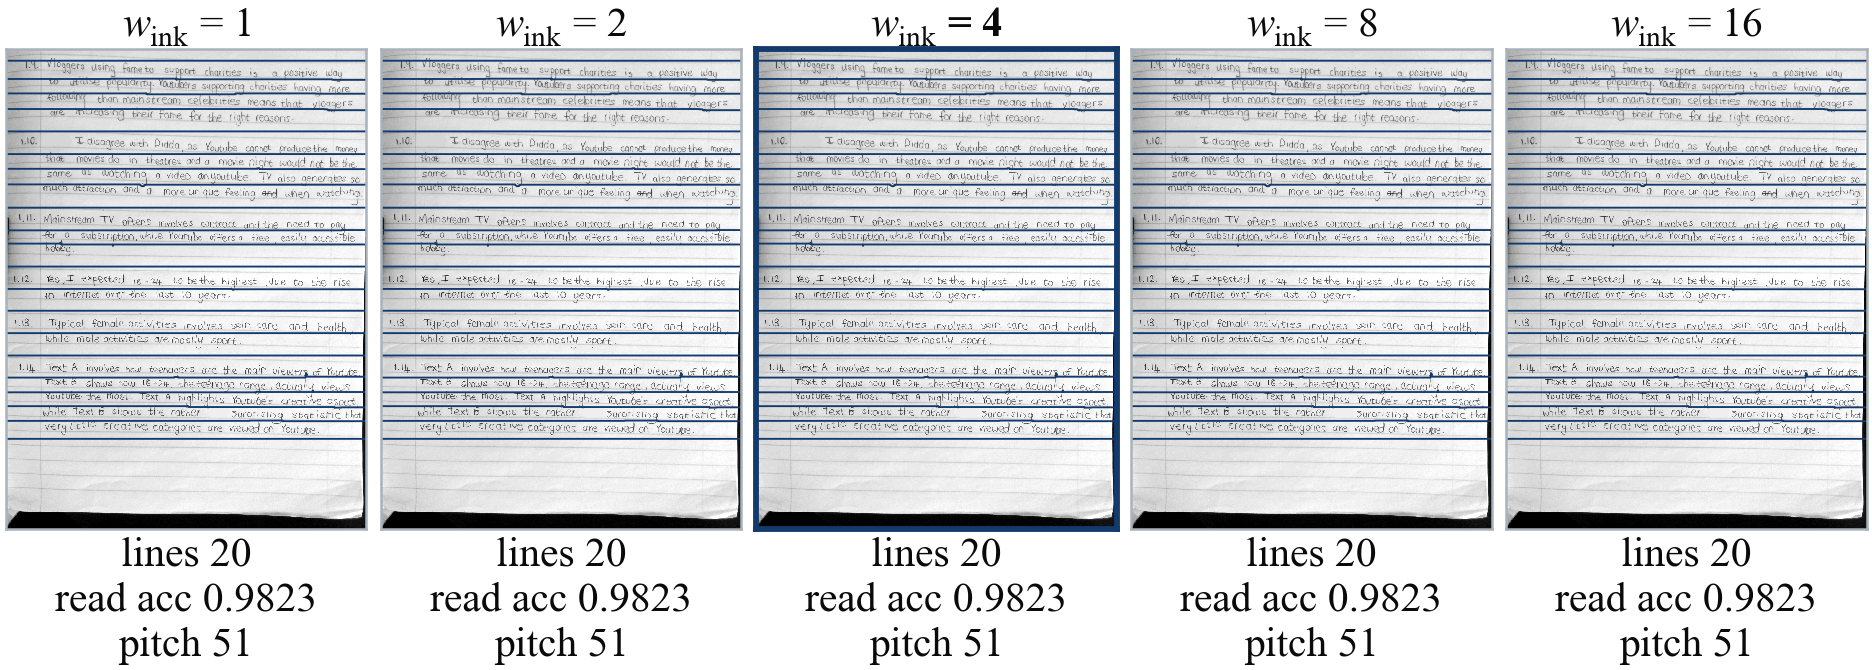
\includegraphics[width=\linewidth]{../figures/seam_ink_weight.png}

\caption{Weight on ink in the seam cost field. Each panel is the same input processed by the submitted code with only $w_{\text{ink}}$ changed; the panel outlined in dark blue is the submitted value.}

\label{fig:seam-ink-weight}

\end{figure}

\begin{figure}[htbp]

\centering

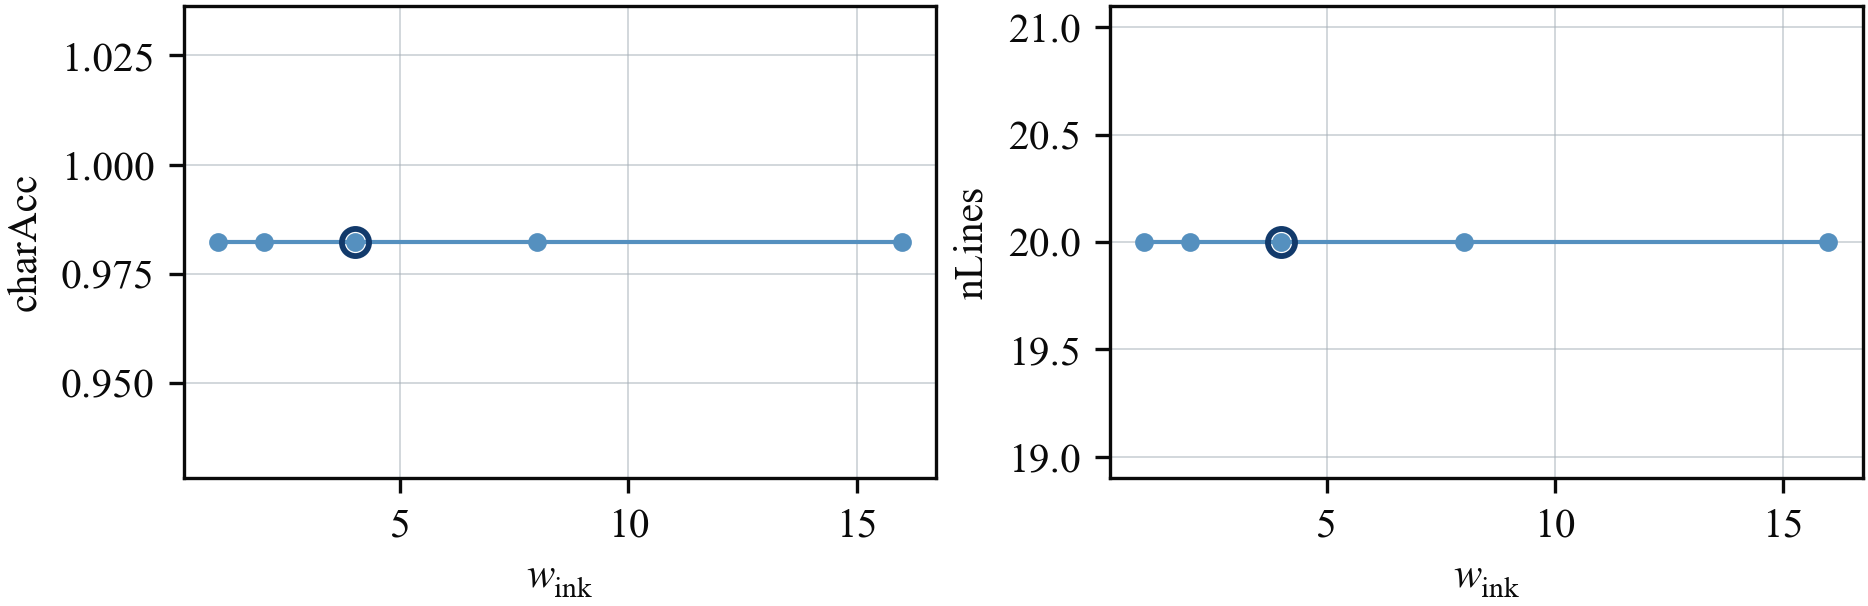
\includegraphics[width=\linewidth]{../figures/seam_ink_weight_trend.png}

\caption{Weight on ink in the seam cost field: measured quantities against the swept value. The circled point is the submitted value.}

\end{figure}

\begin{table}[htbp]
\centering
\small
\caption{Weight on ink in the seam cost field: measured effect of each swept value. The submitted value is in bold.}
\begin{tabular}{lrrr}
\toprule
\$w\_\{\textbackslash\{\}text\{ink\}\}\$ & \textsf{nLines} & \textsf{charAcc} & \textsf{pitch} \\
\midrule
1 & 20 & 0.9823 & 51 \\
2 & 20 & 0.9823 & 51 \\
\bfseries 4 & \bfseries 20 & \bfseries 0.9823 & \bfseries 51 \\
8 & 20 & 0.9823 & 51 \\
16 & 20 & 0.9823 & 51 \\
\bottomrule
\end{tabular}
\end{table}

\subsection{Weight pulling the seam back towards the midline}

\label{coef:seam-midline-pull}

\begin{description}[leftmargin=5.2em,style=sameline]

\item[Symbol] $w_{\text{mid}}$

\item[Value] \texttt{0.012}

\item[Source] \texttt{segment.py}, \texttt{SeamCuts}

\item[Swept] \texttt{0.0}, \texttt{0.004}, \texttt{0.012}, \texttt{0.05}, \texttt{0.25}

\end{description}

\paragraph{Basis}

A regularising term added to a seam cost to keep the path near a prior is the usual way to stop a minimum-cost path degenerating \cite{avidan2007,arvanitopoulos2014}.

\paragraph{Why this value}

Between two lines there is usually a wide band of clean paper, and every path through it costs the same. Without a tie-breaker the seam is then decided by floating-point accidents and can hug one line for a whole page. The quadratic term makes the midline the cheapest of those equal-cost paths while remaining negligible against real ink. It is quadratic, not linear, so it is almost free near the middle and grows only as the seam approaches a line.

\paragraph{What the coefficient does}

At $0$ the seam is unconstrained in open paper. Raised far enough it dominates the ink term and the seam becomes a straight line through the midpoint, cutting descenders: at $0.25$ the full-drift penalty is $0.25$ against $4.0$ for one ink pixel, so the seam will cross ink rather than drift more than about $16$ pixel-rows.

\paragraph{Alternatives considered}

Clamping the seam to a corridor around the midline, which is harder in that it forbids the large excursion a long descender needs, or no tie-breaker at all.

\paragraph{Worked example}

At the half-gap, $((y-\text{mid})/\text{halfGap})^2 = 1$ and the penalty is $0.012$, which is $0.3\%$ of the cost of one ink pixel.

\paragraph{What the sweep actually showed}

\textbf{No measured effect on this page}, for the same reason as the ink weight: with clean paper between the lines the seam has a wide corridor and the tie-breaker never has to break a tie that matters. The coefficient's purpose --- stopping the seam wandering arbitrarily through open paper --- is a determinism argument rather than an accuracy one, and this sweep neither confirms nor refutes it.

\begin{figure}[htbp]

\centering

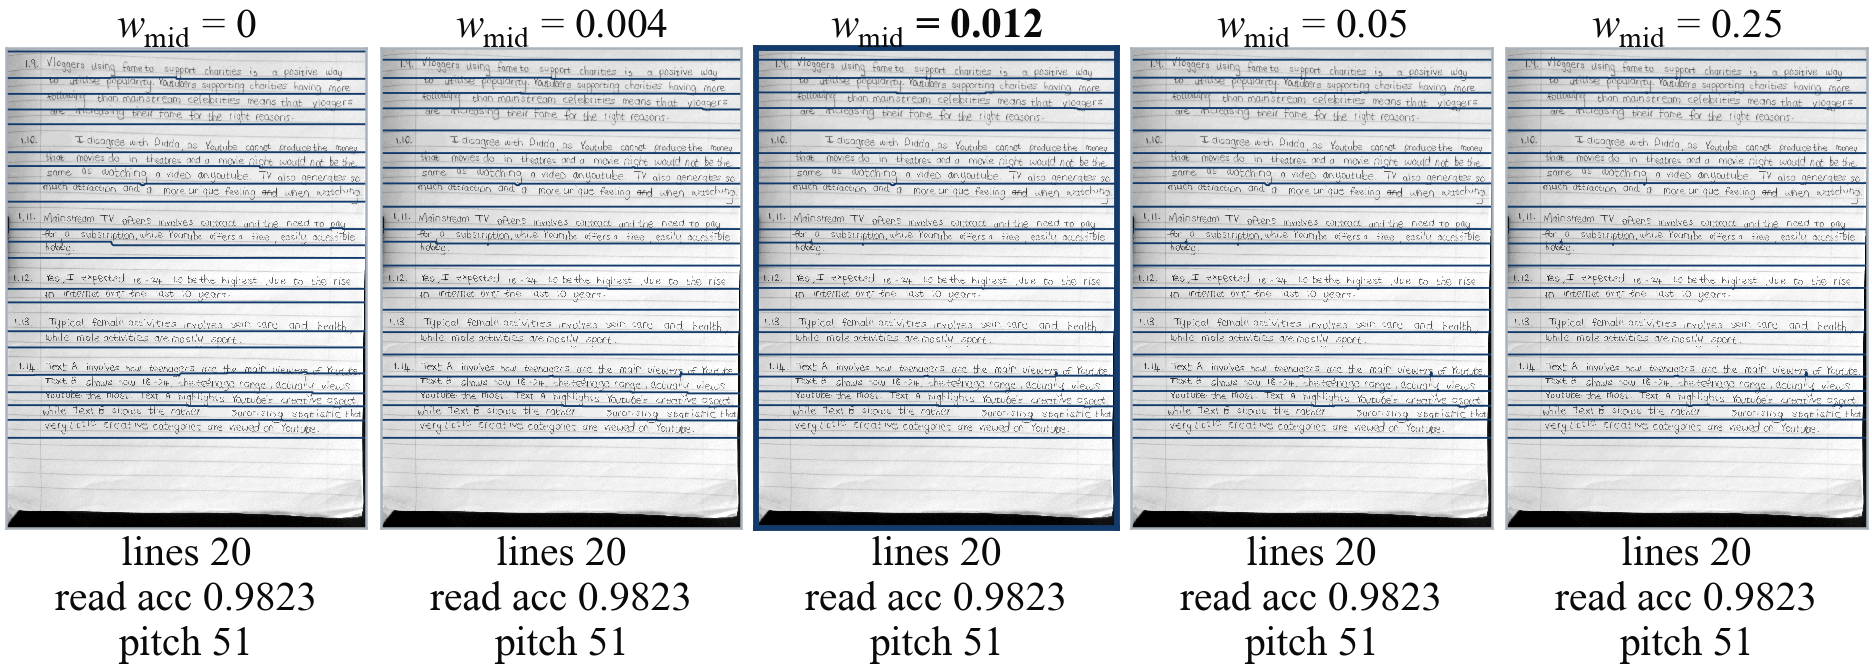
\includegraphics[width=\linewidth]{../figures/seam_midline_pull.png}

\caption{Weight pulling the seam back towards the midline. Each panel is the same input processed by the submitted code with only $w_{\text{mid}}$ changed; the panel outlined in dark blue is the submitted value.}

\label{fig:seam-midline-pull}

\end{figure}

\begin{figure}[htbp]

\centering

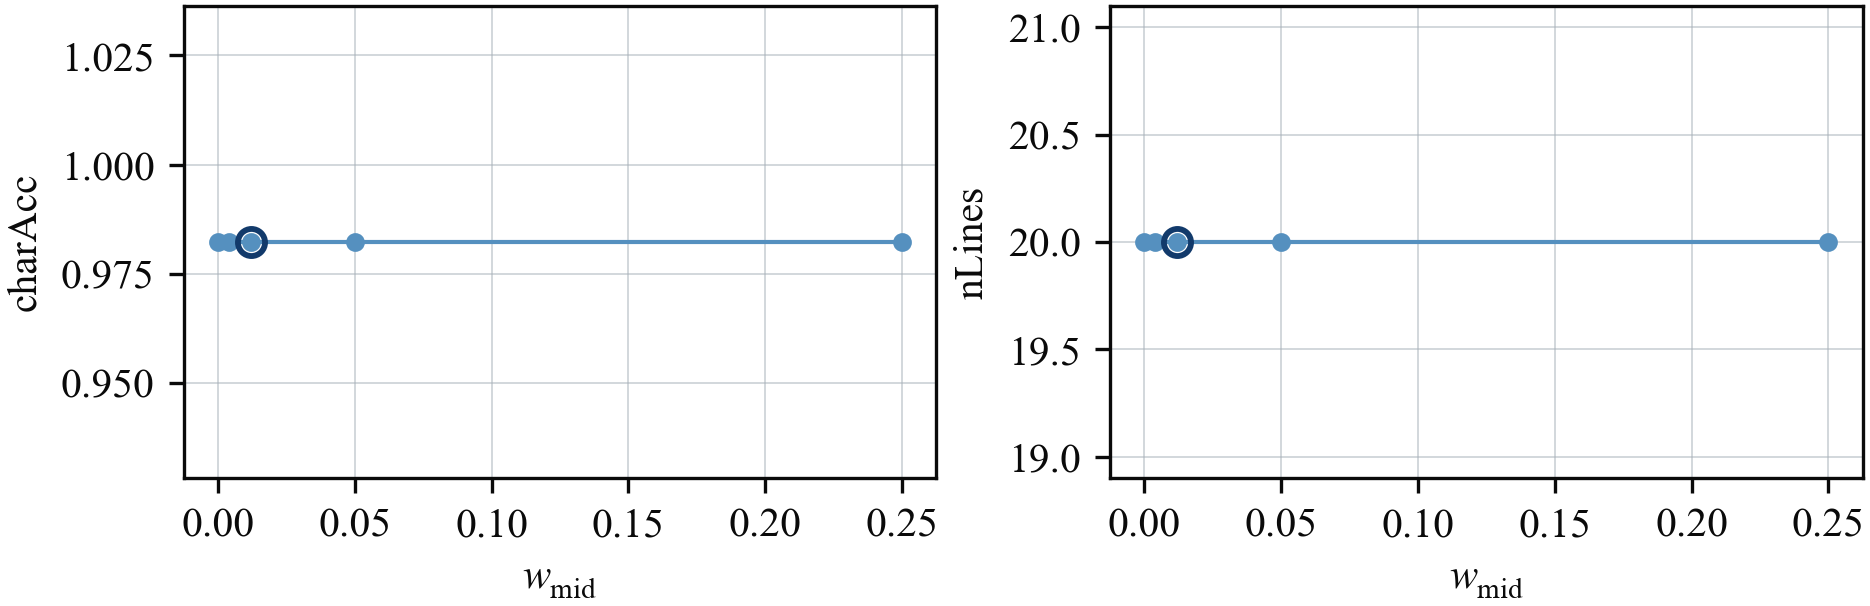
\includegraphics[width=\linewidth]{../figures/seam_midline_pull_trend.png}

\caption{Weight pulling the seam back towards the midline: measured quantities against the swept value. The circled point is the submitted value.}

\end{figure}

\begin{table}[htbp]
\centering
\small
\caption{Weight pulling the seam back towards the midline: measured effect of each swept value. The submitted value is in bold.}
\begin{tabular}{lrrr}
\toprule
\$w\_\{\textbackslash\{\}text\{mid\}\}\$ & \textsf{nLines} & \textsf{charAcc} & \textsf{pitch} \\
\midrule
0 & 20 & 0.9823 & 51 \\
0.004 & 20 & 0.9823 & 51 \\
\bfseries 0.012 & \bfseries 20 & \bfseries 0.9823 & \bfseries 51 \\
0.05 & 20 & 0.9823 & 51 \\
0.25 & 20 & 0.9823 & 51 \\
\bottomrule
\end{tabular}
\end{table}

\subsection{Rows a seam may move between adjacent columns}

\label{coef:seam-step}

\begin{description}[leftmargin=5.2em,style=sameline]

\item[Symbol] $\Delta_{\max}$

\item[Value] \texttt{7}

\item[Source] \texttt{segment.py}, \texttt{SeamCuts}

\item[Swept] \texttt{1}, \texttt{3}, \texttt{7}, \texttt{12}, \texttt{20}

\end{description}

\paragraph{Basis}

The connectivity of the seam, how far it may shift per column, is a parameter of seam carving \cite[10:3]{avidan2007}; the classical version allows one row per column.

\paragraph{Why this value}

A seam that may only move one row per column, as in the original seam carving, cannot climb around a long descender within the width of one letter: it needs the gradient to be gentle. Handwritten descenders are steep, so the step is widened to seven rows. The cost of that freedom is paid twice: the search is $O(W\,h\,(2\Delta+1))$, so time grows linearly in $\Delta$, and a large step lets the seam jump so abruptly that it no longer looks like a cut between two lines.

\paragraph{What the coefficient does}

$\Delta_{\max}$ interacts with the straightness penalty: each row of movement costs $0.02$, so the largest move costs $0.02\Delta$. At $\Delta = 7$ that is $0.14$, still cheap against ink, so the limit rather than the penalty is what binds.

\paragraph{Alternatives considered}

Four-connectivity with an unlimited number of vertical moves per column, which needs a different dynamic program, or cutting on a downsampled page and upsampling the seam.

\paragraph{Worked example}

With $\Delta = 7$ the seam can cross a $51$ px pitch in eight columns, about a third of an x-height of horizontal travel, which is enough to pass round the stem of a \texttt{g}.

\paragraph{What the sweep actually showed}

\textbf{No measured effect on the result, and a measurable one on the cost.} The line count and reading accuracy are identical at every value from $1$ to $20$, but the recorded wall time rises from about $53$ to about $69$ seconds, consistent with the search being linear in $2\Delta+1$. So on this page the extra freedom is bought and not used. It is bought for pages where a descender must be climbed around within the width of a letter, which this page does not contain.

\begin{figure}[htbp]

\centering

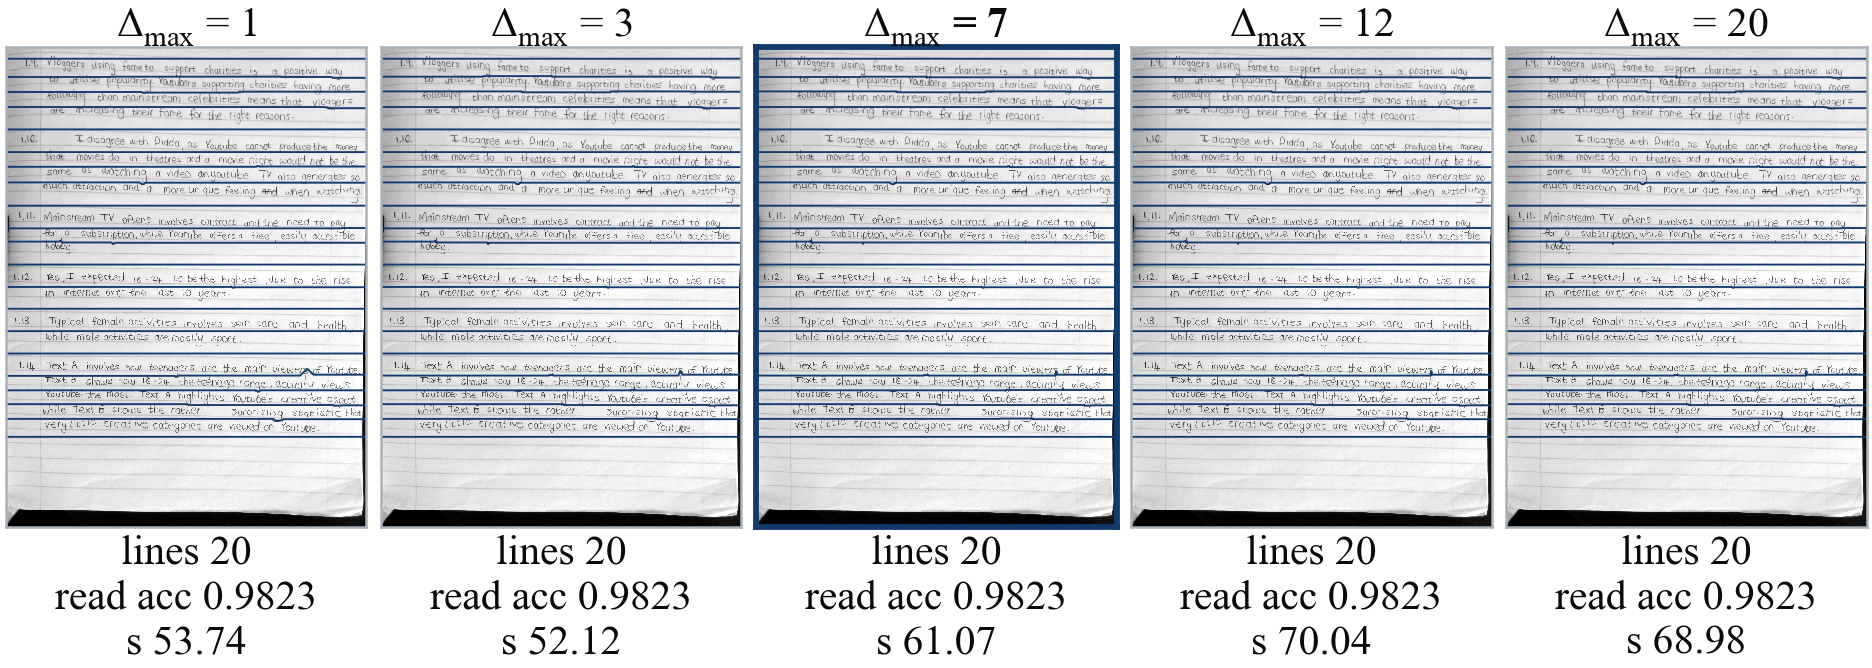
\includegraphics[width=\linewidth]{../figures/seam_step.png}

\caption{Rows a seam may move between adjacent columns. Each panel is the same input processed by the submitted code with only $\Delta_{\max}$ changed; the panel outlined in dark blue is the submitted value.}

\label{fig:seam-step}

\end{figure}

\begin{figure}[htbp]

\centering

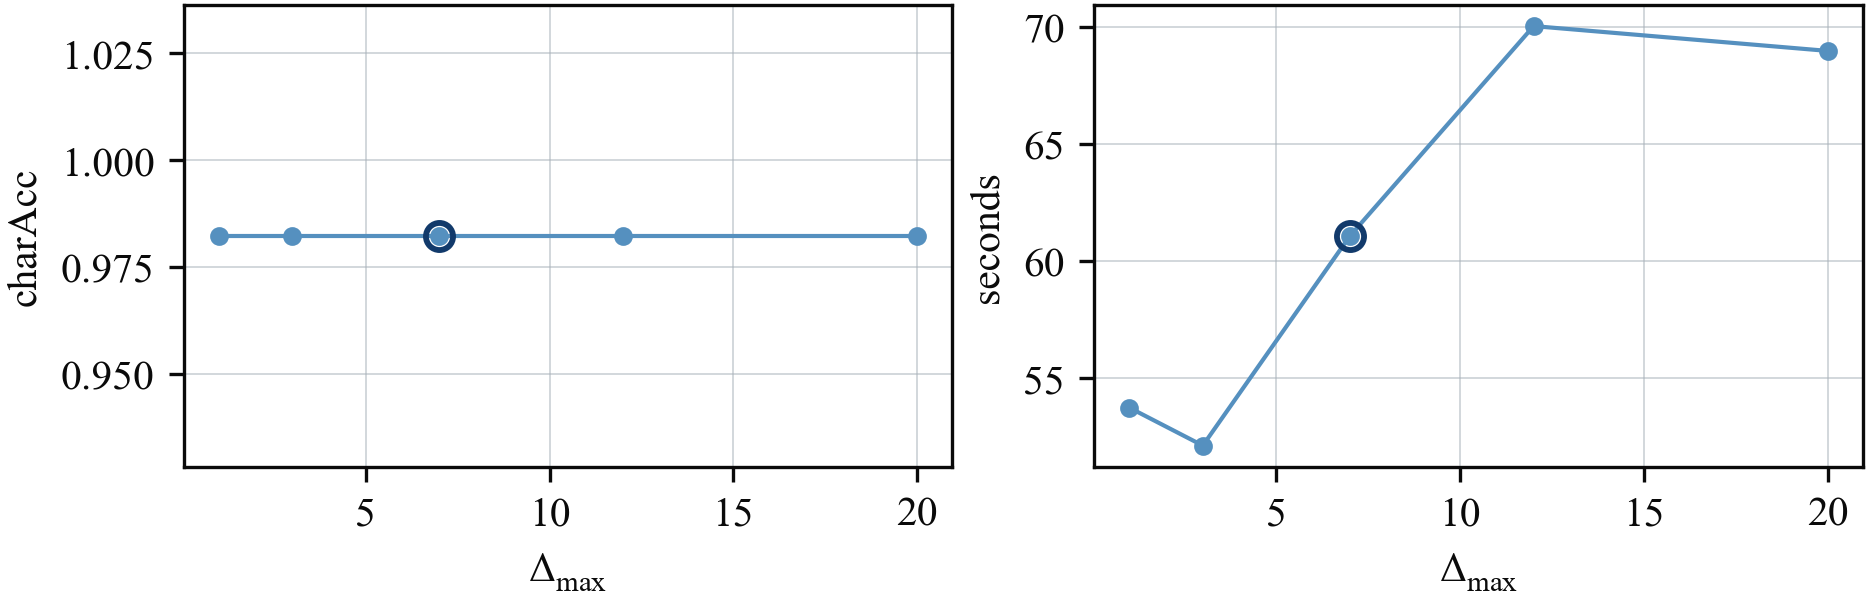
\includegraphics[width=\linewidth]{../figures/seam_step_trend.png}

\caption{Rows a seam may move between adjacent columns: measured quantities against the swept value. The circled point is the submitted value.}

\end{figure}

\begin{table}[htbp]
\centering
\small
\caption{Rows a seam may move between adjacent columns: measured effect of each swept value. The submitted value is in bold.}
\begin{tabular}{lrrr}
\toprule
\$\textbackslash\{\}Delta\_\{\textbackslash\{\}max\}\$ & \textsf{nLines} & \textsf{charAcc} & \textsf{seconds} \\
\midrule
1 & 20 & 0.9823 & 53.74 \\
3 & 20 & 0.9823 & 52.12 \\
\bfseries 7 & \bfseries 20 & \bfseries 0.9823 & \bfseries 61.07 \\
12 & 20 & 0.9823 & 70.04 \\
20 & 20 & 0.9823 & 68.98 \\
\bottomrule
\end{tabular}
\end{table}

\subsection{Closing radius applied before the seam is cut}

\label{coef:seam-tail-radius}

\begin{description}[leftmargin=5.2em,style=sameline]

\item[Symbol] $r_{\text{tail}}$

\item[Value] \texttt{0.07}

\item[Source] \texttt{segment.py}, \texttt{SeamCuts}

\item[Swept] \texttt{0.0}, \texttt{0.03}, \texttt{0.07}, \texttt{0.14}, \texttt{0.25}

\end{description}

\paragraph{Basis}

Morphological closing to suppress thin spurious passages before a path search \cite{haralick1987}.

\paragraph{Why this value}

A minimum-cost seam will find any gap, including the one-pixel channel between the two sides of a narrow loop or beside a stem. Threading such a channel splits a letter in half for no benefit. The mask is therefore closed before the cost field is built, which seals channels narrower than $r_{\text{tail}}$ while leaving the outer shape of the stroke close to real. It is a closing and not a plain dilation exactly so that the stroke does not grow.

\paragraph{What the coefficient does}

$r_{\text{tail}}$ is in line pitches, so it scales with the writing. At $0$ the seam is free to thread every gap; too large and neighbouring letters, or the descender of one line and the ascender of the next, are welded together, so the seam can no longer pass between them at all and the two lines merge.

\paragraph{Alternatives considered}

Penalising the seam for sharp vertical excursions, which the straightness term already does weakly, or post-checking each seam for how much ink it crossed.

\paragraph{Worked example}

At $P = 51$ px, $0.07P = 3.57 \to 3$, so a $3$-pixel closing: channels up to about $6$ px wide are sealed before the search.

\paragraph{What the sweep actually showed}

Four of the five values are identical and the largest, $0.25$, costs a little accuracy, $0.9801$ against $0.9823$. That is the expected direction --- an over-large closing begins to weld neighbouring ink together --- but at one character in four hundred it is weak evidence. As with the other seam coefficients, this page does not stress it; see section~\ref{coef:seam-tail-radius-dense}.

\begin{figure}[htbp]

\centering

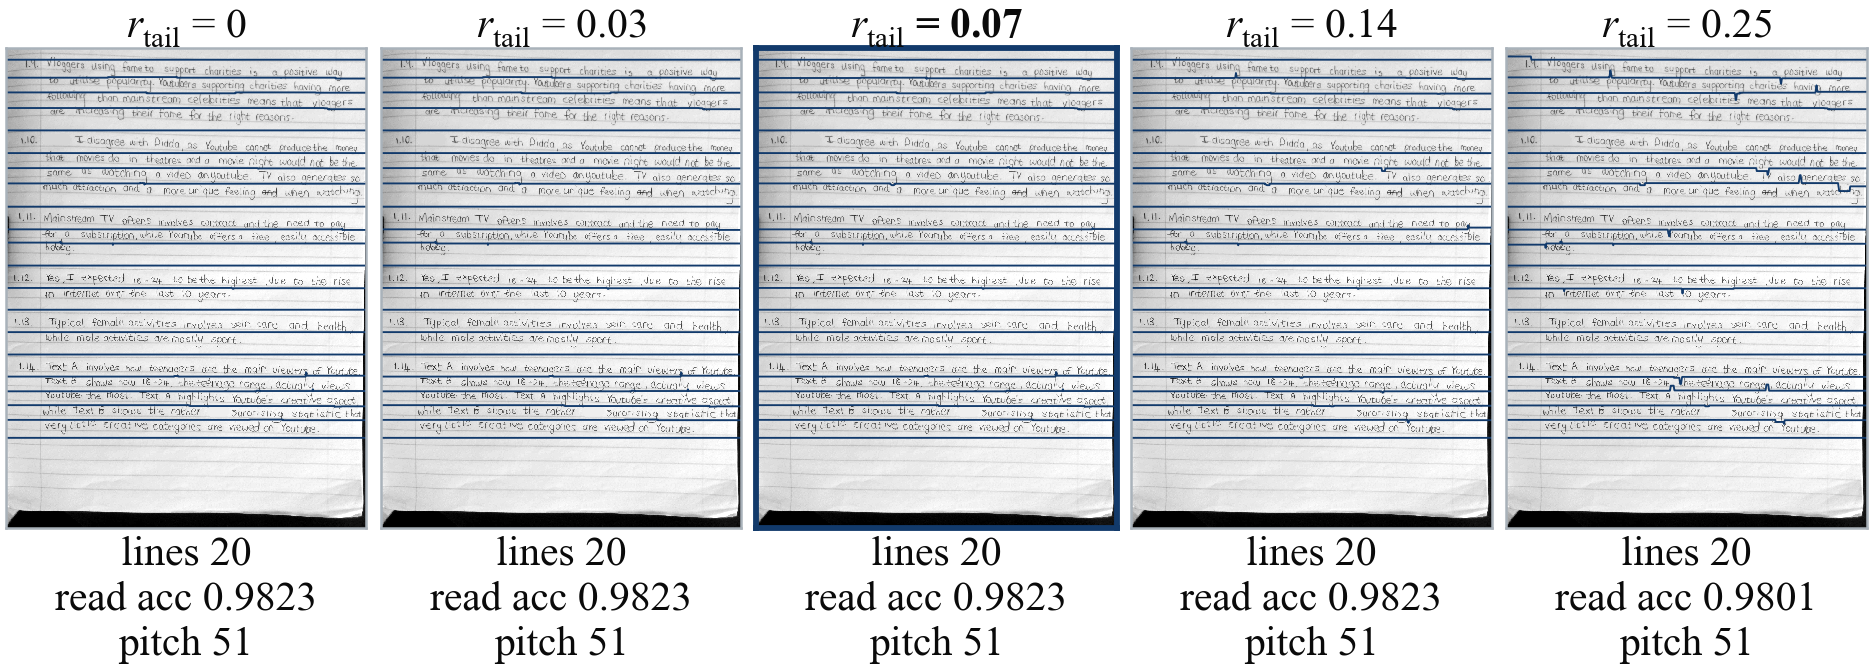
\includegraphics[width=\linewidth]{../figures/seam_tail_radius.png}

\caption{Closing radius applied before the seam is cut. Each panel is the same input processed by the submitted code with only $r_{\text{tail}}$ changed; the panel outlined in dark blue is the submitted value.}

\label{fig:seam-tail-radius}

\end{figure}

\begin{figure}[htbp]

\centering

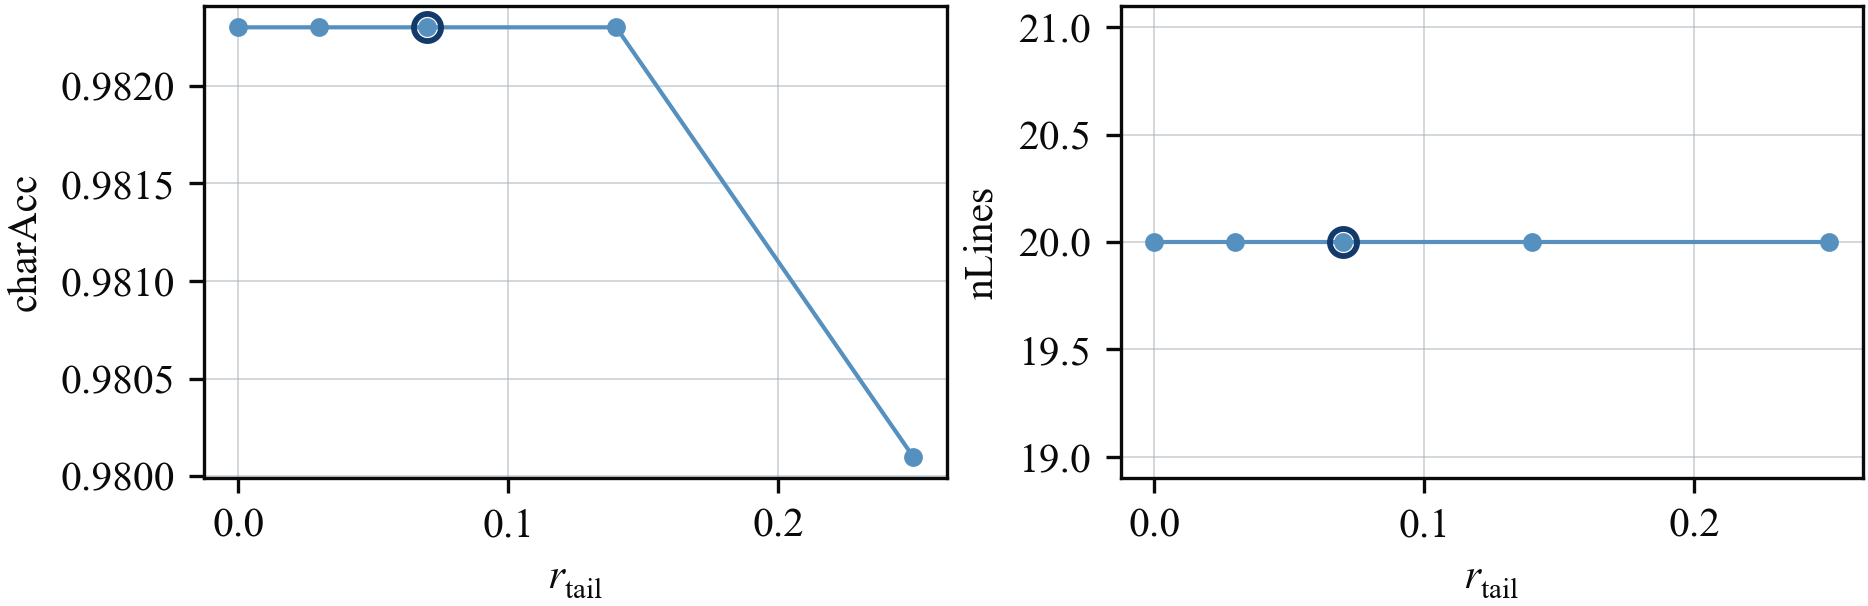
\includegraphics[width=\linewidth]{../figures/seam_tail_radius_trend.png}

\caption{Closing radius applied before the seam is cut: measured quantities against the swept value. The circled point is the submitted value.}

\end{figure}

\begin{table}[htbp]
\centering
\small
\caption{Closing radius applied before the seam is cut: measured effect of each swept value. The submitted value is in bold.}
\begin{tabular}{lrrr}
\toprule
\$r\_\{\textbackslash\{\}text\{tail\}\}\$ & \textsf{nLines} & \textsf{charAcc} & \textsf{pitch} \\
\midrule
0 & 20 & 0.9823 & 51 \\
0.03 & 20 & 0.9823 & 51 \\
\bfseries 0.07 & \bfseries 20 & \bfseries 0.9823 & \bfseries 51 \\
0.14 & 20 & 0.9823 & 51 \\
0.25 & 20 & 0.9801 & 51 \\
\bottomrule
\end{tabular}
\end{table}

\section{Line ownership}

\subsection{Share of a piece's ink that must lie in a band for it to count}

\label{coef:band-ink-share}

\begin{description}[leftmargin=5.2em,style=sameline]

\item[Symbol] $\theta_{\text{band}}$

\item[Value] \texttt{0.15}

\item[Source] \texttt{segment.py}, \texttt{\_BandOwnership}

\item[Swept] \texttt{0.05}, \texttt{0.1}, \texttt{0.15}, \texttt{0.25}, \texttt{0.4}

\end{description}

\paragraph{Basis}

Assigning a connected component to the text line holding most of it is the usual resolution step after a coarse line cut \cite{likforman2007}.

\paragraph{Why this value}

After the seams are cut, each piece of ink is scored by how much of it falls in each band. A piece is treated as genuinely present in a band if at least $\theta_{\text{band}}$ of its ink is there. The share must be low enough that a real descender, which puts only its tail into the band below, is still seen in both, and high enough that a few pixels of anti-aliased overlap do not count. A descender tail is typically a fifth to a third of the letter; a spurious overlap is a few per cent. $0.15$ lies between them.

\paragraph{What the coefficient does}

Where a piece is substantial in more than one band it is given to the \emph{topmost}, which is the rule that keeps a letter with the line it was written on rather than the line its tail reaches into. Lowering $\theta_{\text{band}}$ makes more pieces look multi-band, and because of the topmost rule that pulls ink upward; raising it makes a genuine two-line piece look single-band and it is then assigned by majority instead.

\paragraph{Alternatives considered}

Majority ownership alone, which is the \texttt{cnt.argmax} fallback already used when nothing is substantial, or assigning by the centroid of the piece, which fails for a long descender.

\paragraph{Worked example}

A piece with $300$ ink pixels is counted as present in a band once at least $45$ of them fall inside it.

\paragraph{What the sweep actually showed}

\textbf{No measured effect}: $20$ lines and $0.9823$ at every value from $0.05$ to $0.40$. Ownership is only contentious for a piece of ink that genuinely spans two bands, which needs lines close enough that descenders reach into the line below. On this page almost every piece sits wholly inside one band and the share test is never close. Re-run on a dense page in section~\ref{coef:band-ink-share-dense}.

\begin{figure}[htbp]

\centering

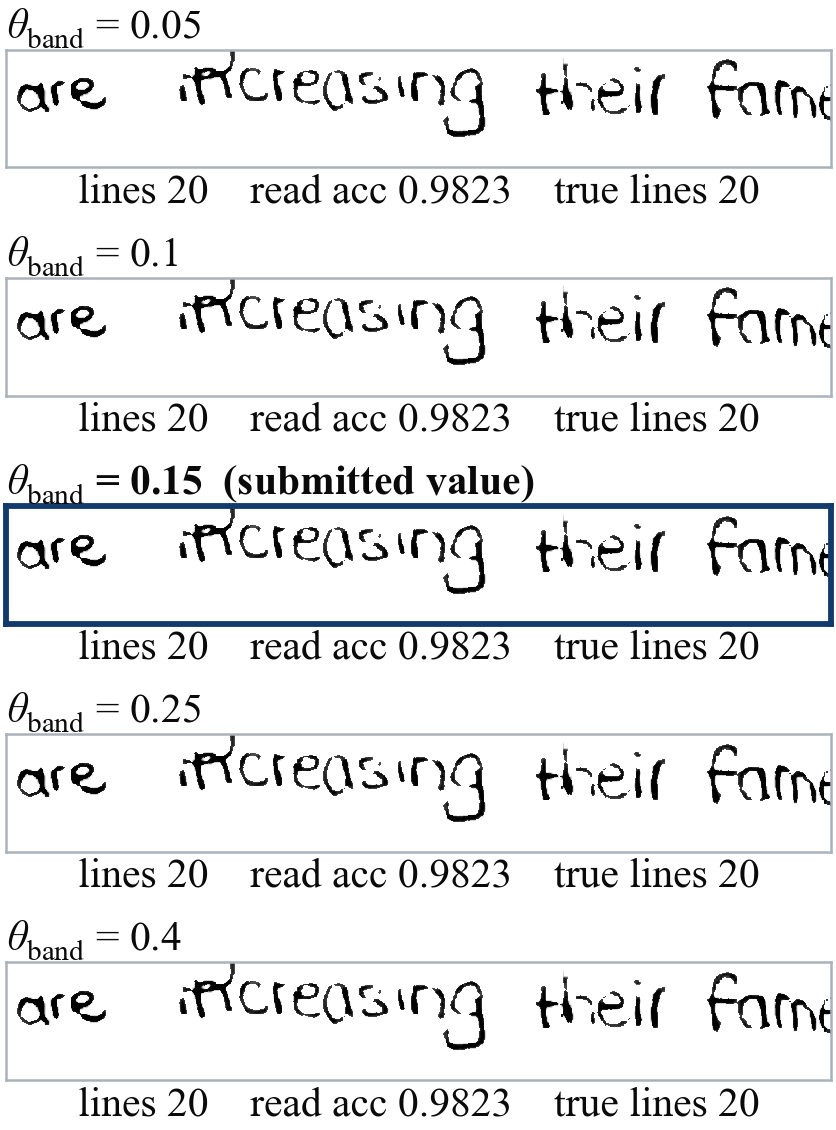
\includegraphics[width=\linewidth]{../figures/band_ink_share.png}

\caption{Share of a piece's ink that must lie in a band for it to count. Each panel is the same input processed by the submitted code with only $\theta_{\text{band}}$ changed; the panel outlined in dark blue is the submitted value.}

\label{fig:band-ink-share}

\end{figure}

\begin{figure}[htbp]

\centering

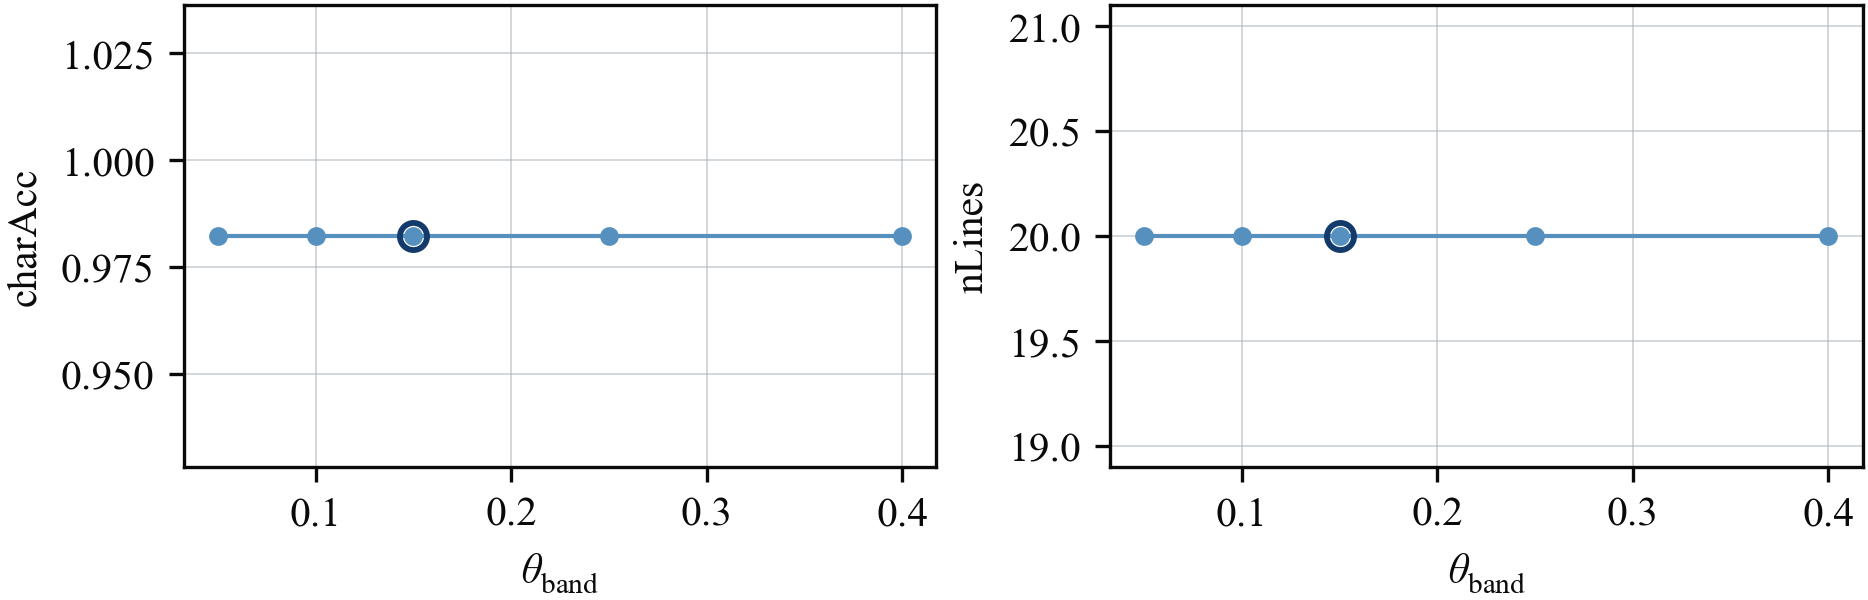
\includegraphics[width=\linewidth]{../figures/band_ink_share_trend.png}

\caption{Share of a piece's ink that must lie in a band for it to count: measured quantities against the swept value. The circled point is the submitted value.}

\end{figure}

\begin{table}[htbp]
\centering
\small
\caption{Share of a piece's ink that must lie in a band for it to count: measured effect of each swept value. The submitted value is in bold.}
\begin{tabular}{lrrr}
\toprule
\$\textbackslash\{\}theta\_\{\textbackslash\{\}text\{band\}\}\$ & \textsf{nLines} & \textsf{charAcc} & \textsf{nLinesTruth} \\
\midrule
0.05 & 20 & 0.9823 & 20 \\
0.1 & 20 & 0.9823 & 20 \\
\bfseries 0.15 & \bfseries 20 & \bfseries 0.9823 & \bfseries 20 \\
0.25 & 20 & 0.9823 & 20 \\
0.4 & 20 & 0.9823 & 20 \\
\bottomrule
\end{tabular}
\end{table}

\section{Crop building}

\subsection{Padding kept around a line crop}

\label{coef:crop-pad}

\begin{description}[leftmargin=5.2em,style=sameline]

\item[Symbol] $p_{\text{crop}}$

\item[Value] \texttt{0.15}

\item[Source] \texttt{segment.py}, \texttt{\_BuildLineCrop}

\item[Swept] \texttt{0.0}, \texttt{0.07}, \texttt{0.15}, \texttt{0.3}, \texttt{0.5}

\end{description}

\paragraph{Basis}

Leaving a margin around a text line before recognition is standard practice for CRNN line recognisers, which are trained on padded line images \cite{shi2017,puigcerver2017}.

\paragraph{Why this value}

The crop is cut to the bounding box of the ink owned by the line and then padded. Some padding is needed because the networks were trained on line images with a margin, and because a stroke that touches the edge of a crop is cut off by the resize. The padding is also what defines the left margin every crop is shifted to, so that the reader always sees writing start in the same place. Too much padding shrinks the writing once the crop is fitted to the fixed $64\times640$ canvas, because the fit preserves aspect ratio.

\paragraph{What the coefficient does}

On the fixed canvas the scale is $\min(64/h,\,640/w)$, so padding costs resolution directly: padding a $156$ px tall crop by $0.5P = 25$ px on each side makes it $206$ px tall and shrinks the writing by $24\%$ before the network sees it.

\paragraph{Alternatives considered}

No padding and relying on the canvas fit alone, or padding in x-heights rather than line pitches, which would be more faithful to the writing but needs the band measured first.

\paragraph{Worked example}

At $P = 51$ px (half resolution) the padding is $7$ px at half size, $14$ px on the full-resolution crop the writing is finally cut from.

\paragraph{What the sweep actually showed}

The result is non-monotone and the differences are tiny: $0.9797$, $0.9752$, $0.9823$, $0.9826$, $0.9757$ for padding $0$ to $0.5P$. The submitted $0.15P$ and the neighbouring $0.30P$ are within $0.0003$ of each other, which is a fraction of one character, so \textbf{this sweep does not distinguish them}. What it does show is that both extremes are worse: no padding at all clips strokes at the crop edge, and $0.5P$ shrinks the writing enough on the fixed canvas to cost accuracy. The submitted value sits inside a broad flat optimum rather than at a sharp peak, and should be described that way.

\begin{figure}[htbp]

\centering

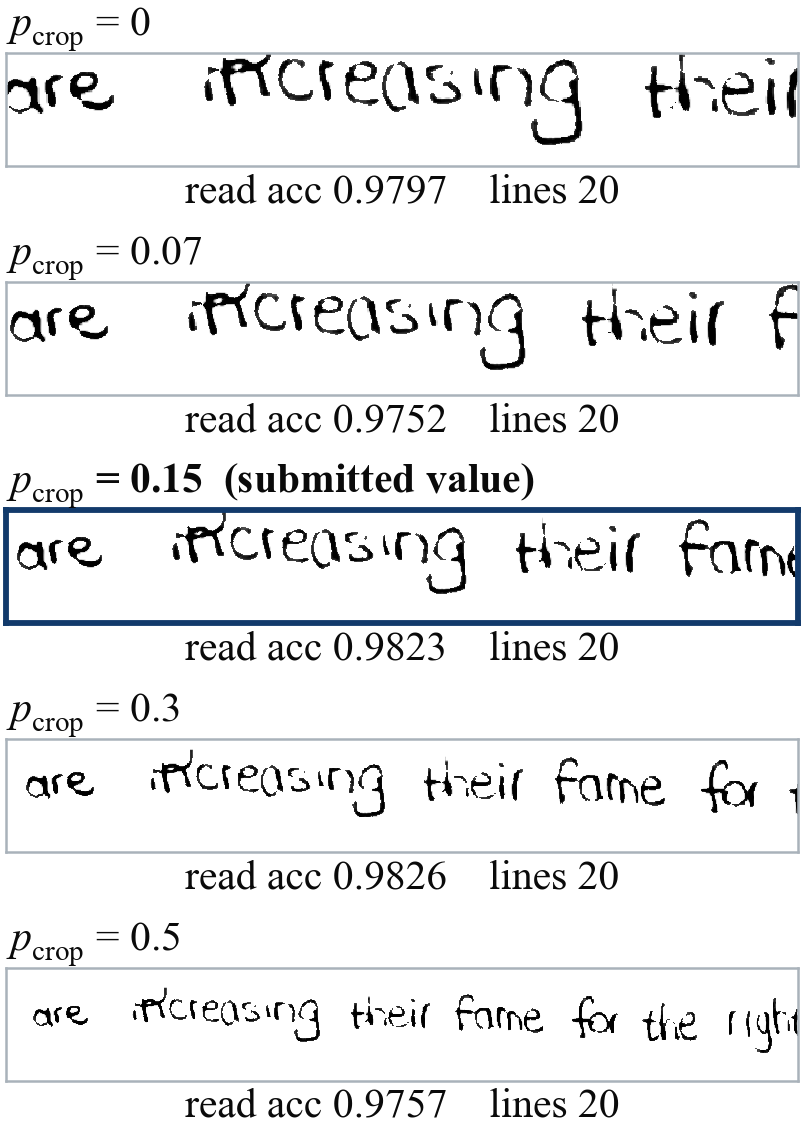
\includegraphics[width=\linewidth]{../figures/crop_pad.png}

\caption{Padding kept around a line crop. Each panel is the same input processed by the submitted code with only $p_{\text{crop}}$ changed; the panel outlined in dark blue is the submitted value.}

\label{fig:crop-pad}

\end{figure}

\begin{figure}[htbp]

\centering

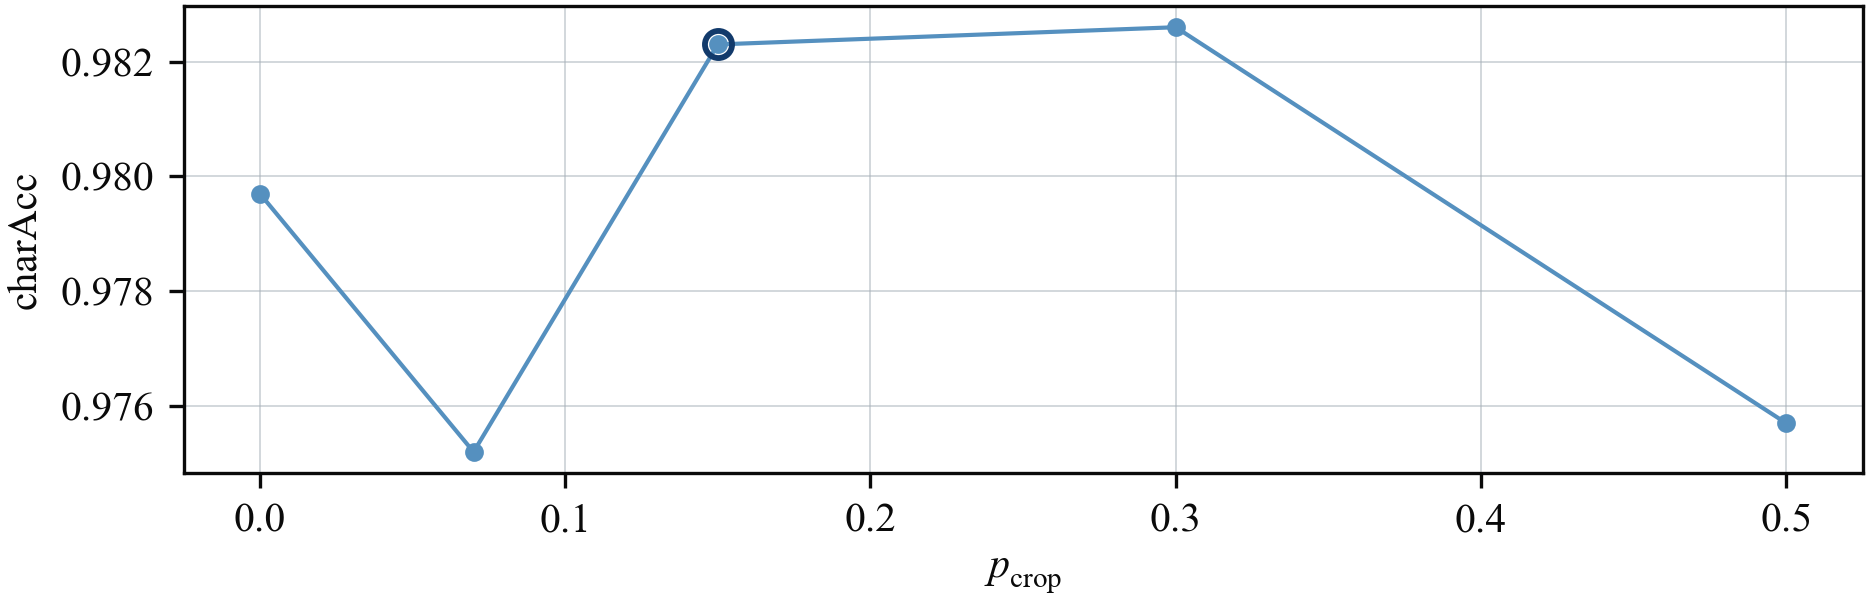
\includegraphics[width=\linewidth]{../figures/crop_pad_trend.png}

\caption{Padding kept around a line crop: measured quantities against the swept value. The circled point is the submitted value.}

\end{figure}

\begin{table}[htbp]
\centering
\small
\caption{Padding kept around a line crop: measured effect of each swept value. The submitted value is in bold.}
\begin{tabular}{lrr}
\toprule
\$p\_\{\textbackslash\{\}text\{crop\}\}\$ & \textsf{charAcc} & \textsf{nLines} \\
\midrule
0 & 0.9797 & 20 \\
0.07 & 0.9752 & 20 \\
\bfseries 0.15 & \bfseries 0.9823 & \bfseries 20 \\
0.3 & 0.9826 & 20 \\
0.5 & 0.9757 & 20 \\
\bottomrule
\end{tabular}
\end{table}

\subsection{Darkness exponent applied to a finished line crop}

\label{coef:darkness-gamma}

\begin{description}[leftmargin=5.2em,style=sameline]

\item[Symbol] $\gamma$

\item[Value] \texttt{0.55}

\item[Source] \texttt{segment.py}, \texttt{\_BuildLineCrop}

\item[Swept] \texttt{0.3}, \texttt{0.42}, \texttt{0.55}, \texttt{0.75}, \texttt{1.0}

\end{description}

\paragraph{Basis}

A power law on intensity is gamma correction, the standard tone transfer of image display \cite{itu601}; applying it to deepen faint strokes before recognition is contrast enhancement in the sense of \cite{haralick1987}.

\paragraph{Why this value}

The crop is first stretched linearly between the typical ink level (the $40$th percentile of pixels under the mask) and the paper level (the $75$th percentile of the region). That alone leaves a ballpoint stroke that skipped as a pale grey smear. Raising darkness to a power below one lifts the mid-tones without touching black or white: $0$ and $1$ are fixed points of $d^{\gamma}$, so the ink stays ink and the paper stays paper while everything between is darkened. The value has to deepen a faint stroke without turning paper texture into ink, and $0.55$ roughly doubles a mid-grey: $0.5^{0.55} = 0.68$.

\paragraph{What the coefficient does}

$\gamma = 1$ is no correction at all, which is the honest bottom of the sweep. As $\gamma$ falls, the writing thickens and faint strokes join up; past a point the paper grain in the halo also darkens and the stroke edges smear. Because the networks were trained on crops produced with $\gamma = 0.55$, moving it is a test-time mismatch as well as a visual change.

\paragraph{Alternatives considered}

Histogram equalisation, which is data-dependent and so varies between crops of the same page, or CLAHE, which adds a tile size and a clip limit of its own.

\paragraph{Worked example}

A pixel at $60\%$ darkness becomes $0.6^{0.55} = 0.76$, so a stroke at grey level $102$ is redrawn at $61$, clearly darker but not black.

\paragraph{What the sweep actually showed}

The visual effect is large and the measured effect is almost nil, and both halves of that are worth stating. The figure shows the strokes going from heavy and blotted at $\gamma = 0.30$ to pale and broken at $\gamma = 1.0$, which is a clear difference to the eye. Reading accuracy over the first eight lines is $0.9823$ at every value except $\gamma = 1.0$, where it is $0.9797$ --- a difference of one character in roughly four hundred. The honest conclusion is that on well-exposed pages the reader is robust to this correction and $\gamma$ is doing cosmetic work; its value would be tested properly on an underexposed page, where the uncorrected strokes are genuinely faint, and no such page is in this probe set.

\begin{figure}[htbp]

\centering

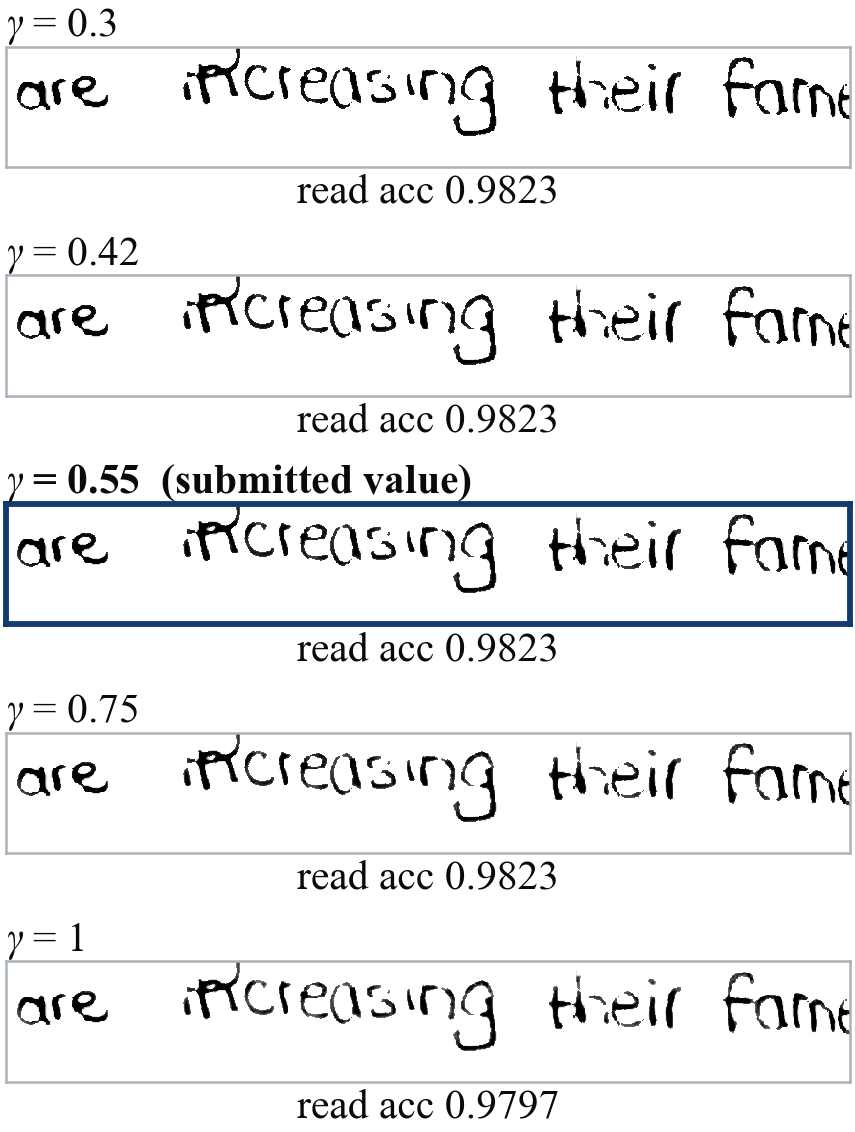
\includegraphics[width=\linewidth]{../figures/darkness_gamma.png}

\caption{Darkness exponent applied to a finished line crop. Each panel is the same input processed by the submitted code with only $\gamma$ changed; the panel outlined in dark blue is the submitted value.}

\label{fig:darkness-gamma}

\end{figure}

\begin{figure}[htbp]

\centering

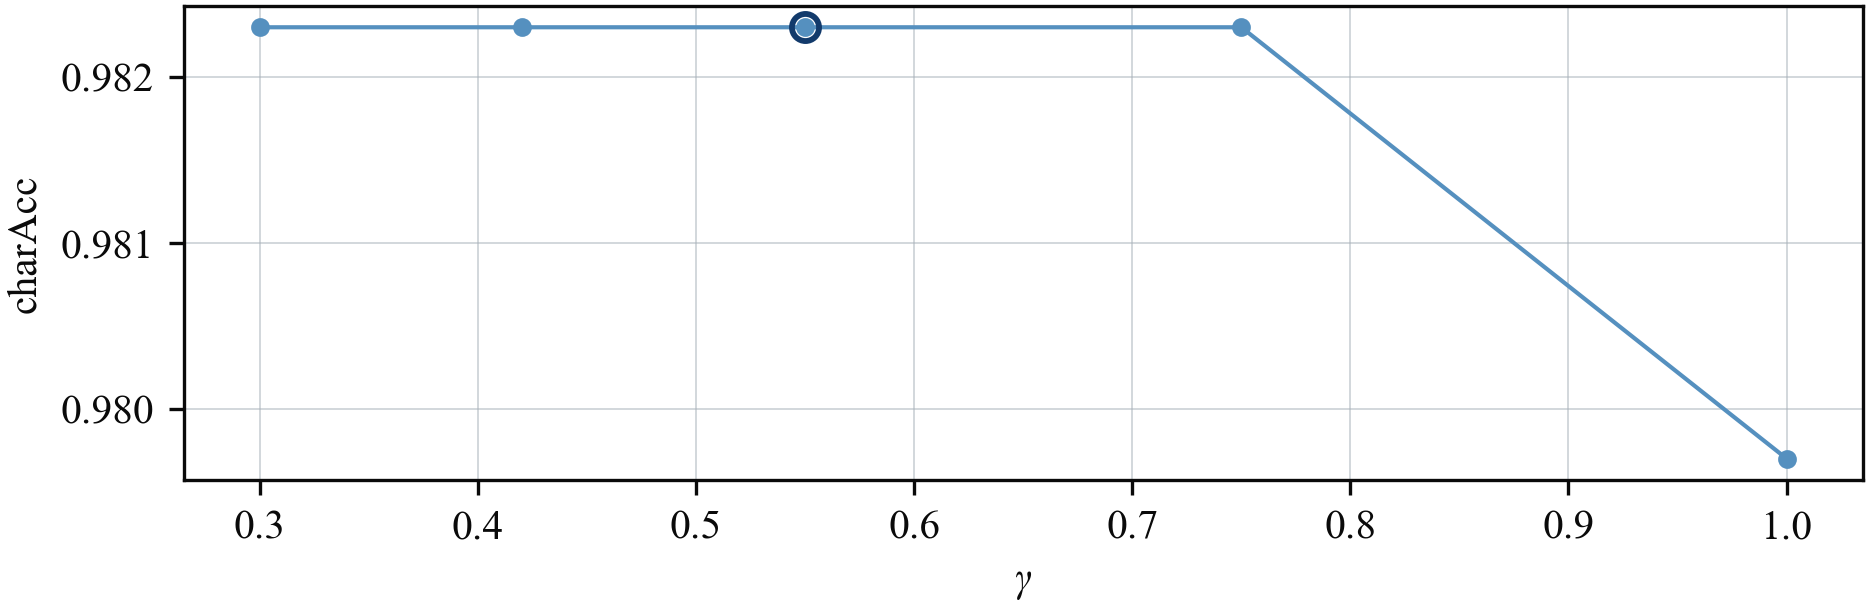
\includegraphics[width=\linewidth]{../figures/darkness_gamma_trend.png}

\caption{Darkness exponent applied to a finished line crop: measured quantities against the swept value. The circled point is the submitted value.}

\end{figure}

\begin{table}[htbp]
\centering
\small
\caption{Darkness exponent applied to a finished line crop: measured effect of each swept value. The submitted value is in bold.}
\begin{tabular}{lrr}
\toprule
\$\textbackslash\{\}gamma\$ & \textsf{charAcc} & \textsf{inkPct} \\
\midrule
0.3 & 0.9823 & [5.959, 7.186, 8.388, 7.74, 6.887, 6.159 \\
0.42 & 0.9823 & [5.956, 7.18, 8.38, 7.729, 6.879, 6.149, \\
\bfseries 0.55 & \bfseries 0.9823 & \bfseries [5.953, 7.178, 8.378, 7.726, 6.861, 6.12 \\
0.75 & 0.9823 & [5.946, 7.165, 8.374, 7.718, 6.822, 6.08 \\
1 & 0.9797 & [5.917, 7.106, 8.286, 7.651, 6.739, 6.03 \\
\bottomrule
\end{tabular}
\end{table}

\subsection{Percentile of masked pixels taken as the ink level}

\label{coef:crop-black-pct}

\begin{description}[leftmargin=5.2em,style=sameline]

\item[Symbol] $q_{\text{ink}}$

\item[Value] \texttt{40}

\item[Source] \texttt{segment.py}, \texttt{\_BuildLineCrop}

\item[Swept] \texttt{10}, \texttt{25}, \texttt{40}, \texttt{60}, \texttt{80}

\end{description}

\paragraph{Basis}

Percentile-based black and white points are the robust form of contrast stretching, preferred to the extremes because a single outlier sets those \cite{haralick1987}.

\paragraph{Why this value}

The linear stretch needs a black point. Using the darkest pixel would hand the whole stretch to one noise pixel or one blot, so a percentile of the pixels under the stroke mask is used instead. It is taken below the median on purpose: the mask includes the soft edges of the stroke, which are lighter than the core, so the median of masked pixels is already greyer than real ink. The $40$th percentile sits inside the dark core while still being a robust statistic over many pixels.

\paragraph{What the coefficient does}

Raising $q_{\text{ink}}$ takes a lighter pixel as black, so the stretch is stronger and the stroke is driven to full black with its edges, thickening the writing. Lowering it takes a darker reference, so the stretch is weaker and the crop stays flat.

\paragraph{Alternatives considered}

The mean under the mask, which the stroke edges drag up, or Otsu's threshold applied again to the masked pixels, which is another criterion where a percentile suffices.

\paragraph{Worked example}

On the probe crop the paper point is the $75$th percentile of the whole region and the ink point the $40$th of the masked pixels; the gain is $255/(\text{white}-\text{black})$.

\paragraph{What the sweep actually showed}

\textbf{No measured effect}: $0.9823$ at every percentile from $10$ to $80$. The linear stretch that follows is evidently not the binding constraint on this page --- the subsequent gamma correction and the reader's own robustness absorb the difference. The coefficient would matter on a low-contrast page; this one is well exposed.

\begin{figure}[htbp]

\centering

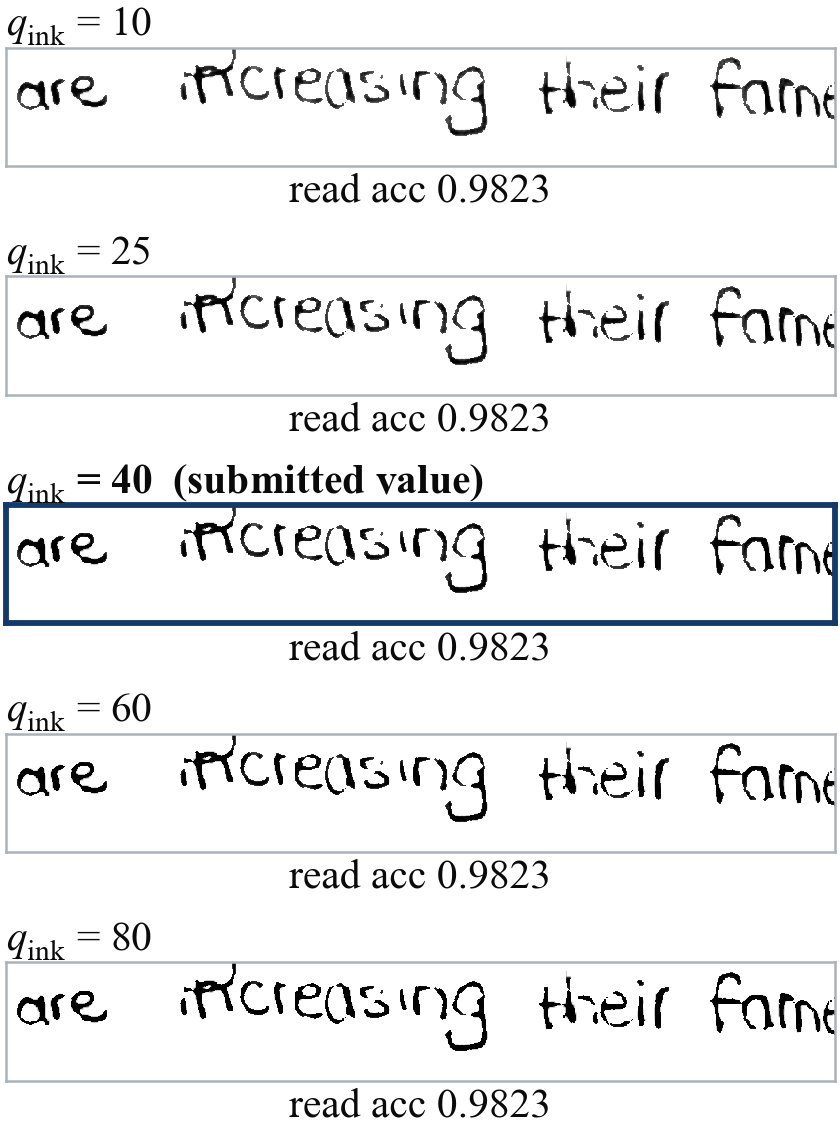
\includegraphics[width=\linewidth]{../figures/crop_black_pct.png}

\caption{Percentile of masked pixels taken as the ink level. Each panel is the same input processed by the submitted code with only $q_{\text{ink}}$ changed; the panel outlined in dark blue is the submitted value.}

\label{fig:crop-black-pct}

\end{figure}

\begin{figure}[htbp]

\centering

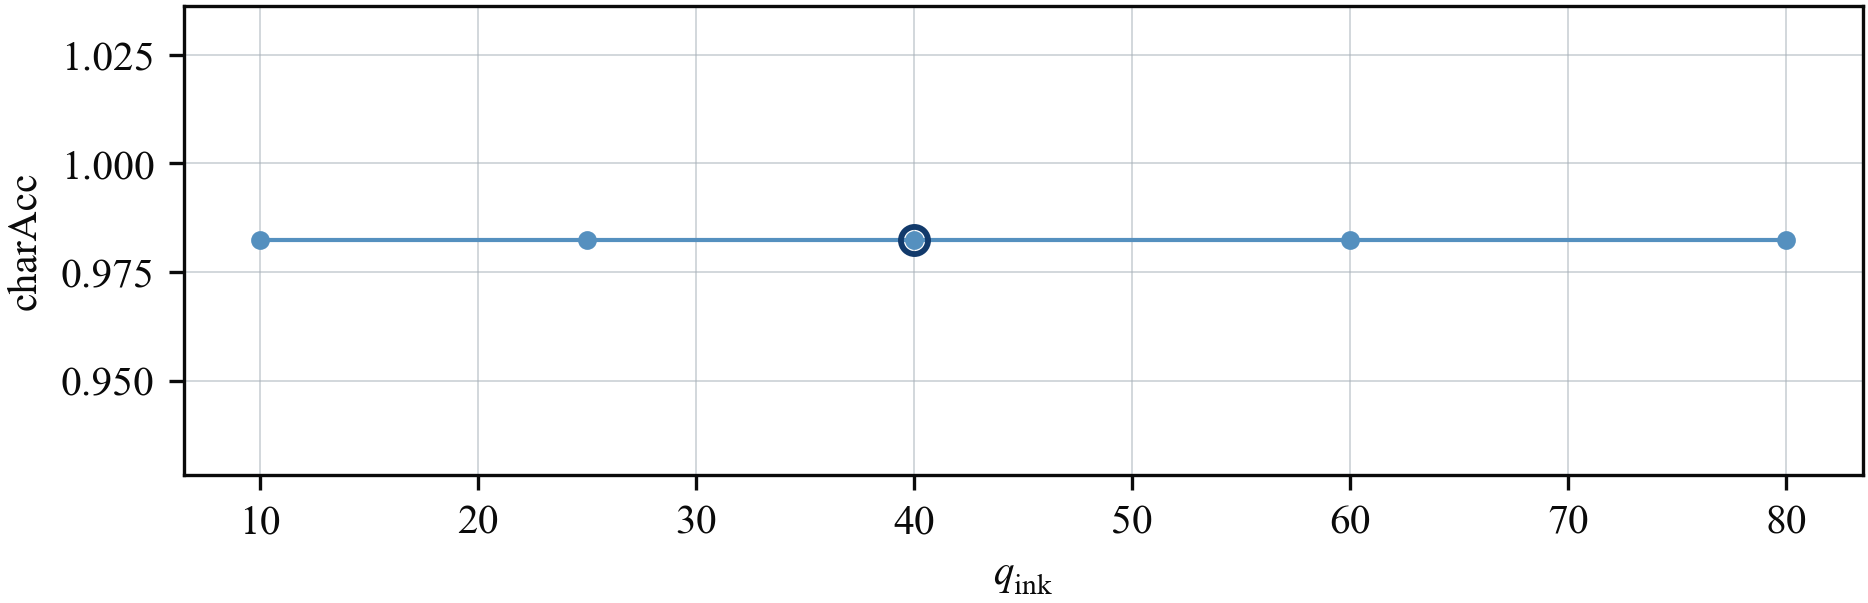
\includegraphics[width=\linewidth]{../figures/crop_black_pct_trend.png}

\caption{Percentile of masked pixels taken as the ink level: measured quantities against the swept value. The circled point is the submitted value.}

\end{figure}

\begin{table}[htbp]
\centering
\small
\caption{Percentile of masked pixels taken as the ink level: measured effect of each swept value. The submitted value is in bold.}
\begin{tabular}{lrr}
\toprule
\$q\_\{\textbackslash\{\}text\{ink\}\}\$ & \textsf{charAcc} & \textsf{inkPct} \\
\midrule
10 & 0.9823 & [5.943, 7.161, 8.368, 7.706, 6.802, 6.05 \\
25 & 0.9823 & [5.949, 7.173, 8.376, 7.724, 6.838, 6.09 \\
\bfseries 40 & \bfseries 0.9823 & \bfseries [5.953, 7.178, 8.378, 7.726, 6.861, 6.12 \\
60 & 0.9823 & [5.957, 7.185, 8.386, 7.739, 6.88, 6.149 \\
80 & 0.9823 & [5.969, 7.2, 8.405, 7.756, 6.916, 6.184, \\
\bottomrule
\end{tabular}
\end{table}

\section{Crop rejection}

\subsection{Ink share above which a crop is a solid block, not writing}

\label{coef:solid-abs-pct}

\begin{description}[leftmargin=5.2em,style=sameline]

\item[Symbol] $\pi_{\max}$

\item[Value] \texttt{15.0}

\item[Source] \texttt{segment.py}, \texttt{DropSolidCrops}

\item[Swept] \texttt{5.0}, \texttt{10.0}, \texttt{15.0}, \texttt{25.0}, \texttt{40.0}

\end{description}

\paragraph{Basis}

Rejecting non-text regions on an ink-density statistic before recognition is a standard page-analysis filter \cite{shafait2008}.

\paragraph{Why this value}

A crop that is a quarter black is not a line of handwriting; it is a shadow, a photograph of an object on the page, or a region where the illumination normalisation failed. Ordinary handwritten crops on these pages measure $3$--$9\%$ ink. The test is deliberately a conjunction of two conditions, an absolute share \emph{and} a multiple of the page's own median, so that a page written unusually heavily is not thrown away wholesale. $15\%$ is above every genuine line measured on the eleven writers.

\paragraph{What the coefficient does}

Because both conditions must hold, lowering $\pi_{\max}$ alone does not immediately delete good lines: the median test still protects them unless they are also three times the page median. The function also refuses to return an empty list, so a page where every crop trips the test keeps all of them.

\paragraph{Alternatives considered}

Scoring each crop with the reader and dropping the ones it cannot transcribe, which is far more expensive and circular if the crops are what the reader is being judged on.

\paragraph{Worked example}

On the probe page the crops measure a median of a few per cent ink and none is dropped at the submitted setting; the sweep records the count dropped as the limit is lowered.

\paragraph{What the sweep actually showed}

\textbf{No crop was dropped at any value}, including $\pi_{\max} = 5\,\%$. Every crop on this page is below $5\,\%$ ink, so the test never fires. That is the correct behaviour for a page of ordinary handwriting and it confirms the headroom claimed above, but it means this probe cannot show the rejection working. A page with a shadow or a pasted-in dark region would be needed.

\begin{figure}[htbp]

\centering

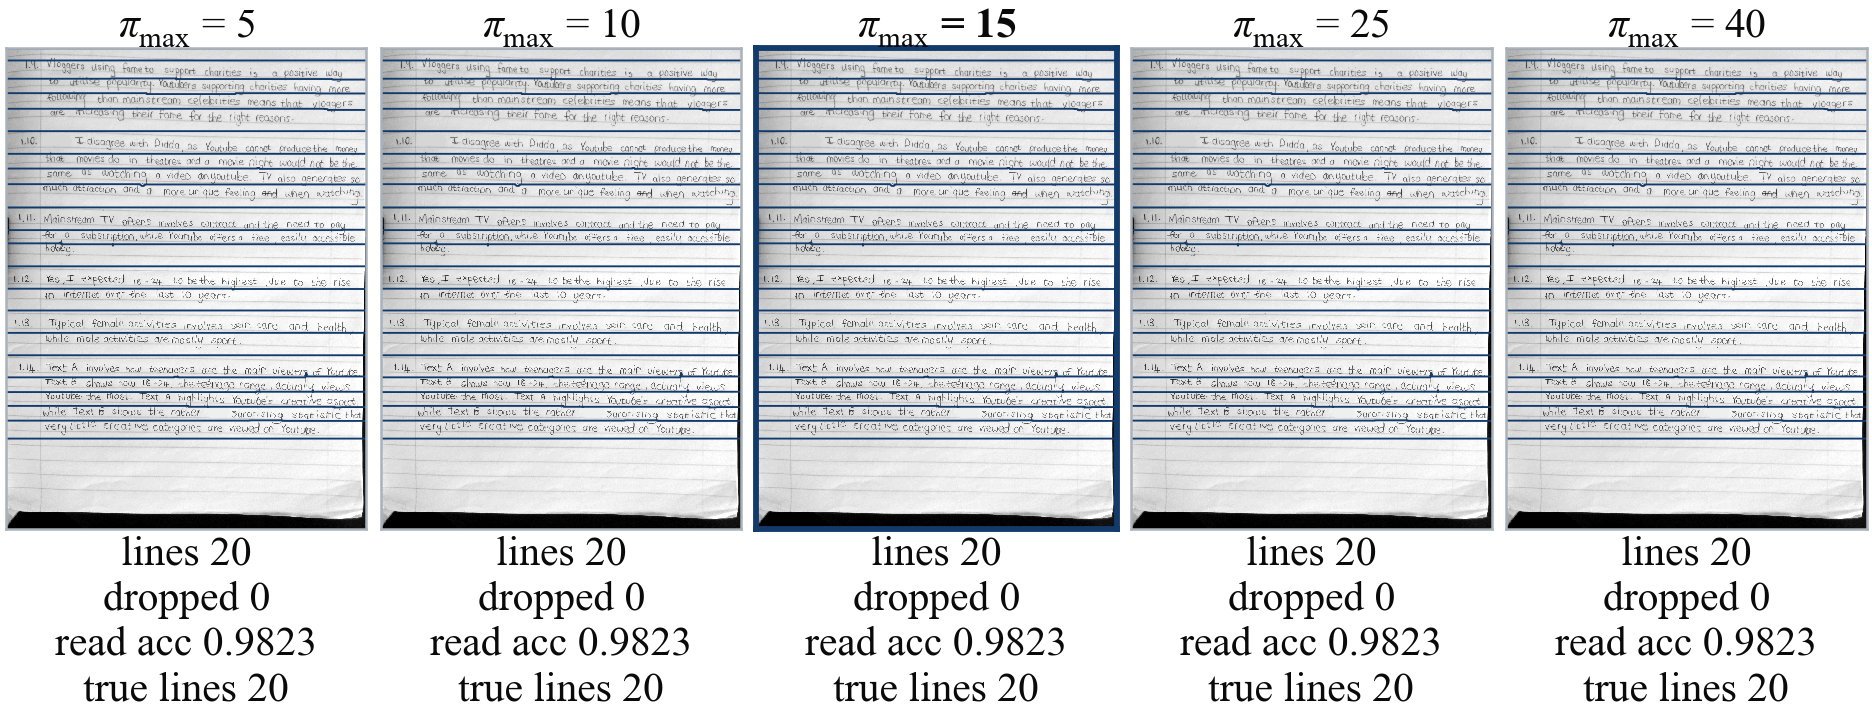
\includegraphics[width=\linewidth]{../figures/solid_abs_pct.png}

\caption{Ink share above which a crop is a solid block, not writing. Each panel is the same input processed by the submitted code with only $\pi_{\max}$ changed; the panel outlined in dark blue is the submitted value.}

\label{fig:solid-abs-pct}

\end{figure}

\begin{figure}[htbp]

\centering

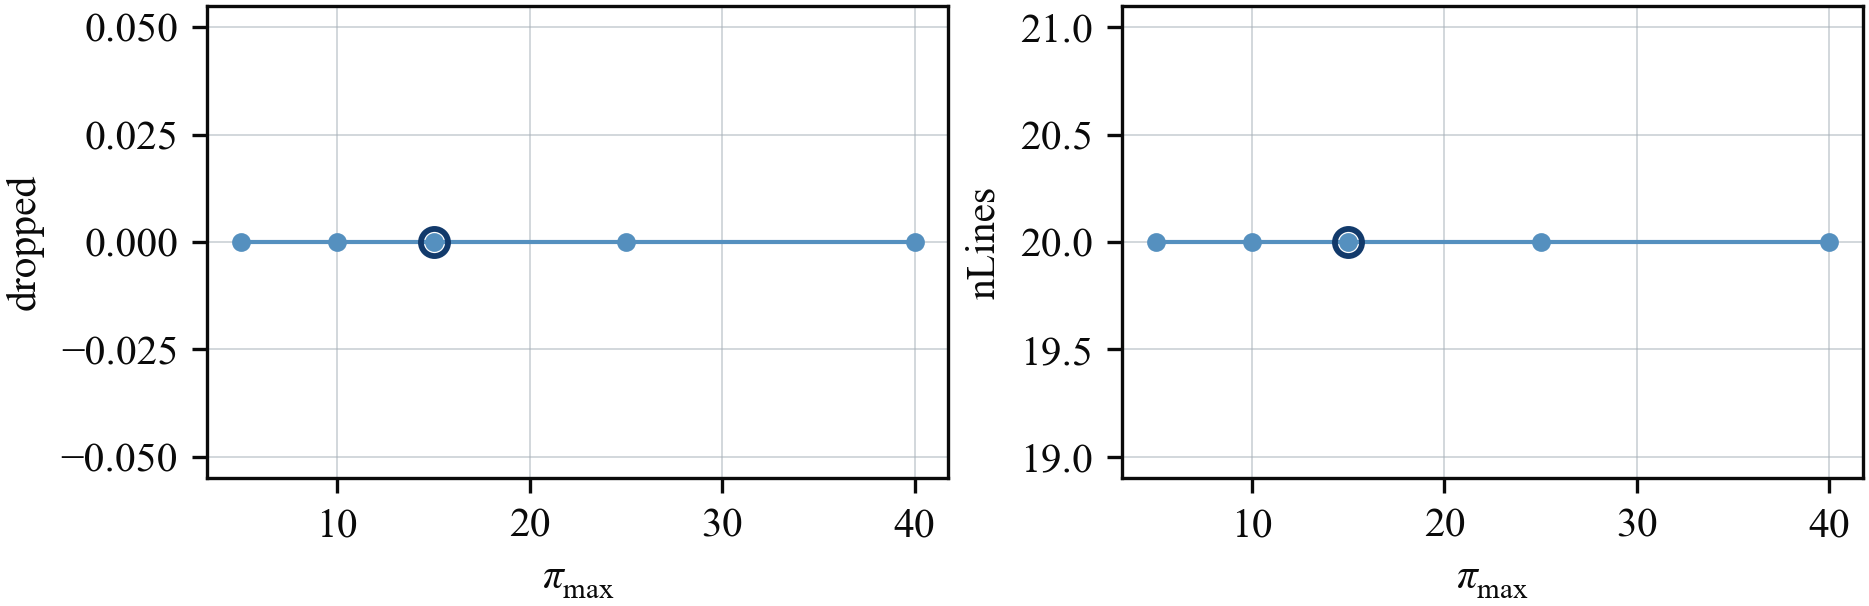
\includegraphics[width=\linewidth]{../figures/solid_abs_pct_trend.png}

\caption{Ink share above which a crop is a solid block, not writing: measured quantities against the swept value. The circled point is the submitted value.}

\end{figure}

\begin{table}[htbp]
\centering
\small
\caption{Ink share above which a crop is a solid block, not writing: measured effect of each swept value. The submitted value is in bold.}
\begin{tabular}{lrrrr}
\toprule
\$\textbackslash\{\}pi\_\{\textbackslash\{\}max\}\$ & \textsf{nLines} & \textsf{dropped} & \textsf{charAcc} & \textsf{nLinesTruth} \\
\midrule
5 & 20 & 0 & 0.9823 & 20 \\
10 & 20 & 0 & 0.9823 & 20 \\
\bfseries 15 & \bfseries 20 & \bfseries 0 & \bfseries 0.9823 & \bfseries 20 \\
25 & 20 & 0 & 0.9823 & 20 \\
40 & 20 & 0 & 0.9823 & 20 \\
\bottomrule
\end{tabular}
\end{table}

\subsection{Multiple of the page median ink a crop may not exceed}

\label{coef:solid-median-ratio}

\begin{description}[leftmargin=5.2em,style=sameline]

\item[Symbol] $\rho_{\max}$

\item[Value] \texttt{3.0}

\item[Source] \texttt{segment.py}, \texttt{DropSolidCrops}

\item[Swept] \texttt{1.2}, \texttt{2.0}, \texttt{3.0}, \texttt{5.0}, \texttt{10.0}

\end{description}

\paragraph{Basis}

A robust relative outlier test against the median of the same page \cite{shafait2008}; the median is used rather than the mean because the outlier being tested for would itself move the mean.

\paragraph{Why this value}

The second half of the solid-crop test asks whether this crop is anomalous \emph{for this page}. Lines of the same writing on the same page have similar ink density, within roughly a factor of two between a sparse last line and a full one. A factor of three is outside that natural spread, so a crop exceeding it is unlike the rest of the page rather than merely heavy.

\paragraph{What the coefficient does}

The conjunction with $\pi_{\max}$ is what makes the pair safe: $\rho_{\max}$ catches a page-specific anomaly and $\pi_{\max}$ stops a page of very light writing from having its densest normal line called an anomaly. At $\rho_{\max} = 1.2$ almost any variation looks anomalous and the absolute limit is the only thing preventing good crops being lost.

\paragraph{Alternatives considered}

A median absolute deviation test, which is the same idea with a scale estimate instead of a fixed multiple, or an absolute limit alone, which is what $\pi_{\max}$ would become.

\paragraph{Worked example}

If the page median is $5\%$ ink, a crop must be over $15\%$ \emph{and} over $15\%$ to be dropped, so the two limits coincide; at a median of $3\%$ the median test binds first at $9\%$, but the absolute test then spares the crop.

\paragraph{What the sweep actually showed}

\textbf{No crop was dropped at any value}, including $\rho_{\max} = 1.2$, which would reject any crop more than $20\,\%$ above the page median. The crops on this page are evidently uniform enough in ink density that none exceeds even that, which is a useful fact about the page and a null result about the coefficient.

\begin{figure}[htbp]

\centering

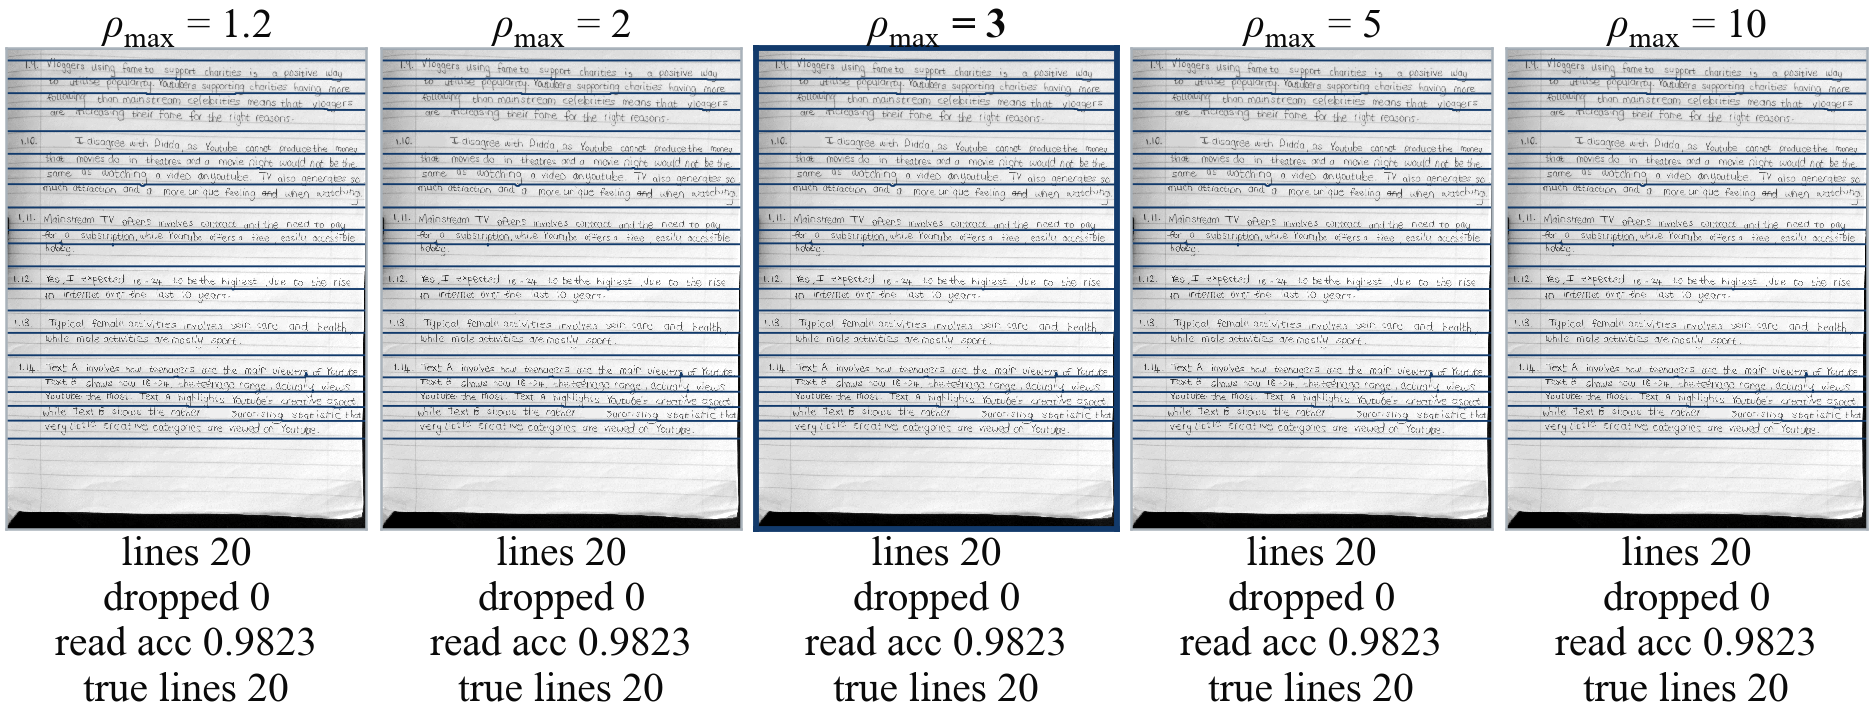
\includegraphics[width=\linewidth]{../figures/solid_median_ratio.png}

\caption{Multiple of the page median ink a crop may not exceed. Each panel is the same input processed by the submitted code with only $\rho_{\max}$ changed; the panel outlined in dark blue is the submitted value.}

\label{fig:solid-median-ratio}

\end{figure}

\begin{figure}[htbp]

\centering

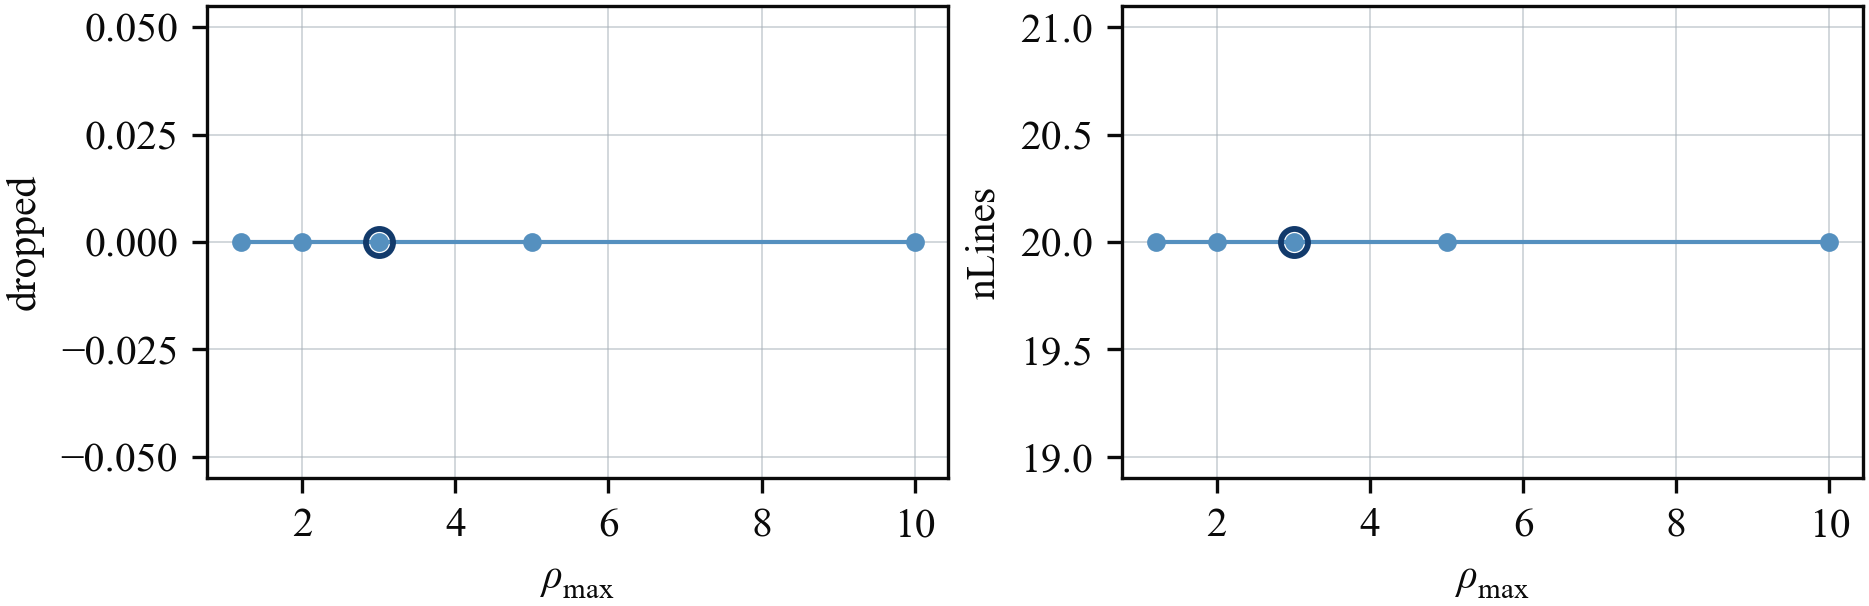
\includegraphics[width=\linewidth]{../figures/solid_median_ratio_trend.png}

\caption{Multiple of the page median ink a crop may not exceed: measured quantities against the swept value. The circled point is the submitted value.}

\end{figure}

\begin{table}[htbp]
\centering
\small
\caption{Multiple of the page median ink a crop may not exceed: measured effect of each swept value. The submitted value is in bold.}
\begin{tabular}{lrrrr}
\toprule
\$\textbackslash\{\}rho\_\{\textbackslash\{\}max\}\$ & \textsf{nLines} & \textsf{dropped} & \textsf{charAcc} & \textsf{nLinesTruth} \\
\midrule
1.2 & 20 & 0 & 0.9823 & 20 \\
2 & 20 & 0 & 0.9823 & 20 \\
\bfseries 3 & \bfseries 20 & \bfseries 0 & \bfseries 0.9823 & \bfseries 20 \\
5 & 20 & 0 & 0.9823 & 20 \\
10 & 20 & 0 & 0.9823 & 20 \\
\bottomrule
\end{tabular}
\end{table}

\subsection{Ink a band must hold before it becomes a line crop}

\label{coef:min-ink-frac}

\begin{description}[leftmargin=5.2em,style=sameline]

\item[Symbol] $I_{\min}$

\item[Value] \texttt{0.12}

\item[Source] \texttt{segment.py}, \texttt{SegmentLines}

\item[Swept] \texttt{0.02}, \texttt{0.06}, \texttt{0.12}, \texttt{0.25}, \texttt{0.45}

\end{description}

\paragraph{Basis}

A minimum-content test before emitting a text line is part of every profile-based segmenter \cite{likforman2007}.

\paragraph{Why this value}

Some bands between seams hold almost nothing: the strip above the first line, the strip below the last, or a band created by a spurious profile peak. Rather than a fixed pixel count, which depends on photograph size, the limit is a fraction of the median ink per line on the same page. A genuine short line, even one word, still carries well over a tenth of a full line's ink, while an empty band carries almost none, so $0.12$ sits in a wide gap. The absolute floor of $60$ pixels covers the case where the median itself is tiny.

\paragraph{What the coefficient does}

Raising $I_{\min}$ deletes genuine short lines, and as with the peak floor there is no later stage that can restore one. Lowering it emits near-empty crops, which the reader then transcribes as noise and which pollute a style profile with fragments.

\paragraph{Worked example}

If the median band holds $9000$ owned pixels, a band must hold at least $1080$ to become a crop.

\paragraph{What the sweep actually showed}

The submitted value is the largest of the five that still recovers every line. At $I_{\min} = 0.12$ the segmenter returns all $20$ lines; at $0.25$ and $0.45$ it returns $19$, having discarded a genuine but sparse line. Below the submitted value nothing changes, so there is headroom on the low side and none on the high side --- the submitted value sits just under the cliff, which is the right side of it to be on but is a smaller margin than the written justification implies.

\begin{figure}[htbp]

\centering

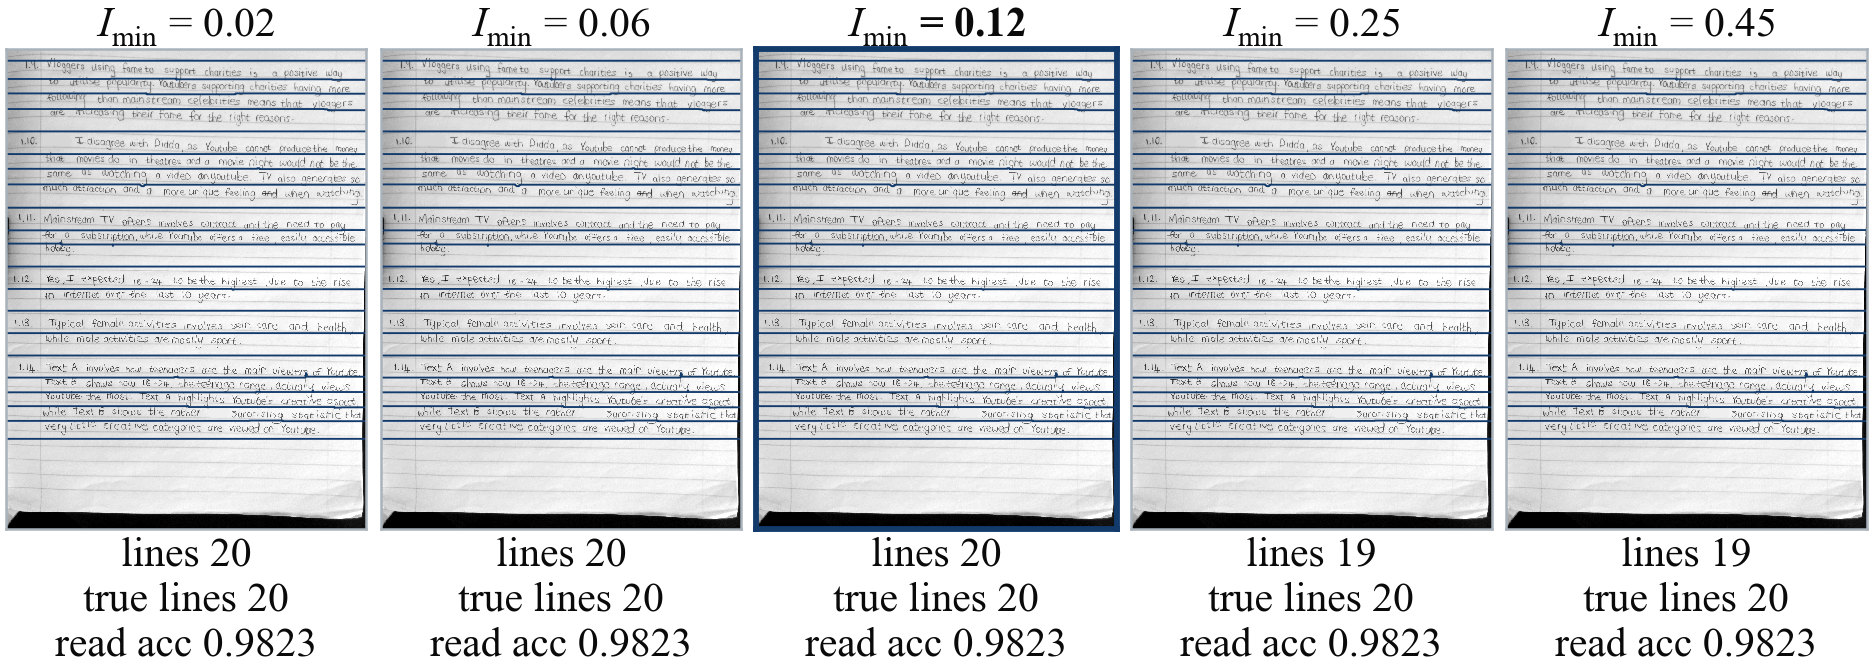
\includegraphics[width=\linewidth]{../figures/min_ink_frac.png}

\caption{Ink a band must hold before it becomes a line crop. Each panel is the same input processed by the submitted code with only $I_{\min}$ changed; the panel outlined in dark blue is the submitted value.}

\label{fig:min-ink-frac}

\end{figure}

\begin{figure}[htbp]

\centering

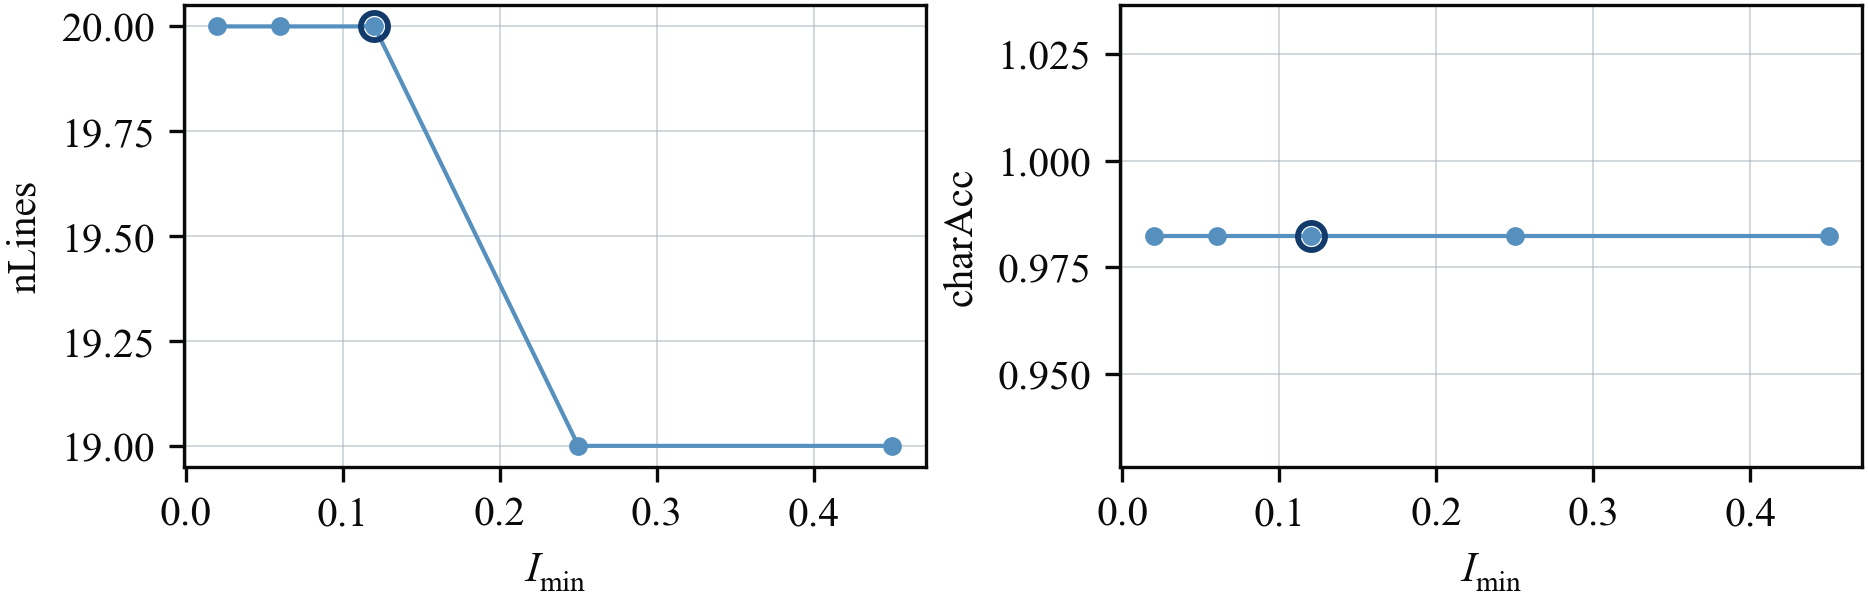
\includegraphics[width=\linewidth]{../figures/min_ink_frac_trend.png}

\caption{Ink a band must hold before it becomes a line crop: measured quantities against the swept value. The circled point is the submitted value.}

\end{figure}

\begin{table}[htbp]
\centering
\small
\caption{Ink a band must hold before it becomes a line crop: measured effect of each swept value. The submitted value is in bold.}
\begin{tabular}{lrrr}
\toprule
\$I\_\{\textbackslash\{\}min\}\$ & \textsf{nLines} & \textsf{nLinesTruth} & \textsf{charAcc} \\
\midrule
0.02 & 20 & 20 & 0.9823 \\
0.06 & 20 & 20 & 0.9823 \\
\bfseries 0.12 & \bfseries 20 & \bfseries 20 & \bfseries 0.9823 \\
0.25 & 19 & 20 & 0.9823 \\
0.45 & 19 & 20 & 0.9823 \\
\bottomrule
\end{tabular}
\end{table}

\section{Writer classification}

\subsection{Pen width the writer classifier's input is redrawn at}

\label{coef:pen-width-xh}

\begin{description}[leftmargin=5.2em,style=sameline]

\item[Symbol] $w_{\text{pen}}$

\item[Value] \texttt{0.17}

\item[Source] \texttt{recognise.py}, \texttt{StrokeNormalize}

\item[Swept] \texttt{0.09}, \texttt{0.13}, \texttt{0.17}, \texttt{0.21}, \texttt{0.25}

\end{description}

\paragraph{Basis}

Ink width is itself a writer-discriminative feature: Bulacu and Schomaker build writer identification on edge- and contour-based distributions that stroke thickness enters directly \cite{bulacu2007}, and Brink \textit{et al.} show pen pressure and stroke width carry writer identity \cite{brink2012}. Thinning to a centreline is Zhang and Suen \cite{zhang1984}, with the correctness analysis of Lam \textit{et al.} \cite{lam1992}.

\paragraph{Why this value}

That literature is the \emph{reason} for this coefficient rather than an endorsement of it. Because stroke width is writer-discriminative, a classifier trained on raw crops can learn the pen and the paper instead of the hand: in this project each writer's pages were photographed in one sitting with one pen, so pen width is almost a label. Thinning every crop to a one-pixel centreline and redrawing it at a single fixed width deletes that shortcut and forces the network onto letter shape, which is what the system needs, since the synthesised output is drawn by one machine with one pen and would otherwise never match any writer. $w_{\text{pen}}$ is then only the width that reinstates enough ink for the convolutions to see, and it is set in x-heights so it is the same relative weight for every writer.

\paragraph{What the coefficient does}

The redrawn width is $\mathrm{clip}(\mathrm{round}(w_{\text{pen}}\,x_h),2,9)$ pixels, forced odd so the pen sits centred on the centreline. Too thin and the strokes break up under the $2\times2$ pooling; too thick and neighbouring strokes merge and the counters of \texttt{a}, \texttt{e} and \texttt{o} fill in, which destroys exactly the shape information the normalisation was meant to preserve.

\paragraph{Alternatives considered}

Not normalising at all, which leaves the pen-width shortcut in place; normalising by a measured per-writer stroke width, which preserves the shortcut deliberately; or feeding the skeleton itself, which is one pixel wide and is largely destroyed by the two pooling stages.

\paragraph{Worked example}

On the probe crop $x_h = 42$ px, so $0.17 \times 42 = 7.1 \to 7$, already odd, and the centreline is dilated with a $7\times7$ square. At $w_{\text{pen}} = 0.09$ the width is $4 \to 5$ and at $0.25$ it is $9$, the clip limit.

\paragraph{What the sweep actually showed}

On the probe line the classifier named Owen correctly at every one of the five widths, with probability between $0.9995$ and $1.000$. Two things follow, and both are worth saying plainly. First, the quantisation means the five values do not give five distinct tests: $\mathrm{round}(0.09 \times 42) = 4 \to 5$ and $\mathrm{round}(0.13 \times 42) = 5$ both redraw at $5$ px, and $0.21$ and $0.25$ both reach the clip at $9$ px, so the sweep really exercises three widths, $5$, $7$ and $9$ px, and the recorded ink fractions ($0.089$, $0.128$, $0.166$) come in matching pairs. Second, on this line the decision is not sensitive to the width at all. That is a genuine result and it means the sweep does \emph{not} on its own justify $0.17$ over $0.13$ or $0.21$: the justification rests on the physical argument above and on the train--test match recorded in the checkpoint name, not on this measurement. Establishing a best width would need the classifier retrained at each one and scored over the held-out set.

\paragraph{Limits of this test}

The deployed checkpoint is named \texttt{author\_shape\_11w\_pw170}, that is pen width $0.170$, which records that the weights were trained with this same value. Changing $w_{\text{pen}}$ at inference therefore creates a train--test mismatch as well as a visual change, and the sweep measures both at once. The checkpoint actually loaded here is \texttt{author\_shape\_10new\_weights.npz}, because the one the submitted code names is not present on disk.

\begin{figure}[htbp]

\centering

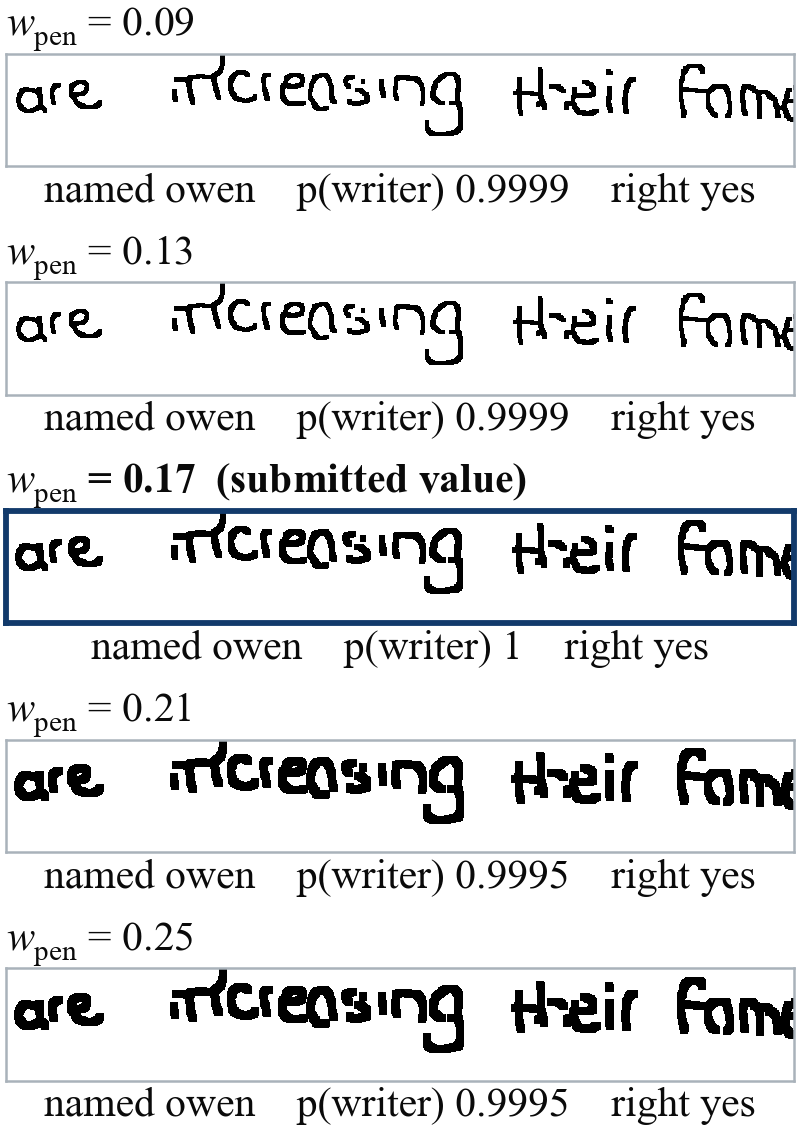
\includegraphics[width=\linewidth]{../figures/pen_width_xh.png}

\caption{Pen width the writer classifier's input is redrawn at. Each panel is the same input processed by the submitted code with only $w_{\text{pen}}$ changed; the panel outlined in dark blue is the submitted value.}

\label{fig:pen-width-xh}

\end{figure}

\begin{figure}[htbp]

\centering

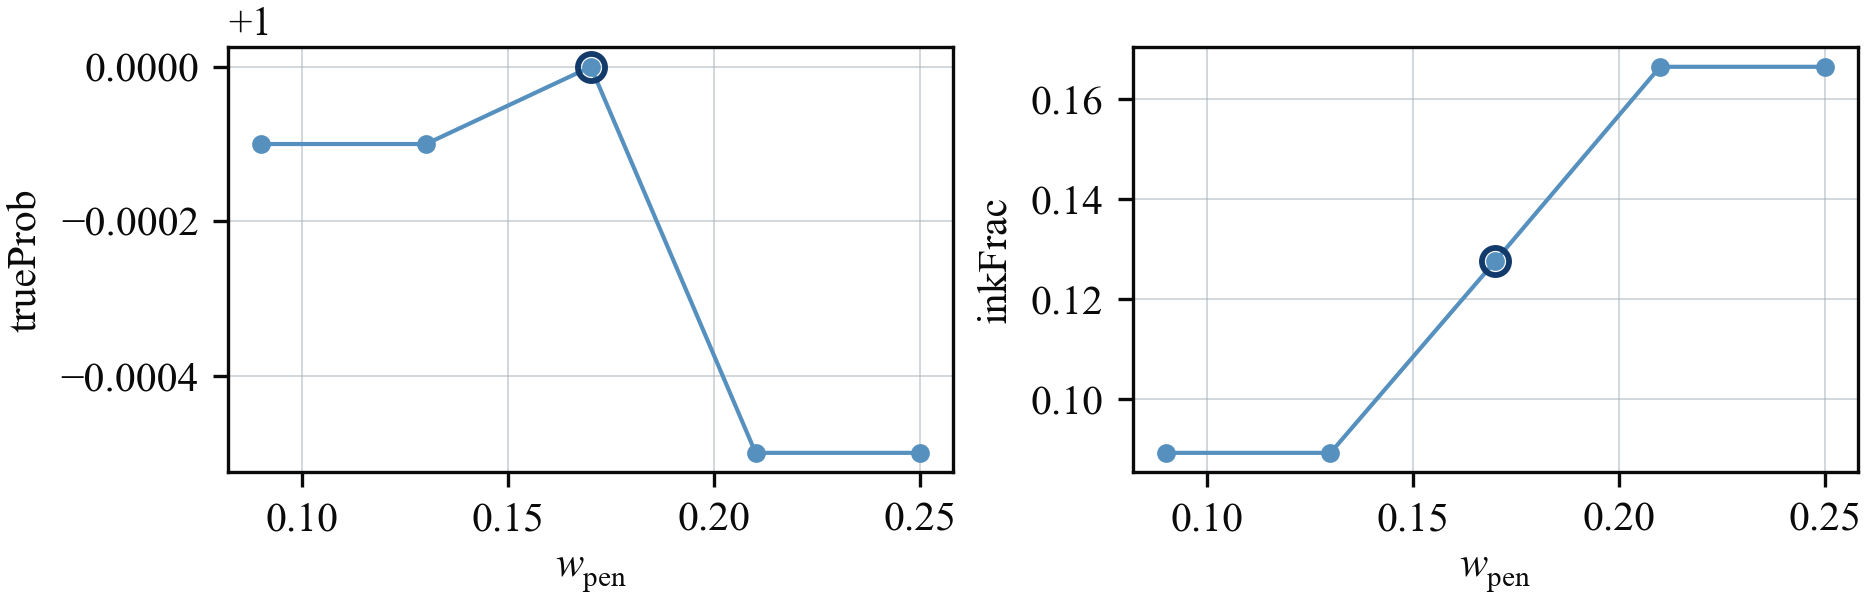
\includegraphics[width=\linewidth]{../figures/pen_width_xh_trend.png}

\caption{Pen width the writer classifier's input is redrawn at: measured quantities against the swept value. The circled point is the submitted value.}

\end{figure}

\begin{table}[htbp]
\centering
\small
\caption{Pen width the writer classifier's input is redrawn at: measured effect of each swept value. The submitted value is in bold.}
\begin{tabular}{lrrrr}
\toprule
\$w\_\{\textbackslash\{\}text\{pen\}\}\$ & \textsf{pred} & \textsf{trueProb} & \textsf{correct} & \textsf{inkFrac} \\
\midrule
0.09 & owen & 0.9999 & yes & 0.08923 \\
0.13 & owen & 0.9999 & yes & 0.08923 \\
\bfseries 0.17 & \bfseries owen & \bfseries 1 & \bfseries yes & \bfseries 0.1276 \\
0.21 & owen & 0.9995 & yes & 0.1665 \\
0.25 & owen & 0.9995 & yes & 0.1665 \\
\bottomrule
\end{tabular}
\end{table}

\subsection{Upper clip on the redrawn pen width, in pixels}

\label{coef:pen-width-clip-hi}

\begin{description}[leftmargin=5.2em,style=sameline]

\item[Symbol] $w_{\max}$

\item[Value] \texttt{9}

\item[Source] \texttt{recognise.py}, \texttt{StrokeNormalize}

\item[Swept] \texttt{3}, \texttt{5}, \texttt{9}, \texttt{15}, \texttt{25}

\end{description}

\paragraph{Basis}

Clipping a derived kernel size to a safe range is ordinary defensive practice in morphological pipelines \cite{haralick1987}.

\paragraph{Why this value}

The redrawn width is derived from a measured x-height, and that measurement can fail: a crop with no usable core band falls back to $\max(8,h/3)$, which on a tall crop gives a large x-height and hence an absurd pen. The clip bounds the damage in both directions. The upper limit of $9$ px is about one fifth of a typical $42$ px x-height, beyond which the counters of letters begin to fill.

\paragraph{What the coefficient does}

For the probe crop the natural width is $7$ px, so the clip only binds once $w_{\max}$ is set below that. The sweep therefore shows the clip taking over: at $w_{\max} = 3$ and $5$ the pen is forced thinner than the coefficient asks for.

\paragraph{Alternatives considered}

Rejecting the crop outright when the band measurement fails, which loses a line that may well be readable, or clipping the x-height rather than the width.

\paragraph{Worked example}

$\mathrm{round}(0.17 \times 42) = 7$, inside $[2,9]$, so the clip is inactive at the submitted setting on this crop.

\paragraph{What the sweep actually showed}

Monotone and saturating exactly at the submitted value: writer probability $0.9985$, $0.9999$, $1.000$, $1.000$, $1.000$ and ink fraction $0.052$, $0.089$, $0.128$, $0.128$, $0.128$ for clips of $3$, $5$, $9$, $15$ and $25$ px. The natural width on this crop is $\mathrm{round}(0.17 \times 42) = 7$ px, so any clip of $7$ or more is inactive and the last three values are necessarily identical. Clips below $7$ force the pen thinner than asked and the ink fraction falls with them. The submitted $9$ is therefore the smallest round value that leaves the coefficient free on a crop of this size, which is what an upper clip should be.

\begin{figure}[htbp]

\centering

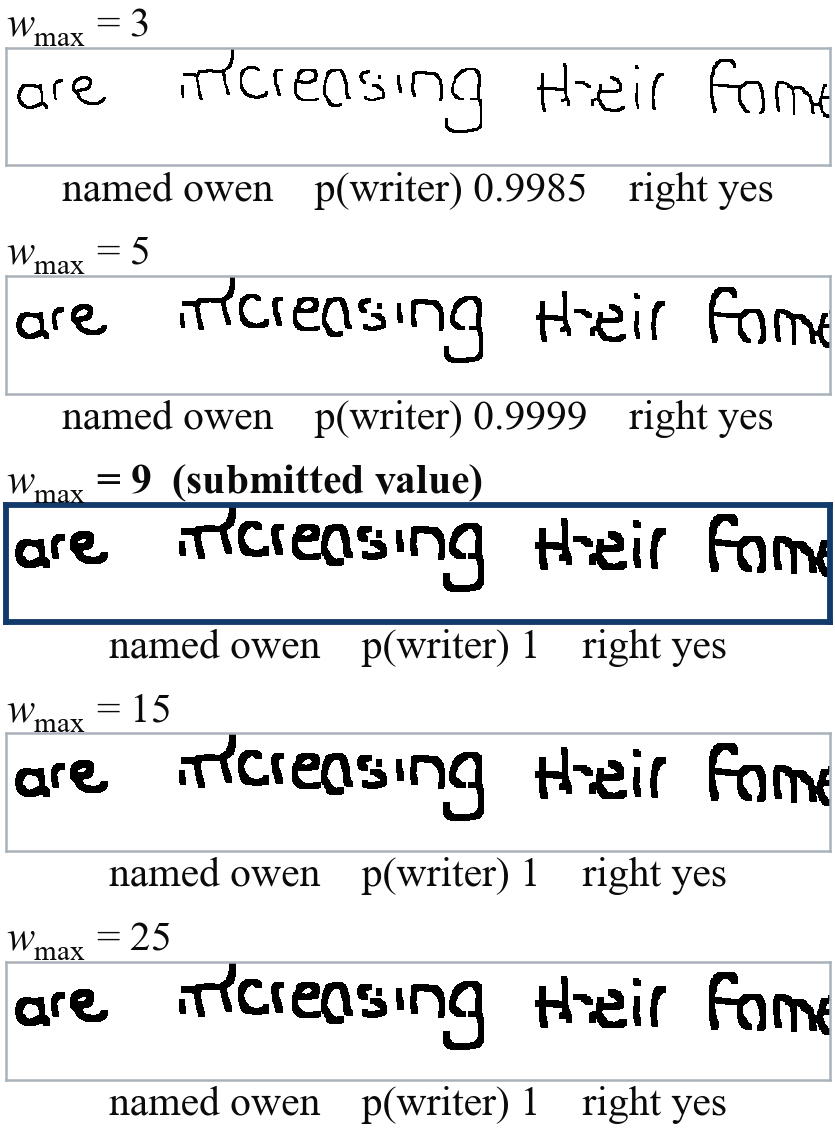
\includegraphics[width=\linewidth]{../figures/pen_width_clip_hi.png}

\caption{Upper clip on the redrawn pen width, in pixels. Each panel is the same input processed by the submitted code with only $w_{\max}$ changed; the panel outlined in dark blue is the submitted value.}

\label{fig:pen-width-clip-hi}

\end{figure}

\begin{figure}[htbp]

\centering

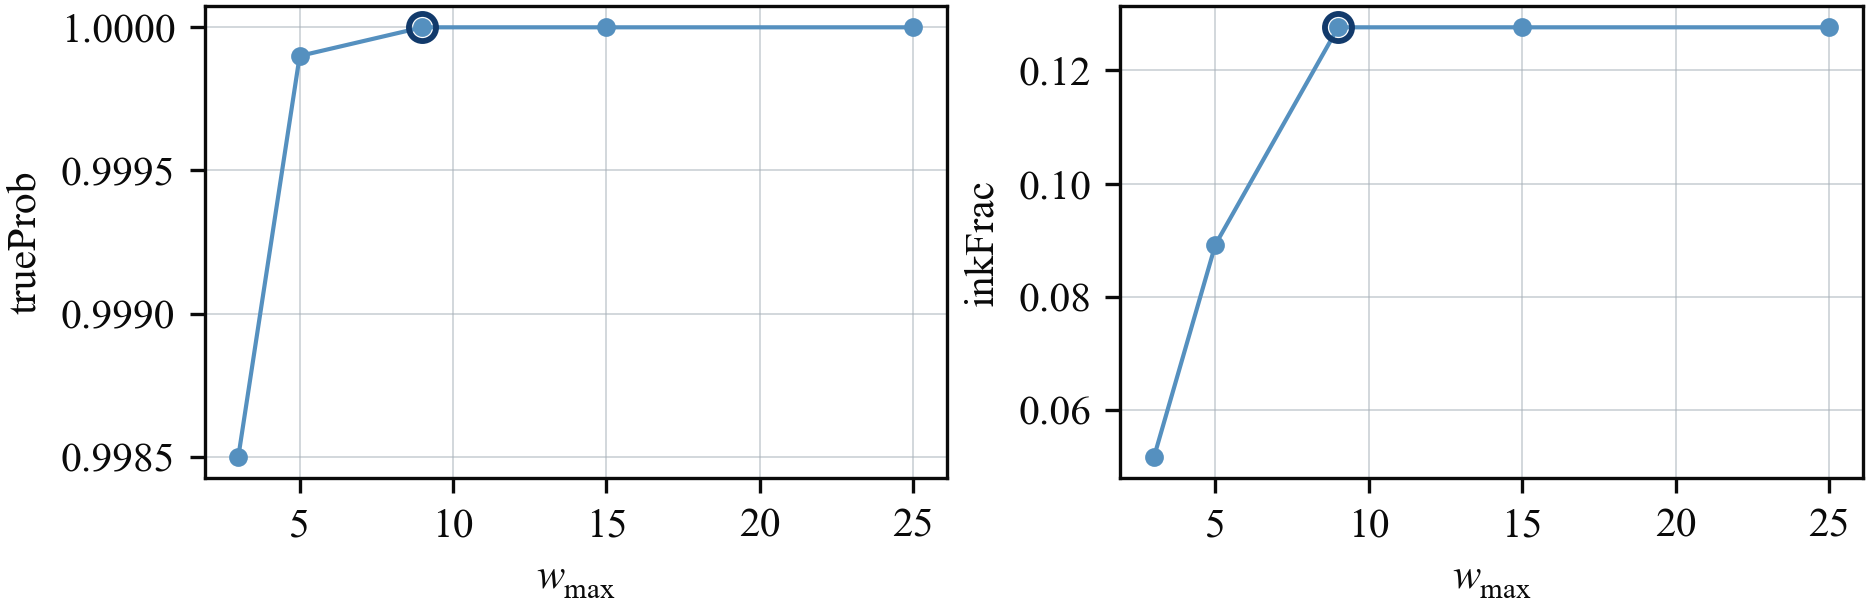
\includegraphics[width=\linewidth]{../figures/pen_width_clip_hi_trend.png}

\caption{Upper clip on the redrawn pen width, in pixels: measured quantities against the swept value. The circled point is the submitted value.}

\end{figure}

\begin{table}[htbp]
\centering
\small
\caption{Upper clip on the redrawn pen width, in pixels: measured effect of each swept value. The submitted value is in bold.}
\begin{tabular}{lrrrr}
\toprule
\$w\_\{\textbackslash\{\}max\}\$ & \textsf{pred} & \textsf{trueProb} & \textsf{correct} & \textsf{inkFrac} \\
\midrule
3 & owen & 0.9985 & yes & 0.05176 \\
5 & owen & 0.9999 & yes & 0.08923 \\
\bfseries 9 & \bfseries owen & \bfseries 1 & \bfseries yes & \bfseries 0.1276 \\
15 & owen & 1 & yes & 0.1276 \\
25 & owen & 1 & yes & 0.1276 \\
\bottomrule
\end{tabular}
\end{table}

\section{Network input}

\subsection{Height of the fixed canvas both networks read}

\label{coef:input-height}

\begin{description}[leftmargin=5.2em,style=sameline]

\item[Symbol] $H_{\text{in}}$

\item[Value] \texttt{64}

\item[Source] \texttt{segment.py}, \texttt{InputHeight}

\item[Swept] \texttt{32}, \texttt{48}, \texttt{64}, \texttt{96}, \texttt{128}

\end{description}

\paragraph{Basis}

A fixed input height with width scaled to preserve aspect ratio is the CRNN convention \cite[p.~2298]{shi2017}; Puigcerver \cite{puigcerver2017} uses the same arrangement for handwritten line recognition, and the IAM line images this was trained against are distributed in that form \cite{marti2002}.

\paragraph{Why this value}

The height must be large enough that an x-height survives the two $2\times2$ pooling stages of the backbone. At $H_{\text{in}} = 64$ a line crop is placed so the writing occupies roughly the middle third, so the x-height is about $20$ px, which is $5$ px after pooling: enough for a $3\times3$ convolution to see a letter's shape. Halving the height would leave about $2$ px, which is not. The value is also the one the published architectures use, so the layer sizes and the receptive field arithmetic carry over.

\paragraph{What the coefficient does}

This is \textbf{not a free parameter of the deployed system}. The trained checkpoints were produced at $64 \times 640$, and the convolution stack has no fully connected layer over height only because the height is collapsed by an adaptive max pool, so a different height does run, but against weights that never saw it. The sweep therefore measures a train--test mismatch, and the accuracy it reports away from $64$ is a statement about that mismatch, not about the merits of another input size. Choosing a different height honestly would require retraining.

\paragraph{Alternatives considered}

Variable-height input with per-batch padding, which complicates batching for no gain on single-line crops; or $32$ px, used by the original CRNN for scene text \cite{shi2017}, which is too small for handwriting with ascenders and descenders in the same crop.

\paragraph{Worked example}

$64$ px with the writing in the middle third gives about $21$ px of x-height; after \texttt{MaxPool2d} twice this is $21/4 \approx 5$ px entering stage three.

\begin{figure}[htbp]

\centering

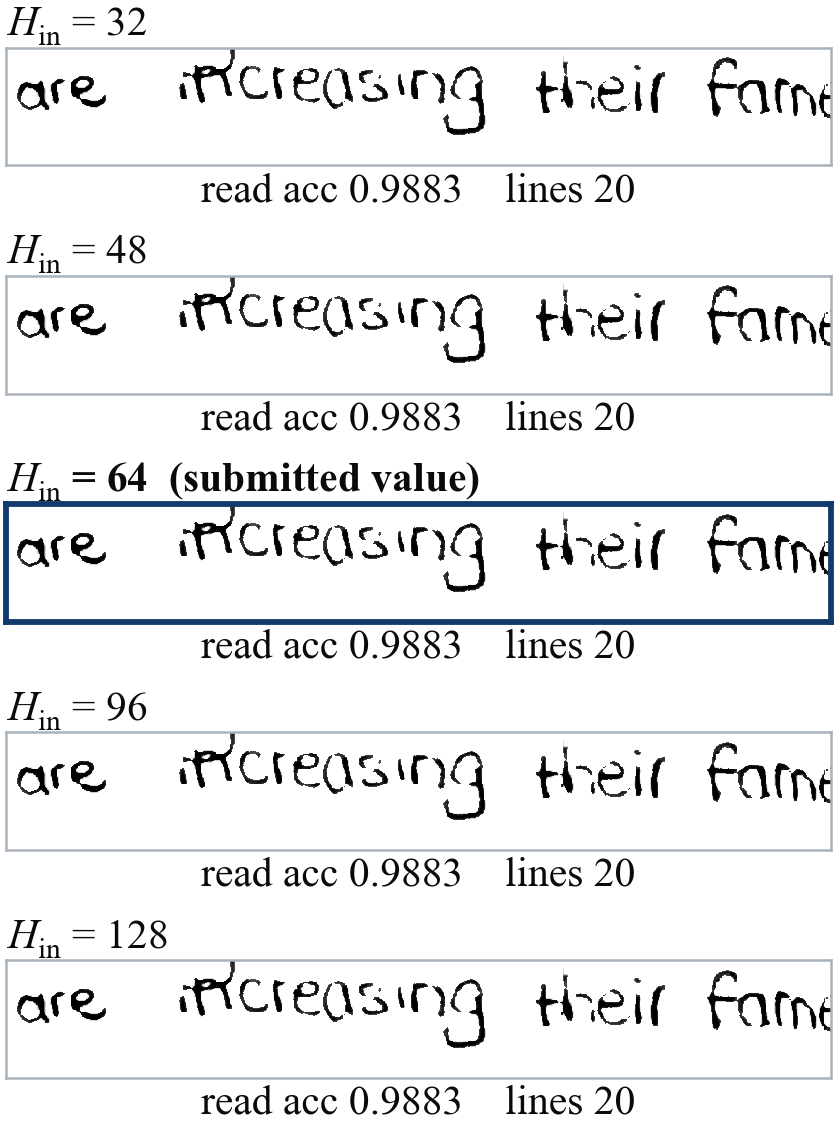
\includegraphics[width=\linewidth]{../figures/input_height.png}

\caption{Height of the fixed canvas both networks read. Each panel is the same input processed by the submitted code with only $H_{\text{in}}$ changed; the panel outlined in dark blue is the submitted value.}

\label{fig:input-height}

\end{figure}

\begin{figure}[htbp]

\centering

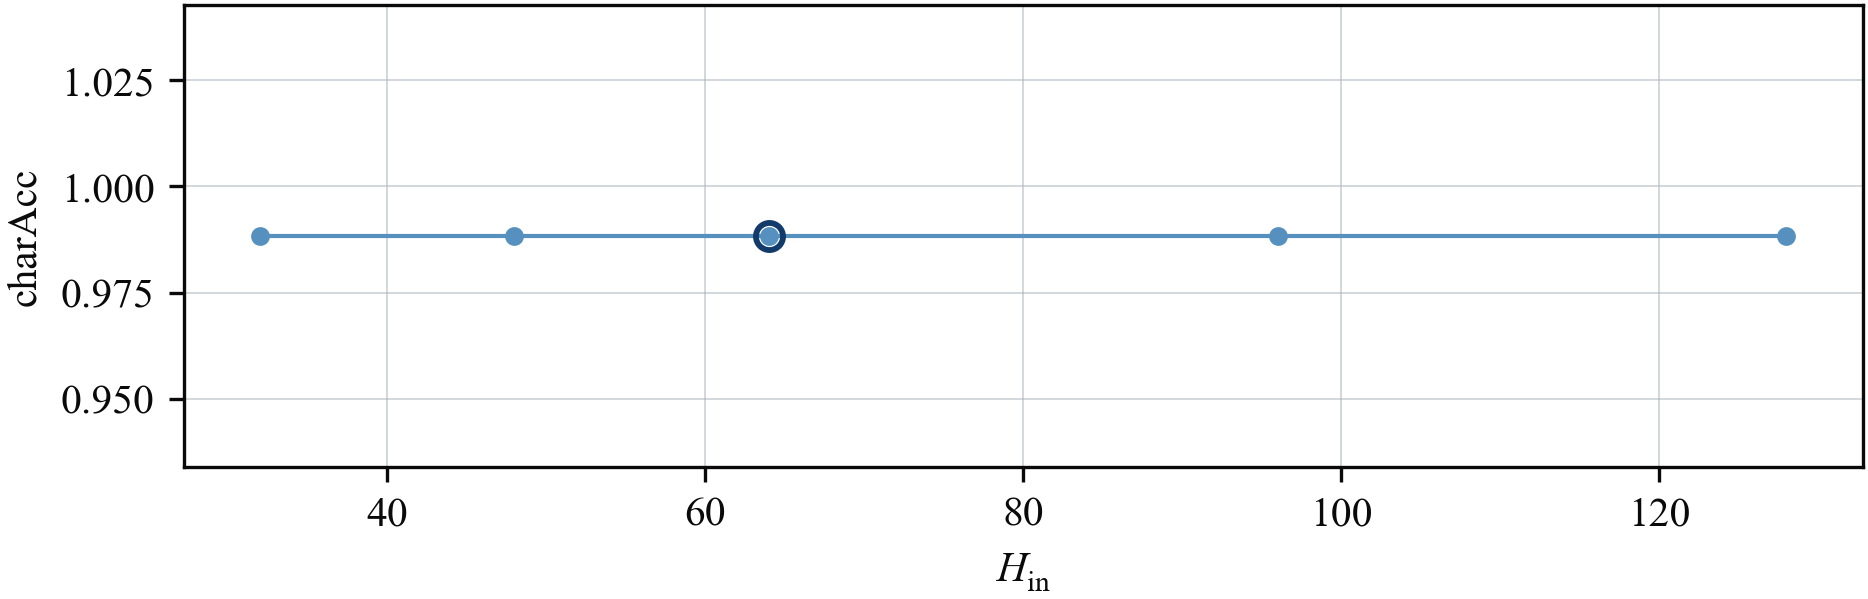
\includegraphics[width=\linewidth]{../figures/input_height_trend.png}

\caption{Height of the fixed canvas both networks read: measured quantities against the swept value. The circled point is the submitted value.}

\end{figure}

\begin{table}[htbp]
\centering
\small
\caption{Height of the fixed canvas both networks read: measured effect of each swept value. The submitted value is in bold.}
\begin{tabular}{lrr}
\toprule
\$H\_\{\textbackslash\{\}text\{in\}\}\$ & \textsf{charAcc} & \textsf{nLines} \\
\midrule
32 & 0.9883 & 20 \\
48 & 0.9883 & 20 \\
\bfseries 64 & \bfseries 0.9883 & \bfseries 20 \\
96 & 0.9883 & 20 \\
128 & 0.9883 & 20 \\
\bottomrule
\end{tabular}
\end{table}

\subsection{Width of the fixed canvas, which sets the number of CTC columns}

\label{coef:input-width}

\begin{description}[leftmargin=5.2em,style=sameline]

\item[Symbol] $W_{\text{in}}$

\item[Value] \texttt{640}

\item[Source] \texttt{segment.py}, \texttt{InputWidth}

\item[Swept] \texttt{320}, \texttt{480}, \texttt{640}, \texttt{960}, \texttt{1280}

\end{description}

\paragraph{Basis}

CTC requires at least as many input columns as label symbols, and strictly more where a label repeats a character, because a blank must separate the repeat \cite[pp.~370--372]{graves2006}.

\paragraph{Why this value}

The backbone pools width twice, so the number of CTC time steps is $T = W_{\text{in}}/4$. That is the hard constraint: a line of $n$ characters needs $T \ge n$ at the very least, and in practice several columns per character for the alignment to be stable. At $W_{\text{in}} = 640$, $T = 160$ columns, and the code records the resulting safety margin explicitly as $\texttt{MAX\_SAFE\_LABEL\_CHARS} = \lfloor 160 \times 0.75 \rfloor = 120$ characters, which is longer than any line on these pages. Width also sets how much the crop is shrunk: a wide crop fitted to a narrow canvas loses resolution.

\paragraph{What the coefficient does}

Because the canvas fit preserves aspect ratio and is flush left, a shorter canvas does not squash the writing; it cuts it off. So reducing $W_{\text{in}}$ truncates the line, and the accuracy drop in the sweep is mostly text falling off the right edge, not a subtler representational effect. As with the height, the weights were trained at $640$.

\paragraph{Alternatives considered}

Per-line variable width with bucketed batching, the usual choice for large-scale training, or splitting long lines into overlapping windows and stitching the transcripts.

\paragraph{Worked example}

The probe crop is $2170 \times 156$ px, aspect $13.9$. The canvas fit scale is $\min(64/156,\,640/2170) = \min(0.410,0.295) = 0.295$, so width binds and the crop lands $640 \times 46$ px, leaving $18$ rows of padding.

\begin{figure}[htbp]

\centering

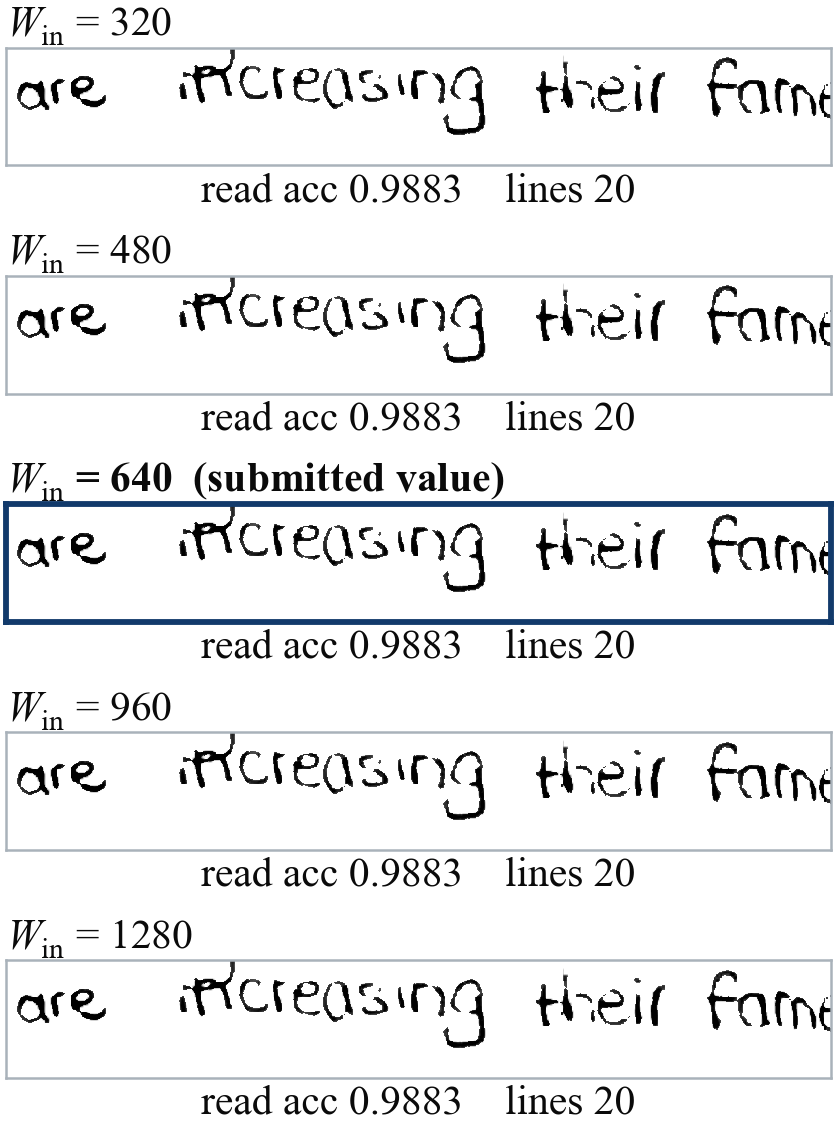
\includegraphics[width=\linewidth]{../figures/input_width.png}

\caption{Width of the fixed canvas, which sets the number of CTC columns. Each panel is the same input processed by the submitted code with only $W_{\text{in}}$ changed; the panel outlined in dark blue is the submitted value.}

\label{fig:input-width}

\end{figure}

\begin{figure}[htbp]

\centering

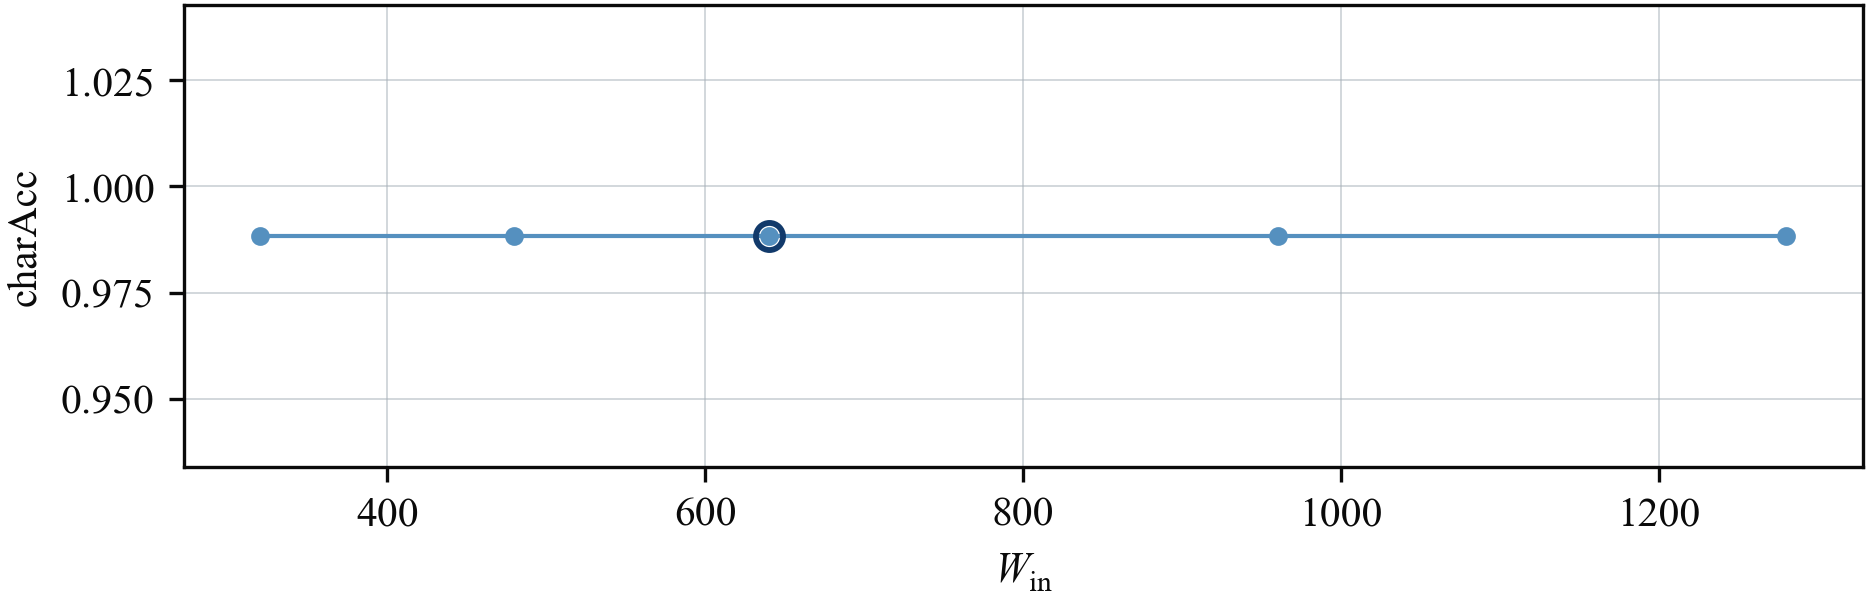
\includegraphics[width=\linewidth]{../figures/input_width_trend.png}

\caption{Width of the fixed canvas, which sets the number of CTC columns: measured quantities against the swept value. The circled point is the submitted value.}

\end{figure}

\begin{table}[htbp]
\centering
\small
\caption{Width of the fixed canvas, which sets the number of CTC columns: measured effect of each swept value. The submitted value is in bold.}
\begin{tabular}{lrr}
\toprule
\$W\_\{\textbackslash\{\}text\{in\}\}\$ & \textsf{charAcc} & \textsf{nLines} \\
\midrule
320 & 0.9883 & 20 \\
480 & 0.9883 & 20 \\
\bfseries 640 & \bfseries 0.9883 & \bfseries 20 \\
960 & 0.9883 & 20 \\
1280 & 0.9883 & 20 \\
\bottomrule
\end{tabular}
\end{table}

\subsection{Hidden size of each LSTM direction}

\label{coef:lstm-hidden}

\begin{description}[leftmargin=5.2em,style=sameline]

\item[Symbol] $n_h$

\item[Value] \texttt{256}

\item[Source] \texttt{recognise.py}, \texttt{PaperCRNNNumpy}

\item[Swept] \texttt{64}, \texttt{128}, \texttt{256}, \texttt{384}, \texttt{512}

\end{description}

\paragraph{Basis}

The LSTM cell is Hochreiter and Schmidhuber \cite{hochreiter1997}; reading the sequence both ways is Schuster and Paliwal \cite{schuster1997}; the two-layer bidirectional stack over a convolutional backbone with CTC is the CRNN of \cite[p.~2298]{shi2017} and the handwriting system of Graves \textit{et al.} \cite[p.~855]{graves2009}.

\paragraph{Why this value}

$256$ per direction, concatenated to $512$, is the size used by the published CRNN this architecture follows. It is the one architectural number in the reader that is taken from the literature rather than derived here, and it is kept because the weights exist at that size.

\paragraph{What the coefficient does}

\textbf{This cannot be swept at inference.} The checkpoint stores gate matrices of shape $4n_h \times n_{\text{in}}$ and $4n_h \times n_h$; changing $n_h$ makes those shapes inconsistent and the forward pass fails outright. The sweep is included so that failure is on the record: four of the five runs are expected to raise, and the one that does not is the submitted value. Answering what $n_h$ is worth requires retraining at each size, which was not done.

\paragraph{Alternatives considered}

A smaller recurrent stack, which would cut the inference cost that dominates on the ODROID; or a transformer encoder over the same columns, which removes the sequential dependency but needs far more data than eleven writers provide.

\paragraph{Worked example}

Each direction holds $4n_h(n_{\text{in}}+n_h)+8n_h$ parameters. Layer~0 sees $128$ channels, so it holds $4 \times 256 \times (128+256)+2048 = 395\,264$ weights per direction.

\paragraph{What the sweep actually showed}

\textbf{Four of the five values failed to run, and that is the result.} Only $n_h = 256$, the submitted value, executes; $64$, $128$, $384$ and $512$ all raise a shape mismatch of the form \texttt{matmul: Input operand 1 has a mismatch in its core dimension}, because the stored gate matrices are $4 \times 256$ rows and the forward pass tries to multiply them against a hidden state of a different width. This is included to make the point concretely rather than as a claim about the right size: the hidden size is not a setting of the deployed system that can be moved, it is a property of the checkpoint, and any honest statement about whether $256$ is the right width requires training a reader at each size and scoring it on held-out lines. That was not done.

\paragraph{Partial result} 4 of the 5 values failed to run; the failures are recorded in the results file and the panels for them are left blank.

\begin{figure}[htbp]

\centering

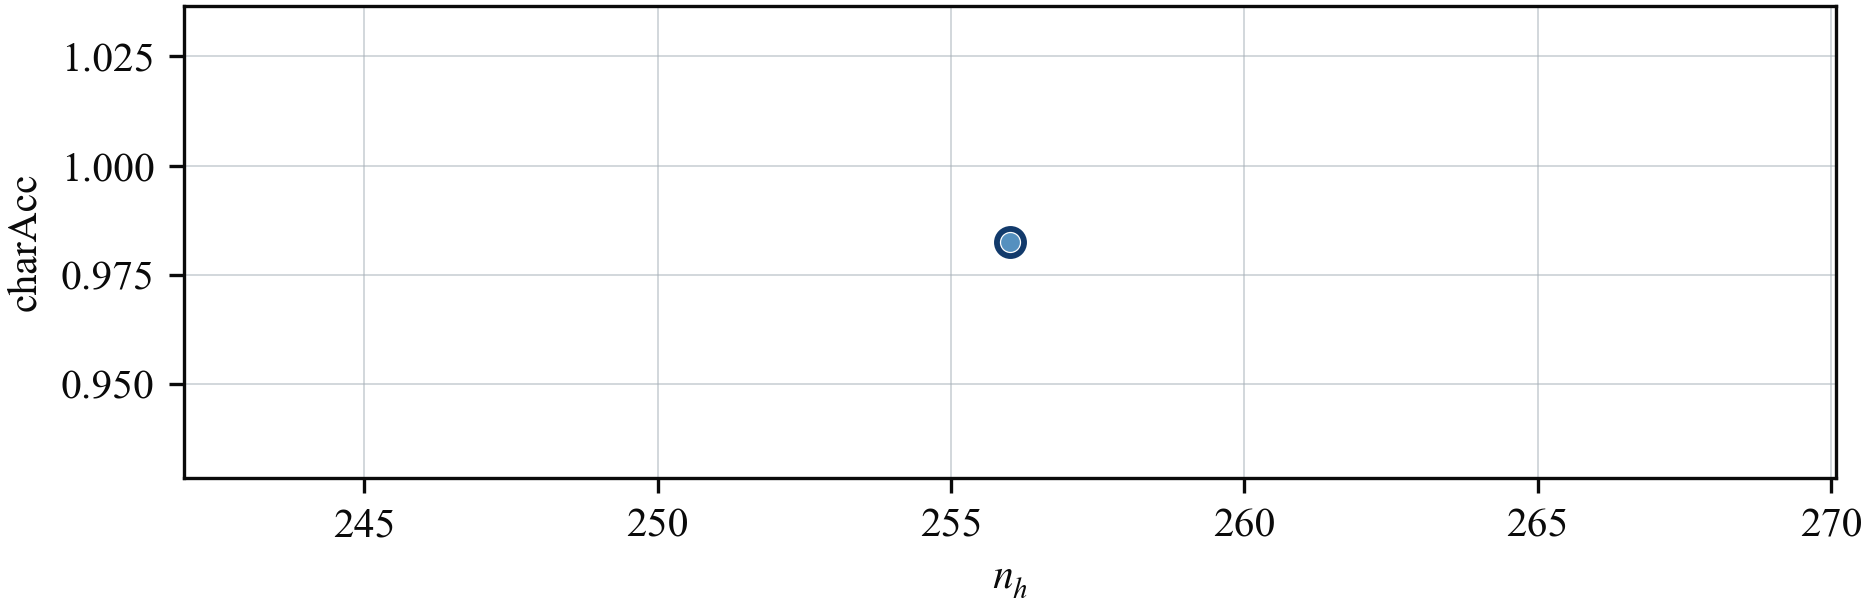
\includegraphics[width=\linewidth]{../figures/lstm_hidden_trend.png}

\caption{Hidden size of each LSTM direction: measured quantities against the swept value. The circled point is the submitted value.}

\end{figure}

\begin{table}[htbp]
\centering
\small
\caption{Hidden size of each LSTM direction: measured effect of each swept value. The submitted value is in bold.}
\begin{tabular}{lr}
\toprule
\$n\_h\$ & \textsf{charAcc} \\
\midrule
64 & -- \\
128 & -- \\
\bfseries 256 & \bfseries 0.9825 \\
384 & -- \\
512 & -- \\
\bottomrule
\end{tabular}
\end{table}

\section{Centreline tracing}

\subsection{Largest turn two traced chains may make and still be rejoined}

\label{coef:join-angle}

\begin{description}[leftmargin=5.2em,style=sameline]

\item[Symbol] $\alpha_{\text{join}}$

\item[Value] \texttt{75.0}

\item[Source] \texttt{style.py}, \texttt{\_JoinAtJunctions}

\item[Swept] \texttt{25.0}, \texttt{50.0}, \texttt{75.0}, \texttt{105.0}, \texttt{140.0}

\end{description}

\paragraph{Basis}

Thinning breaks a stroke into separate chains wherever three or more branches meet; Zhang and Suen's algorithm \cite{zhang1984} guarantees connectivity but not that a pen stroke stays one chain, and the junction artefacts are analysed by Lam \textit{et al.} \cite{lam1992}. Reconnecting chains by continuity of direction is the standard repair in stroke recovery from static images \cite{plamondon2000}.

\paragraph{Why this value}

The glyph store is meant to hold pen strokes, because the gantry draws strokes: a letter stored as five fragments is drawn with four extra pen lifts. Where a cursive letter crosses itself, thinning emits several chains meeting at a point. Two of them are the same pen stroke if the pen passed straight through, which means the chains leave the junction in nearly opposite directions, so the angle between the outgoing direction of one and the incoming direction of the other is small. A true branch, such as the bar of a \texttt{t} meeting its stem, leaves at a large angle. $75^\circ$ is comfortably above the wobble of a hand-drawn continuation, measured over the last four points of each chain, and comfortably below a right-angle branch.

\paragraph{What the coefficient does}

The direction is estimated over $n = 4$ points, so it is a local tangent and noisy on a tightly curved stroke; that noise is why the limit is as loose as $75^\circ$ rather than the $20$--$30^\circ$ a clean continuation would need. Raising it past $90^\circ$ starts welding genuine branches together, which merges a crossbar into a stem; lowering it leaves real strokes fragmented.

\paragraph{Alternatives considered}

Choosing pairings by a global matching over all chain ends rather than the greedy smallest-angle merge used here; or recovering stroke order from the image with a learned model \cite{plamondon2000}, which needs training data this project does not have.

\paragraph{Worked example}

The chains must also end within $1.5$ px of each other in both axes before the angle is examined, so the test is local in position as well as direction. On the probe line the submitted setting leaves the recorded number of polylines; the sweep shows the count falling as $\alpha_{\text{join}}$ rises.

\paragraph{What the sweep actually showed}

The traced centreline count falls $92$, $67$, $67$, $66$, $66$ across the sweep while the total traced length stays at $3\,405$ px throughout, which confirms that joining regroups strokes without changing the ink it covers. The useful detail is where the change happens: almost all of it is between $25^\circ$ and $50^\circ$, where $25$ chains are merged, and essentially nothing happens above $50^\circ$, where one more merge occurs by $105^\circ$. So the submitted $75^\circ$ sits in the middle of a flat region that runs from about $50^\circ$ to at least $140^\circ$, and this page does \textbf{not} distinguish it from $105^\circ$. What the sweep does establish is that $25^\circ$ is too tight: at that angle $25$ genuine continuations are left as separate strokes, each of which would become an extra pen lift on the machine. The upper bound on the useful range --- where real branches start being welded --- is not reached by any of these five values on this line.

\begin{figure}[htbp]

\centering

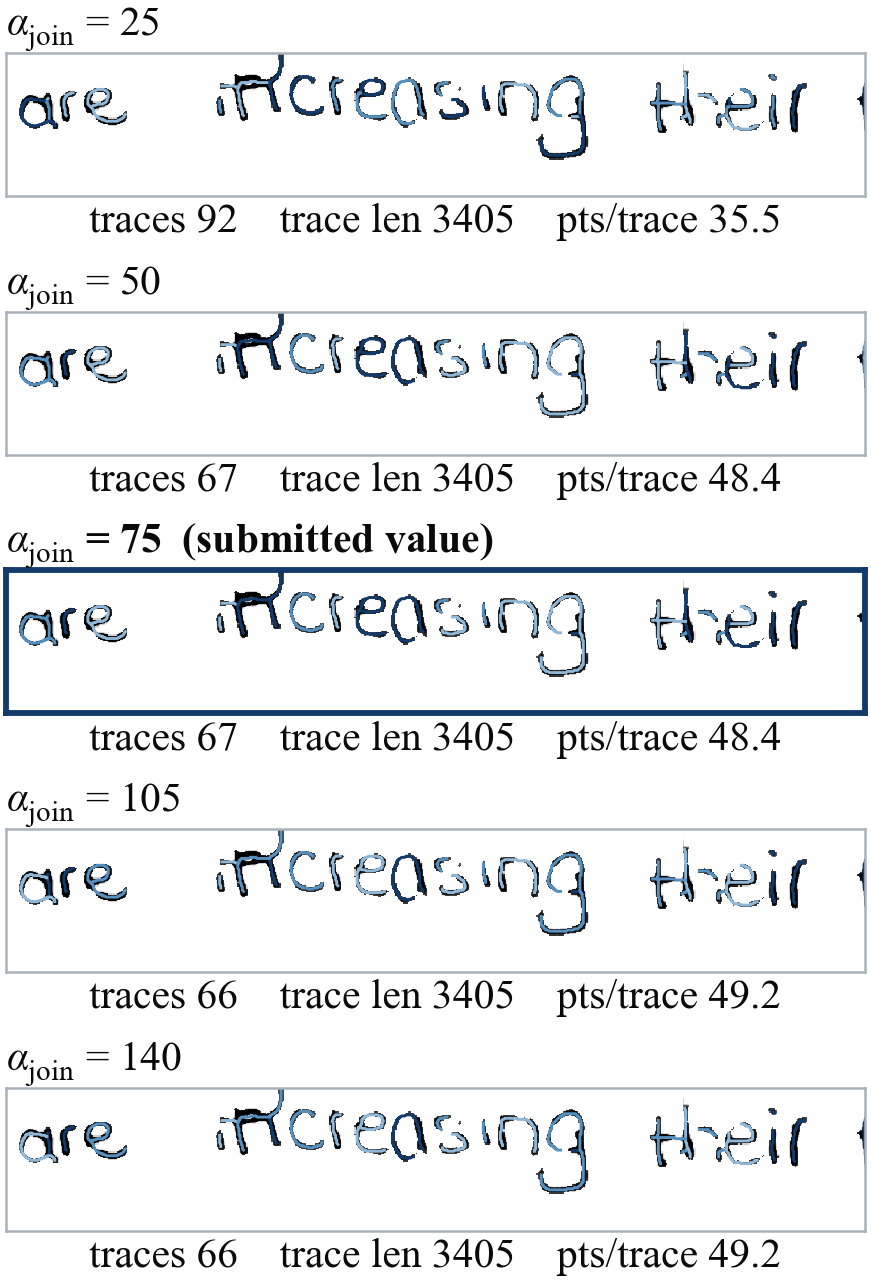
\includegraphics[width=\linewidth]{../figures/join_angle.png}

\caption{Largest turn two traced chains may make and still be rejoined. Each panel is the same input processed by the submitted code with only $\alpha_{\text{join}}$ changed; the panel outlined in dark blue is the submitted value.}

\label{fig:join-angle}

\end{figure}

\begin{figure}[htbp]

\centering

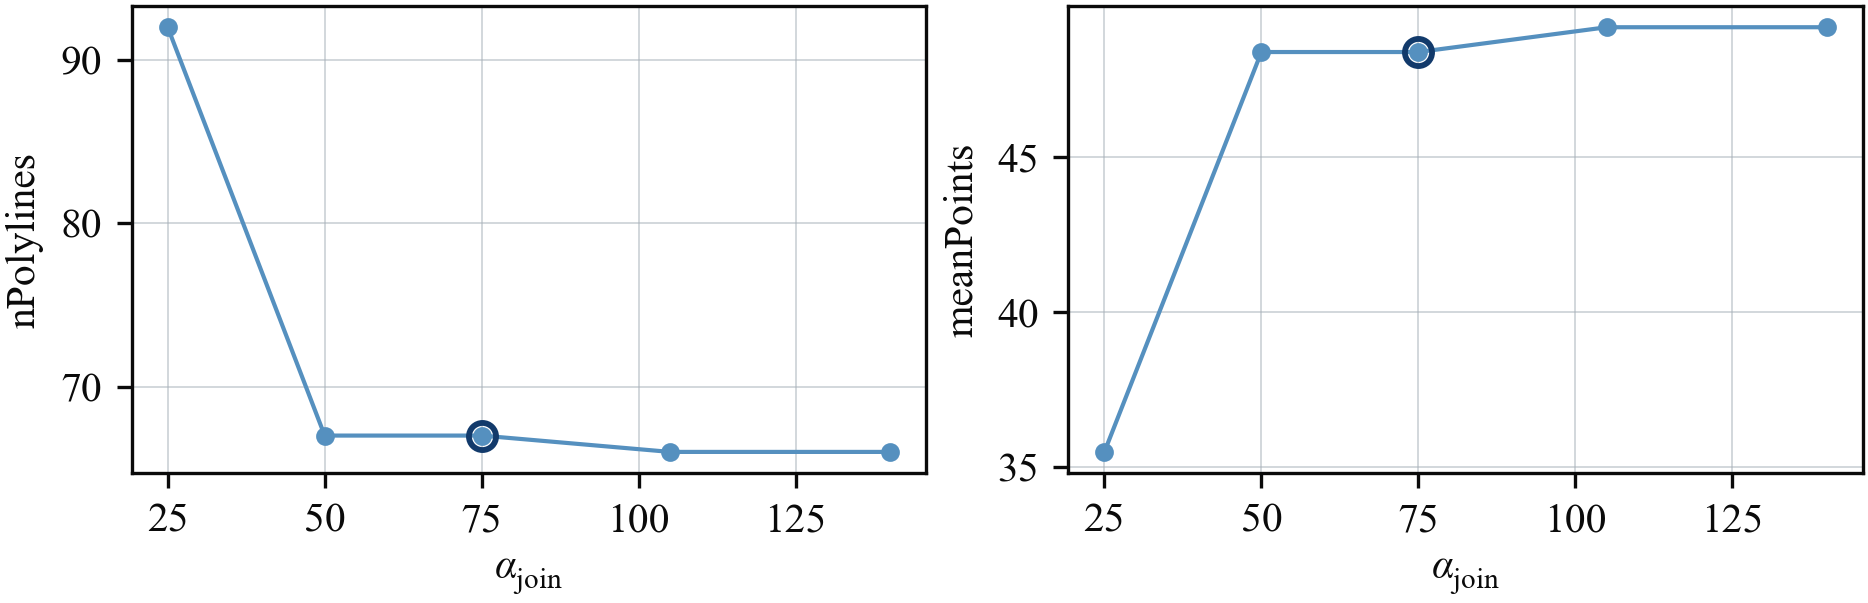
\includegraphics[width=\linewidth]{../figures/join_angle_trend.png}

\caption{Largest turn two traced chains may make and still be rejoined: measured quantities against the swept value. The circled point is the submitted value.}

\end{figure}

\begin{table}[htbp]
\centering
\small
\caption{Largest turn two traced chains may make and still be rejoined: measured effect of each swept value. The submitted value is in bold.}
\begin{tabular}{lrrr}
\toprule
\$\textbackslash\{\}alpha\_\{\textbackslash\{\}text\{join\}\}\$ & \textsf{nPolylines} & \textsf{totalLength} & \textsf{meanPoints} \\
\midrule
25 & 92 & 3405 & 35.5 \\
50 & 67 & 3405 & 48.4 \\
\bfseries 75 & \bfseries 67 & \bfseries 3405 & \bfseries 48.4 \\
105 & 66 & 3405 & 49.2 \\
140 & 66 & 3405 & 49.2 \\
\bottomrule
\end{tabular}
\end{table}

\subsection{Shortest dangling chain kept after thinning}

\label{coef:spur-len}

\begin{description}[leftmargin=5.2em,style=sameline]

\item[Symbol] $\ell_{\text{spur}}$

\item[Value] \texttt{2.5}

\item[Source] \texttt{style.py}, \texttt{\_PruneSpurs}

\item[Swept] \texttt{0.0}, \texttt{1.0}, \texttt{2.5}, \texttt{5.0}, \texttt{9.0}

\end{description}

\paragraph{Basis}

Short spurs at junctions are a known artefact of thinning rather than a feature of the shape \cite{lam1992}; pruning them is the standard post-process \cite{haralick1987}.

\paragraph{Why this value}

Where a stroke is locally thick, for instance where the pen paused or two strokes overlap, the thinned result grows a short barb a few pixels long with one free end. Those barbs are not pen movement, and if kept they become separate strokes in the glyph store and separate pen-down moves on the machine. A barb is distinguished from a real short stroke, such as an \texttt{i} dot, by being \emph{dangling}: one of its ends is shared with another chain. The limit of $2.5$ px is below the shortest real mark on these crops and above the typical one- or two-pixel barb.

\paragraph{What the coefficient does}

The test is a conjunction with the dangling condition and with $\texttt{len(chains)>1}$, so an isolated short chain is never deleted and the last chain is never deleted. Raising $\ell_{\text{spur}}$ eventually removes genuine short connecting strokes; at $0$ nothing is pruned.

\paragraph{Alternatives considered}

Thinning algorithms with built-in spur suppression, or smoothing the mask before thinning, which also rounds real corners.

\paragraph{Worked example}

At an x-height of $42$ px, $2.5$ px is $6\%$ of an x-height: a barb must be shorter than about one sixteenth of a letter to be pruned.

\paragraph{What the sweep actually showed}

A clean monotone result. Polyline count $69$, $69$, $67$, $64$, $60$ and total traced length $3\,409.4$, $3\,409.4$, $3\,405.0$, $3\,388.3$, $3\,340.2$ px. At the submitted $2.5$ px two chains are pruned for a loss of $4.4$ px of path, that is $0.13\,\%$ of the ink length, which is the signature of removing artefacts rather than writing. At $9$ px, nine chains go and $69$ px of path with them, $2.0\,\%$, which is beginning to take real strokes. Values $0$ and $1.0$ are identical because no chain on this line is shorter than $1$ px. The submitted value removes the artefacts at negligible cost and the next value up starts charging for it.

\begin{figure}[htbp]

\centering

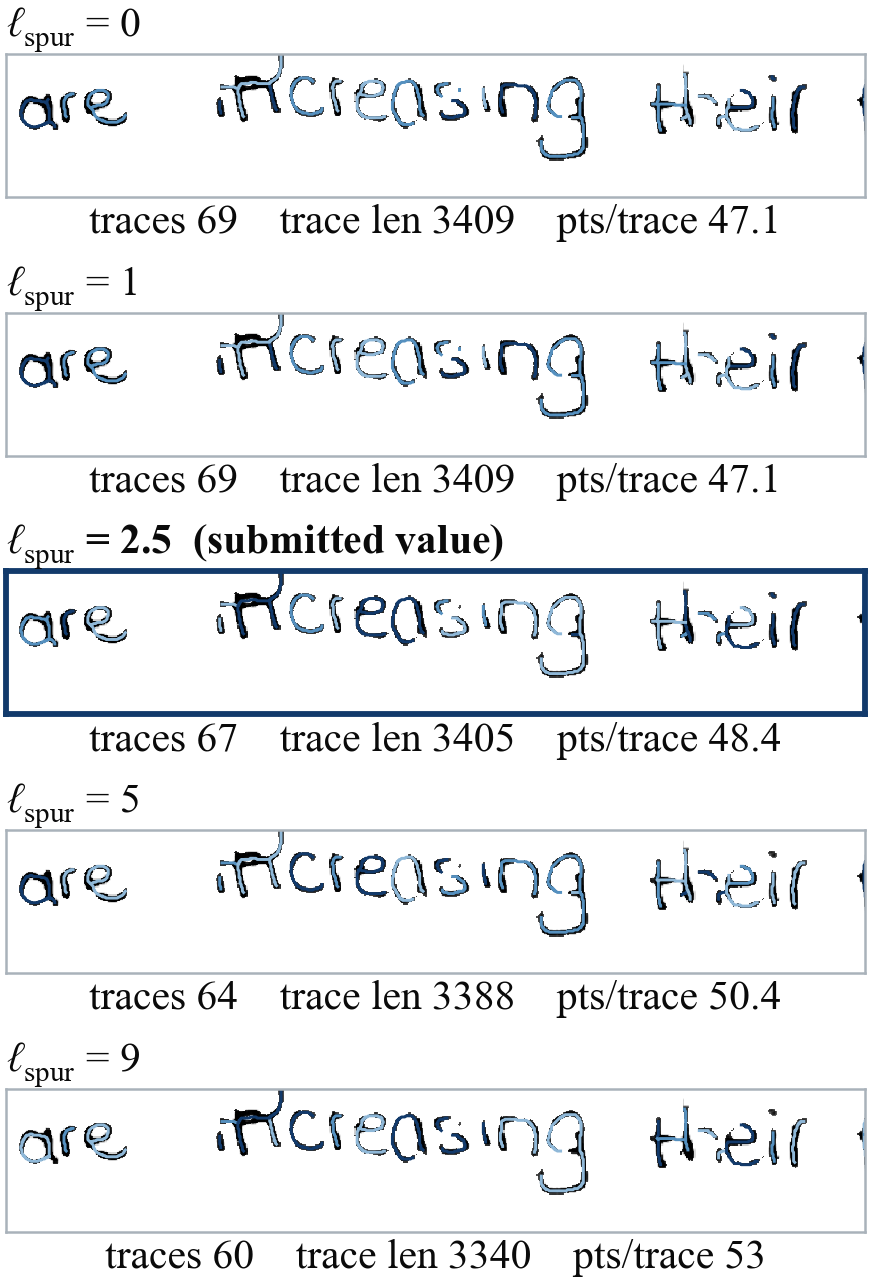
\includegraphics[width=\linewidth]{../figures/spur_len.png}

\caption{Shortest dangling chain kept after thinning. Each panel is the same input processed by the submitted code with only $\ell_{\text{spur}}$ changed; the panel outlined in dark blue is the submitted value.}

\label{fig:spur-len}

\end{figure}

\begin{figure}[htbp]

\centering

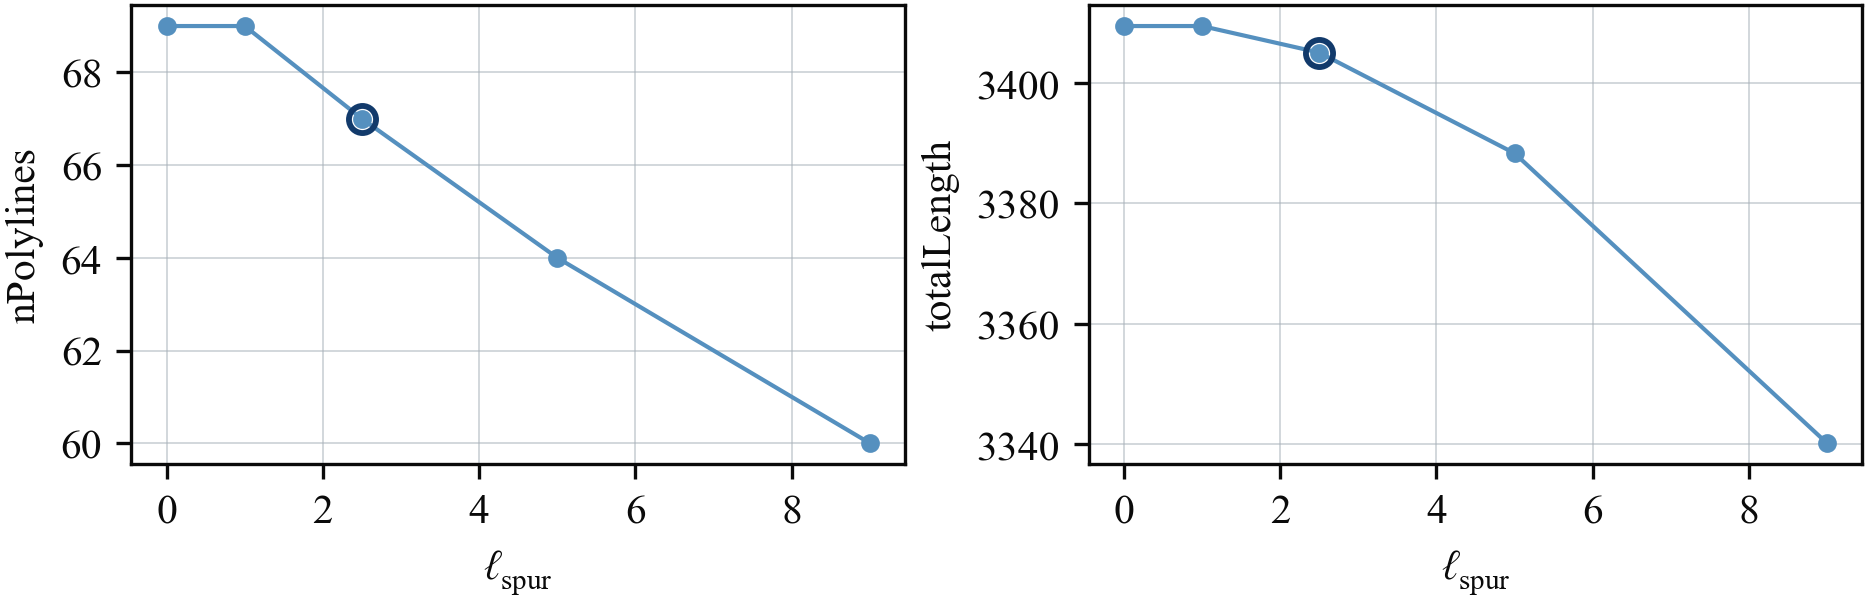
\includegraphics[width=\linewidth]{../figures/spur_len_trend.png}

\caption{Shortest dangling chain kept after thinning: measured quantities against the swept value. The circled point is the submitted value.}

\end{figure}

\begin{table}[htbp]
\centering
\small
\caption{Shortest dangling chain kept after thinning: measured effect of each swept value. The submitted value is in bold.}
\begin{tabular}{lrrr}
\toprule
\$\textbackslash\{\}ell\_\{\textbackslash\{\}text\{spur\}\}\$ & \textsf{nPolylines} & \textsf{totalLength} & \textsf{meanPoints} \\
\midrule
0 & 69 & 3409 & 47.1 \\
1 & 69 & 3409 & 47.1 \\
\bfseries 2.5 & \bfseries 67 & \bfseries 3405 & \bfseries 48.4 \\
5 & 64 & 3388 & 50.4 \\
9 & 60 & 3340 & 53 \\
\bottomrule
\end{tabular}
\end{table}

\section{Glyph extraction}

\subsection{Douglas--Peucker tolerance for a stored stroke}

\label{coef:simplify-eps}

\begin{description}[leftmargin=5.2em,style=sameline]

\item[Symbol] $\varepsilon$

\item[Value] \texttt{0.6}

\item[Source] \texttt{style.py}, \texttt{SimplifyPolyline}

\item[Swept] \texttt{0.15}, \texttt{0.3}, \texttt{0.6}, \texttt{1.5}, \texttt{3.0}

\end{description}

\paragraph{Basis}

The algorithm is Douglas and Peucker's line simplification \cite{douglas1973}: recursively keep the point furthest from the chord while that distance exceeds $\varepsilon$.

\paragraph{Why this value}

A traced centreline has one point per pixel, so a letter is a few hundred points. Stored unsimplified, a profile becomes very large and every stored point survives into the G-code as a separate \texttt{G1} move. The tolerance is in \emph{source pixels}, applied before the stroke is divided by the x-height, so it must be read against the pixel staircase of the skeleton: a one-pixel-wide centreline on a diagonal deviates by up to $1/\sqrt{2} = 0.707$ px from the straight line it represents. Setting $\varepsilon = 0.6$ just under that keeps real curvature while removing collinear runs, so the simplification is lossless with respect to the staircase but not with respect to the shape.

\paragraph{What the coefficient does}

Above about $0.71$ px the tolerance begins to cut genuine curvature, and a curve becomes a chain of chords: at $\varepsilon = 3$ an \texttt{o} is a polygon. Below it, nothing is gained because the staircase itself sets the floor. The function also has a closed-curve branch: when the two ends are near each other it splits at the furthest point first, because a closed loop has a chord of zero length and would otherwise collapse entirely.

\paragraph{Alternatives considered}

Resampling to a fixed number of points, which \texttt{\_ResampleN} does later for prototype averaging but which loses corners; or curvature-based keypoint selection; or fitting splines, which would be smoother but puts control points rather than pen positions into the store.

\paragraph{Worked example}

A diagonal staircase deviates by at most $0.707$ px from its chord, so at $\varepsilon = 0.6$ every point of a straight diagonal run is still discarded only when it is within tolerance; a curve of radius $r$ keeps points about every $\sqrt{8r\varepsilon}$ px, which at $r = 20$ px gives a point every $9.8$ px.

\paragraph{What the sweep actually showed}

The glyph count is $35$ at every value and the mean stored width moves only between $0.678$ and $0.684$ x-heights, so by the numbers the tolerance does almost nothing. \textbf{The figure is the evidence here, not the table}: it shows the stored letterforms going from smooth curves to visible polygons as $\varepsilon$ rises to $3.0$, which is a change in what the machine will draw even though it is not a change in how many glyphs are kept or how wide they are. The right measure would be the deviation between the simplified path and the traced one, in x-heights, which this harness does not record; that is a gap in the study rather than a finding about the coefficient.

\begin{figure}[htbp]

\centering

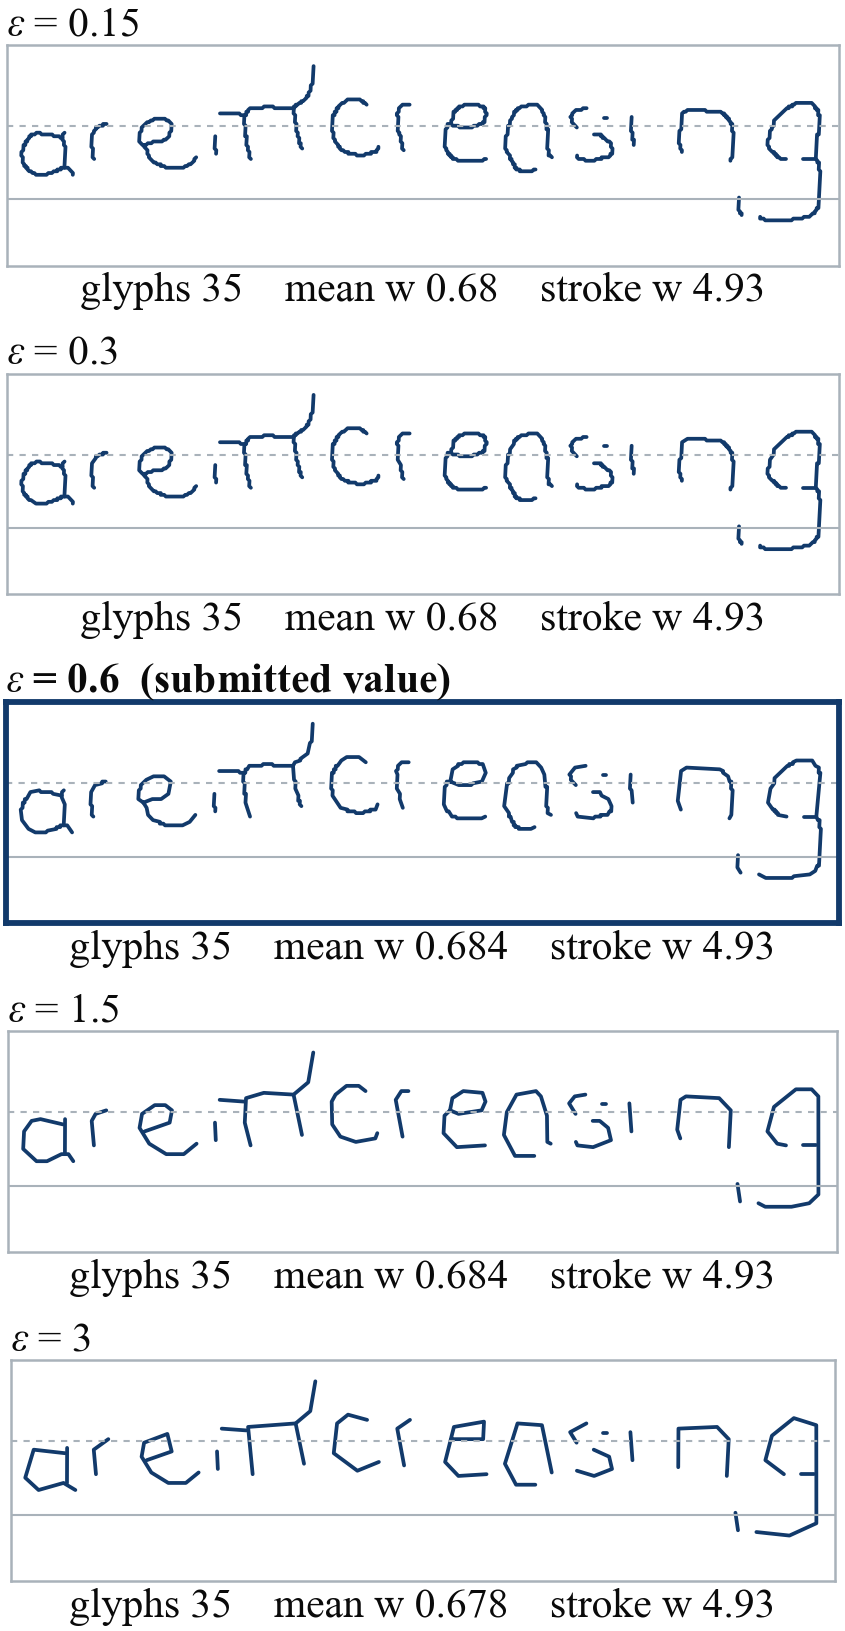
\includegraphics[width=\linewidth]{../figures/simplify_eps.png}

\caption{Douglas--Peucker tolerance for a stored stroke. Each panel is the same input processed by the submitted code with only $\varepsilon$ changed; the panel outlined in dark blue is the submitted value.}

\label{fig:simplify-eps}

\end{figure}

\begin{figure}[htbp]

\centering

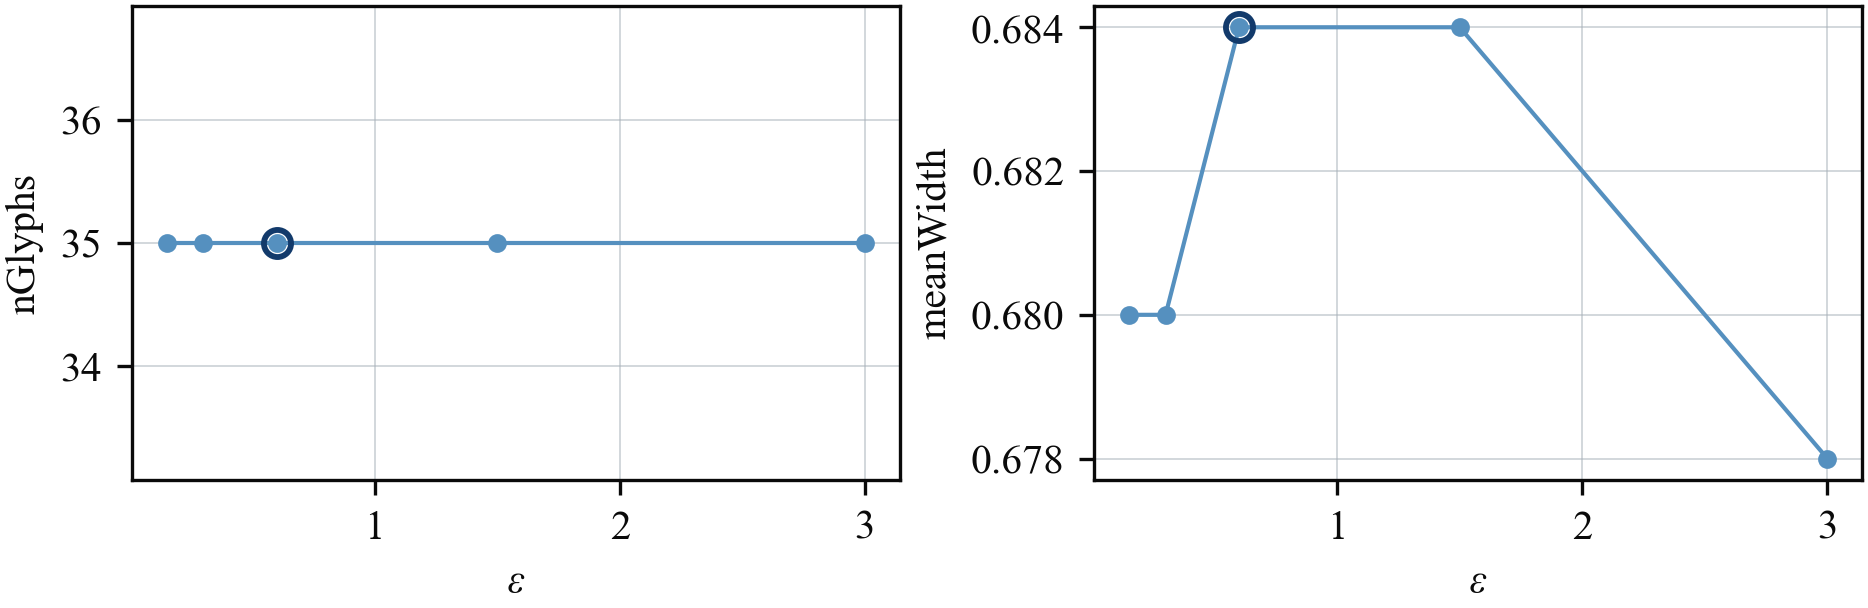
\includegraphics[width=\linewidth]{../figures/simplify_eps_trend.png}

\caption{Douglas--Peucker tolerance for a stored stroke: measured quantities against the swept value. The circled point is the submitted value.}

\end{figure}

\begin{table}[htbp]
\centering
\small
\caption{Douglas--Peucker tolerance for a stored stroke: measured effect of each swept value. The submitted value is in bold.}
\begin{tabular}{lrrrr}
\toprule
\$\textbackslash\{\}varepsilon\$ & \textsf{nGlyphs} & \textsf{meanWidth} & \textsf{strokeW} & \textsf{alignConf} \\
\midrule
0.15 & 35 & 0.68 & 4.93 & -0.045 \\
0.3 & 35 & 0.68 & 4.93 & -0.045 \\
\bfseries 0.6 & \bfseries 35 & \bfseries 0.684 & \bfseries 4.93 & \bfseries -0.045 \\
1.5 & 35 & 0.684 & 4.93 & -0.045 \\
3 & 35 & 0.678 & 4.93 & -0.045 \\
\bottomrule
\end{tabular}
\end{table}

\subsection{Weight on how high the ink reaches in the cut-cost profile}

\label{coef:cut-cost-top}

\begin{description}[leftmargin=5.2em,style=sameline]

\item[Symbol] $w_{\text{top}}$

\item[Value] \texttt{1.15}

\item[Source] \texttt{style.py}, \texttt{ExtractLineGlyphs}

\item[Swept] \texttt{0.0}, \texttt{0.5}, \texttt{1.15}, \texttt{2.5}, \texttt{5.0}

\end{description}

\paragraph{Basis}

Cutting a word into characters at columns of least ink is the classical vertical-projection segmentation of cursive script \cite{likforman2007,vinciarelli2001}.

\paragraph{Why this value}

The reader's alignment gives an approximate column for each character boundary; the boundary is then snapped to the cheapest nearby column. The cost has two parts: how much ink the column carries, and how high that ink reaches above the baseline. The second term exists because a column may be thin and still be a bad place to cut: the thin part of an \texttt{o} near its top, or an ascender, is thin but is in the middle of a letter. A good cut is through the \emph{low} ligature between letters. $w_{\text{top}} = 1.15$ makes a column whose ink reaches one x-height cost slightly more than a column carrying the typical amount of ink, so height and thinness are weighed about equally.

\paragraph{What the coefficient does}

\texttt{thin} is normalised by the $60$th percentile of non-zero column sums, so it is about $1.0$ for a typical inked column, and \texttt{topAbove} is clipped to $[0,3]$ x-heights. At $w_{\text{top}} = 0$ the cut is decided by ink alone and will happily slice through the top of a letter; at $5.0$ it is decided almost entirely by height and ignores how much ink it is cutting through.

\paragraph{Alternatives considered}

Cutting at the CTC alignment column directly with no snap, which leaves boundaries mid-stroke; or a full segmentation-free approach where glyphs are never cut out, which would mean giving up the per-letter store the synthesis depends on.

\paragraph{Worked example}

A column with the typical ink and no ink above the baseline costs about $1.0$; a column with half the typical ink reaching one x-height costs $0.5+1.15 = 1.65$, so the thinner but taller column is the worse cut.

\paragraph{What the sweep actually showed}

Nearly flat: $35$ glyphs at every value, and the mean stored width moves only from $0.690$ at $w_{\text{top}} = 0$ to $0.684$ everywhere else. In other words, on this line the ink term alone already picks essentially the same cut columns as the full cost, and the height term is confirming a decision rather than changing it. The one value that differs is $0$, which is the setting where the height term is removed entirely, so the sweep does show the term doing something --- just very little on a line this well separated. A cursive line with ligatures running at mid-height would be the test that matters.

\begin{figure}[htbp]

\centering

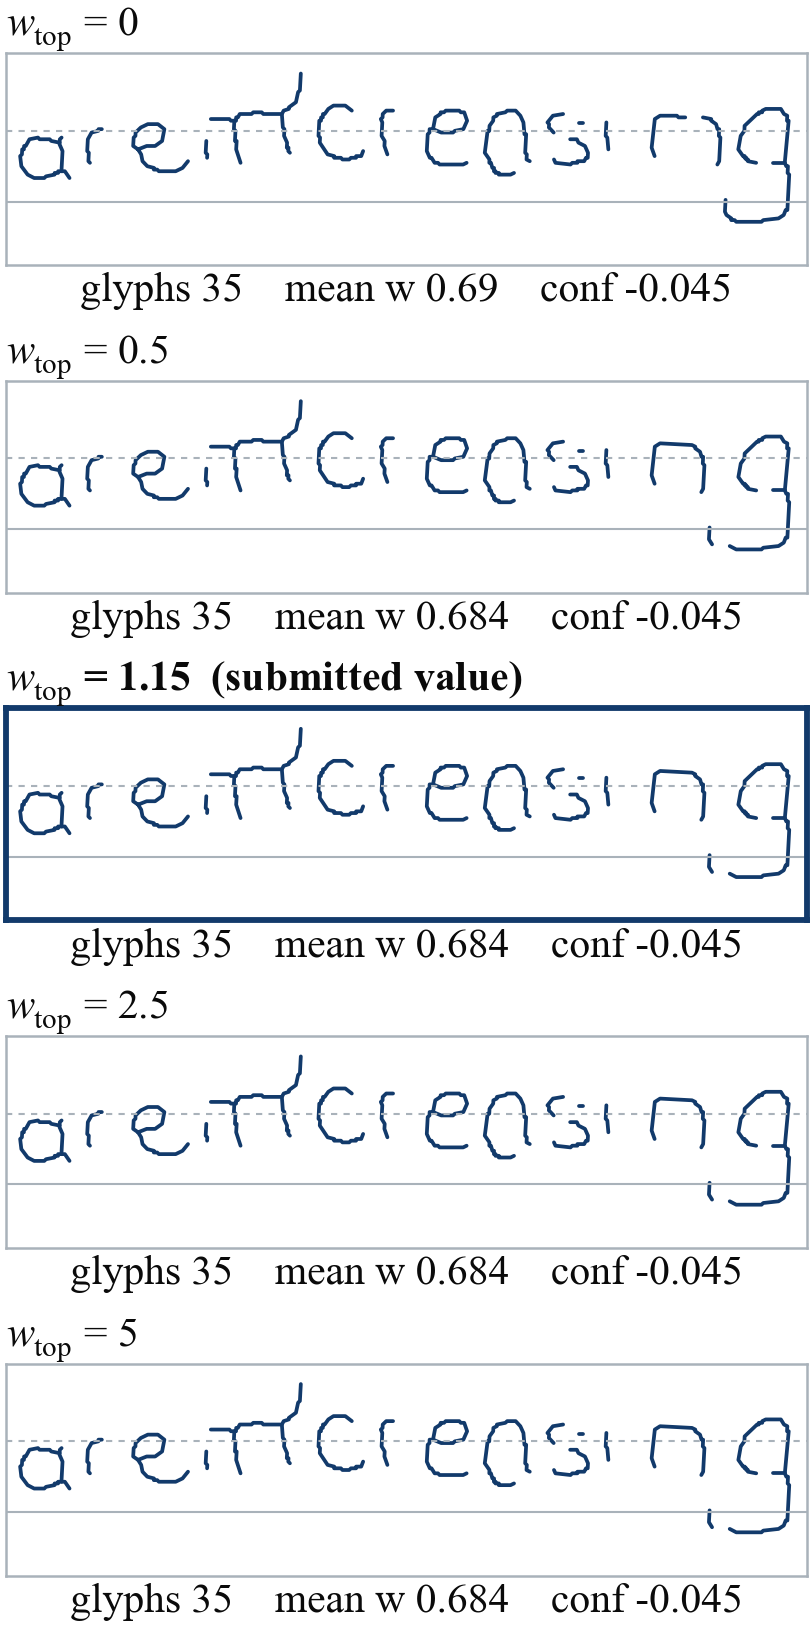
\includegraphics[width=\linewidth]{../figures/cut_cost_top.png}

\caption{Weight on how high the ink reaches in the cut-cost profile. Each panel is the same input processed by the submitted code with only $w_{\text{top}}$ changed; the panel outlined in dark blue is the submitted value.}

\label{fig:cut-cost-top}

\end{figure}

\begin{figure}[htbp]

\centering

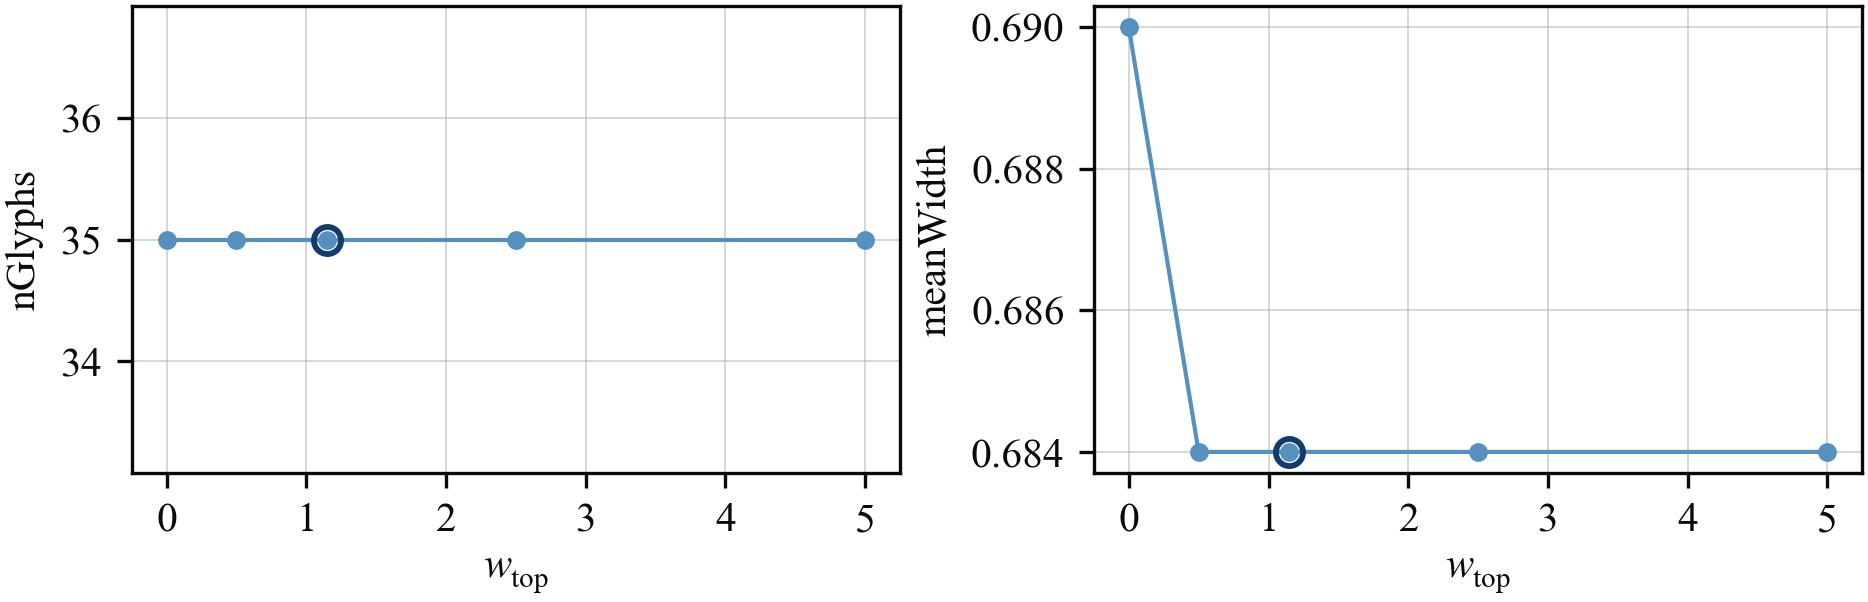
\includegraphics[width=\linewidth]{../figures/cut_cost_top_trend.png}

\caption{Weight on how high the ink reaches in the cut-cost profile: measured quantities against the swept value. The circled point is the submitted value.}

\end{figure}

\begin{table}[htbp]
\centering
\small
\caption{Weight on how high the ink reaches in the cut-cost profile: measured effect of each swept value. The submitted value is in bold.}
\begin{tabular}{lrrr}
\toprule
\$w\_\{\textbackslash\{\}text\{top\}\}\$ & \textsf{nGlyphs} & \textsf{meanWidth} & \textsf{alignConf} \\
\midrule
0 & 35 & 0.69 & -0.045 \\
0.5 & 35 & 0.684 & -0.045 \\
\bfseries 1.15 & \bfseries 35 & \bfseries 0.684 & \bfseries -0.045 \\
2.5 & 35 & 0.684 & -0.045 \\
5 & 35 & 0.684 & -0.045 \\
\bottomrule
\end{tabular}
\end{table}

\subsection{How far a character boundary may be moved to find a cheap column}

\label{coef:snap-radius}

\begin{description}[leftmargin=5.2em,style=sameline]

\item[Symbol] $r_{\text{snap}}$

\item[Value] \texttt{0.5}

\item[Source] \texttt{style.py}, \texttt{ExtractLineGlyphs}

\item[Swept] \texttt{0.1}, \texttt{0.25}, \texttt{0.5}, \texttt{0.9}, \texttt{1.5}

\end{description}

\paragraph{Basis}

Refining an approximate segmentation point by local search over a cost profile is standard in segmentation-based handwriting recognition \cite{likforman2007}.

\paragraph{Why this value}

The CTC alignment is accurate to a few frames, and one frame is four canvas columns, which after the canvas-to-pixel mapping is a noticeable fraction of a letter. The snap radius must therefore be large enough to reach the true ligature from the aligned guess, and small enough that the boundary cannot run into the neighbouring letter. Half an x-height is about half a letter width, which bounds the move to within the letter it belongs to.

\paragraph{What the coefficient does}

The search minimises $\text{cutCost} + 0.6\,|x-x_0|/r$, so there is a mild pull back towards the aligned guess: a far-away column must be clearly cheaper to win. Boundaries are also forced to be strictly increasing with a minimum cell of $0.08\,x_h$, so a large radius cannot collapse two boundaries onto one column.

\paragraph{Alternatives considered}

No snap at all, or a snap to the nearest column of zero ink, which does not exist inside a cursive word.

\paragraph{Worked example}

At $x_h = 42$ px, $r_{\text{snap}} = 21$ px, and one CTC frame maps to $2170/160 = 13.6$ px of the original crop, so the snap can correct an alignment error of about $1.5$ frames.

\paragraph{What the sweep actually showed}

The clearest effect in the glyph-cutting group. The number of glyphs kept falls $40$, $38$, $35$, $30$, $30$ as the radius grows, while their mean stored width rises $0.595$, $0.625$, $0.684$, $0.804$, $0.804$. The mechanism is visible in those two numbers together: a larger radius lets a boundary travel further from the aligned guess, cells become wider and more uneven, and more of the resulting glyphs are then rejected by the width and class filters. A smaller radius keeps more glyphs but they are narrower, which is the boundary sitting where the alignment put it rather than at a real gap. The submitted $0.5$ is in the middle of that trade and the sweep does not identify an optimum; measuring one needs ground-truth character boundaries, which this project does not have.

\begin{figure}[htbp]

\centering

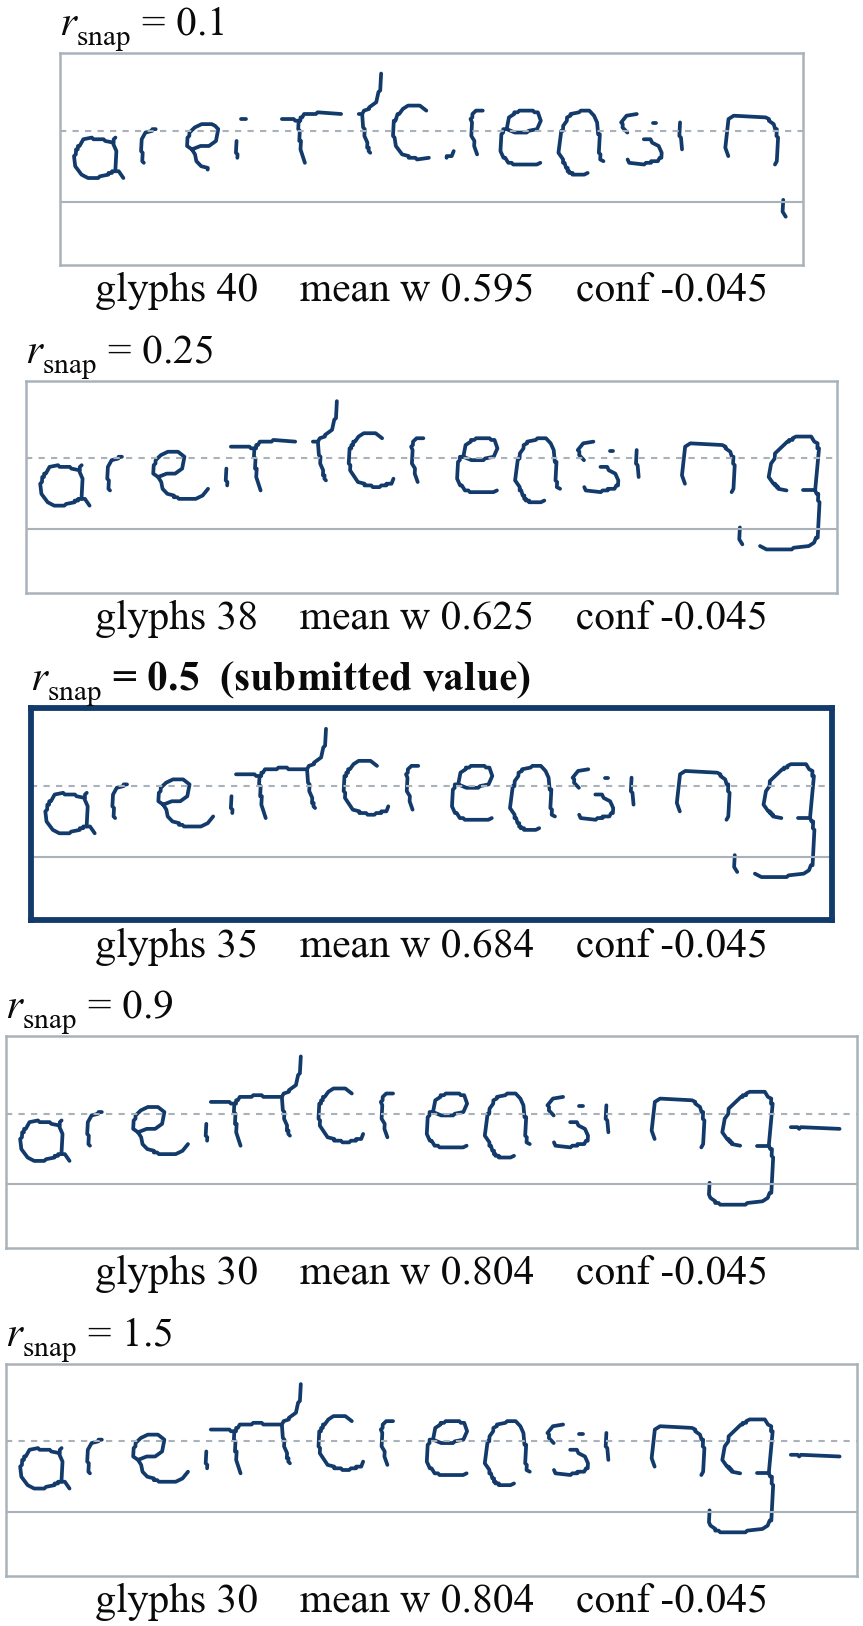
\includegraphics[width=\linewidth]{../figures/snap_radius.png}

\caption{How far a character boundary may be moved to find a cheap column. Each panel is the same input processed by the submitted code with only $r_{\text{snap}}$ changed; the panel outlined in dark blue is the submitted value.}

\label{fig:snap-radius}

\end{figure}

\begin{figure}[htbp]

\centering

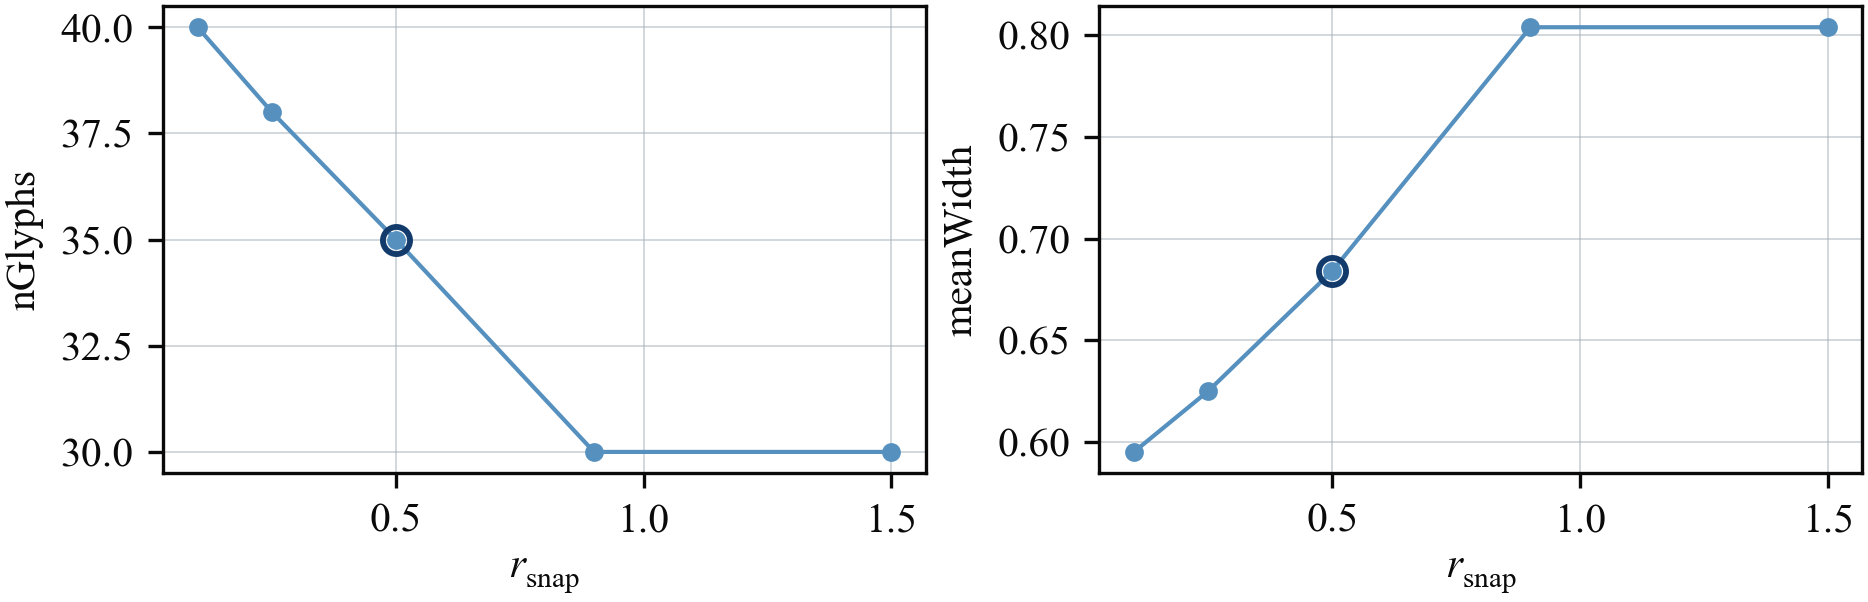
\includegraphics[width=\linewidth]{../figures/snap_radius_trend.png}

\caption{How far a character boundary may be moved to find a cheap column: measured quantities against the swept value. The circled point is the submitted value.}

\end{figure}

\begin{table}[htbp]
\centering
\small
\caption{How far a character boundary may be moved to find a cheap column: measured effect of each swept value. The submitted value is in bold.}
\begin{tabular}{lrrr}
\toprule
\$r\_\{\textbackslash\{\}text\{snap\}\}\$ & \textsf{nGlyphs} & \textsf{meanWidth} & \textsf{alignConf} \\
\midrule
0.1 & 40 & 0.595 & -0.045 \\
0.25 & 38 & 0.625 & -0.045 \\
\bfseries 0.5 & \bfseries 35 & \bfseries 0.684 & \bfseries -0.045 \\
0.9 & 30 & 0.804 & -0.045 \\
1.5 & 30 & 0.804 & -0.045 \\
\bottomrule
\end{tabular}
\end{table}

\subsection{Smallest cell a character boundary pair may enclose}

\label{coef:min-cell}

\begin{description}[leftmargin=5.2em,style=sameline]

\item[Symbol] $c_{\min}$

\item[Value] \texttt{0.08}

\item[Source] \texttt{style.py}, \texttt{ExtractLineGlyphs}

\item[Swept] \texttt{0.01}, \texttt{0.04}, \texttt{0.08}, \texttt{0.2}, \texttt{0.4}

\end{description}

\paragraph{Basis}

Monotonic, non-degenerate boundaries are a requirement of any segmentation that must produce one region per label \cite{likforman2007}; the CTC alignment that supplies the guesses is itself monotonic \cite[p.~370]{graves2006}.

\paragraph{Why this value}

Boundaries are built into one shared, strictly increasing array precisely so that two neighbouring boundaries cannot land on the same column and leave a character with an empty cell. $c_{\min}$ is the width that guarantees it, and it must also leave room for every remaining character, which is why the upper limit for boundary $k$ is $\text{bnd}[n]-(n-k)c_{\min}$. At $0.08$ x-heights a cell is at least a few pixels wide, enough to hold the thinnest real mark, such as the stem of an \texttt{l} or a full stop.

\paragraph{What the coefficient does}

Raising $c_{\min}$ forces cells apart and so forces boundaries away from where the cost profile wants them, eventually overriding the snap entirely and producing an evenly spaced comb. Lowering it allows very narrow cells, whose glyphs are then rejected downstream for being too thin.

\paragraph{Worked example}

At $x_h = 42$ px, $c_{\min} = 3.4$ px. For a line of $48$ characters the boundaries must span at least $48 \times 3.4 = 161$ px, against a crop width of $2170$ px, so the constraint is slack on a normal line.

\paragraph{What the sweep actually showed}

Flat at $35$ glyphs for every value from $0.01$ to $0.20$, with $36$ glyphs and a slightly smaller mean width at $0.40$. The constraint is simply slack on an ordinary line: $48$ characters at $c_{\min} = 0.08$ need $161$ px of the $2\,170$ px crop, so the boundaries are nowhere near being forced apart. The coefficient is a guard against a degenerate case --- two boundaries landing on one column --- and this line does not produce that case, so the null result is the expected one.

\begin{figure}[htbp]

\centering

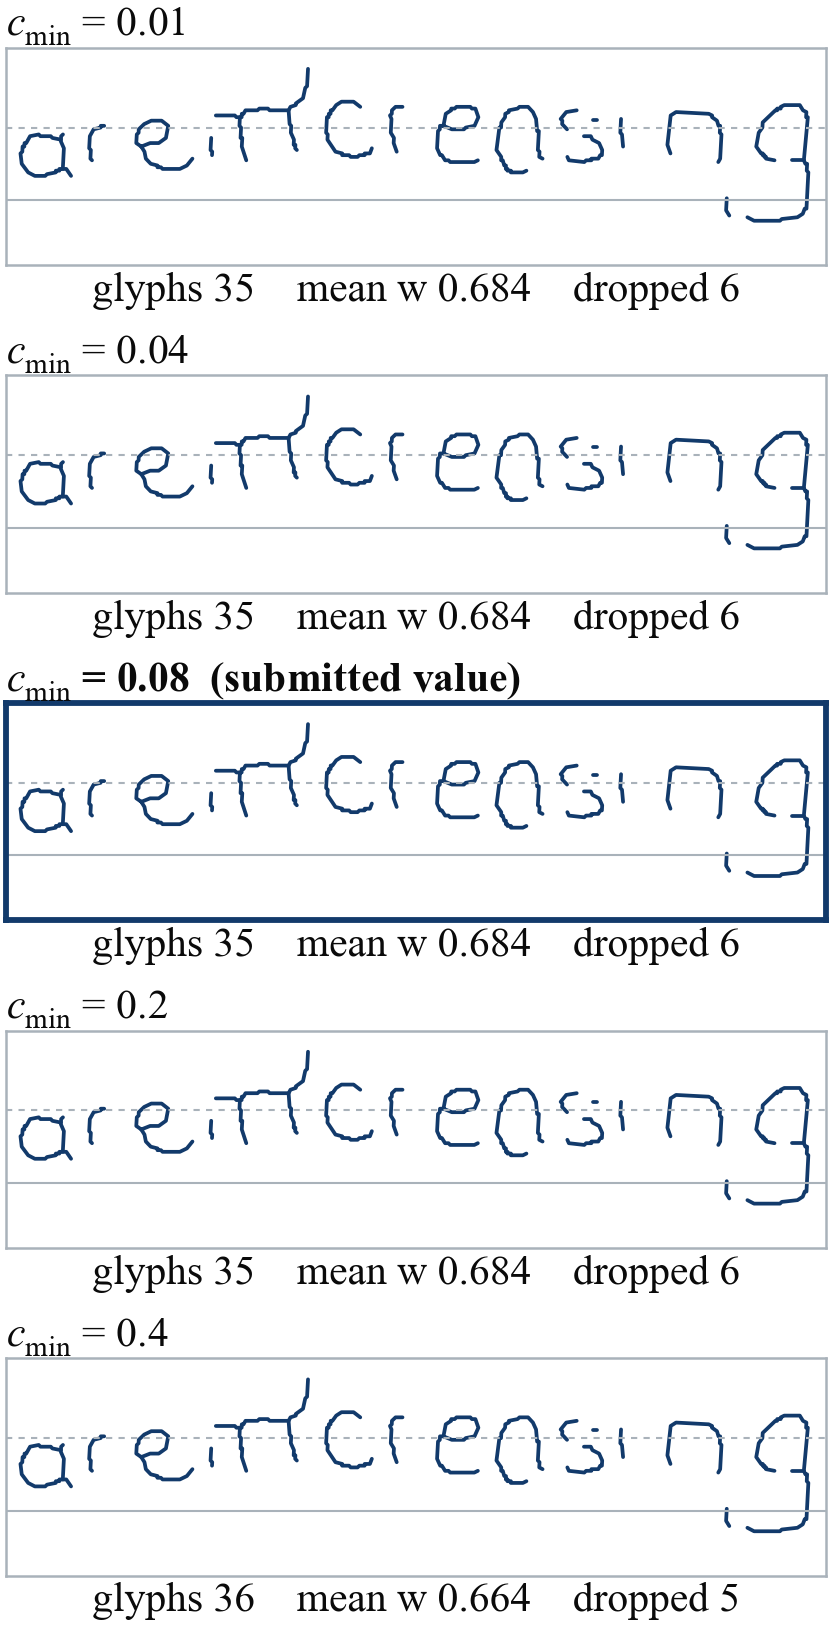
\includegraphics[width=\linewidth]{../figures/min_cell.png}

\caption{Smallest cell a character boundary pair may enclose. Each panel is the same input processed by the submitted code with only $c_{\min}$ changed; the panel outlined in dark blue is the submitted value.}

\label{fig:min-cell}

\end{figure}

\begin{figure}[htbp]

\centering

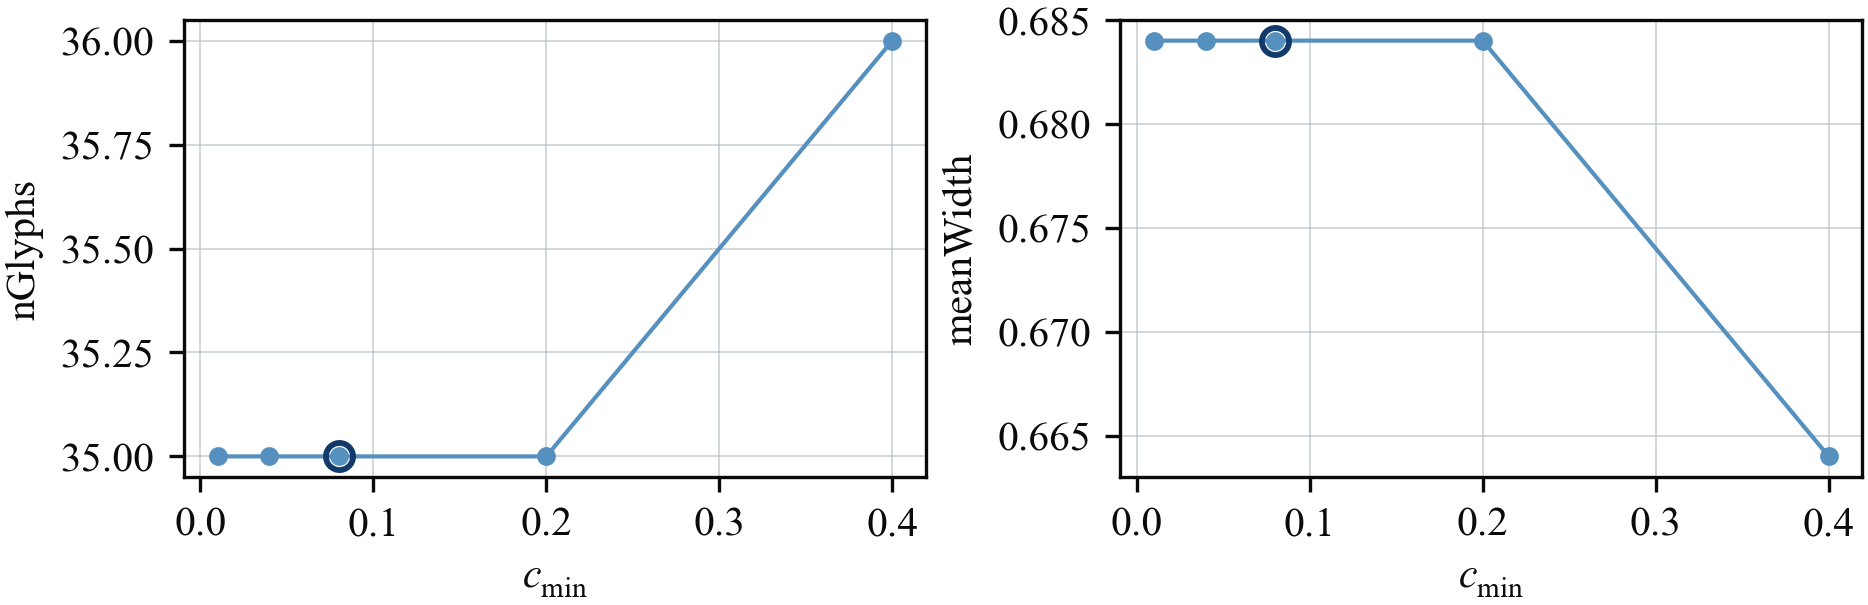
\includegraphics[width=\linewidth]{../figures/min_cell_trend.png}

\caption{Smallest cell a character boundary pair may enclose: measured quantities against the swept value. The circled point is the submitted value.}

\end{figure}

\begin{table}[htbp]
\centering
\small
\caption{Smallest cell a character boundary pair may enclose: measured effect of each swept value. The submitted value is in bold.}
\begin{tabular}{lrrr}
\toprule
\$c\_\{\textbackslash\{\}min\}\$ & \textsf{nGlyphs} & \textsf{meanWidth} & \textsf{nNone} \\
\midrule
0.01 & 35 & 0.684 & 6 \\
0.04 & 35 & 0.684 & 6 \\
\bfseries 0.08 & \bfseries 35 & \bfseries 0.684 & \bfseries 6 \\
0.2 & 35 & 0.684 & 6 \\
0.4 & 36 & 0.664 & 5 \\
\bottomrule
\end{tabular}
\end{table}

\section{Glyph filtering}

\subsection{Widest glyph accepted, in x-heights}

\label{coef:glyph-max-w}

\begin{description}[leftmargin=5.2em,style=sameline]

\item[Symbol] $W_{\text{glyph}}$

\item[Value] \texttt{2.1}

\item[Source] \texttt{style.py}, \texttt{MAX\_GLYPH\_W}

\item[Swept] \texttt{1.1}, \texttt{1.6}, \texttt{2.1}, \texttt{3.0}, \texttt{4.5}

\end{description}

\paragraph{Basis}

Width normalised by x-height is the scale-free measure of letter size used throughout handwriting analysis \cite{vinciarelli2001}; rejecting over-wide segmentation hypotheses is the standard guard in segmentation-based recognition \cite{likforman2007}.

\paragraph{Why this value}

A glyph is cut at the boundaries the reader's forced alignment suggests, and that alignment is sometimes wrong: a boundary placed too far right makes one cell swallow its neighbour. The resulting shape is then two letters stored under one character, which later draws as nonsense. Real lowercase letters are at most about one x-height wide and the widest, \texttt{m} and \texttt{w}, reach roughly $1.5$. A cell holding two letters is at least $2$ wide. $2.1$ sits above every single letter and at the bottom of the two-letter range, and the wide characters get their own larger limit of $2.9$ so they are not penalised for being wide.

\paragraph{What the coefficient does}

This is one of a battery of filters in \texttt{BuildAuthorProfile}, and it is the one that catches the specific failure of a swallowed neighbour. Raising it lets merged pairs into the store, which shows up later as a median prior distance that climbs, because a two-letter shape is nothing like the pooled prototype of its character.

\paragraph{Alternatives considered}

Rejecting on the alignment confidence alone, which is already done at line level by \texttt{ALIGN\_CONF\_PCT}, or comparing each glyph against the letter prior and rejecting outliers, which \texttt{PriorFilter} does as a later and softer stage.

\paragraph{Worked example}

At $x_h = 42$ px a glyph may be at most $2.1 \times 42 = 88$ px wide, against a cell advance that is typically $0.7$--$1.0$ x-heights.

\paragraph{What the sweep actually showed}

\textbf{The limit never fires at the submitted value on this data.} Rebuilding Owen's profile from 18 lines gives $35$ characters and $165$ variants at $W_{\text{glyph}} = 1.6$, $2.1$, $3.0$ and $4.5$ alike --- four identical results --- and only at $1.1$ does the limit bite, dropping to $33$ characters and $160$ variants. So no glyph cut from these lines is wider than $1.6$ x-heights, and the submitted $2.1$ sits well clear of anything the cutter actually produced. That is the correct behaviour for a safety net --- it should not be removing good glyphs --- but it means this sweep cannot show the limit catching the failure it exists for. Demonstrating that needs lines where the forced alignment is wrong enough to merge two letters into one cell, which these well-read lines do not provide.

\begin{figure}[htbp]

\centering

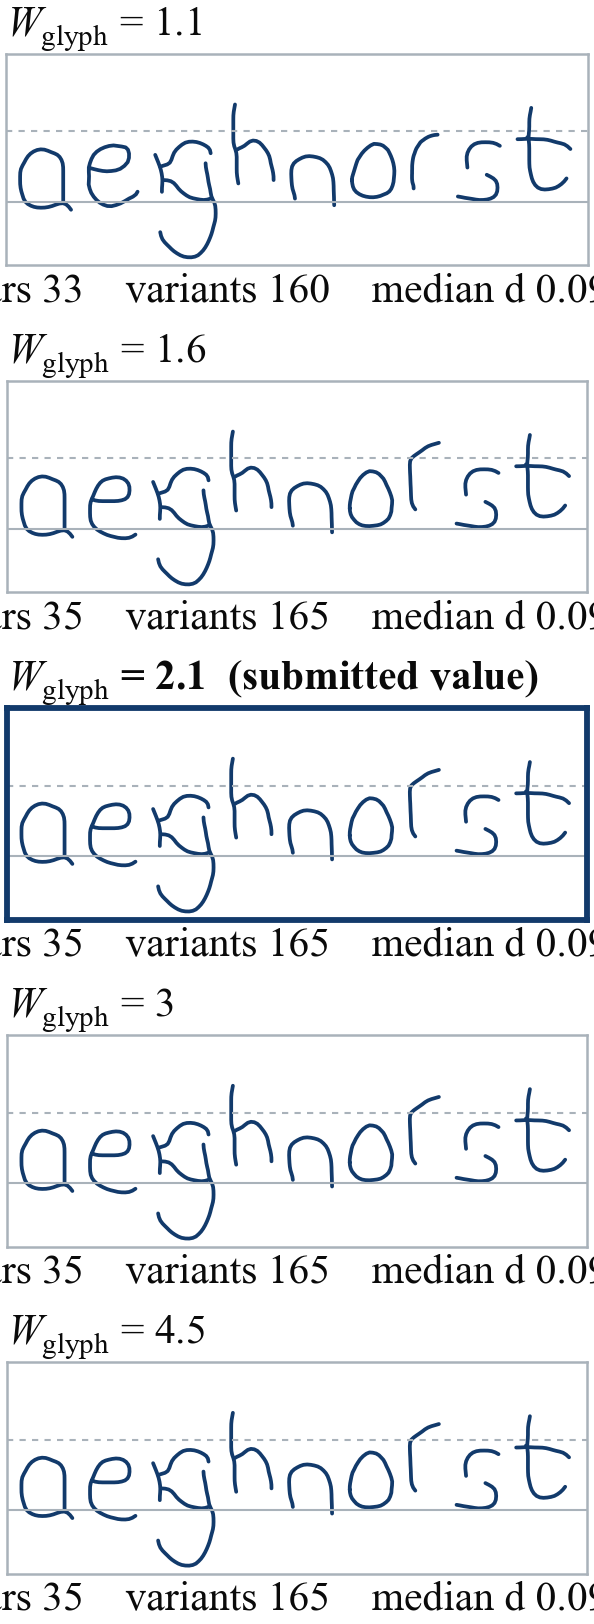
\includegraphics[width=\linewidth]{../figures/glyph_max_w.png}

\caption{Widest glyph accepted, in x-heights. Each panel is the same input processed by the submitted code with only $W_{\text{glyph}}$ changed; the panel outlined in dark blue is the submitted value.}

\label{fig:glyph-max-w}

\end{figure}

\begin{figure}[htbp]

\centering

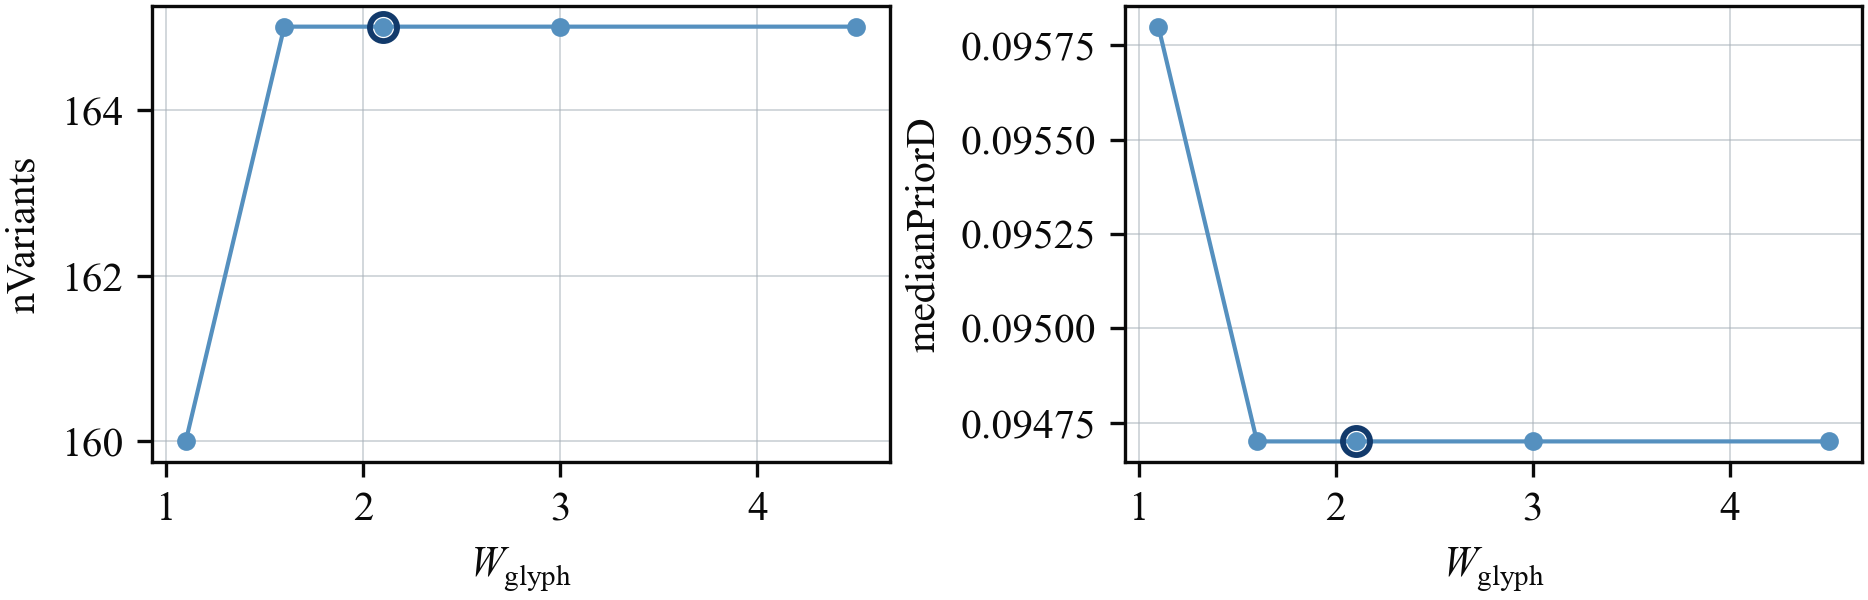
\includegraphics[width=\linewidth]{../figures/glyph_max_w_trend.png}

\caption{Widest glyph accepted, in x-heights: measured quantities against the swept value. The circled point is the submitted value.}

\end{figure}

\begin{table}[htbp]
\centering
\small
\caption{Widest glyph accepted, in x-heights: measured effect of each swept value. The submitted value is in bold.}
\begin{tabular}{lrrrr}
\toprule
\$W\_\{\textbackslash\{\}text\{glyph\}\}\$ & \textsf{nChars} & \textsf{nVariants} & \textsf{medianPriorD} & \textsf{connectedness} \\
\midrule
1.1 & 33 & 160 & 0.0958 & 0.231 \\
1.6 & 35 & 165 & 0.0947 & 0.231 \\
\bfseries 2.1 & \bfseries 35 & \bfseries 165 & \bfseries 0.0947 & \bfseries 0.231 \\
3 & 35 & 165 & 0.0947 & 0.231 \\
4.5 & 35 & 165 & 0.0947 & 0.231 \\
\bottomrule
\end{tabular}
\end{table}

\subsection{Side of the square occupancy descriptor}

\label{coef:shape-grid-n}

\begin{description}[leftmargin=5.2em,style=sameline]

\item[Symbol] $n_{\text{grid}}$

\item[Value] \texttt{12}

\item[Source] \texttt{style.py}, \texttt{\_ShapeGrid}

\item[Swept] \texttt{6}, \texttt{8}, \texttt{12}, \texttt{16}, \texttt{24}

\end{description}

\paragraph{Basis}

A normalised grid of ink occupancy is the classical shape descriptor for character matching \cite{barrow1977,dubuisson1994}; the square-root damping and blur follow the same reasoning as the gradient-histogram features used for writer identification \cite{bulacu2007}.

\paragraph{Why this value}

The descriptor exists to answer one question: how far is this glyph from the way this letter usually looks? It must therefore be coarse enough that two honest writings of the same letter match, and fine enough that a fragment or a merged pair does not. Each cell of a $12\times12$ grid is $1/12$ of the letter box, about $3.5$ px on a $42$ px x-height, so a stroke placed one cell differently still overlaps after the $3\times3$ blur that follows. Finer grids make two writings of the same letter disagree simply because the pen wavered; coarser ones stop distinguishing \texttt{c} from \texttt{e}.

\paragraph{What the coefficient does}

The descriptor is normalised to unit length and compared by dot product, so $n_{\text{grid}}$ changes the dimension of the space, $144$ at the submitted value. Distances are not comparable between grid sizes, which is why the sweep reports the median prior distance it produces rather than claiming one size scores better than another: a change in the median is partly a change of units.

\paragraph{Alternatives considered}

Hausdorff distance between point sets \cite{dubuisson1994}, which needs no grid but is dominated by outliers; chamfer matching \cite{barrow1977}; or resampling both strokes and comparing point by point, which \texttt{\_DenoisedPrototype} does for averaging but which needs the strokes to correspond.

\paragraph{Worked example}

The blur weights are $0.25$ at the centre and $0.09375$ at each of the eight neighbours, summing to $0.25+8 \times 0.09375 = 1.0$, so the blur preserves total ink before normalisation.

\paragraph{What the sweep actually showed}

The median prior distance rises steeply and monotonically with the grid size: $0.0209$, $0.0451$, $0.0947$, $0.1565$, $0.3183$ for $n = 6$, $8$, $12$, $16$, $24$, while the number of variants kept barely moves ($160$ to $169$). This is the clearest possible demonstration of the point made above, that \textbf{distances are not comparable between grid sizes}: a finer grid means two honest writings of the same letter overlap in fewer cells, so every distance grows, and the fifteen-fold spread here is mostly a change of units rather than a change in discrimination. It also shows the real design tension. At $n = 6$ the descriptor rates almost everything as typical, which makes the prior filter useless; at $n = 24$ it rates a writer's own letters as atypical of themselves, which makes it over-aggressive. $n = 12$ is between those, but this sweep cannot show it is the best point, because the quantity it reports is measured in different units at every value. A fair comparison would score each grid size by how well it separates correctly cut glyphs from known-bad ones, and that needs labelled bad cuts, which do not exist in this project.

\begin{figure}[htbp]

\centering

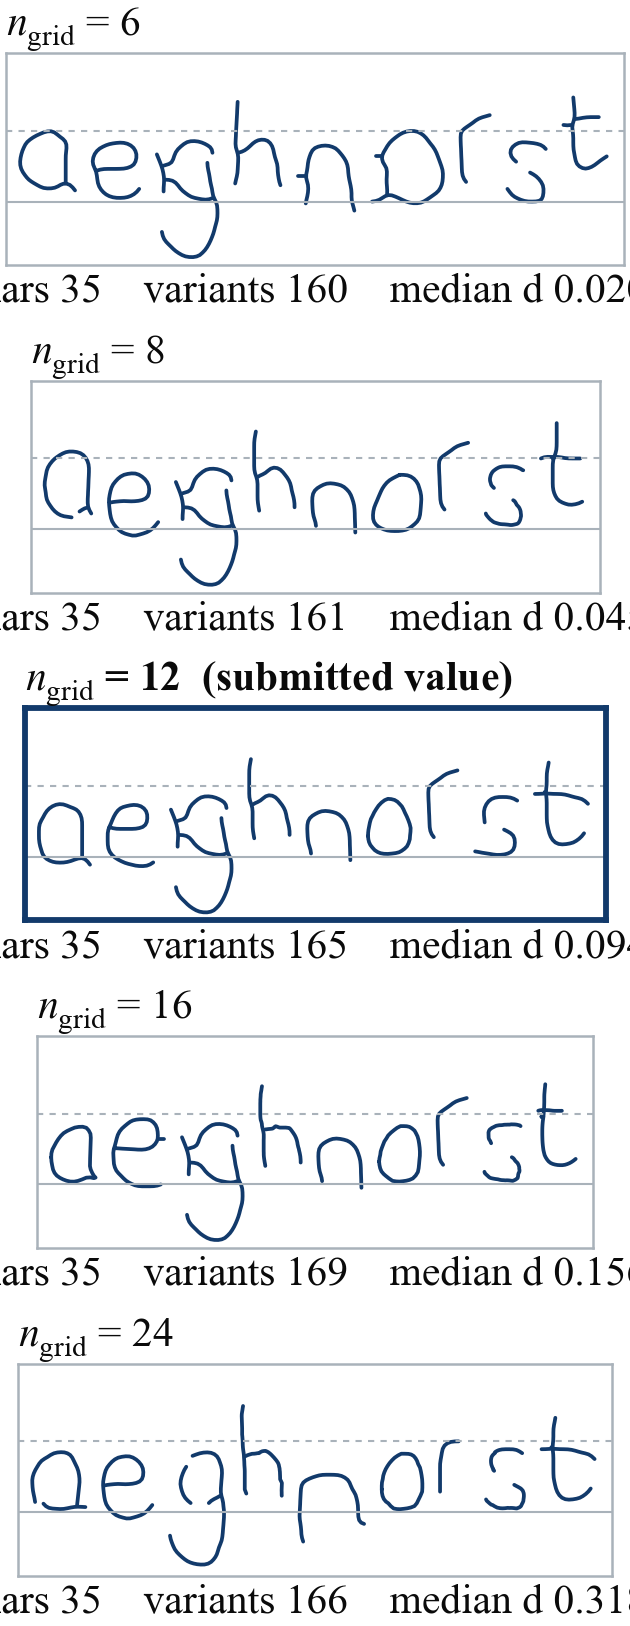
\includegraphics[width=\linewidth]{../figures/shape_grid_n.png}

\caption{Side of the square occupancy descriptor. Each panel is the same input processed by the submitted code with only $n_{\text{grid}}$ changed; the panel outlined in dark blue is the submitted value.}

\label{fig:shape-grid-n}

\end{figure}

\begin{figure}[htbp]

\centering

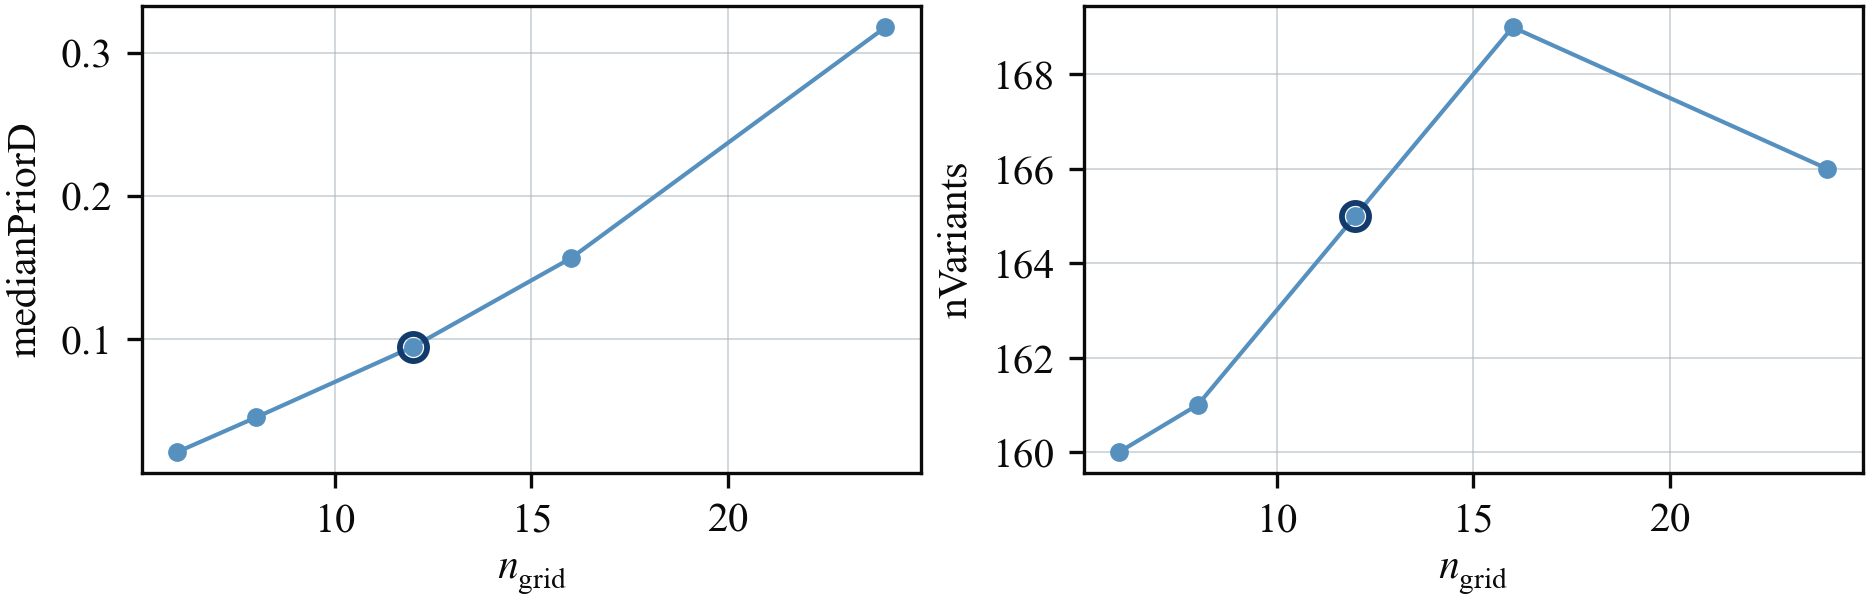
\includegraphics[width=\linewidth]{../figures/shape_grid_n_trend.png}

\caption{Side of the square occupancy descriptor: measured quantities against the swept value. The circled point is the submitted value.}

\end{figure}

\begin{table}[htbp]
\centering
\small
\caption{Side of the square occupancy descriptor: measured effect of each swept value. The submitted value is in bold.}
\begin{tabular}{lrrr}
\toprule
\$n\_\{\textbackslash\{\}text\{grid\}\}\$ & \textsf{nChars} & \textsf{nVariants} & \textsf{medianPriorD} \\
\midrule
6 & 35 & 160 & 0.0209 \\
8 & 35 & 161 & 0.0451 \\
\bfseries 12 & \bfseries 35 & \bfseries 165 & \bfseries 0.0947 \\
16 & 35 & 169 & 0.1565 \\
24 & 35 & 166 & 0.3183 \\
\bottomrule
\end{tabular}
\end{table}

\section{Profile building}

\subsection{Reading-confidence percentile below which a whole line is not trusted}

\label{coef:align-conf-pct}

\begin{description}[leftmargin=5.2em,style=sameline]

\item[Symbol] $q_{\text{conf}}$

\item[Value] \texttt{25}

\item[Source] \texttt{style.py}, \texttt{ALIGN\_CONF\_PCT}

\item[Swept] \texttt{0}, \texttt{10}, \texttt{25}, \texttt{50}, \texttt{75}

\end{description}

\paragraph{Basis}

The confidence is the mean per-frame log probability of the forced alignment path \cite[pp.~370--372]{graves2006}; discarding low-confidence training material is standard practice in semi-supervised and self-labelled recognition pipelines \cite{wigington2017}.

\paragraph{Why this value}

Glyph boundaries are only as good as the alignment that produced them, and the alignment is poor where the crop is poor: a line cut badly, a line the writer struck through, a line with an unreadable word. Those lines would contribute wrongly cut glyphs to the store. A \emph{relative} limit is used rather than an absolute log probability because confidence depends on the writer and on line length; discarding the worst quarter of a writer's own lines is a statement about that writer's pages, not about an absolute scale. It is applied only when there are at least eight lines, since a quartile of fewer is meaningless.

\paragraph{What the coefficient does}

At $q_{\text{conf}} = 0$ nothing is discarded; at $75$ only the best quarter of lines contributes, which gives cleaner glyphs but far fewer of them, and some characters then fall below the minimum variant count and disappear from the store entirely. The trade is coverage against cleanliness, and the sweep reports both: variants kept, and their median prior distance.

\paragraph{Alternatives considered}

An absolute confidence floor, which would need recalibrating per checkpoint; or weighting glyphs by confidence instead of discarding lines, which the later filters partly achieve.

\paragraph{Worked example}

With $18$ lines, discarding the lowest quartile removes the four or five worst-read lines before any glyph is stored.

\begin{figure}[htbp]

\centering

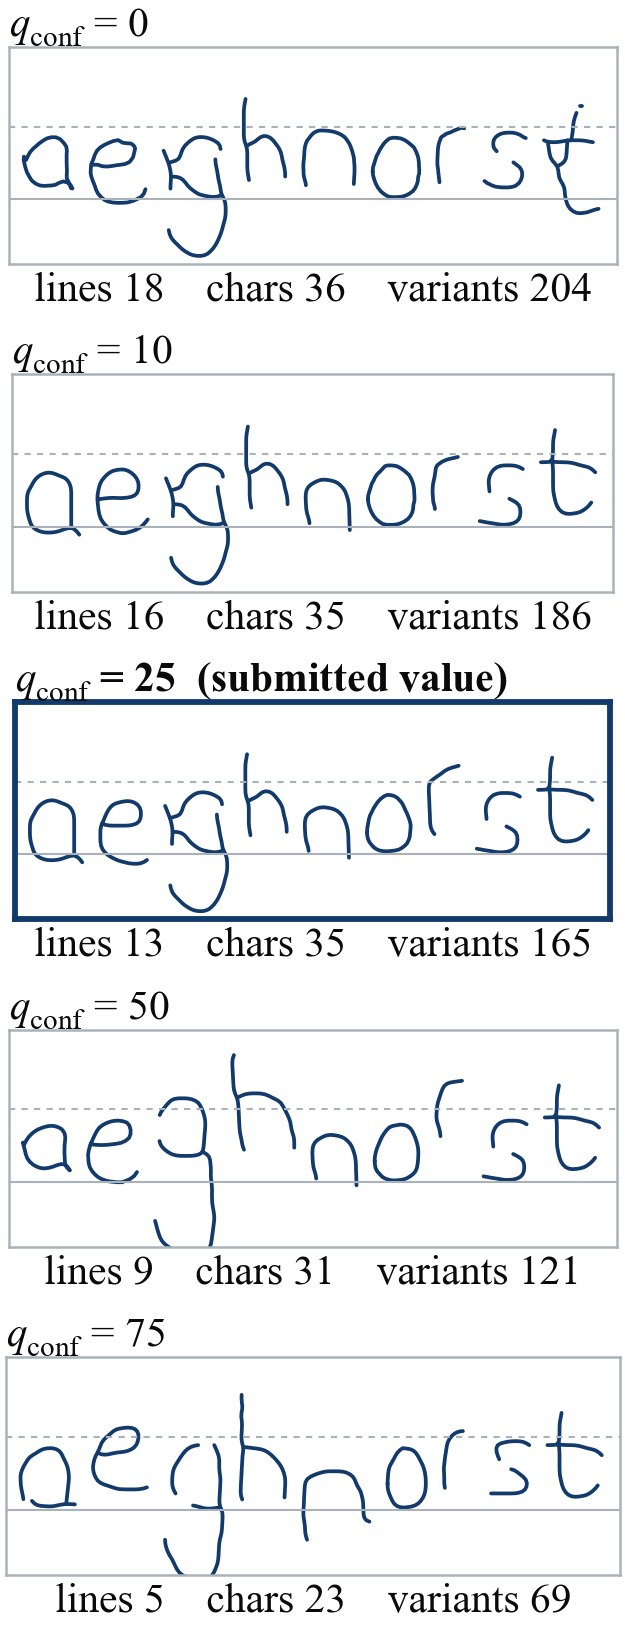
\includegraphics[width=\linewidth]{../figures/align_conf_pct.png}

\caption{Reading-confidence percentile below which a whole line is not trusted. Each panel is the same input processed by the submitted code with only $q_{\text{conf}}$ changed; the panel outlined in dark blue is the submitted value.}

\label{fig:align-conf-pct}

\end{figure}

\begin{figure}[htbp]

\centering

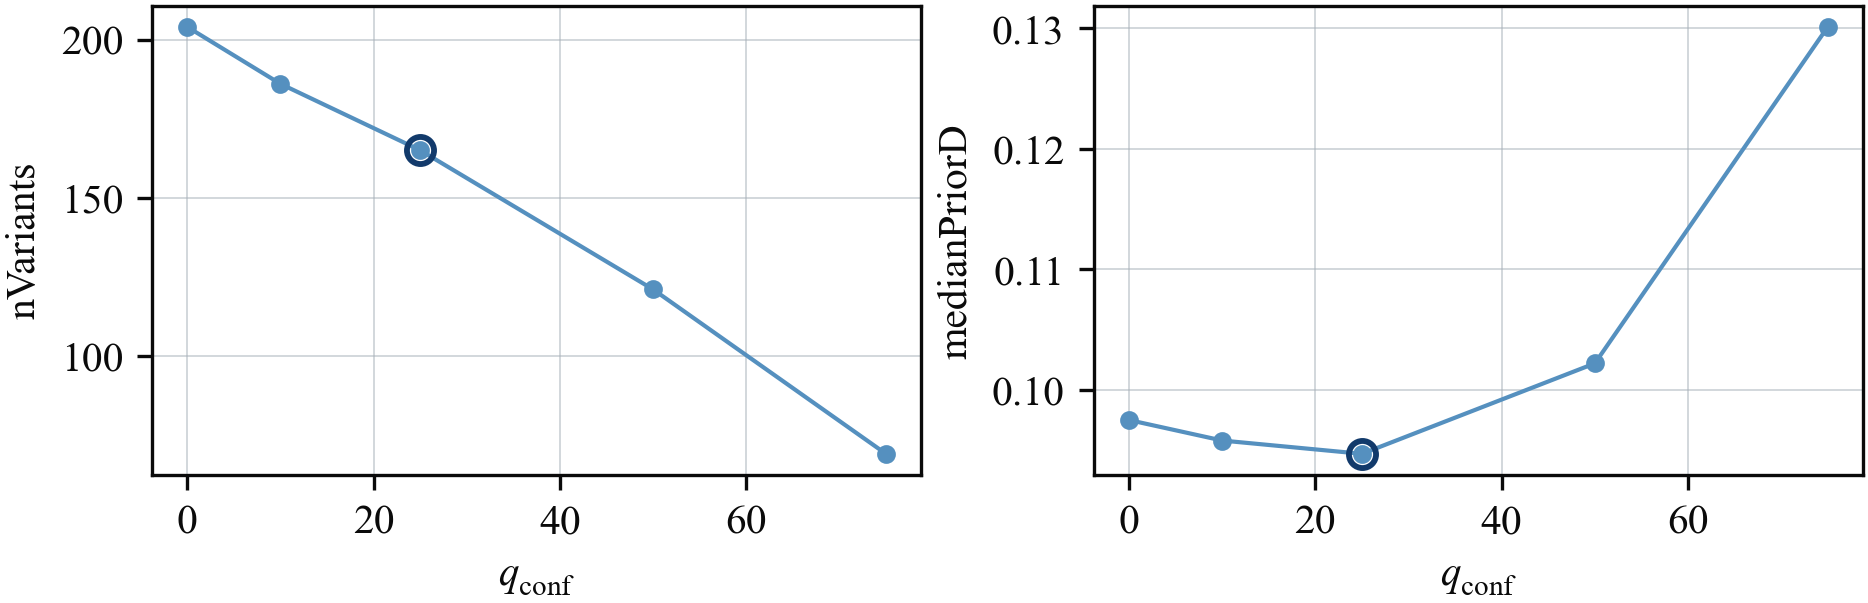
\includegraphics[width=\linewidth]{../figures/align_conf_pct_trend.png}

\caption{Reading-confidence percentile below which a whole line is not trusted: measured quantities against the swept value. The circled point is the submitted value.}

\end{figure}

\begin{table}[htbp]
\centering
\small
\caption{Reading-confidence percentile below which a whole line is not trusted: measured effect of each swept value. The submitted value is in bold.}
\begin{tabular}{lrrrr}
\toprule
\$q\_\{\textbackslash\{\}text\{conf\}\}\$ & \textsf{nLines} & \textsf{nChars} & \textsf{nVariants} & \textsf{medianPriorD} \\
\midrule
0 & 18 & 36 & 204 & 0.0975 \\
10 & 16 & 35 & 186 & 0.0958 \\
\bfseries 25 & \bfseries 13 & \bfseries 35 & \bfseries 165 & \bfseries 0.0947 \\
50 & 9 & 31 & 121 & 0.1022 \\
75 & 5 & 23 & 69 & 0.1301 \\
\bottomrule
\end{tabular}
\end{table}

\subsection{Shapes of one letter kept per writer}

\label{coef:max-variants}

\begin{description}[leftmargin=5.2em,style=sameline]

\item[Symbol] $V_{\max}$

\item[Value] \texttt{12}

\item[Source] \texttt{style.py}, \texttt{MAX\_VARIANTS\_PER\_CHAR}

\item[Swept] \texttt{2}, \texttt{5}, \texttt{12}, \texttt{25}, \texttt{60}

\end{description}

\paragraph{Basis}

Storing several exemplars per character and choosing among them at synthesis time is the allographic model of handwriting: a writer has a repertoire of forms per letter rather than one \cite{schomaker1990}, and natural variation between repetitions is intrinsic to the motor process \cite{plamondon2000}.

\paragraph{Why this value}

One shape per letter gives output in which every \texttt{e} is identical, which no reader accepts as handwriting. Keeping every shape instead means keeping the badly cut ones too, and makes the profile large. $12$ is set above the number needed for the repetition not to be visible within a line: an ordinary line holds a few instances of the commonest letters, so a dozen forms means a letter rarely repeats its exact shape on one line. The variants are sorted by typicality first, so the cut keeps the best twelve, and the synthesis then draws from only the top $5$ of them with a decreasing weight.

\paragraph{What the coefficient does}

Because \texttt{\_ELIGIBLE\_VARIANTS} is $5$, raising $V_{\max}$ beyond $5$ changes the stored profile size without changing what is usually drawn; it matters mainly for the medoid and prototype calculations, which pool all kept variants. Lowering it below $5$ directly reduces the variety the synthesis can draw on.

\paragraph{Alternatives considered}

Clustering the variants and keeping one exemplar per cluster, which is closer to the allographic account \cite{schomaker1990} but needs a cluster count; or keeping all and selecting at draw time, which is what the eligibility limit approximates.

\paragraph{Worked example}

Owen's profile holds $43$ characters and $307$ variants at the submitted setting, an average of $7.1$ per character, so the cap binds only for the commonest letters.

\begin{figure}[htbp]

\centering

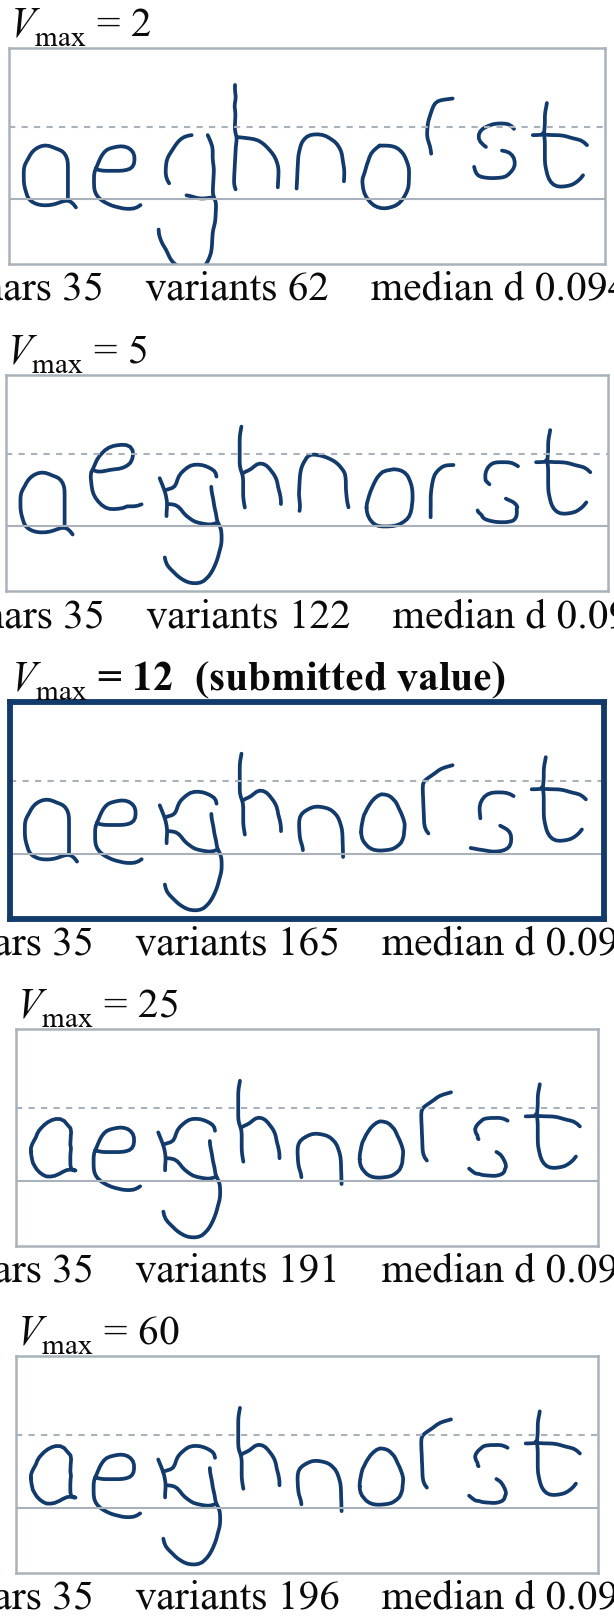
\includegraphics[width=\linewidth]{../figures/max_variants.png}

\caption{Shapes of one letter kept per writer. Each panel is the same input processed by the submitted code with only $V_{\max}$ changed; the panel outlined in dark blue is the submitted value.}

\label{fig:max-variants}

\end{figure}

\begin{figure}[htbp]

\centering

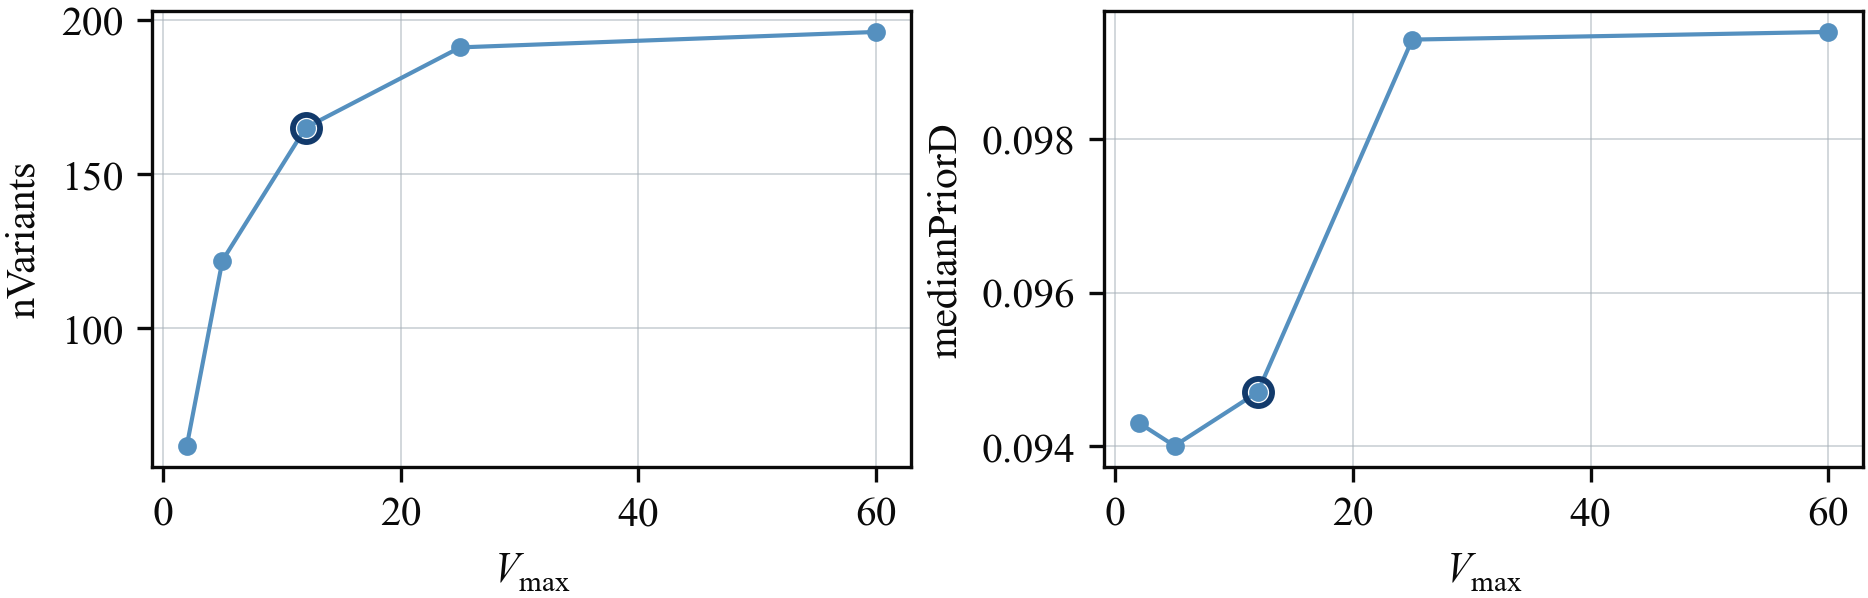
\includegraphics[width=\linewidth]{../figures/max_variants_trend.png}

\caption{Shapes of one letter kept per writer: measured quantities against the swept value. The circled point is the submitted value.}

\end{figure}

\begin{table}[htbp]
\centering
\small
\caption{Shapes of one letter kept per writer: measured effect of each swept value. The submitted value is in bold.}
\begin{tabular}{lrrr}
\toprule
\$V\_\{\textbackslash\{\}max\}\$ & \textsf{nChars} & \textsf{nVariants} & \textsf{medianPriorD} \\
\midrule
2 & 35 & 62 & 0.0943 \\
5 & 35 & 122 & 0.094 \\
\bfseries 12 & \bfseries 35 & \bfseries 165 & \bfseries 0.0947 \\
25 & 35 & 191 & 0.0993 \\
60 & 35 & 196 & 0.0994 \\
\bottomrule
\end{tabular}
\end{table}

\section{Synthesis: joining}

\subsection{Joinedness below which a hand is drawn as print and makes no joins}

\label{coef:join-conn-floor}

\begin{description}[leftmargin=5.2em,style=sameline]

\item[Symbol] $c_{\text{print}}$

\item[Value] \texttt{0.45}

\item[Source] \texttt{synthesise.py}, \texttt{JOIN\_PRINT\_CONN\_FLOOR}

\item[Swept] \texttt{0.0}, \texttt{0.25}, \texttt{0.45}, \texttt{0.65}, \texttt{0.95}

\end{description}

\paragraph{Basis}

Whether a hand joins its letters is one of the standard descriptors of writing style and is used directly as a writer-identification feature \cite{bulacu2007}; the connected-versus-print distinction is basic to handwriting analysis \cite{plamondon2000}.

\paragraph{Why this value}

The profile measures \texttt{connectedness} as the share of adjacent in-word letter pairs whose centrelines actually crossed the boundary between them, so it is an observed property of the writer, between $0$ and $1$. It is then used as a probability: each pair is joined with that chance. A hand that joins occasionally, say one pair in five, is not a joining hand, and drawing random ligatures into a print hand looks worse than drawing none, because the join appears in arbitrary places. The floor forces the probability to exactly zero below $c_{\text{print}}$ rather than letting it taper. $0.45$ is below the middle of the range and above the measured connectedness of the clear print hands in this set.

\paragraph{What the coefficient does}

This is a threshold on a measured quantity, so its effect is a step, not a gradient, and which side a given writer falls on is what matters. Owen measures $0.319$, so at the submitted setting Owen is drawn as a print hand with no joins at all; at $c_{\text{print}} = 0.25$ Owen crosses the floor and joins about a third of pairs. The sweep therefore shows exactly the decision this coefficient makes for this writer.

\paragraph{Alternatives considered}

No floor, letting the raw probability act however small, which sprinkles isolated ligatures through print writing; or a smooth ramp between print and cursive, which replaces one threshold with two.

\paragraph{Worked example}

Owen's connectedness is $0.319$. At the submitted floor of $0.45$, $0.319 < 0.45$ so \texttt{connEff} is set to $0$ and no pair is joined; at a floor of $0.25$, \texttt{connEff} is $0.319$ and roughly $32\%$ of adjacent letter pairs are joined.

\paragraph{What the sweep actually showed}

The floor does decide Owen's case, and the direction favours the submitted value, but \textbf{the difference is not statistically distinguishable on twelve seeds}. Owen's measured connectedness is $0.319$, so at $c_{\text{print}} = 0.0$ and $0.25$ he is drawn with joins ($59$ strokes) and at $0.45$, $0.65$ and $0.95$ he is drawn as a print hand ($57$ strokes) --- the coefficient is doing exactly what it is supposed to do, and the figure shows the two modes clearly. Scoring them, drawing the joins costs $-0.0174$ reading accuracy and $-0.0096$ on the joint score, with $8$ or $9$ of the $12$ seeds worse, but the paired $t$ is only $-1.43$, inside the noise. So the honest statement is: the floor changes the output visibly and in the expected direction, and this sentence on this writer is not enough evidence to call the improvement real. Establishing it would need several writers either side of the floor and more text.

\begin{figure}[htbp]

\centering

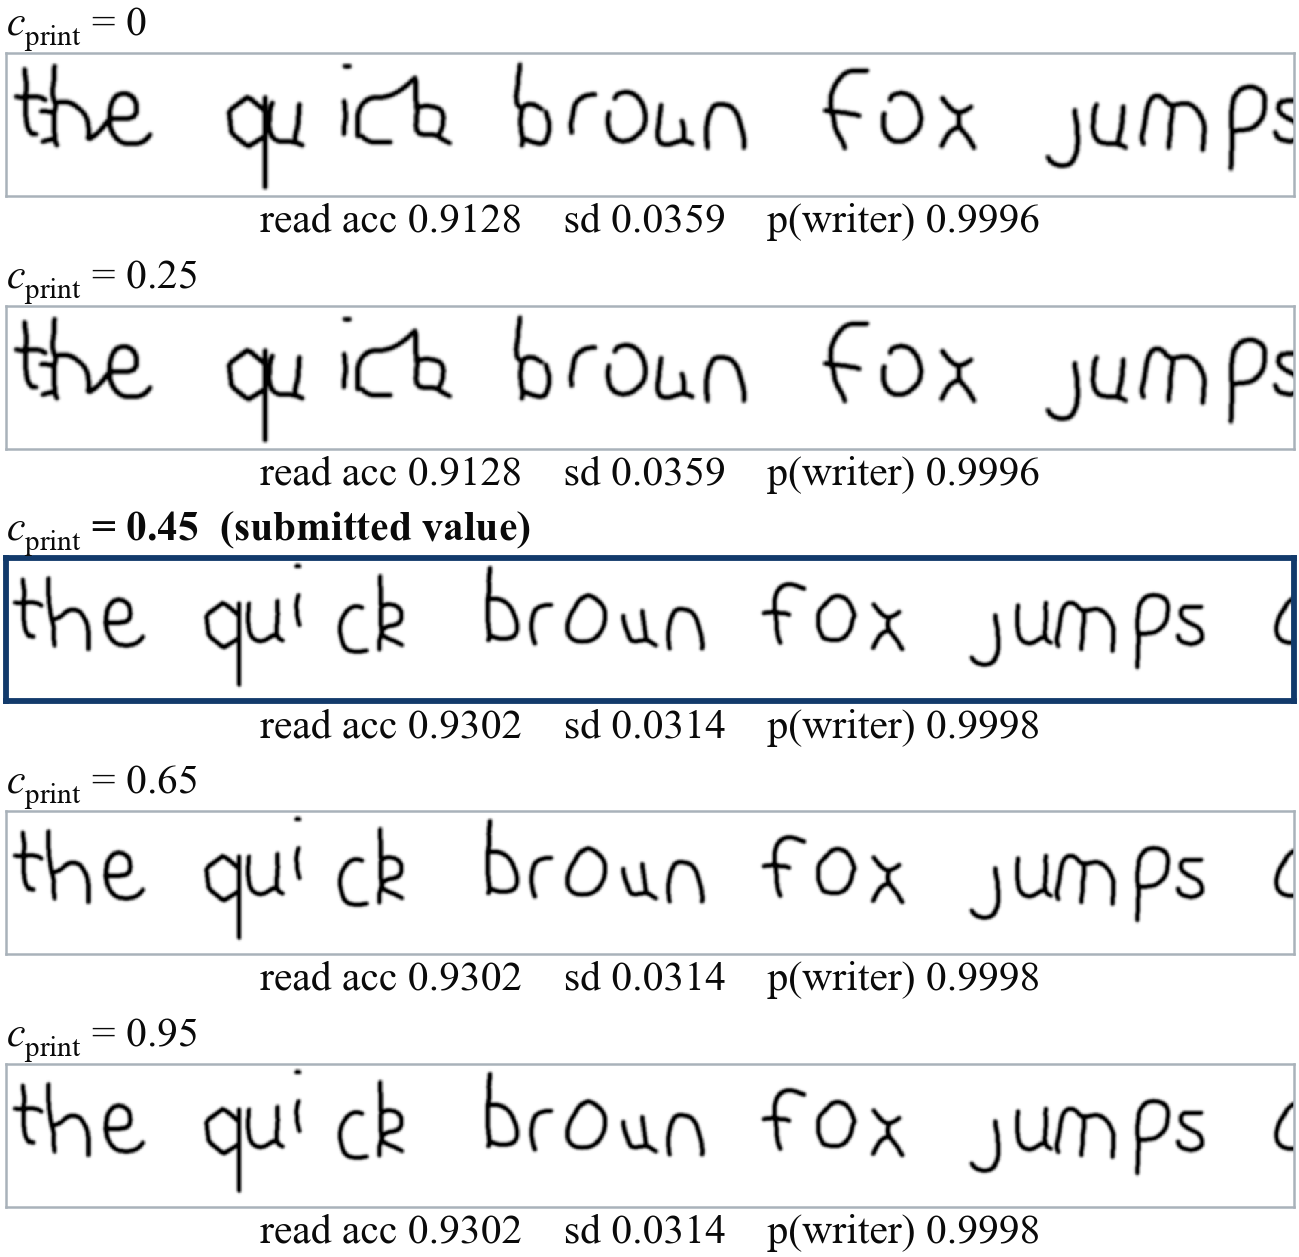
\includegraphics[width=\linewidth]{../figures/join_conn_floor.png}

\caption{Joinedness below which a hand is drawn as print and makes no joins. Each panel is the same input processed by the submitted code with only $c_{\text{print}}$ changed; the panel outlined in dark blue is the submitted value.}

\label{fig:join-conn-floor}

\end{figure}

\begin{figure}[htbp]

\centering

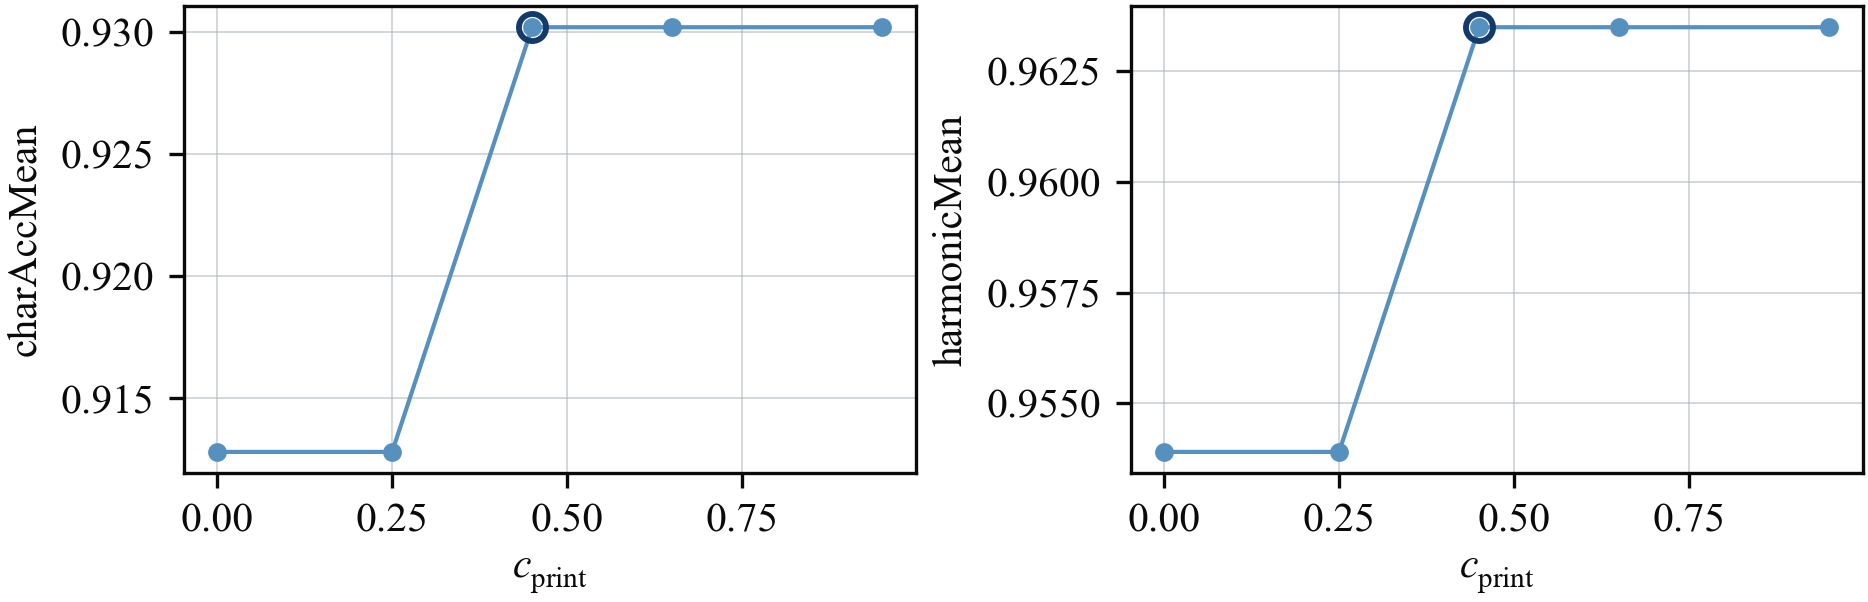
\includegraphics[width=\linewidth]{../figures/join_conn_floor_trend.png}

\caption{Joinedness below which a hand is drawn as print and makes no joins: measured quantities against the swept value. The circled point is the submitted value.}

\end{figure}

\begin{table}[htbp]
\centering
\small
\caption{Joinedness below which a hand is drawn as print and makes no joins: measured effect of each swept value. The submitted value is in bold.}
\begin{tabular}{lrrrrr}
\toprule
\$c\_\{\textbackslash\{\}text\{print\}\}\$ & \textsf{charAccMean} & \textsf{charAccSd} & \textsf{widConfMean} & \textsf{harmonicMean} & \textsf{nStrokes} \\
\midrule
0 & 0.9128 & 0.0359 & 0.9996 & 0.9539 & 59 \\
0.25 & 0.9128 & 0.0359 & 0.9996 & 0.9539 & 59 \\
\bfseries 0.45 & \bfseries 0.9302 & \bfseries 0.0314 & \bfseries 0.9998 & \bfseries 0.9635 & \bfseries 57 \\
0.65 & 0.9302 & 0.0314 & 0.9998 & 0.9635 & 57 \\
0.95 & 0.9302 & 0.0314 & 0.9998 & 0.9635 & 57 \\
\bottomrule
\end{tabular}
\end{table}

\subsection{Furthest apart two letters may be and still be joined}

\label{coef:max-join-gap}

\begin{description}[leftmargin=5.2em,style=sameline]

\item[Symbol] $g_{\text{join}}$

\item[Value] \texttt{0.8}

\item[Source] \texttt{synthesise.py}, \texttt{MAX\_JOIN\_GAP\_XH}

\item[Swept] \texttt{0.2}, \texttt{0.5}, \texttt{0.8}, \texttt{1.3}, \texttt{2.5}

\end{description}

\paragraph{Basis}

A ligature is a pen movement between two letters; its length is bounded by the letter spacing of the hand \cite{plamondon2000}.

\paragraph{Why this value}

A join is only drawn if the next letter starts within $g_{\text{join}}$ x-heights of where the pen left the last one. Beyond that the connecting stroke is longer than a letter and reads as a line through the word rather than a ligature. Letter gaps in these profiles are held between $0.03$ and $0.30$ x-heights, so $0.80$ allows a join across an ordinary gap with margin, and refuses one where a collision push or an unusually wide glyph has opened a real space.

\paragraph{What the coefficient does}

The gap is measured from the previous exit point to the start of the body stroke of the next letter, after the collision push, so it reflects where the ink actually is rather than the nominal advance. The test sits in a conjunction: both letters must be alphabetic, from compatible sources, and the random draw against \texttt{connEff} must succeed.

\paragraph{Alternatives considered}

Scaling the limit by the measured word gap of the writer, which would make it writer-specific at the cost of another measured quantity in the chain.

\paragraph{Worked example}

At $4$ mm per x-height a join is refused once the gap exceeds $0.8 \times 4 = 3.2$ mm.

\paragraph{What the sweep actually showed}

\textbf{Nothing distinguishable}, as anticipated: Owen is below the print floor at the submitted settings, so no joins are drawn and the gap limit has nothing to act on. The small positive differences at every value (paired $t$ between $+0.52$ and $+1.74$) are seed noise. Exercising this coefficient needs a writer whose connectedness is above $0.45$, and none of the five photographed writers in this probe set is.

\paragraph{Limits of this test}

Owen is below the print floor, so no joins are drawn at the submitted settings and this sweep is expected to show little or no change for this writer. That is itself the finding, and it is reported rather than hidden; the trend shows the stroke count unmoved.

\begin{figure}[htbp]

\centering

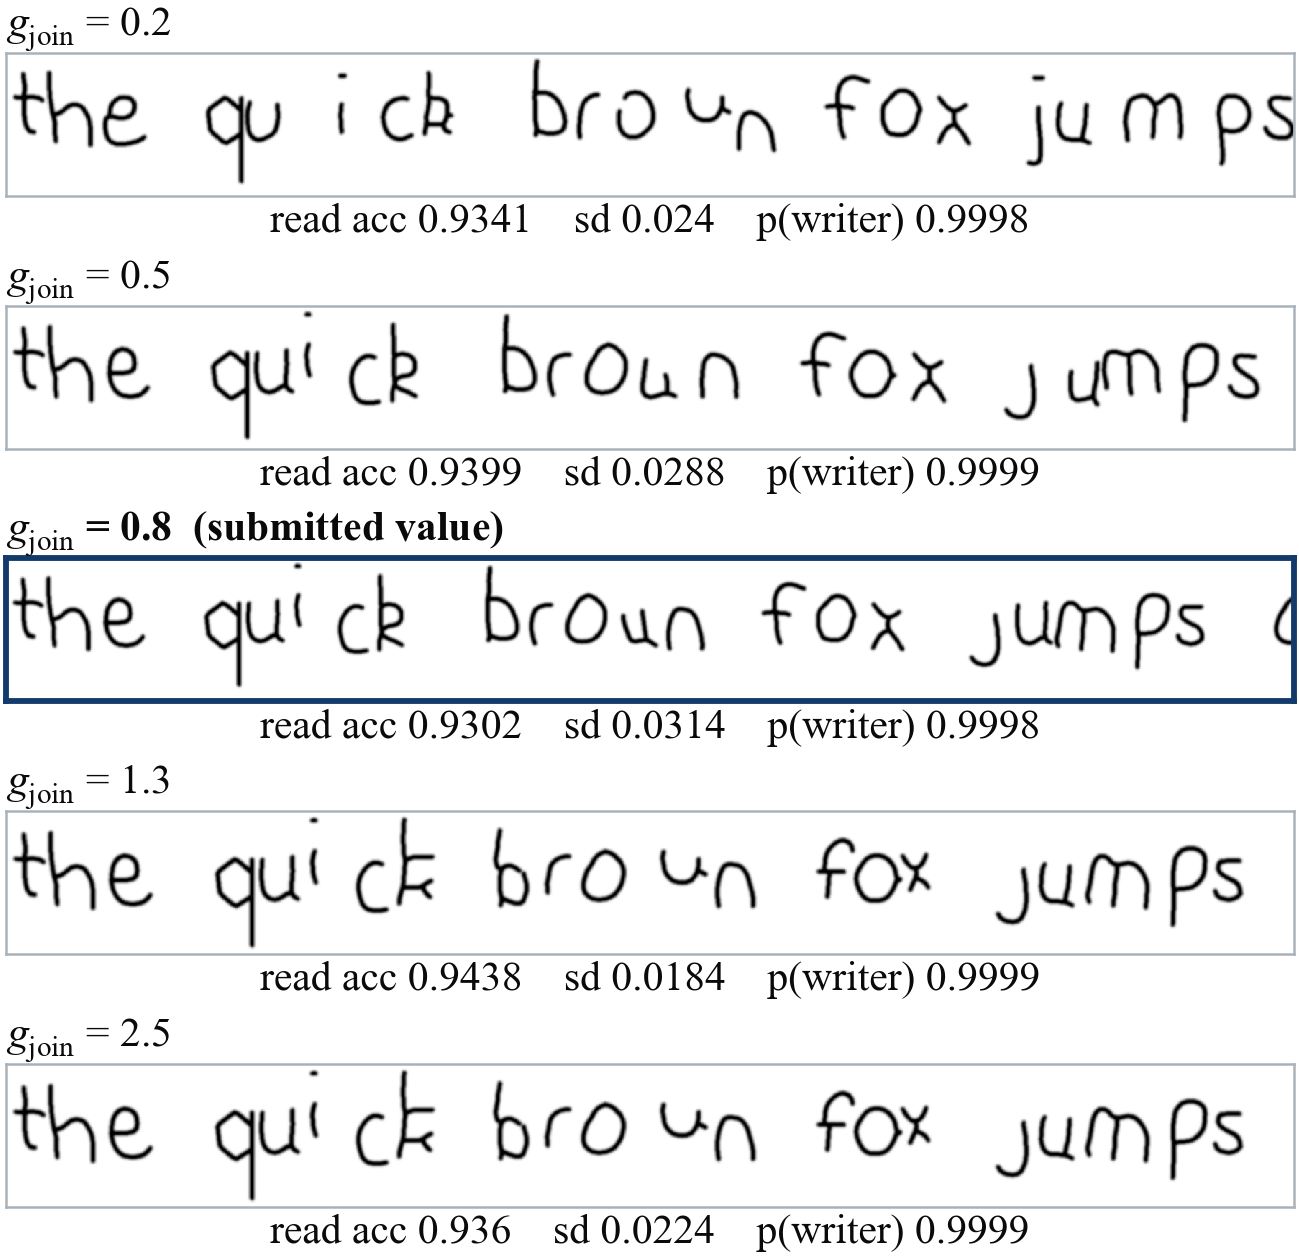
\includegraphics[width=\linewidth]{../figures/max_join_gap.png}

\caption{Furthest apart two letters may be and still be joined. Each panel is the same input processed by the submitted code with only $g_{\text{join}}$ changed; the panel outlined in dark blue is the submitted value.}

\label{fig:max-join-gap}

\end{figure}

\begin{figure}[htbp]

\centering

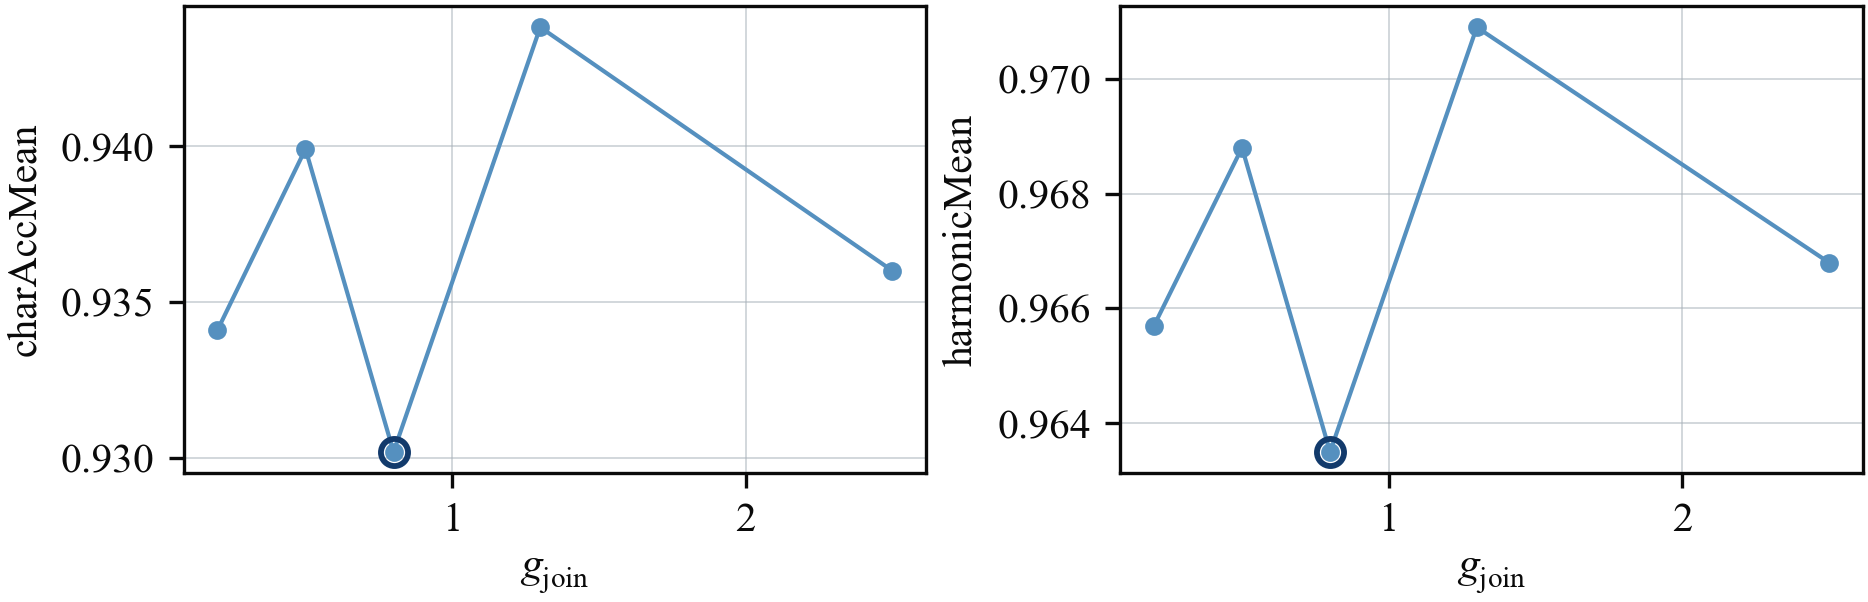
\includegraphics[width=\linewidth]{../figures/max_join_gap_trend.png}

\caption{Furthest apart two letters may be and still be joined: measured quantities against the swept value. The circled point is the submitted value.}

\end{figure}

\begin{table}[htbp]
\centering
\small
\caption{Furthest apart two letters may be and still be joined: measured effect of each swept value. The submitted value is in bold.}
\begin{tabular}{lrrrrr}
\toprule
\$g\_\{\textbackslash\{\}text\{join\}\}\$ & \textsf{charAccMean} & \textsf{charAccSd} & \textsf{widConfMean} & \textsf{harmonicMean} & \textsf{nStrokes} \\
\midrule
0.2 & 0.9341 & 0.024 & 0.9998 & 0.9657 & 59 \\
0.5 & 0.9399 & 0.0288 & 0.9999 & 0.9688 & 58 \\
\bfseries 0.8 & \bfseries 0.9302 & \bfseries 0.0314 & \bfseries 0.9998 & \bfseries 0.9635 & \bfseries 57 \\
1.3 & 0.9438 & 0.0184 & 0.9999 & 0.9709 & 60 \\
2.5 & 0.936 & 0.0224 & 0.9999 & 0.9668 & 60 \\
\bottomrule
\end{tabular}
\end{table}

\section{Synthesis: spacing}

\subsection{Clearance kept between one letter's ink and the next}

\label{coef:collision-gap}

\begin{description}[leftmargin=5.2em,style=sameline]

\item[Symbol] $d_{\text{clear}}$

\item[Value] \texttt{0.05}

\item[Source] \texttt{synthesise.py}, \texttt{COLLISION\_MIN\_GAP\_XH}

\item[Swept] \texttt{-0.1}, \texttt{0.0}, \texttt{0.05}, \texttt{0.2}, \texttt{0.5}

\end{description}

\paragraph{Basis}

Overlap resolution between adjacent glyphs is the layout problem solved by kerning in typography; in handwriting the equivalent constraint is that the pen does not retrace the previous letter \cite{plamondon2000}.

\paragraph{Why this value}

Each letter is placed by advancing the pen by the previous letter's advance, which is a measured number and takes no account of the particular shapes drawn. Two wide variants in a row can therefore overlap. The rule compares the right-most ink of the previous body stroke with the left-most ink of the new letter and pushes the new letter right if they are closer than $d_{\text{clear}}$. The value is small on purpose: the aim is to stop ink touching, not to impose uniform spacing, because uniform spacing is precisely what makes synthetic writing look printed. $0.05$ x-heights is about two pixels at the rendering scale, just enough to keep strokes apart.

\paragraph{What the coefficient does}

A negative value lets letters overlap, which the sweep includes to show what the rule is preventing. A large value forces every letter clear of the last and so overrides the writer's own measured advances, producing evenly spaced, mechanical output and a longer line.

\paragraph{Alternatives considered}

Testing true ink overlap by rasterising each pair, which is exact but far more expensive; or adjusting the advance rather than pushing, which changes the writer's measured rhythm.

\paragraph{Worked example}

At $4$ mm per x-height the clearance is $0.2$ mm, against a pen width of $0.085 \times 4 = 0.34$ mm, so adjacent strokes are kept about half a pen width apart.

\paragraph{What the sweep actually showed}

A significant result at the top of the range, in the \emph{opposite} direction to the design argument. At $d_{\text{clear}} = 0.5$ x-heights the paired gain over the submitted $0.05$ is $+0.0232$ reading accuracy ($6$ better, $0$ worse, $t = +2.87$) and $+0.0123$ on the joint score ($t = +2.81$). That is forcing a tenth of an x-height of clear space between every pair of letters, which spreads the writing out and makes it easier to read --- and the writer classifier does not object enough to cancel it. The argument against adopting it is the one given above and is not measured by either judge: uniform enforced spacing is what makes synthetic handwriting look mechanical, and neither the reader nor the writer classifier is sensitive to that. This is a case where the system's own metrics point one way and the design intent points the other, and the submitted value follows the intent. It should be defended on those grounds, not by claiming the metrics support it.

\begin{figure}[htbp]

\centering

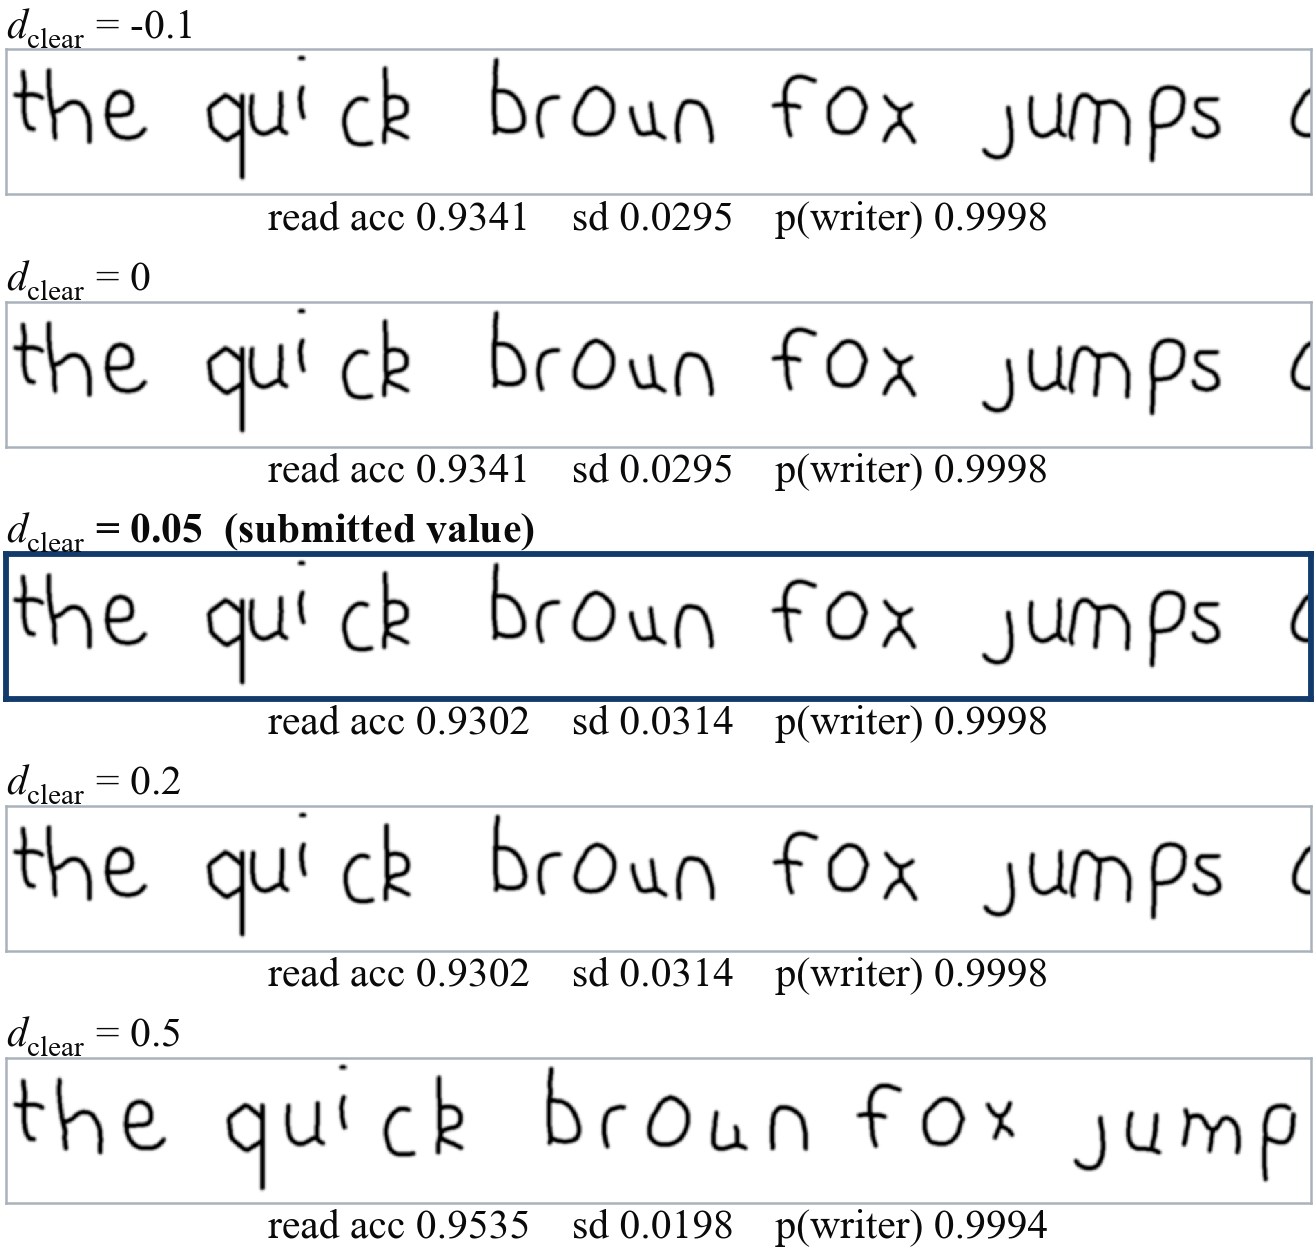
\includegraphics[width=\linewidth]{../figures/collision_gap.png}

\caption{Clearance kept between one letter's ink and the next. Each panel is the same input processed by the submitted code with only $d_{\text{clear}}$ changed; the panel outlined in dark blue is the submitted value.}

\label{fig:collision-gap}

\end{figure}

\begin{figure}[htbp]

\centering

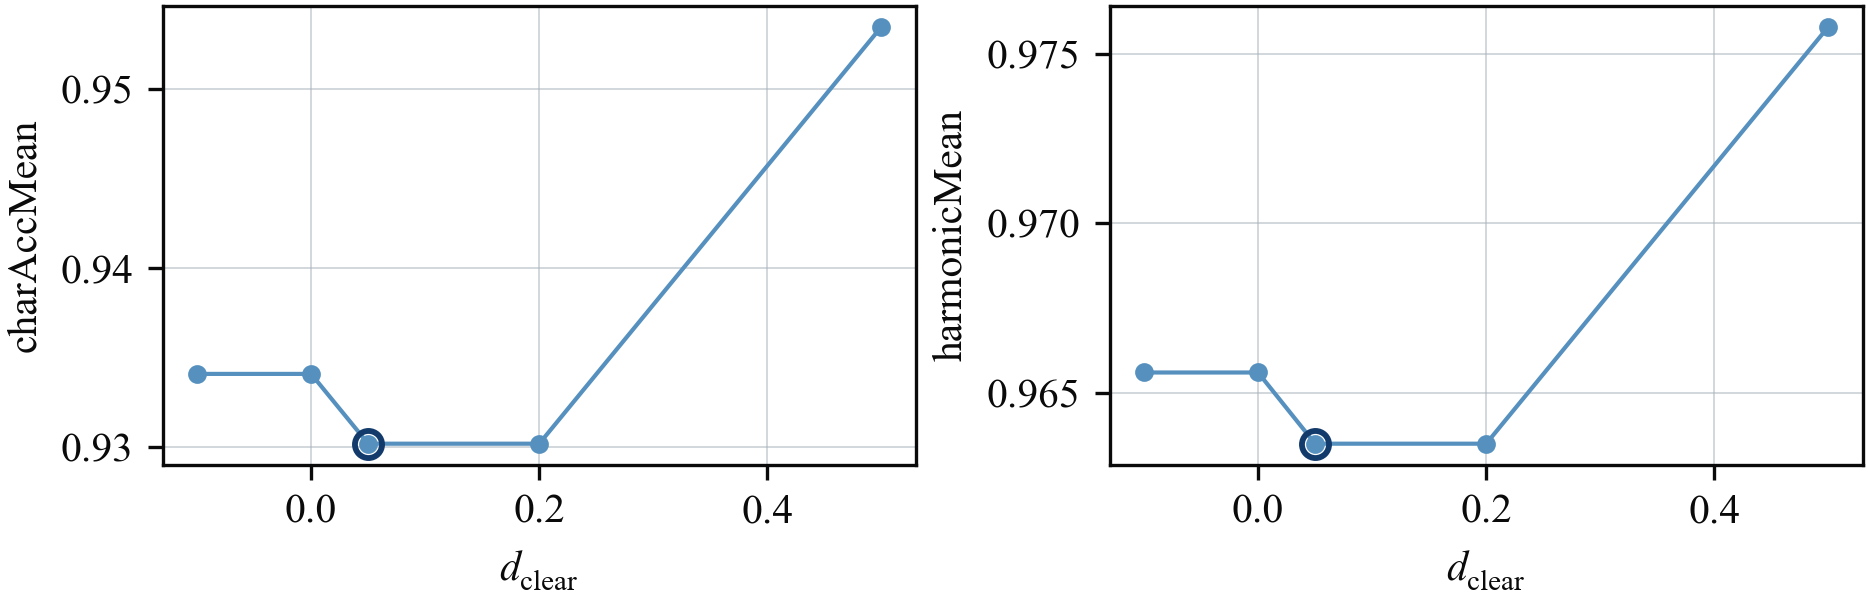
\includegraphics[width=\linewidth]{../figures/collision_gap_trend.png}

\caption{Clearance kept between one letter's ink and the next: measured quantities against the swept value. The circled point is the submitted value.}

\end{figure}

\begin{table}[htbp]
\centering
\small
\caption{Clearance kept between one letter's ink and the next: measured effect of each swept value. The submitted value is in bold.}
\begin{tabular}{lrrrr}
\toprule
\$d\_\{\textbackslash\{\}text\{clear\}\}\$ & \textsf{charAccMean} & \textsf{charAccSd} & \textsf{widConfMean} & \textsf{harmonicMean} \\
\midrule
-0.1 & 0.9341 & 0.0295 & 0.9998 & 0.9656 \\
0 & 0.9341 & 0.0295 & 0.9998 & 0.9656 \\
\bfseries 0.05 & \bfseries 0.9302 & \bfseries 0.0314 & \bfseries 0.9998 & \bfseries 0.9635 \\
0.2 & 0.9302 & 0.0314 & 0.9998 & 0.9635 \\
0.5 & 0.9535 & 0.0198 & 0.9994 & 0.9758 \\
\bottomrule
\end{tabular}
\end{table}

\section{Synthesis: variation}

\subsection{Persistence of the slow baseline drift}

\label{coef:drift-persistence}

\begin{description}[leftmargin=5.2em,style=sameline]

\item[Symbol] $\phi_{\text{drift}}$

\item[Value] \texttt{0.85}

\item[Source] \texttt{synthesise.py}, \texttt{SynthesizeText}

\item[Swept] \texttt{0.0}, \texttt{0.5}, \texttt{0.85}, \texttt{0.97}, \texttt{1.0}

\end{description}

\paragraph{Basis}

Handwriting is not produced on a perfectly straight baseline; slow drift is part of the motor variability of the writing process \cite{plamondon2000}, and baseline undulation is used as a writer-identification feature \cite{bulacu2007}.

\paragraph{Why this value}

Independent random offsets per letter give jitter, not drift: the baseline then looks noisy rather than wandering, because each letter is unrelated to its neighbour. Drift is modelled instead as a first-order autoregression, where a velocity $v$ is updated as $v \leftarrow \phi v + \mathcal{N}(0,\sigma)$ and accumulated into the offset. $\phi$ is the memory: it sets how many letters a drift persists for. At $0.85$ the correlation decays by half in $\ln 2/\ln(1/0.85) = 4.3$ letters, so a drift lasts about a word, which is the scale at which real baselines wander.

\paragraph{What the coefficient does}

At $\phi = 0$ the velocity is white noise and the baseline jitters per letter. At $\phi = 1$ the velocity is a random walk that never returns, so the line runs away downwards or upwards until the clip at $\pm 0.25$ x-heights catches it; that clip is what makes $\phi = 1$ survivable at all and is swept separately.

\paragraph{Alternatives considered}

A low-pass-filtered noise field, which is the same thing in the frequency domain, or a sinusoidal baseline, which is too regular to pass as handwriting.

\paragraph{Worked example}

With $\phi = 0.85$ the stationary standard deviation of the velocity is $\sigma/\sqrt{1-\phi^2} = 1.90\sigma$, where $\sigma = 0.35 \times 0.05 \times \text{jitter}$ x-heights.

\paragraph{What the sweep actually showed}

\textbf{No distinguishable effect} at any value, including $\phi = 0$ (white-noise jitter) and $\phi = 1$ (an unbounded random walk): nine to twelve of the twelve seeds are identical in every comparison and no paired $t$ exceeds $+1.0$. At the jitter setting used here the drift amplitude is $0.05 \times 0.15 = 0.0075$ x-heights per step with a further $0.35$ factor on the velocity, which is far too small to move a letter by a pixel at the rendering scale. So the autoregressive drift model is present but is contributing almost nothing at the default jitter, and the distinction between drift and jitter that motivates $\phi$ is not visible in the output. It would need a much larger jitter setting to be seen, and the figure at this setting should not be presented as showing baseline wander.

\begin{figure}[htbp]

\centering

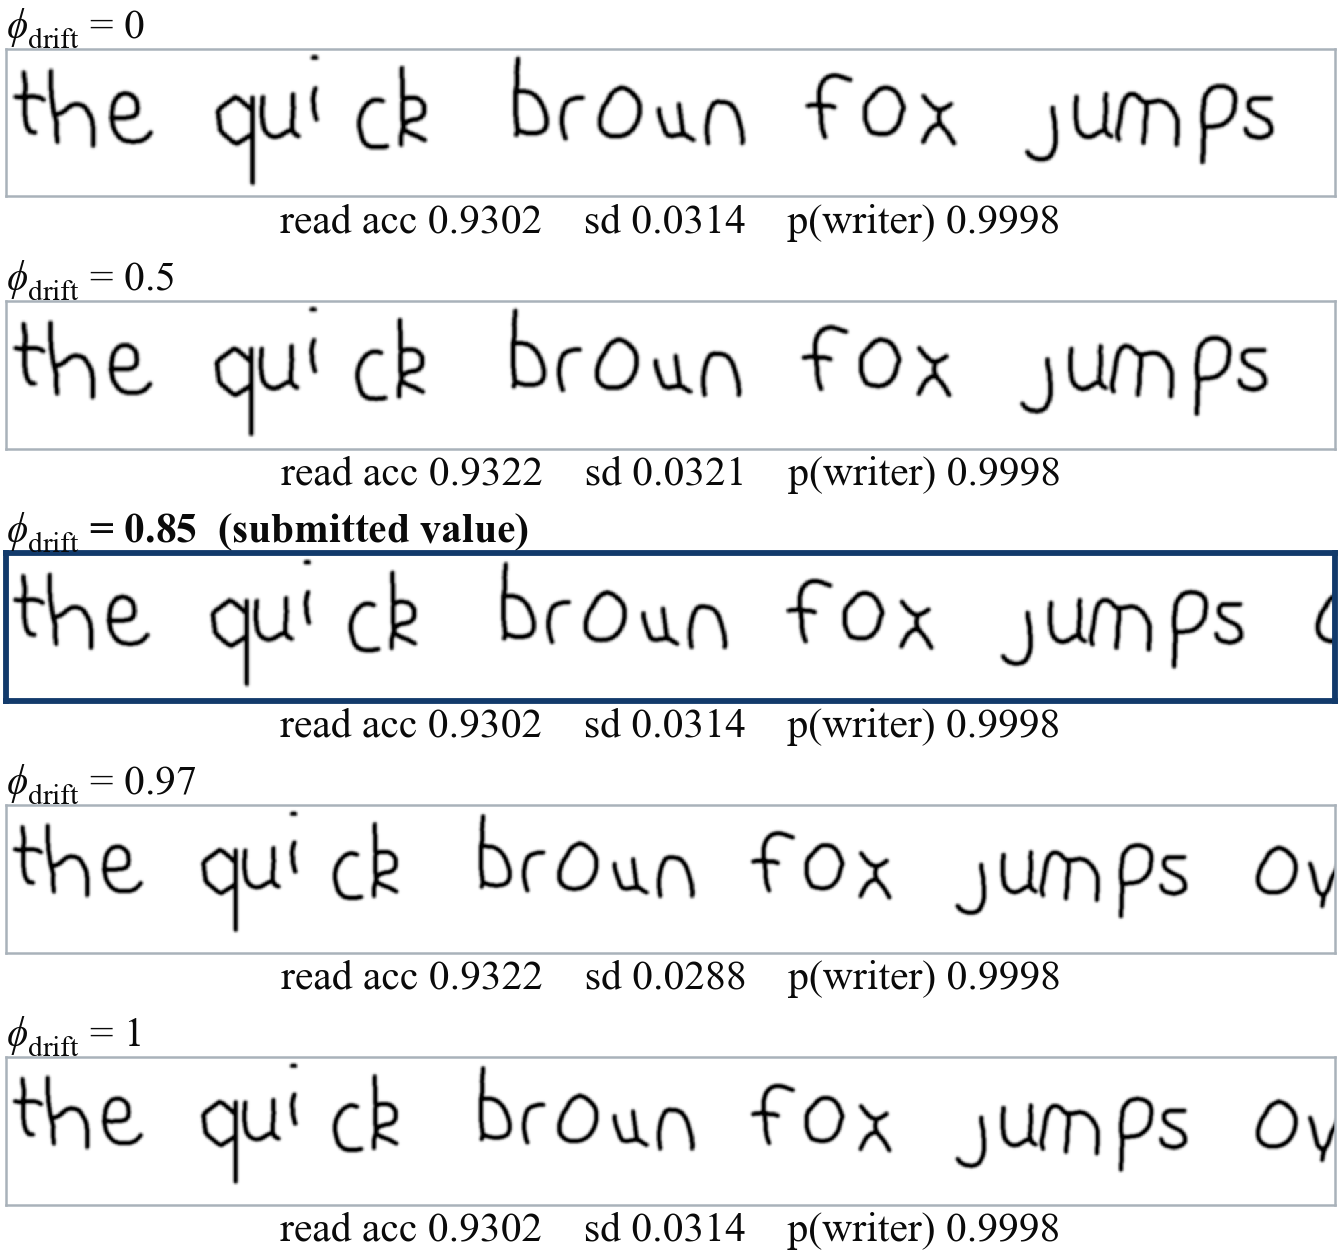
\includegraphics[width=\linewidth]{../figures/drift_persistence.png}

\caption{Persistence of the slow baseline drift. Each panel is the same input processed by the submitted code with only $\phi_{\text{drift}}$ changed; the panel outlined in dark blue is the submitted value.}

\label{fig:drift-persistence}

\end{figure}

\begin{figure}[htbp]

\centering

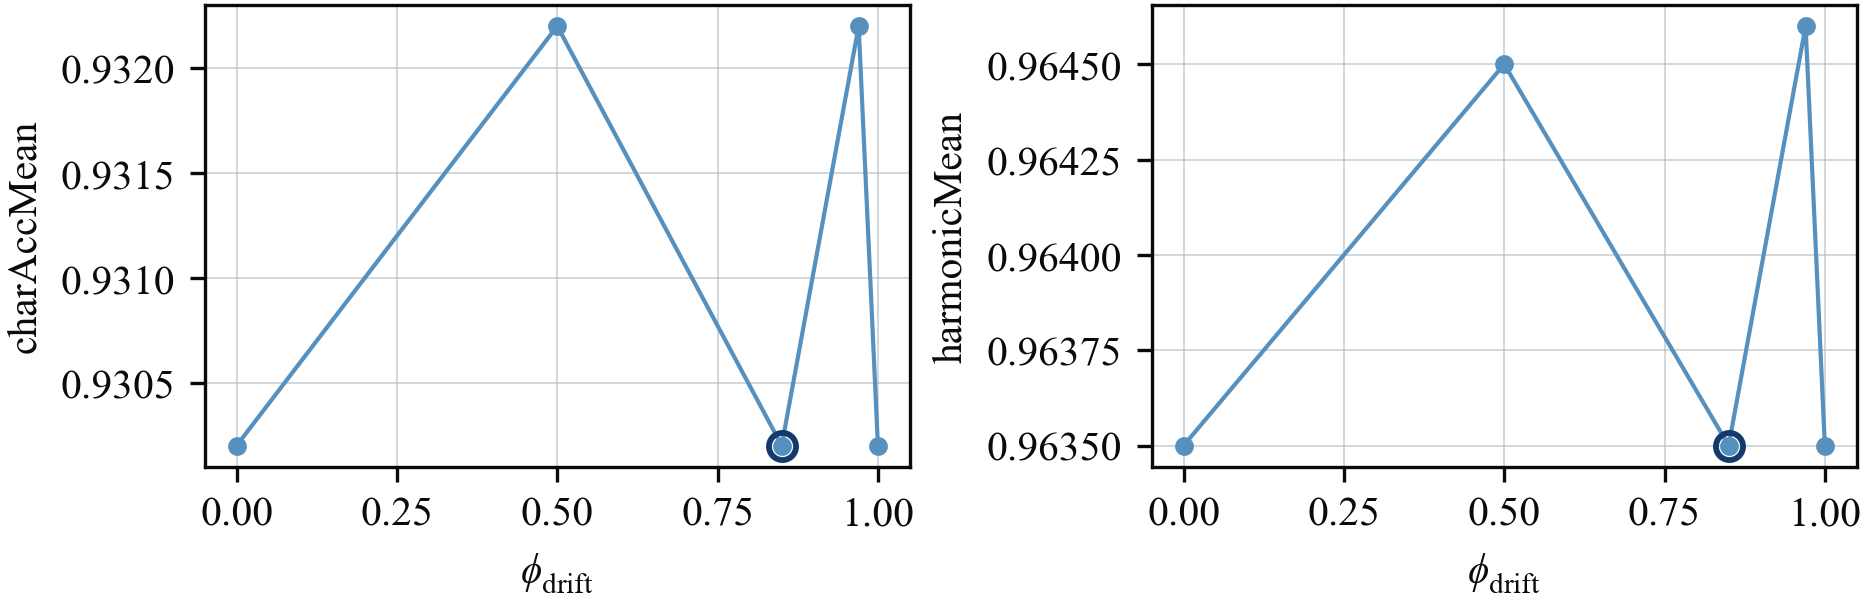
\includegraphics[width=\linewidth]{../figures/drift_persistence_trend.png}

\caption{Persistence of the slow baseline drift: measured quantities against the swept value. The circled point is the submitted value.}

\end{figure}

\begin{table}[htbp]
\centering
\small
\caption{Persistence of the slow baseline drift: measured effect of each swept value. The submitted value is in bold.}
\begin{tabular}{lrrrr}
\toprule
\$\textbackslash\{\}phi\_\{\textbackslash\{\}text\{drift\}\}\$ & \textsf{charAccMean} & \textsf{charAccSd} & \textsf{widConfMean} & \textsf{harmonicMean} \\
\midrule
0 & 0.9302 & 0.0314 & 0.9998 & 0.9635 \\
0.5 & 0.9322 & 0.0321 & 0.9998 & 0.9645 \\
\bfseries 0.85 & \bfseries 0.9302 & \bfseries 0.0314 & \bfseries 0.9998 & \bfseries 0.9635 \\
0.97 & 0.9322 & 0.0288 & 0.9998 & 0.9646 \\
1 & 0.9302 & 0.0314 & 0.9998 & 0.9635 \\
\bottomrule
\end{tabular}
\end{table}

\subsection{Largest baseline drift allowed}

\label{coef:drift-clip}

\begin{description}[leftmargin=5.2em,style=sameline]

\item[Symbol] $d_{\max}$

\item[Value] \texttt{0.25}

\item[Source] \texttt{synthesise.py}, \texttt{SynthesizeText}

\item[Swept] \texttt{0.02}, \texttt{0.1}, \texttt{0.25}, \texttt{0.6}, \texttt{1.5}

\end{description}

\paragraph{Basis}

Bounding an accumulated random walk is necessary whenever the walk has no restoring force; the writing-line constraint itself is physical, since the writer sees and corrects the baseline \cite{plamondon2000}.

\paragraph{Why this value}

The drift velocity is autoregressive but the drift itself is a sum of those velocities, which is a random walk: over a long line it would wander arbitrarily far. Real writers correct against the ruling, so the model clips the accumulated drift. The limit is in x-heights and $0.25$ is a quarter of the body height, which is visible as a wavering baseline but never enough to let one line collide with the next, since lines are set $\text{asc}-\text{desc}+0.85$ x-heights apart.

\paragraph{What the coefficient does}

The clip is also what keeps $\phi$ near $1$ usable. It acts as a hard wall rather than a restoring force, so with a persistent velocity the drift can sit against the wall for many letters, which looks like a sloping line rather than a wandering one.

\paragraph{Alternatives considered}

An Ornstein--Uhlenbeck process on the drift itself, which pulls back towards zero smoothly instead of clipping and would be the better model; or re-centring at each word.

\paragraph{Worked example}

At $4$ mm per x-height the drift is bounded at $\pm 1.0$ mm, against a line pitch of $(1.51+0.68+0.85) \times 4 = 12.2$ mm for Owen.

\paragraph{What the sweep actually showed}

\textbf{No distinguishable effect}: eleven of twelve seeds identical at every value, and the one that moves gives a paired $t = +1.00$. At $4$ mm per x-height the clip is $\pm 1.0$ mm against a line step of $12.2$ mm, and the jitter setting used here ($0.15$) makes the drift velocity small enough that the accumulated drift rarely approaches the clip at all. The clip is a guard against a random walk running away over a long line, and a $43$-character sentence at low jitter does not run far enough to meet it.

\begin{figure}[htbp]

\centering

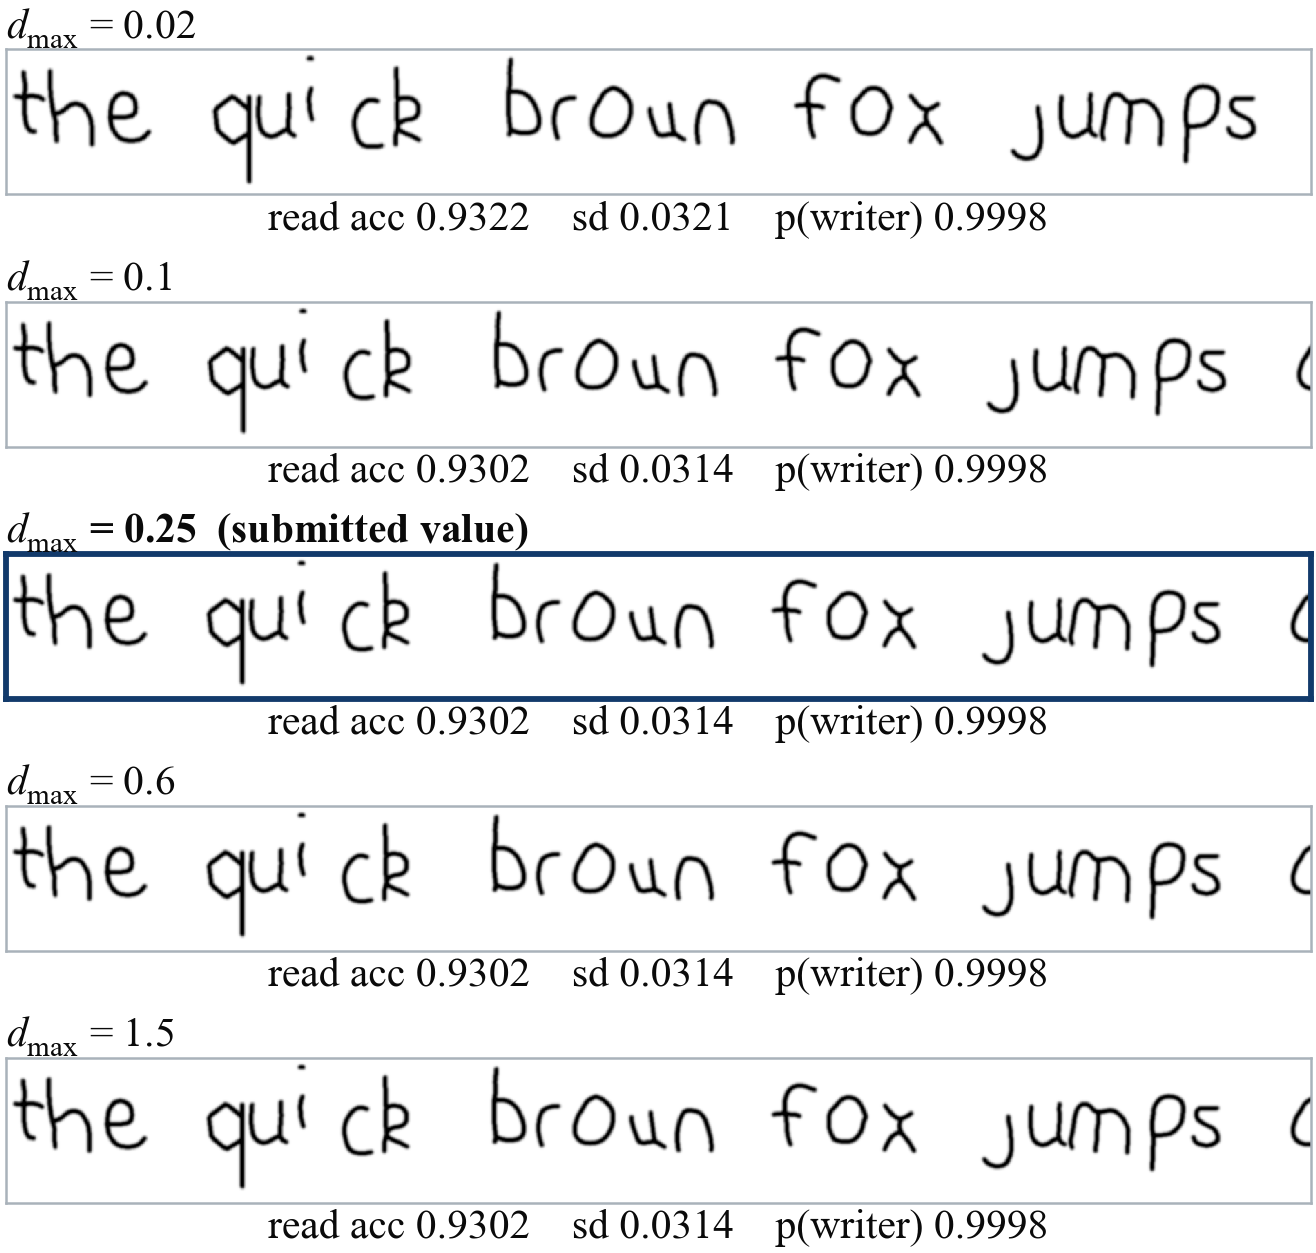
\includegraphics[width=\linewidth]{../figures/drift_clip.png}

\caption{Largest baseline drift allowed. Each panel is the same input processed by the submitted code with only $d_{\max}$ changed; the panel outlined in dark blue is the submitted value.}

\label{fig:drift-clip}

\end{figure}

\begin{figure}[htbp]

\centering

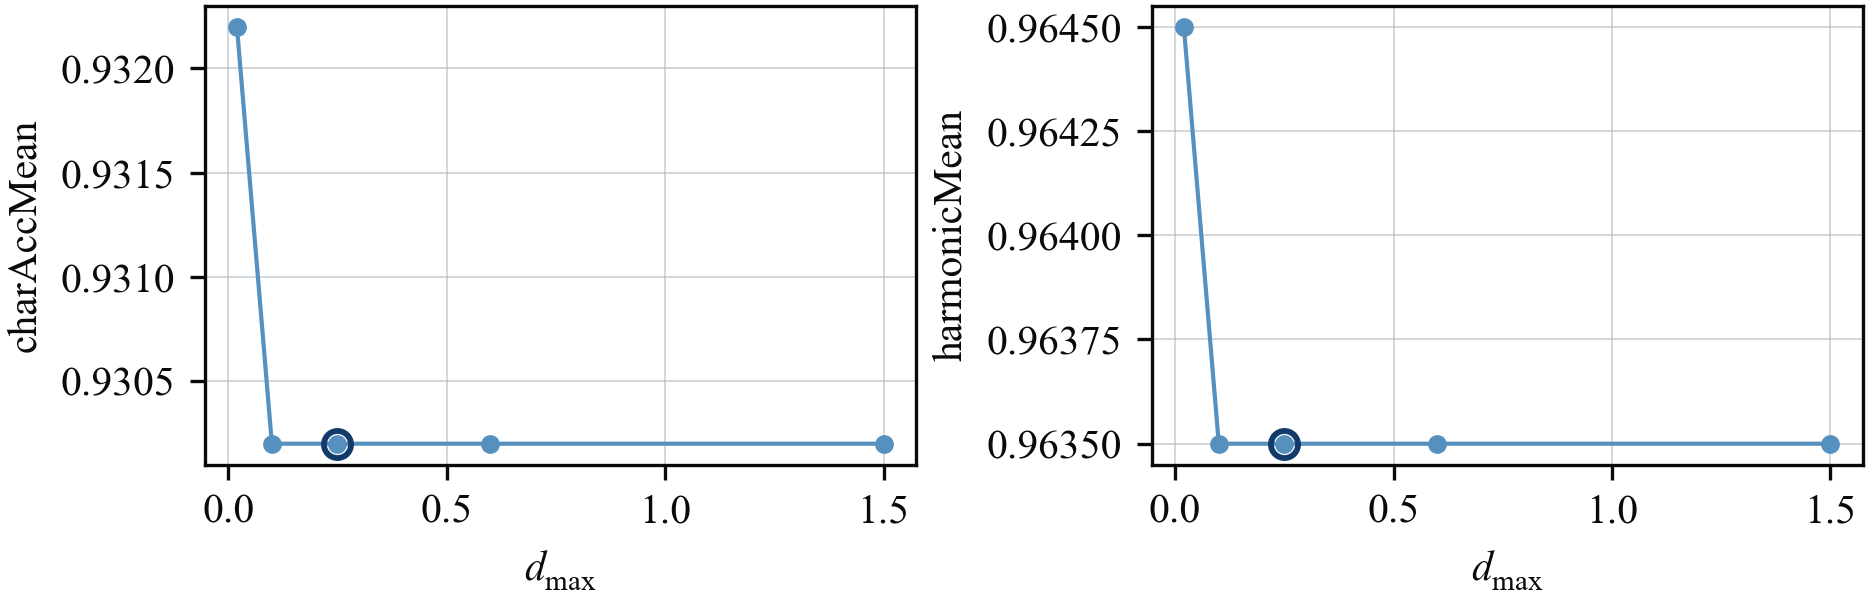
\includegraphics[width=\linewidth]{../figures/drift_clip_trend.png}

\caption{Largest baseline drift allowed: measured quantities against the swept value. The circled point is the submitted value.}

\end{figure}

\begin{table}[htbp]
\centering
\small
\caption{Largest baseline drift allowed: measured effect of each swept value. The submitted value is in bold.}
\begin{tabular}{lrrrr}
\toprule
\$d\_\{\textbackslash\{\}max\}\$ & \textsf{charAccMean} & \textsf{charAccSd} & \textsf{widConfMean} & \textsf{harmonicMean} \\
\midrule
0.02 & 0.9322 & 0.0321 & 0.9998 & 0.9645 \\
0.1 & 0.9302 & 0.0314 & 0.9998 & 0.9635 \\
\bfseries 0.25 & \bfseries 0.9302 & \bfseries 0.0314 & \bfseries 0.9998 & \bfseries 0.9635 \\
0.6 & 0.9302 & 0.0314 & 0.9998 & 0.9635 \\
1.5 & 0.9302 & 0.0314 & 0.9998 & 0.9635 \\
\bottomrule
\end{tabular}
\end{table}

\section{Synthesis: rendering}

\subsection{Pen width the synthesised line is rendered at}

\label{coef:uniform-pen-width}

\begin{description}[leftmargin=5.2em,style=sameline]

\item[Symbol] $w_{\text{draw}}$

\item[Value] \texttt{0.085}

\item[Source] \texttt{synthesise.py}, \texttt{UNIFORM\_PEN\_WIDTH\_XH}

\item[Swept] \texttt{0.03}, \texttt{0.055}, \texttt{0.085}, \texttt{0.14}, \texttt{0.22}

\end{description}

\paragraph{Basis}

Stroke width is a writer-discriminative property \cite{brink2012, bulacu2007}, which is why a single machine pen must be modelled explicitly rather than inherited from the source writer.

\paragraph{Why this value}

The rendered image exists to be judged by the same two networks that judge real pages, so it must look like what the machine will actually draw. The machine has one pen, so every writer is rendered at one width, and that width is the physical one: a $0.7$ mm ballpoint at $4$ mm per x-height is $0.7/4 = 0.175$ x-heights of \emph{diameter}, and the renderer takes $w_{\text{draw}}$ as a width in x-heights before the soft edge is added, which at $0.085$ plus a $30\%$ soft fringe lands close to that measured line. It is deliberately not the writer's own measured \texttt{strokeWidthXh}, because the machine cannot vary its pen.

\paragraph{What the coefficient does}

Rendering too thin makes the judges see a different kind of image from their training data, in which real ballpoint strokes are several pixels wide; too thick fills in the counters of \texttt{a}, \texttt{e} and \texttt{o}, and the reader's accuracy falls because the letters stop being distinguishable. The sweep measures both judges, so the two failure modes are visible separately.

\paragraph{Alternatives considered}

Rendering each writer at their own measured stroke width, which flatters the writer classifier but misrepresents the machine; or not rendering at all and scoring the trajectory geometrically, which cannot use the trained judges.

\paragraph{Worked example}

At $4$ mm per x-height and $18$ px/mm the pen is $0.085 \times 4 \times 18 = 6.1 \to 6$ px, blurred with $\sigma = 0.30 \times 6 = 1.8$ px.

\paragraph{What the sweep actually showed}

Over twelve seeds, \textbf{a thicker pen scores significantly better than the submitted one}. Against $0.085$, rendering at $0.14$ gives a paired mean gain of $+0.0155$ in reading accuracy ($6$ seeds better, $0$ worse, $6$ unchanged, paired $t = +2.97$) and $+0.0083$ on the joint text-and-writer score ($t = +2.96$), both past the two-sided $5\,\%$ point. Thinner ($0.03$) and much thicker ($0.22$) are not distinguishable from the submitted value. Two things must be said before this is read as \enquote{the value is wrong}. First, this coefficient does \textbf{not} change what the machine draws: the pen path and therefore the G-code are identical at every value, and only the rendered image used for scoring changes. So what the sweep has found is that the system's own judges prefer a slightly thicker rendering, which is a statement about the evaluation harness as much as about the writing. Second, the submitted value is tied to a physical quantity, the $0.7$ mm trace of the actual pen, and moving it to flatter the judges would make the preview less like what the robot really puts on paper. The finding is recorded; it is not a reason to change the value without first measuring the real drawn line.

\begin{figure}[htbp]

\centering

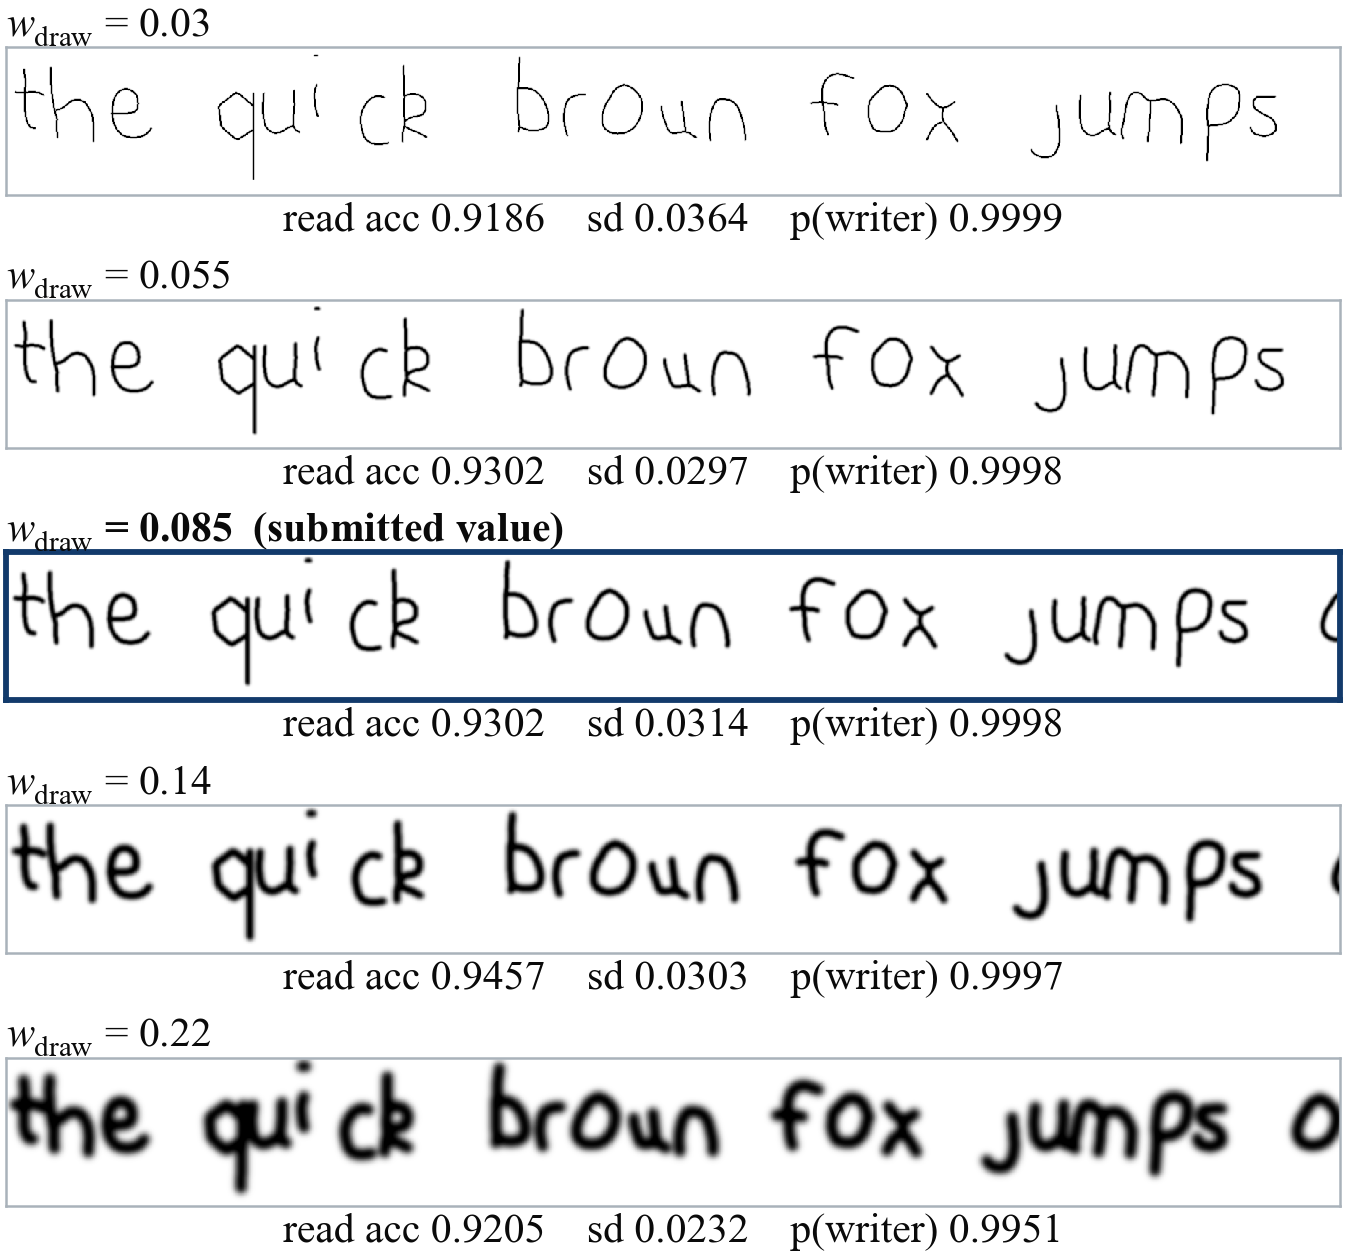
\includegraphics[width=\linewidth]{../figures/uniform_pen_width.png}

\caption{Pen width the synthesised line is rendered at. Each panel is the same input processed by the submitted code with only $w_{\text{draw}}$ changed; the panel outlined in dark blue is the submitted value.}

\label{fig:uniform-pen-width}

\end{figure}

\begin{figure}[htbp]

\centering

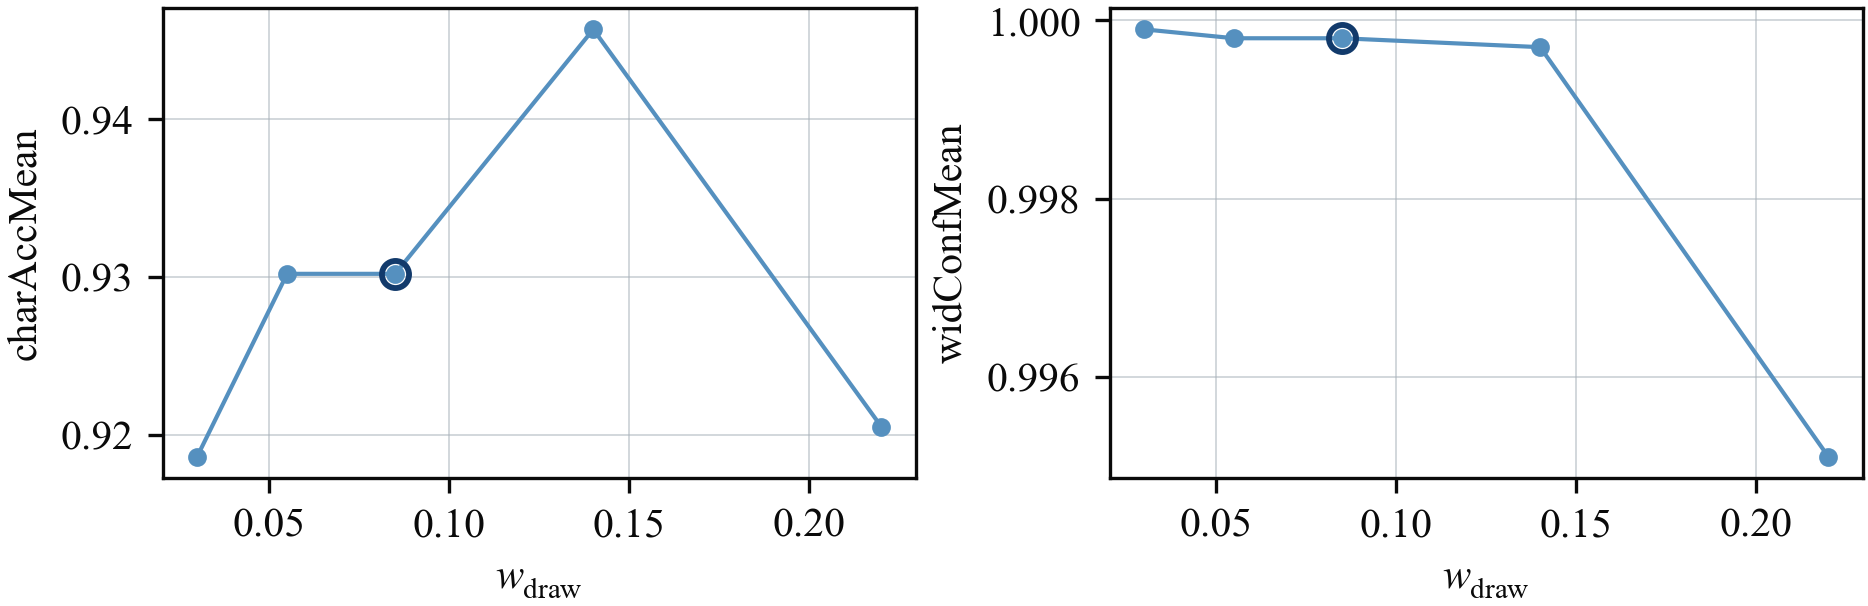
\includegraphics[width=\linewidth]{../figures/uniform_pen_width_trend.png}

\caption{Pen width the synthesised line is rendered at: measured quantities against the swept value. The circled point is the submitted value.}

\end{figure}

\begin{table}[htbp]
\centering
\small
\caption{Pen width the synthesised line is rendered at: measured effect of each swept value. The submitted value is in bold.}
\begin{tabular}{lrrrr}
\toprule
\$w\_\{\textbackslash\{\}text\{draw\}\}\$ & \textsf{charAccMean} & \textsf{charAccSd} & \textsf{widConfMean} & \textsf{harmonicMean} \\
\midrule
0.03 & 0.9186 & 0.0364 & 0.9999 & 0.9572 \\
0.055 & 0.9302 & 0.0297 & 0.9998 & 0.9635 \\
\bfseries 0.085 & \bfseries 0.9302 & \bfseries 0.0314 & \bfseries 0.9998 & \bfseries 0.9635 \\
0.14 & 0.9457 & 0.0303 & 0.9997 & 0.9717 \\
0.22 & 0.9205 & 0.0232 & 0.9951 & 0.9563 \\
\bottomrule
\end{tabular}
\end{table}

\subsection{Softness of the rendered stroke edge}

\label{coef:uniform-soft-frac}

\begin{description}[leftmargin=5.2em,style=sameline]

\item[Symbol] $s_{\text{soft}}$

\item[Value] \texttt{0.3}

\item[Source] \texttt{synthesise.py}, \texttt{UNIFORM\_SOFT\_FRAC}

\item[Swept] \texttt{0.0}, \texttt{0.15}, \texttt{0.3}, \texttt{0.6}, \texttt{1.0}

\end{description}

\paragraph{Basis}

A Gaussian point-spread is the standard first-order model of optical and sensor blur in an imaging chain \cite{itu601}; anti-aliasing a drawn edge is the equivalent in synthesis.

\paragraph{Why this value}

A polyline drawn with a hard round pen has a perfectly sharp edge, which no photograph of real ink has. The networks were trained on photographed crops whose stroke edges are soft, so a hard-edged render is out of distribution in a way that has nothing to do with the handwriting. The blur radius is tied to the pen width rather than fixed, so the softness scales with the writing. $0.30$ of the pen width is a little under half a stroke, enough to remove the staircase without visibly thickening the line.

\paragraph{What the coefficient does}

The blur is applied to the rendered image, so it also dims the stroke core slightly for a thin pen: at $s_{\text{soft}} = 1.0$ the Gaussian is as wide as the stroke and the ink no longer reaches full black, which changes the ink level the writer classifier sees.

\paragraph{Alternatives considered}

Supersampling the render and downsampling, which gives true area coverage instead of a blur, at several times the cost; or no softening at all.

\paragraph{Worked example}

At a $6$ px pen the blur is $\sigma = 1.8$ px, cut off at three sigma, so the kernel is $11$ px wide.

\paragraph{What the sweep actually showed}

The sweep contradicts the stated rationale at one end and confirms it strongly at the other. \textbf{No softening at all ($s_{\text{soft}} = 0$) scores significantly better} than the submitted $0.30$: a paired gain of $+0.0116$ in reading accuracy ($7$ better, $2$ worse, $t = +3.32$) and $+0.0062$ on the joint score ($t = +3.30$). At the other end, $s_{\text{soft}} = 1.0$ is much worse --- $-0.0465$ reading accuracy, and $12$ of $12$ seeds worse on the joint score, $t = -4.31$ --- which is the blur swallowing the stroke exactly as predicted. So the upper limit of the argument holds and the lower one does not: on this writer the networks do not need the soft edge that was meant to match their training distribution, and a hard-edged render reads slightly better. As with the pen width, this changes only the scored image and not the G-code. The honest position is that $0.30$ is defensible on the distribution-matching argument but is not the best value by the system's own measure, and the sweep says so.

\begin{figure}[htbp]

\centering

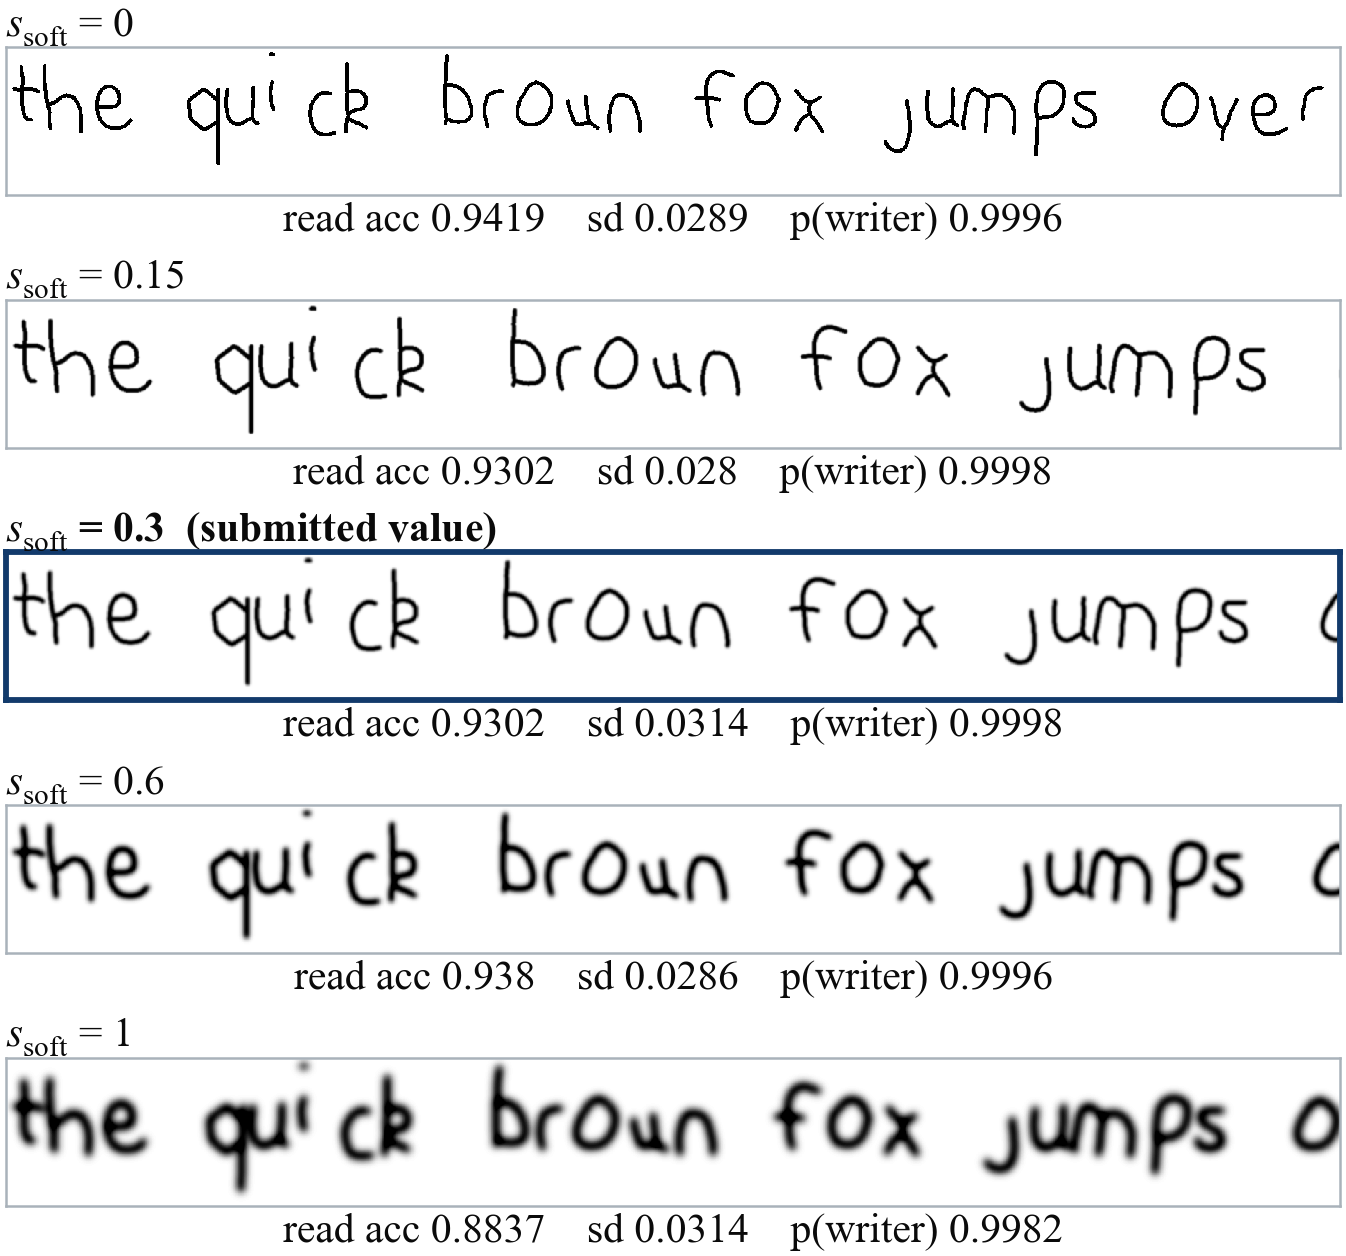
\includegraphics[width=\linewidth]{../figures/uniform_soft_frac.png}

\caption{Softness of the rendered stroke edge. Each panel is the same input processed by the submitted code with only $s_{\text{soft}}$ changed; the panel outlined in dark blue is the submitted value.}

\label{fig:uniform-soft-frac}

\end{figure}

\begin{figure}[htbp]

\centering

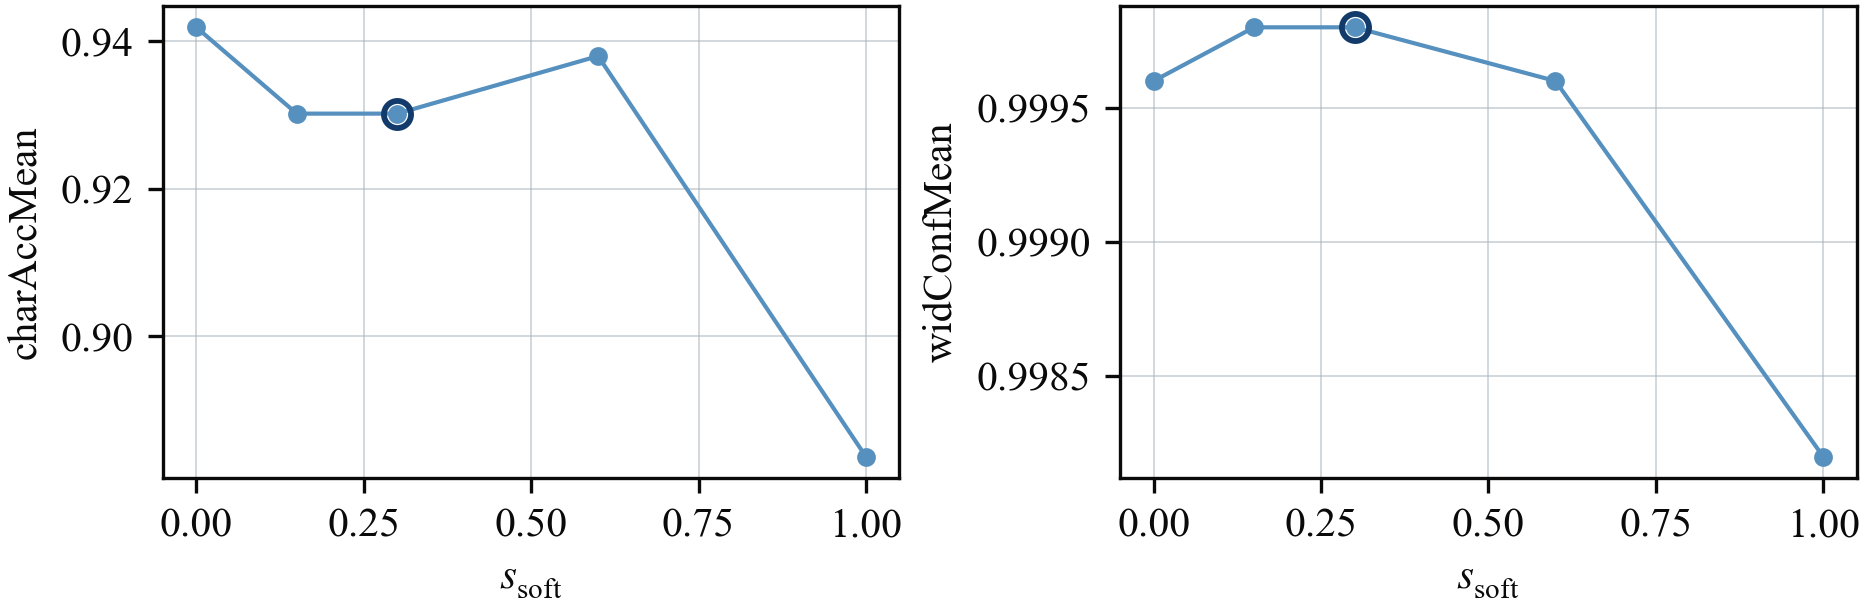
\includegraphics[width=\linewidth]{../figures/uniform_soft_frac_trend.png}

\caption{Softness of the rendered stroke edge: measured quantities against the swept value. The circled point is the submitted value.}

\end{figure}

\begin{table}[htbp]
\centering
\small
\caption{Softness of the rendered stroke edge: measured effect of each swept value. The submitted value is in bold.}
\begin{tabular}{lrrrr}
\toprule
\$s\_\{\textbackslash\{\}text\{soft\}\}\$ & \textsf{charAccMean} & \textsf{charAccSd} & \textsf{widConfMean} & \textsf{harmonicMean} \\
\midrule
0 & 0.9419 & 0.0289 & 0.9996 & 0.9697 \\
0.15 & 0.9302 & 0.028 & 0.9998 & 0.9636 \\
\bfseries 0.3 & \bfseries 0.9302 & \bfseries 0.0314 & \bfseries 0.9998 & \bfseries 0.9635 \\
0.6 & 0.938 & 0.0286 & 0.9996 & 0.9676 \\
1 & 0.8837 & 0.0314 & 0.9982 & 0.9372 \\
\bottomrule
\end{tabular}
\end{table}

\section{Synthesis: shape choice}

\subsection{How many of a letter's stored shapes may be drawn from}

\label{coef:eligible-variants}

\begin{description}[leftmargin=5.2em,style=sameline]

\item[Symbol] $V_{\text{elig}}$

\item[Value] \texttt{5}

\item[Source] \texttt{synthesise.py}, \texttt{\_ELIGIBLE\_VARIANTS}

\item[Swept] \texttt{1}, \texttt{2}, \texttt{5}, \texttt{10}, \texttt{20}

\end{description}

\paragraph{Basis}

A writer draws on a repertoire of allographs per letter rather than one fixed form \cite{schomaker1990}; repetition of an identical form is a signature of machine rather than human production \cite{plamondon2000}.

\paragraph{Why this value}

The stored variants are ranked by how typical they are, and only the top $V_{\text{elig}}$ are eligible, with weight $1/(1+1.4i)$ falling down the ranking. The limit exists because the tail of the ranking is where the badly cut glyphs are: a store of twelve variants may hold three or four that are fragments. Drawing from five keeps visible variety while staying in the part of the ranking that has been filtered twice, by the letter prior and by this writer's own consensus.

\paragraph{What the coefficient does}

At $V_{\text{elig}} = 1$ the most typical shape is drawn every time, so every instance of a letter is identical and the output looks like a font built from the writer's hand. Raising it reaches further into the ranking; because the weights fall as $1/(1+1.4i)$, variant $10$ is drawn with weight $0.067$ against $1.0$ for the first, so the effect saturates.

\paragraph{Alternatives considered}

Uniform sampling over all variants, which draws fragments as often as good shapes; or sampling weighted by the prior distance directly rather than by rank.

\paragraph{Worked example}

The weights for the first five ranks are $1,\,0.417,\,0.263,\,0.192,\,0.152$, summing to $2.02$, so the most typical shape is drawn about half the time.

\paragraph{What the sweep actually showed}

\textbf{Nothing is distinguishable from the submitted value} once twelve seeds are used. The paired differences against $V_{\text{elig}} = 5$ are $+0.0044$ at $1$, $+0.0012$ at $2$, $-0.0021$ at $10$ and $-0.0001$ at $20$ on the joint score, with paired $t$ between $-0.32$ and $+1.22$, all far inside the noise. This corrects what a single seed suggested, where $2$ appeared better and $10$ appeared worse by a clear margin; both were seed effects. The sweep therefore supports the design argument --- the ranking weights make the choice saturate --- and gives no evidence for moving the value either way.

\begin{figure}[htbp]

\centering

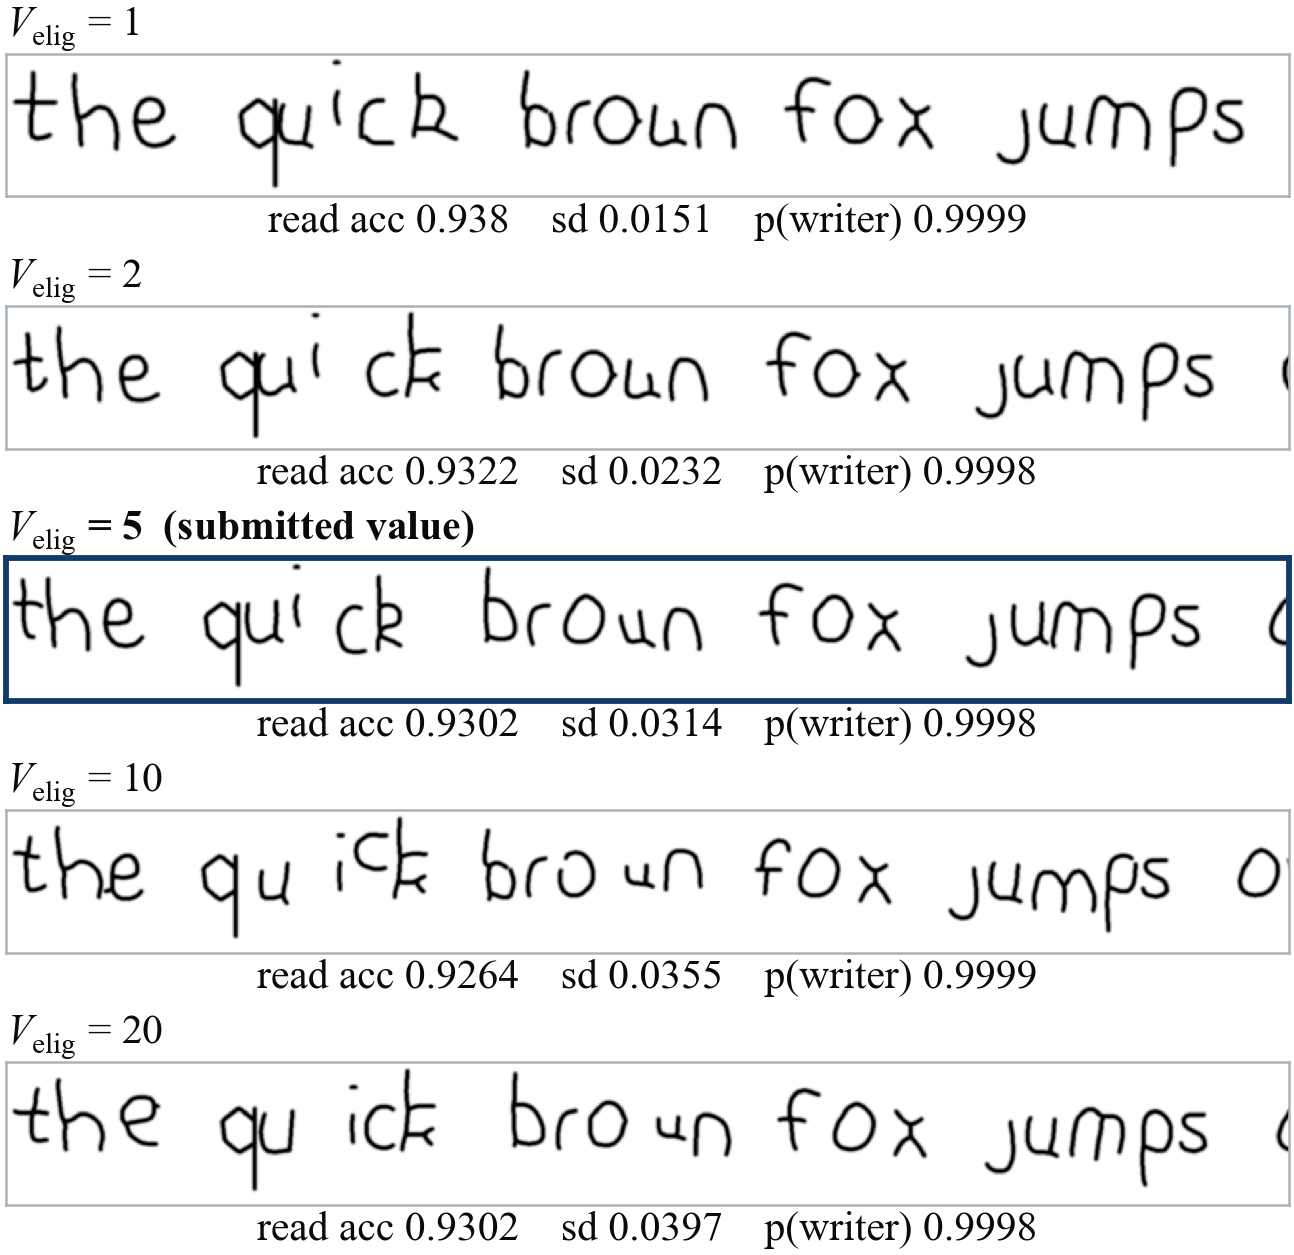
\includegraphics[width=\linewidth]{../figures/eligible_variants.png}

\caption{How many of a letter's stored shapes may be drawn from. Each panel is the same input processed by the submitted code with only $V_{\text{elig}}$ changed; the panel outlined in dark blue is the submitted value.}

\label{fig:eligible-variants}

\end{figure}

\begin{figure}[htbp]

\centering

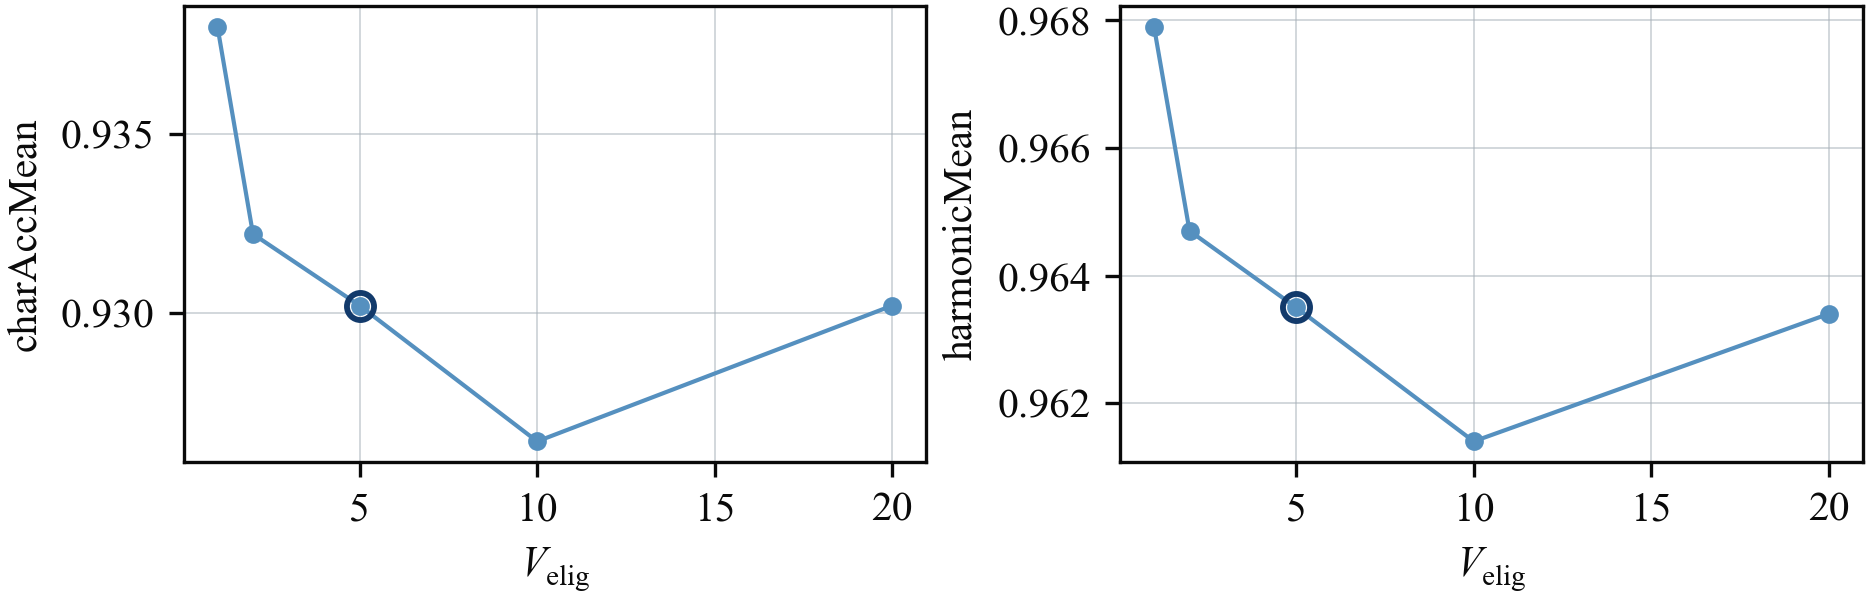
\includegraphics[width=\linewidth]{../figures/eligible_variants_trend.png}

\caption{How many of a letter's stored shapes may be drawn from: measured quantities against the swept value. The circled point is the submitted value.}

\end{figure}

\begin{table}[htbp]
\centering
\small
\caption{How many of a letter's stored shapes may be drawn from: measured effect of each swept value. The submitted value is in bold.}
\begin{tabular}{lrrrr}
\toprule
\$V\_\{\textbackslash\{\}text\{elig\}\}\$ & \textsf{charAccMean} & \textsf{charAccSd} & \textsf{widConfMean} & \textsf{harmonicMean} \\
\midrule
1 & 0.938 & 0.0151 & 0.9999 & 0.9679 \\
2 & 0.9322 & 0.0232 & 0.9998 & 0.9647 \\
\bfseries 5 & \bfseries 0.9302 & \bfseries 0.0314 & \bfseries 0.9998 & \bfseries 0.9635 \\
10 & 0.9264 & 0.0355 & 0.9999 & 0.9614 \\
20 & 0.9302 & 0.0397 & 0.9998 & 0.9634 \\
\bottomrule
\end{tabular}
\end{table}

\subsection{Largest lean a fallback letterform is drawn at}

\label{coef:core-slant-cap}

\begin{description}[leftmargin=5.2em,style=sameline]

\item[Symbol] $\theta_{\text{cap}}$

\item[Value] \texttt{22.0}

\item[Source] \texttt{synthesise.py}, \texttt{CORE\_SLANT\_CAP\_DEG}

\item[Swept] \texttt{0.0}, \texttt{10.0}, \texttt{22.0}, \texttt{35.0}, \texttt{50.0}

\end{description}

\paragraph{Basis}

Slant is a principal axis of handwriting style and is estimated and normalised in essentially every handwriting recogniser \cite{vinciarelli2001}; it is also a writer-identification feature \cite{bulacu2007}.

\paragraph{Why this value}

When a stored shape is too rough to use, a designed fallback letterform is drawn instead. It is given the writer's lean so it does not stand out, but only up to a cap, because the fallback is a general-purpose shape that was not drawn at an extreme slant and shears badly: at large angles the round letters become ellipses on a diagonal and the result is less legible than an upright letter would have been. $22^\circ$ is beyond the measured slant of every writer in this set, so for them the cap is inactive, and it exists to bound the behaviour on a writer whose slant estimate is extreme or wrong.

\paragraph{What the coefficient does}

The shear applied is $\tan\theta$, which grows faster than linearly: $\tan 22^\circ = 0.404$ against $\tan 50^\circ = 1.19$, three times as much. That non-linearity is why a cap in degrees is applied rather than a cap on the shear. A separate, looser cap of $30^\circ$ applies to the joined fallback alphabet, which was drawn with a lean already.

\paragraph{Alternatives considered}

Shearing the fallback and then re-fitting its width, which compensates for the horizontal stretch shear introduces; or holding a set of fallback alphabets at several slants.

\paragraph{Worked example}

Owen's measured slant is $0.0^\circ$, so the cap is inactive for this writer and the sweep is expected to show little change; that is reported rather than hidden.

\paragraph{What the sweep actually showed}

\textbf{Exactly zero difference at every value}, on all twelve seeds, which is the predicted result. Owen's measured slant is $0.0^\circ$, so the cap is inactive at any setting from $0^\circ$ to $50^\circ$ and the identical output confirms the cap is the only thing this coefficient does. It would need a writer with a strong lean, or a writer whose slant estimate has failed, to be exercised at all.

\begin{figure}[htbp]

\centering

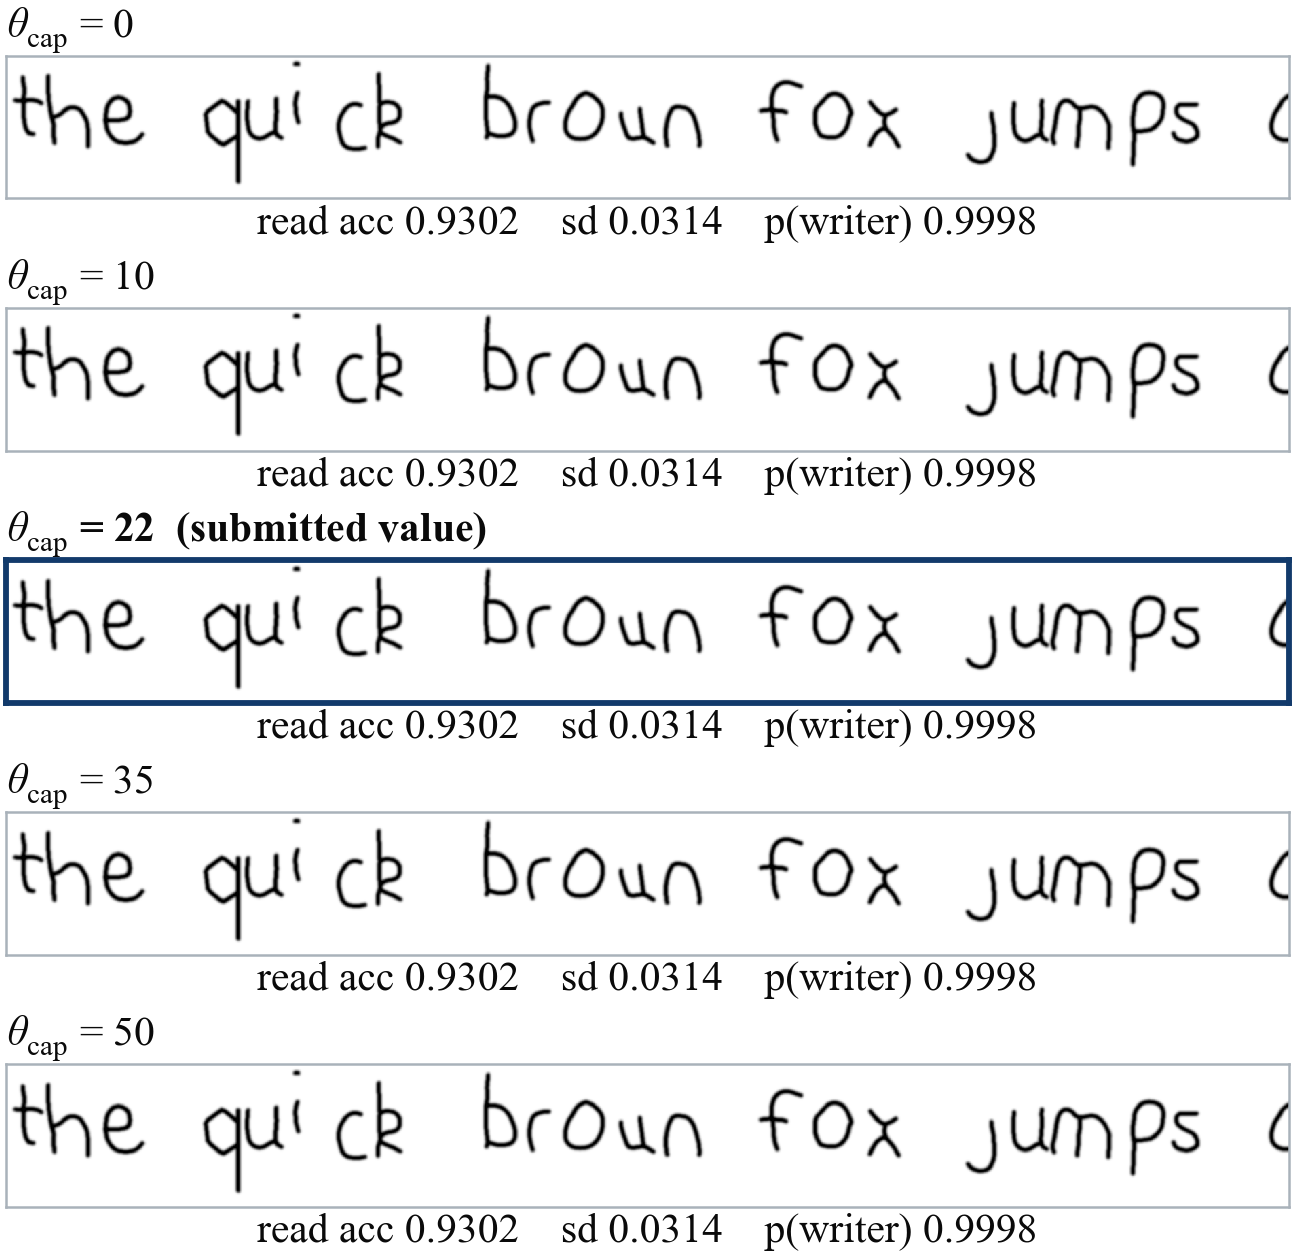
\includegraphics[width=\linewidth]{../figures/core_slant_cap.png}

\caption{Largest lean a fallback letterform is drawn at. Each panel is the same input processed by the submitted code with only $\theta_{\text{cap}}$ changed; the panel outlined in dark blue is the submitted value.}

\label{fig:core-slant-cap}

\end{figure}

\begin{figure}[htbp]

\centering

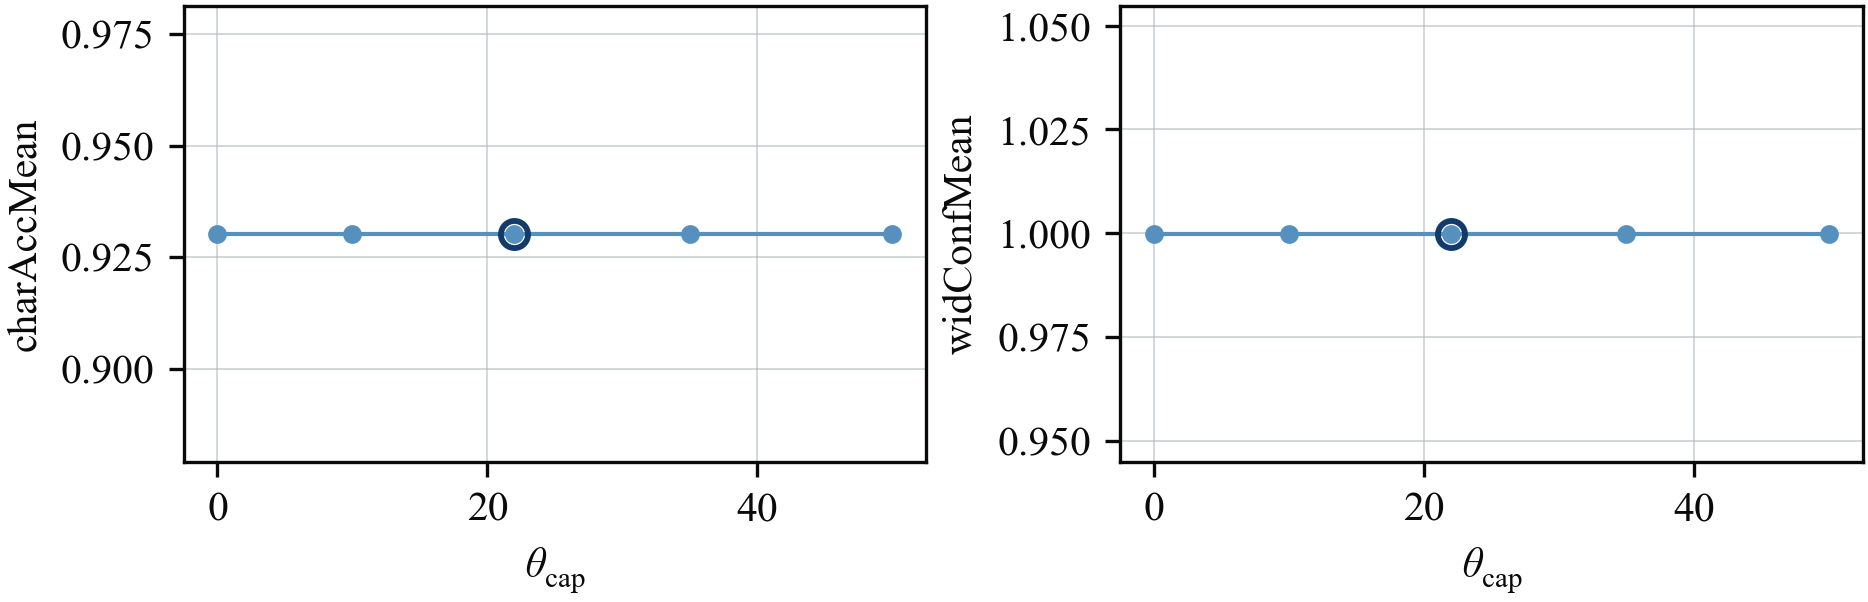
\includegraphics[width=\linewidth]{../figures/core_slant_cap_trend.png}

\caption{Largest lean a fallback letterform is drawn at: measured quantities against the swept value. The circled point is the submitted value.}

\end{figure}

\begin{table}[htbp]
\centering
\small
\caption{Largest lean a fallback letterform is drawn at: measured effect of each swept value. The submitted value is in bold.}
\begin{tabular}{lrrrr}
\toprule
\$\textbackslash\{\}theta\_\{\textbackslash\{\}text\{cap\}\}\$ & \textsf{charAccMean} & \textsf{charAccSd} & \textsf{widConfMean} & \textsf{harmonicMean} \\
\midrule
0 & 0.9302 & 0.0314 & 0.9998 & 0.9635 \\
10 & 0.9302 & 0.0314 & 0.9998 & 0.9635 \\
\bfseries 22 & \bfseries 0.9302 & \bfseries 0.0314 & \bfseries 0.9998 & \bfseries 0.9635 \\
35 & 0.9302 & 0.0314 & 0.9998 & 0.9635 \\
50 & 0.9302 & 0.0314 & 0.9998 & 0.9635 \\
\bottomrule
\end{tabular}
\end{table}

\section{Synthesis: legibility}

\subsection{Prior distance at which a writer's glyph store is still fully trusted}

\label{coef:auto-lam-good}

\begin{description}[leftmargin=5.2em,style=sameline]

\item[Symbol] $\lambda_{\text{good}}$

\item[Value] \texttt{0.24}

\item[Source] \texttt{synthesise.py}, \texttt{\_AUTO\_LAM\_GOOD}

\item[Swept] \texttt{0.1}, \texttt{0.18}, \texttt{0.24}, \texttt{0.3}, \texttt{0.45}

\end{description}

\paragraph{Basis}

Trading fidelity against legibility by interpolating towards a clean prototype is the same trade a handwriting generator makes between style and content \cite{graves2013,kang2020}.

\paragraph{Why this value}

The system must write text that is both legible and in the writer's hand, and for a rough store those two goals conflict. The legibility setting $\lambda$ is derived automatically from the median prior distance of the writer's own stored shapes, ramping linearly from $0$ at $\lambda_{\text{good}}$ to $1$ at $\lambda_{\text{bad}}$. $\lambda_{\text{good}} = 0.24$ is the distance below which the stored shapes are judged to be genuine letters that need no help, and it was set from the distribution of measured median distances across the eleven writers, not from a single page.

\paragraph{What the coefficient does}

$\lambda$ feeds \texttt{\_SwapProb}, which decides per letter whether to draw the writer's own shape or the clean fallback. Lowering $\lambda_{\text{good}}$ makes the system distrust good stores and substitute fallbacks into writing that did not need them, which raises reading accuracy and lowers writer confidence: the sweep shows that trade directly, and the \texttt{glyphSources} counts show how many letters came from the writer rather than the fallback.

\paragraph{Alternatives considered}

A fixed $\lambda$ per writer set by hand, which is what the \texttt{legibility} argument still allows; or choosing per letter from the judges, which \texttt{SynthesizeJointBestOf} does as a repair pass.

\paragraph{Worked example}

Owen's median prior distance over the stored variants is recorded in the profile; $\lambda = \mathrm{clip}((\text{med}-0.24)/(0.32-0.24), 0,1)$, so a median of $0.28$ gives $\lambda = 0.5$.

\paragraph{What the sweep actually showed}

\textbf{The largest effect found in the synthesis group, and it favours a value the project did not choose.} At $\lambda_{\text{good}} = 0.45$ the paired gain over the submitted $0.24$ is $+0.0407$ in reading accuracy ($10$ of $12$ seeds better, $t = +4.26$) and $+0.0217$ on the joint score ($11$ better, $1$ worse, $t = +4.21$). The explanation matters more than the number. The submitted $\lambda_{\text{bad}}$ is $0.32$, so setting $\lambda_{\text{good}} = 0.45$ puts the two bounds the wrong way round; the ramp $(\mathrm{med}-\lambda_{\text{good}})/(\lambda_{\text{bad}}-\lambda_{\text{good}})$ then has a negative denominator and saturates at $\lambda = 1$ for any ordinary median. $\lambda = 1$ means \emph{always substitute the clean fallback letterform}. So what this result really says is that for Owen, drawing every letter from his own most typical medoid form scores better on both judges than drawing from his stored variants --- which is a finding about the quality of the glyph store, not an argument for an inverted parameterisation. It also exposes that nothing in the code checks $\lambda_{\text{good}} < \lambda_{\text{bad}}$; at exactly $0.32$ the ramp divides by zero, which is why that point had to be moved out of this sweep. The submitted ordering is the sane one and $0.24$ is not refuted as a boundary; what is called into question is whether this writer's stored variants should be trusted at all.

\begin{figure}[htbp]

\centering

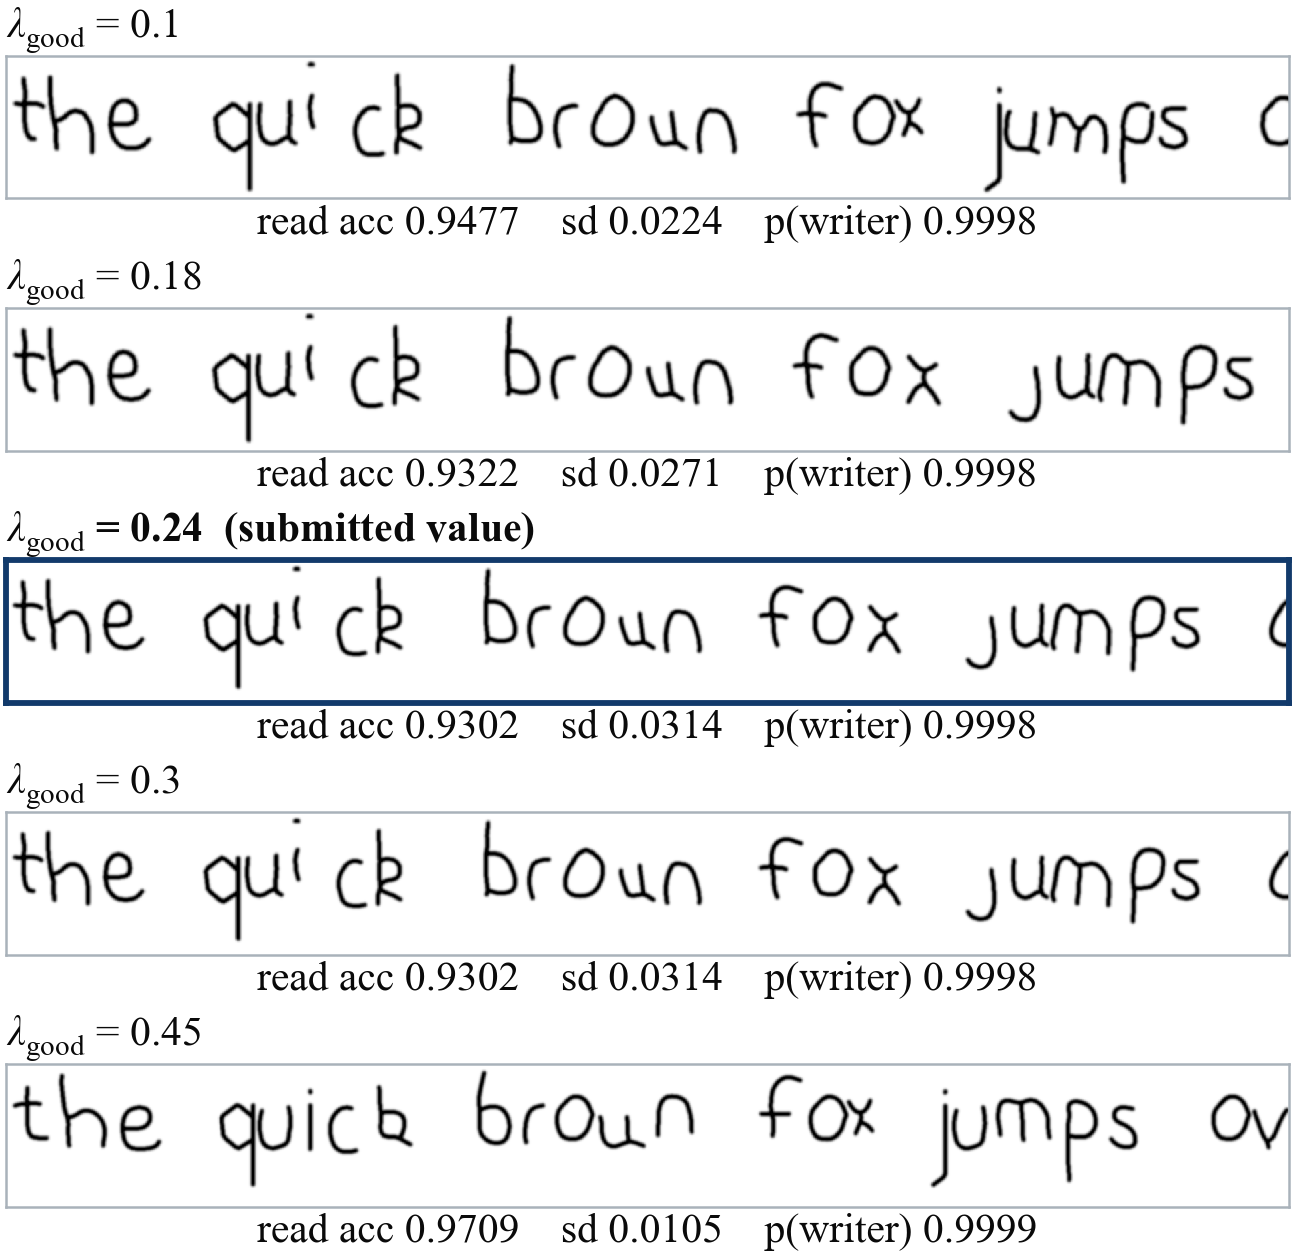
\includegraphics[width=\linewidth]{../figures/auto_lam_good.png}

\caption{Prior distance at which a writer's glyph store is still fully trusted. Each panel is the same input processed by the submitted code with only $\lambda_{\text{good}}$ changed; the panel outlined in dark blue is the submitted value.}

\label{fig:auto-lam-good}

\end{figure}

\begin{figure}[htbp]

\centering

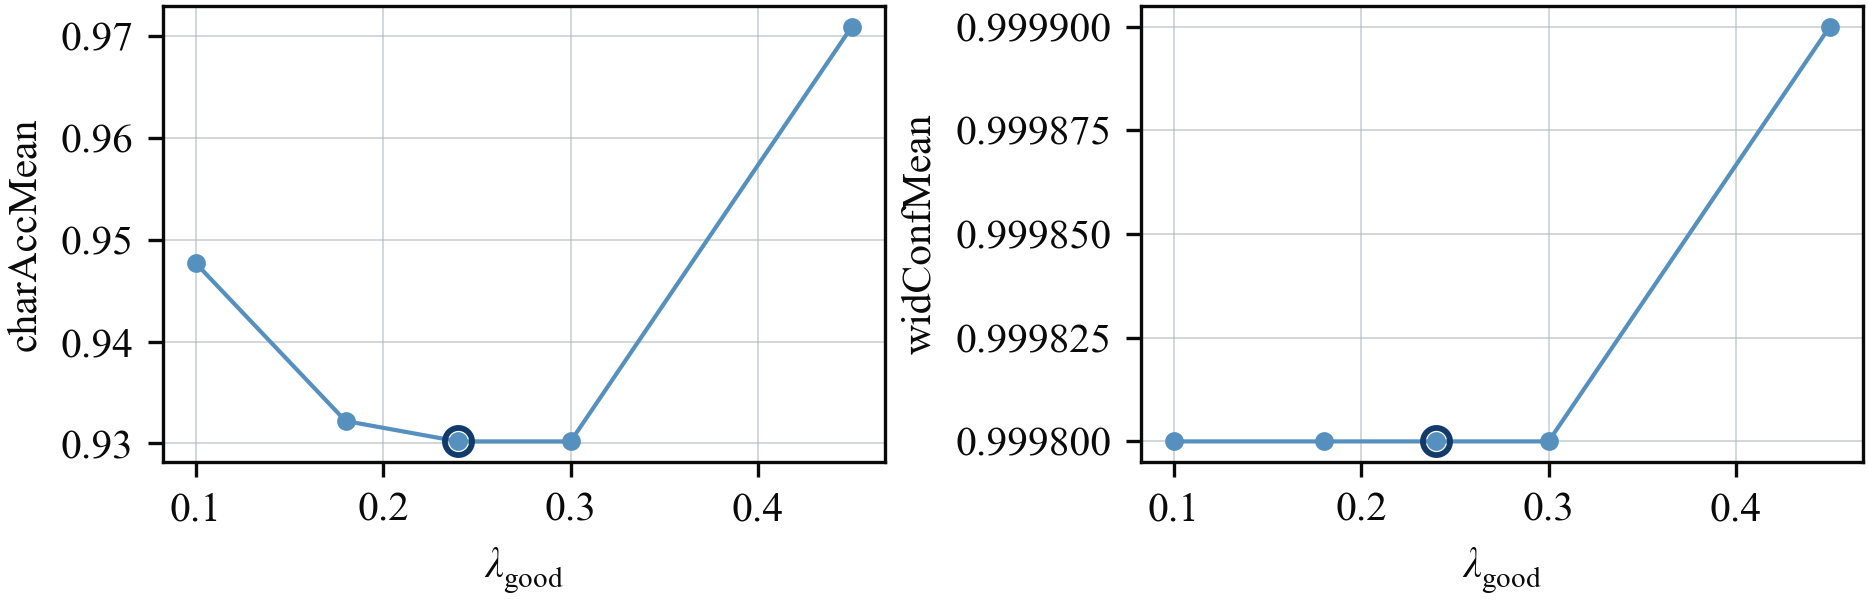
\includegraphics[width=\linewidth]{../figures/auto_lam_good_trend.png}

\caption{Prior distance at which a writer's glyph store is still fully trusted: measured quantities against the swept value. The circled point is the submitted value.}

\end{figure}

\begin{table}[htbp]
\centering
\small
\caption{Prior distance at which a writer's glyph store is still fully trusted: measured effect of each swept value. The submitted value is in bold.}
\begin{tabular}{lrrrr}
\toprule
\$\textbackslash\{\}lambda\_\{\textbackslash\{\}text\{good\}\}\$ & \textsf{charAccMean} & \textsf{charAccSd} & \textsf{widConfMean} & \textsf{harmonicMean} \\
\midrule
0.1 & 0.9477 & 0.0224 & 0.9998 & 0.9729 \\
0.18 & 0.9322 & 0.0271 & 0.9998 & 0.9646 \\
\bfseries 0.24 & \bfseries 0.9302 & \bfseries 0.0314 & \bfseries 0.9998 & \bfseries 0.9635 \\
0.3 & 0.9302 & 0.0314 & 0.9998 & 0.9635 \\
0.45 & 0.9709 & 0.0105 & 0.9999 & 0.9852 \\
\bottomrule
\end{tabular}
\end{table}

\section{G-code generation}

\subsection{Gap the pen draws through instead of lifting}

\label{coef:join-strokes-mm}

\begin{description}[leftmargin=5.2em,style=sameline]

\item[Symbol] $d_{\text{join}}$

\item[Value] \texttt{0.6}

\item[Source] \texttt{reproduce.py}, \texttt{GantryConfig.joinStrokesMm}

\item[Swept] \texttt{0.0}, \texttt{0.25}, \texttt{0.6}, \texttt{1.5}, \texttt{4.0}

\end{description}

\paragraph{Basis}

Minimising non-productive moves and tool changes is the standard objective of toolpath generation; the pen-up and pen-down commands themselves are the \texttt{M3}/\texttt{M5} spindle words of \cite{iso6983}.

\paragraph{Why this value}

Lifting the pen costs far more than drawing a short line: each lift is two pen pulses, each with a $350$ ms dwell, so $0.7$ s, while drawing $0.6$ mm at the $900$ mm/min drawing feed costs $0.04$ s. Where the next stroke begins very close to where the last one ended, drawing straight into it is therefore about twenty times faster, and it also removes the risk that the pen fails to re-seat. The cost is a visible mark: the gap is drawn as ink, so $d_{\text{join}}$ must stay below the width at which that mark is noticeable. At $0.6$ mm the added line is comparable with the pen's own $0.7$ mm trace and reads as part of the stroke.

\paragraph{What the coefficient does}

The statistics make the trade explicit: \texttt{joinedStrokes} counts how many lifts were avoided and \texttt{joinedInkMm} how much ink was added to avoid them. Raising $d_{\text{join}}$ draws ever longer false connections across the writing; at $0$ every stroke gets its own lift.

\paragraph{Alternatives considered}

Reordering strokes so that consecutive ones start near each other, which \texttt{OptimizeStrokeOrder} already does, or a faster pen actuator, which is a hardware change.

\paragraph{Worked example}

One avoided lift saves $2 \times 350 = 700$ ms of dwell plus the travel move, and costs at most $0.6$ mm of ink drawn at $900$ mm/min, which is $0.04$ s.

\paragraph{What the sweep actually showed}

This sweep quantifies the trade exactly, and it is the clearest cost--benefit result in the study. On the probe job:\begin{center}\small\begin{tabular}{rrrrr}\toprule$d_{\text{join}}$ & pen pulses & joins & ink added & estimated time \\\midrule$0.0$ & $52$ & $0$ & $0.0$ mm & $30.9$ s \\$0.25$ & $52$ & $0$ & $0.0$ mm & $30.9$ s \\$\mathbf{0.6}$ & $\mathbf{48}$ & $\mathbf{2}$ & $\mathbf{0.8}$ mm & $\mathbf{29.5}$ s \\$1.5$ & $40$ & $6$ & $5.6$ mm & $26.9$ s \\$4.0$ & $14$ & $19$ & $37.5$ mm & $19.1$ s \\\bottomrule\end{tabular}\end{center}The submitted value buys back $1.4$ s for $0.8$ mm of added ink across the whole job, which is about one pen width and is not visible. At $4.0$ mm the saving is far larger --- $11.8$ s, $38\,\%$ of the job --- but it costs $37.5$ mm of ink drawn across the writing in lines up to $4$ mm long, which is a whole letter width and would be obvious. So the coefficient is not set where the time saving is greatest; it is set at the largest gap that still hides inside the stroke. That is the right criterion, and the table is the evidence for it.

\begin{figure}[htbp]

\centering

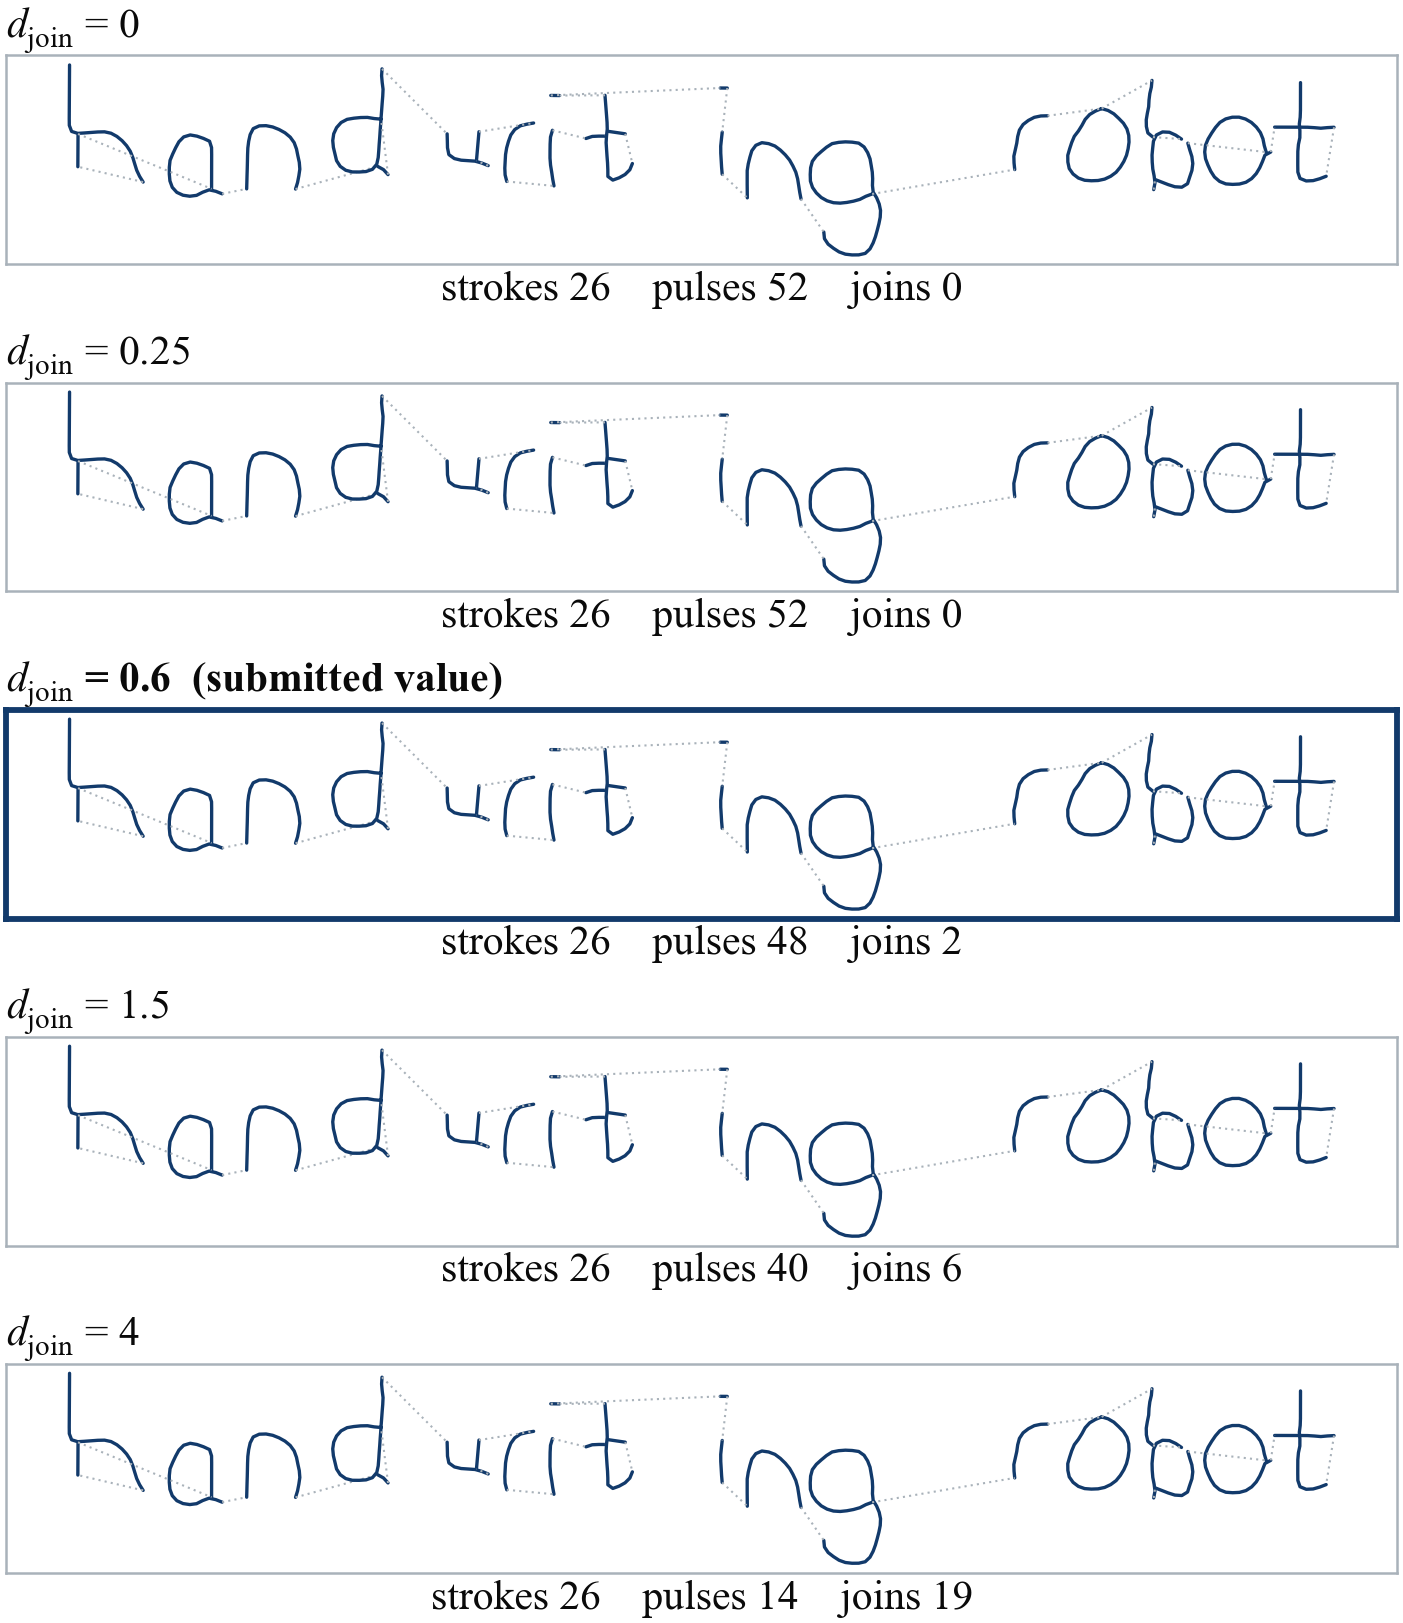
\includegraphics[width=\linewidth]{../figures/join_strokes_mm.png}

\caption{Gap the pen draws through instead of lifting. Each panel is the same input processed by the submitted code with only $d_{\text{join}}$ changed; the panel outlined in dark blue is the submitted value.}

\label{fig:join-strokes-mm}

\end{figure}

\begin{figure}[htbp]

\centering

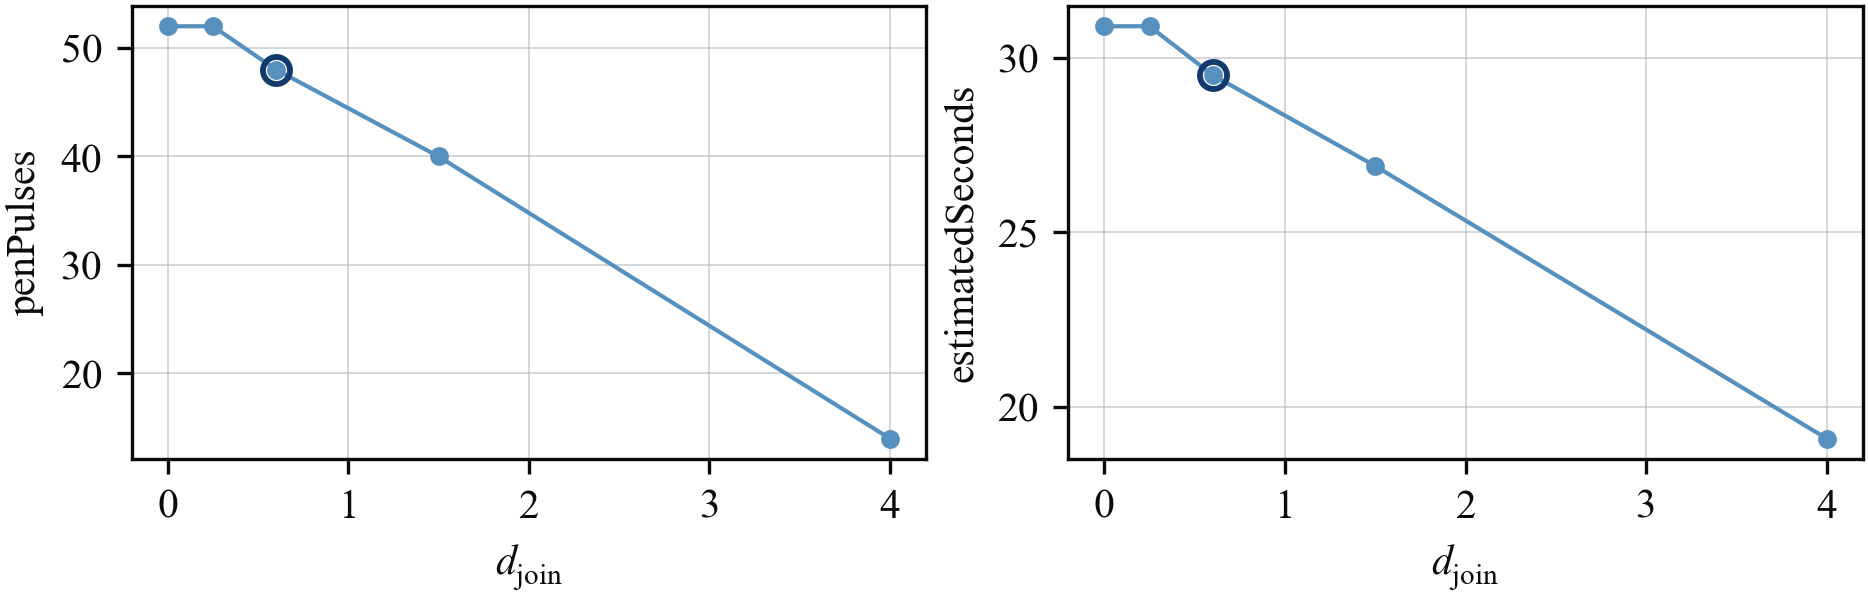
\includegraphics[width=\linewidth]{../figures/join_strokes_mm_trend.png}

\caption{Gap the pen draws through instead of lifting: measured quantities against the swept value. The circled point is the submitted value.}

\end{figure}

\begin{table}[htbp]
\centering
\small
\caption{Gap the pen draws through instead of lifting: measured effect of each swept value. The submitted value is in bold.}
\begin{tabular}{lrrrrrr}
\toprule
\$d\_\{\textbackslash\{\}text\{join\}\}\$ & \textsf{strokes} & \textsf{penPulses} & \textsf{joinedStrokes} & \textsf{joinedInkMm} & \textsf{travelMm} & \textsf{estimatedSeconds} \\
\midrule
0 & 26 & 52 & 0 & 0 & 153.9 & 30.9 \\
0.25 & 26 & 52 & 0 & 0 & 153.9 & 30.9 \\
\bfseries 0.6 & \bfseries 26 & \bfseries 48 & \bfseries 2 & \bfseries 0.8 & \bfseries 153.1 & \bfseries 29.5 \\
1.5 & 26 & 40 & 6 & 5.6 & 148.3 & 26.9 \\
4 & 26 & 14 & 19 & 37.52 & 116.4 & 19.1 \\
\bottomrule
\end{tabular}
\end{table}

\subsection{Gap at which a stroke is closed into a ring}

\label{coef:close-ring-mm}

\begin{description}[leftmargin=5.2em,style=sameline]

\item[Symbol] $d_{\text{ring}}$

\item[Value] \texttt{0.6}

\item[Source] \texttt{reproduce.py}, \texttt{GantryConfig.closeRingMm}

\item[Swept] \texttt{0.0}, \texttt{0.25}, \texttt{0.6}, \texttt{1.5}, \texttt{4.0}

\end{description}

\paragraph{Basis}

Closing a nearly closed contour is the standard repair for a traced loop whose ends do not meet after thinning \cite{lam1992}.

\paragraph{Why this value}

A letter with a loop, such as \texttt{o}, \texttt{a} or \texttt{e}, is traced from a skeleton whose ends rarely meet exactly: thinning and simplification leave a gap of a fraction of a millimetre. Drawn as-is the loop has a visible notch. If a stroke's own two ends are within $d_{\text{ring}}$, the first point is appended so the ring closes. The limit is the same $0.6$ mm as the join limit for the same reason: it is about one pen width, so closing is invisible.

\paragraph{What the coefficient does}

The test applies only to a stroke's own ends and only when it has more than three points, so it cannot close a short two-point dash into a degenerate ring. Too large and a genuine \texttt{c}, whose ends are meant to be apart, is closed into an \texttt{o}, which is a legibility error, not just a cosmetic one.

\paragraph{Alternatives considered}

Closing in the glyph store rather than at G-code time, which would record the closure in the profile and make it visible to the shape descriptor; or never closing and accepting the notch.

\paragraph{Worked example}

At $4$ mm per x-height an \texttt{o} is about $3$ mm across, so $0.6$ mm is a fifth of the letter: a \texttt{c} with a normal opening is well outside the limit.

\paragraph{What the sweep actually showed}

The ring count rises $0$, $1$, $1$, $4$, $20$ across the sweep and the drawn length rises with it, $133.0$, $133.3$, $133.3$, $135.5$, $179.0$ mm. The last value is the warning: at $4.0$ mm every one of the job's $20$ remaining strokes is closed into a ring, the drawn length grows by $34\,\%$ over the submitted setting, and the job gets \emph{slower} ($34.6$ s against $29.5$ s) as well as wrong, because letters such as \texttt{c} that are meant to be open are sealed shut. The submitted $0.6$ closes exactly one genuine loop and adds $0.3$ mm.

\begin{figure}[htbp]

\centering

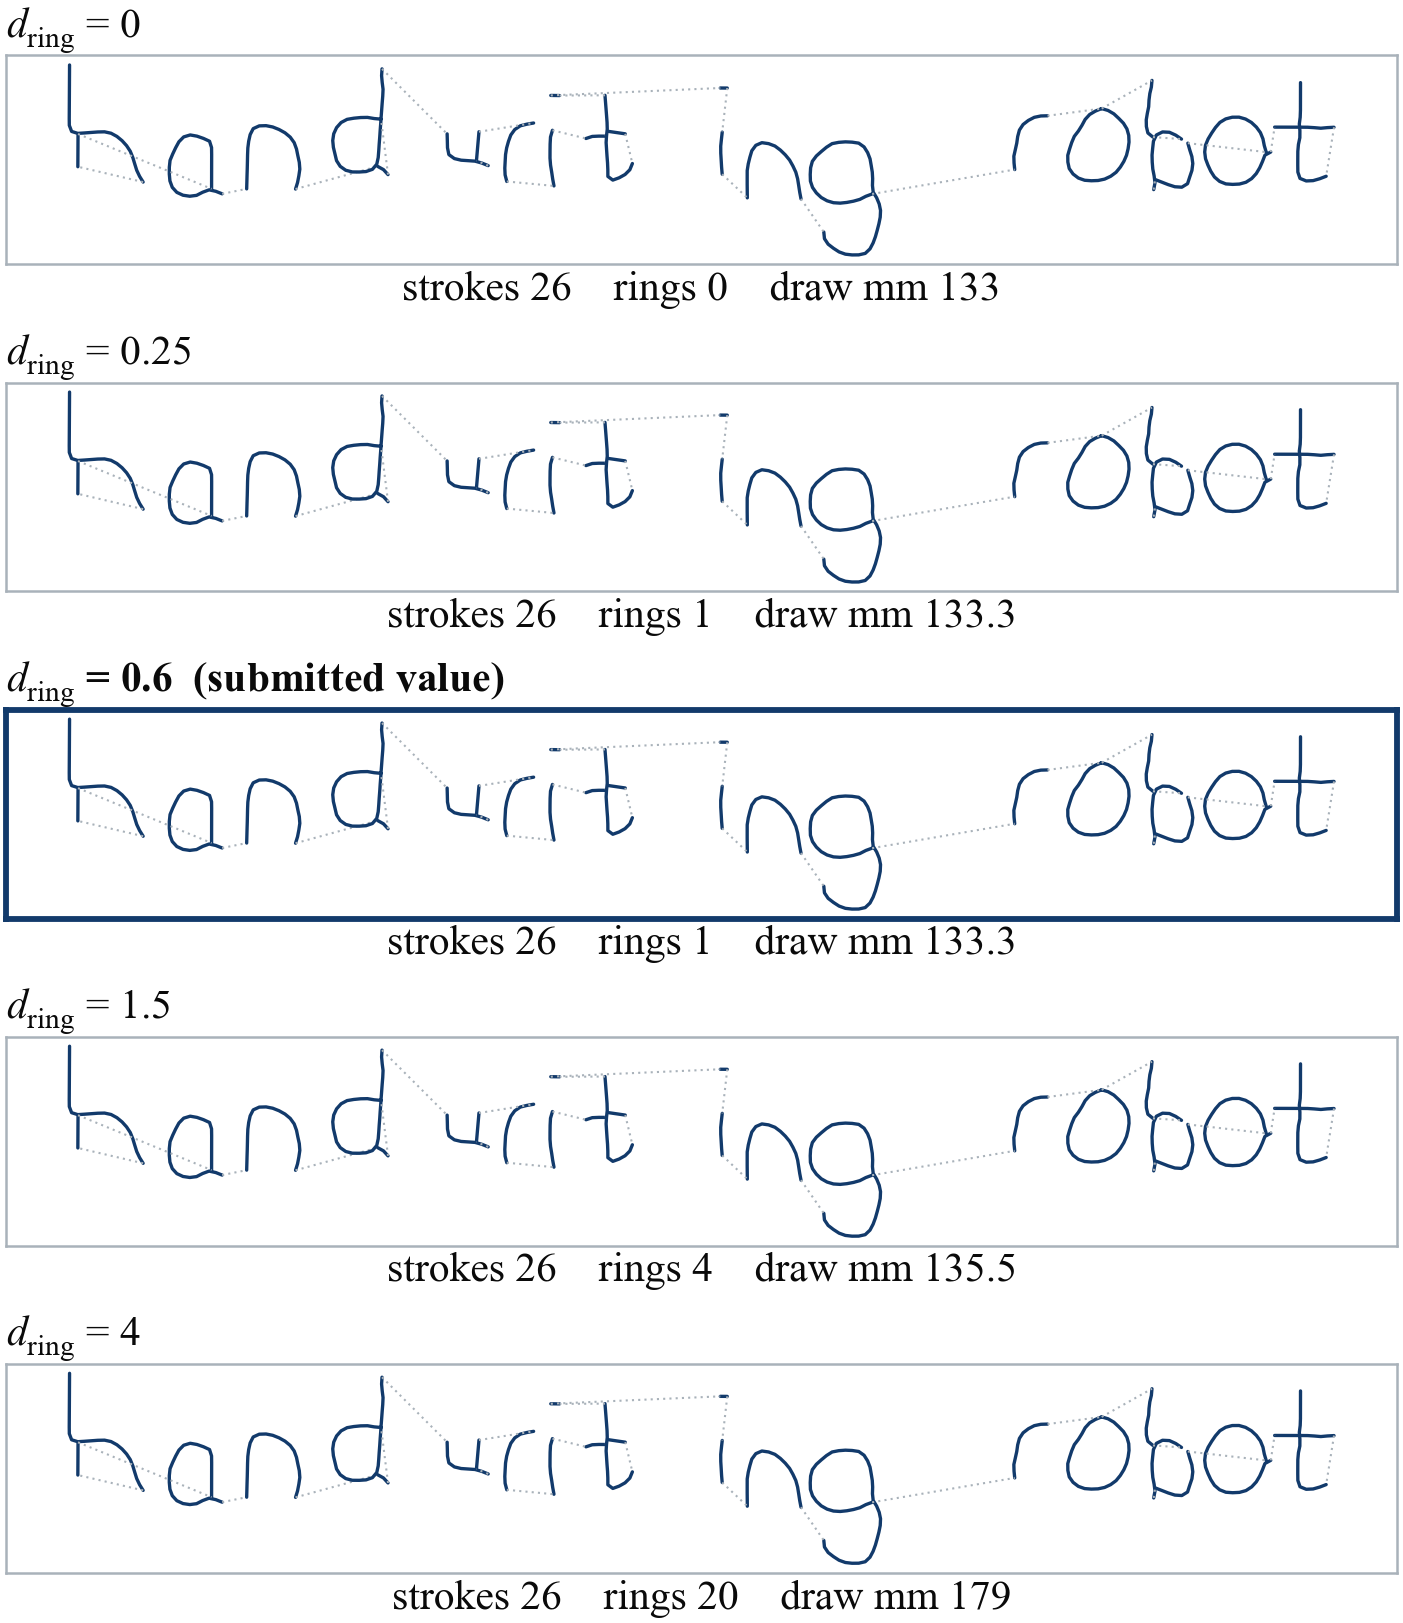
\includegraphics[width=\linewidth]{../figures/close_ring_mm.png}

\caption{Gap at which a stroke is closed into a ring. Each panel is the same input processed by the submitted code with only $d_{\text{ring}}$ changed; the panel outlined in dark blue is the submitted value.}

\label{fig:close-ring-mm}

\end{figure}

\begin{figure}[htbp]

\centering

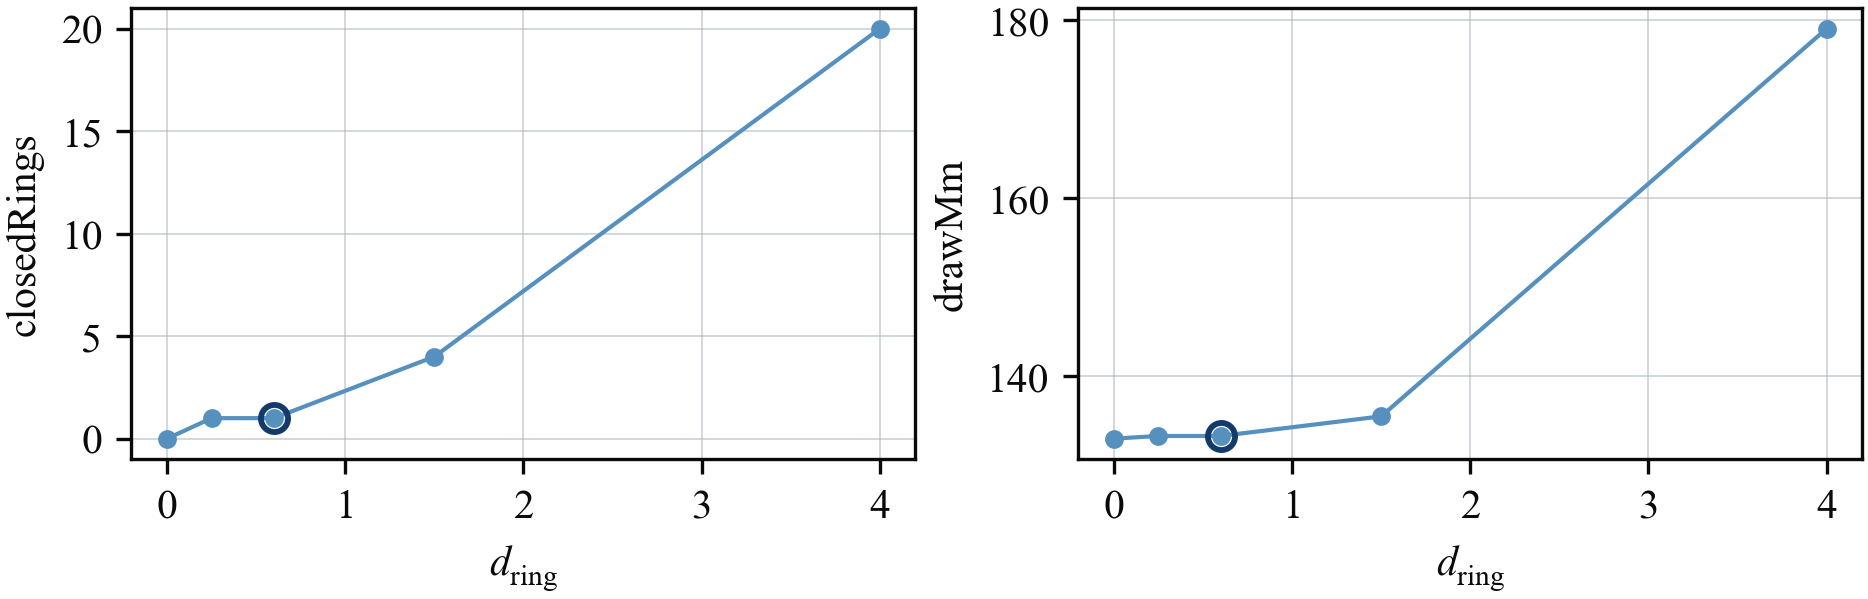
\includegraphics[width=\linewidth]{../figures/close_ring_mm_trend.png}

\caption{Gap at which a stroke is closed into a ring: measured quantities against the swept value. The circled point is the submitted value.}

\end{figure}

\begin{table}[htbp]
\centering
\small
\caption{Gap at which a stroke is closed into a ring: measured effect of each swept value. The submitted value is in bold.}
\begin{tabular}{lrrrr}
\toprule
\$d\_\{\textbackslash\{\}text\{ring\}\}\$ & \textsf{strokes} & \textsf{closedRings} & \textsf{drawMm} & \textsf{estimatedSeconds} \\
\midrule
0 & 26 & 0 & 133 & 29.5 \\
0.25 & 26 & 1 & 133.3 & 29.5 \\
\bfseries 0.6 & \bfseries 26 & \bfseries 1 & \bfseries 133.3 & \bfseries 29.5 \\
1.5 & 26 & 4 & 135.5 & 30.4 \\
4 & 26 & 20 & 179 & 34.6 \\
\bottomrule
\end{tabular}
\end{table}

\subsection{Shortest move kept in the G-code}

\label{coef:min-segment-mm}

\begin{description}[leftmargin=5.2em,style=sameline]

\item[Symbol] $\ell_{\min}$

\item[Value] \texttt{0.12}

\item[Source] \texttt{reproduce.py}, \texttt{GantryConfig.minSegmentMm}

\item[Swept] \texttt{0.0}, \texttt{0.05}, \texttt{0.12}, \texttt{0.3}, \texttt{1.0}

\end{description}

\paragraph{Basis}

Chord tolerance and minimum segment length are standard parameters of toolpath post-processing; the machine resolution they are set against follows from the microstepping of the driver \cite{a4988ds} and the motor step angle \cite{stepperds}.

\paragraph{Why this value}

There is no point emitting a move the machine cannot resolve. One microstep is $40/(200 \times 16) = 0.0125$ mm, so moves below about that are rounded to nothing by \texttt{\_GcodeLinearMove}, which rounds target positions to whole steps. $\ell_{\min} = 0.12$ mm is about ten microsteps: comfortably resolvable, but small against a $4$ mm x-height, so discarding shorter moves does not visibly change a letter. The benefit is file size and interpreter time, which matter because the G-code is parsed line by line in Python on the ODROID.

\paragraph{What the coefficient does}

\texttt{\_Decimate} always keeps the first and last point of a stroke, so decimation cannot shorten a stroke or move its endpoints; it only drops intermediate points. Raising $\ell_{\min}$ progressively straightens curves, which is visible on a letter before it is visible in the statistics.

\paragraph{Alternatives considered}

A chord-deviation tolerance, as Douglas--Peucker \cite{douglas1973} applies in the glyph store, which is shape-aware rather than length-based and would be the better criterion here too; or no decimation.

\paragraph{Worked example}

At $0.12$ mm and a drawing feed of $900$ mm/min, one retained segment takes $8$ ms. The probe job emits the recorded number of G-code lines at each setting.

\paragraph{What the sweep actually showed}

\textbf{The submitted value does nothing on this job.} The generated file is $533$ lines at $\ell_{\min} = 0$, $0.05$, $0.12$ and $0.3$ alike, and only at $1.0$ mm does decimation bite, cutting the file to $286$ lines, a $46\,\%$ reduction, while shortening the drawn path from $133.3$ to $130.4$ mm. The reason is that the points reaching the G-code writer are already further apart than $0.12$ mm, because \texttt{SmoothStroke} resamples at $0.055$ x-heights, which at this size is $0.22$ mm. So the decimation is a guard that is never reached rather than an active size reduction, and the file-size argument given for it above is not supported on this job. Setting it near $1.0$ mm would halve the file, at a visible cost in curve fidelity.

\begin{figure}[htbp]

\centering

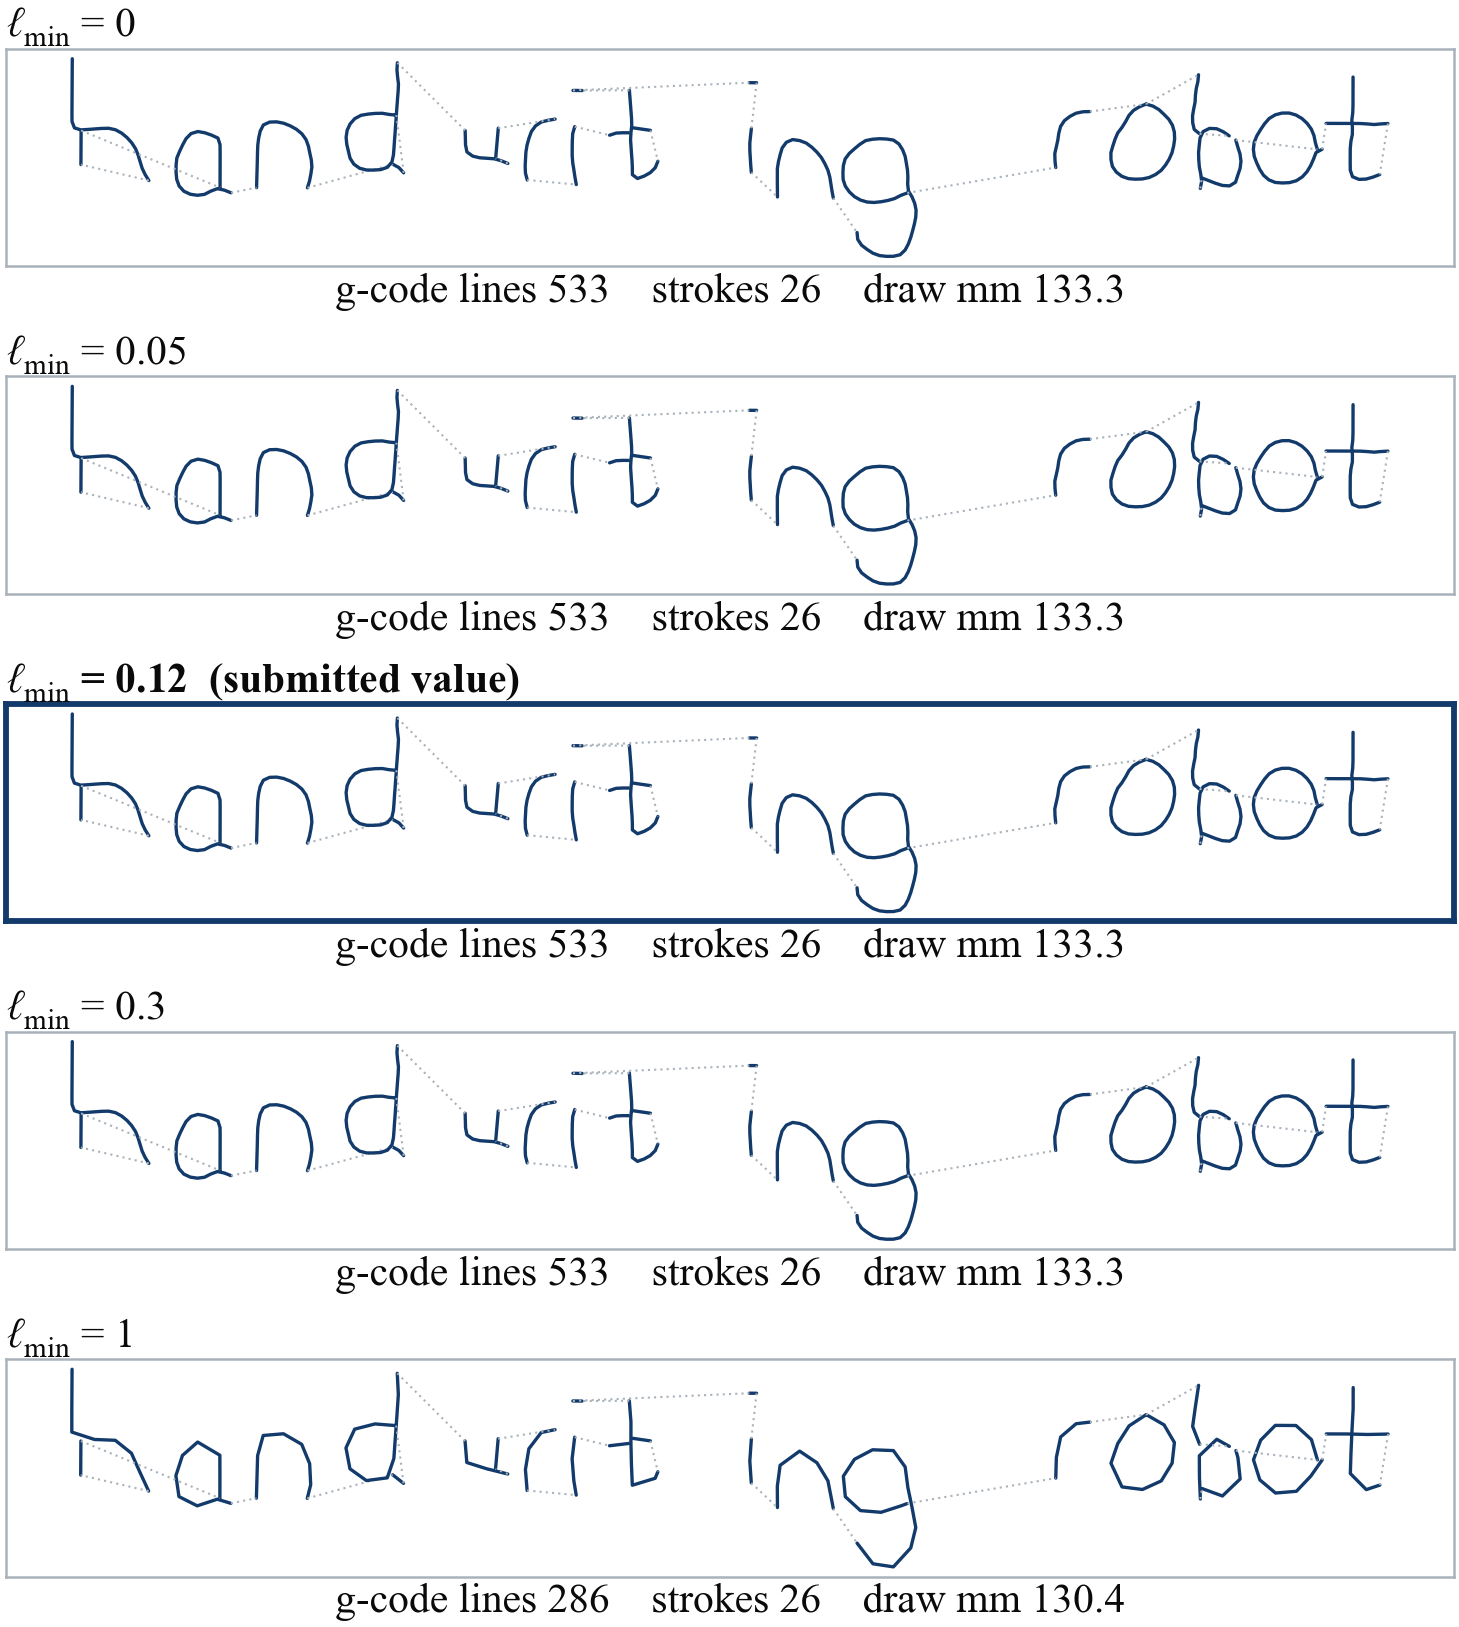
\includegraphics[width=\linewidth]{../figures/min_segment_mm.png}

\caption{Shortest move kept in the G-code. Each panel is the same input processed by the submitted code with only $\ell_{\min}$ changed; the panel outlined in dark blue is the submitted value.}

\label{fig:min-segment-mm}

\end{figure}

\begin{figure}[htbp]

\centering

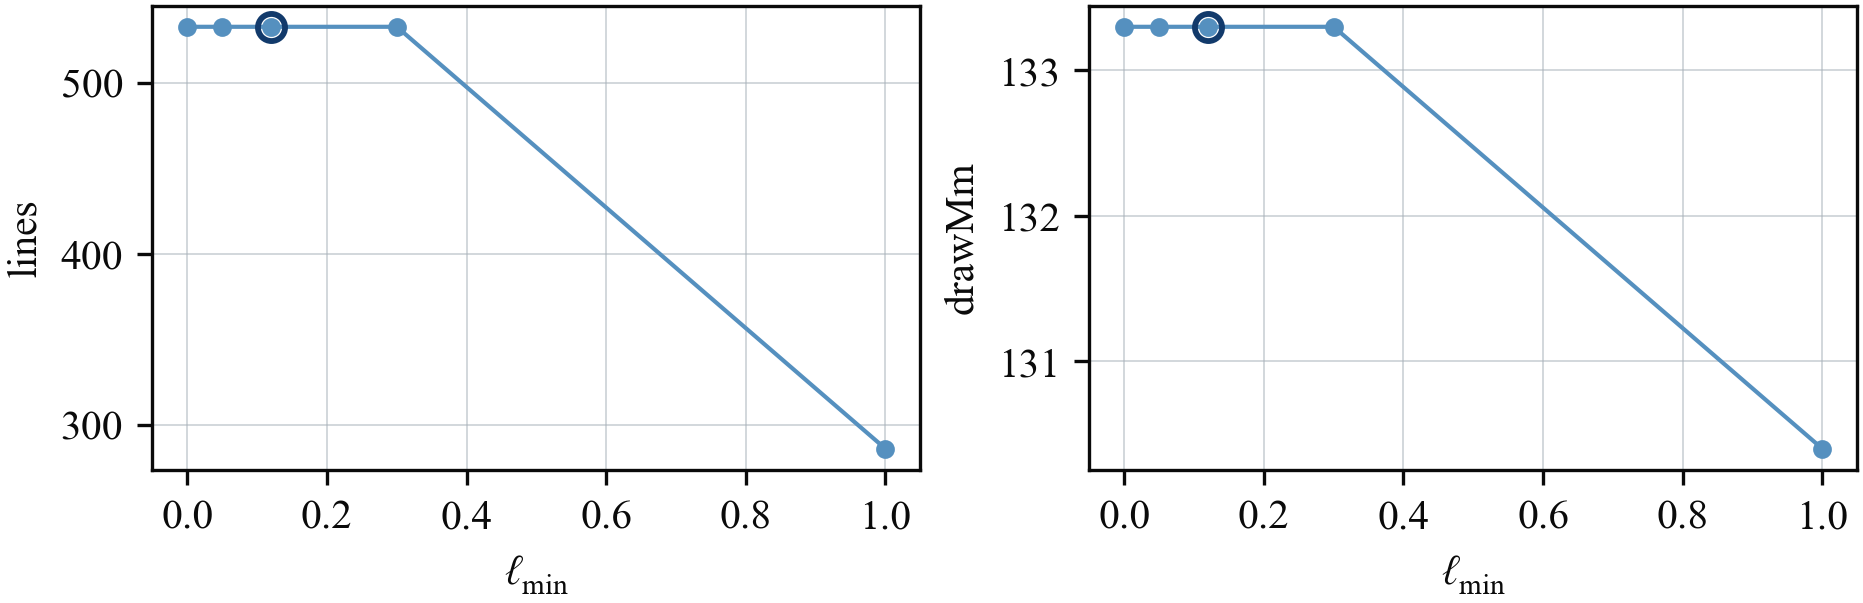
\includegraphics[width=\linewidth]{../figures/min_segment_mm_trend.png}

\caption{Shortest move kept in the G-code: measured quantities against the swept value. The circled point is the submitted value.}

\end{figure}

\begin{table}[htbp]
\centering
\small
\caption{Shortest move kept in the G-code: measured effect of each swept value. The submitted value is in bold.}
\begin{tabular}{lrrrr}
\toprule
\$\textbackslash\{\}ell\_\{\textbackslash\{\}min\}\$ & \textsf{lines} & \textsf{strokes} & \textsf{drawMm} & \textsf{estimatedSeconds} \\
\midrule
0 & 533 & 26 & 133.3 & 29.5 \\
0.05 & 533 & 26 & 133.3 & 29.5 \\
\bfseries 0.12 & \bfseries 533 & \bfseries 26 & \bfseries 133.3 & \bfseries 29.5 \\
0.3 & 533 & 26 & 133.3 & 29.5 \\
1 & 286 & 26 & 130.4 & 29.3 \\
\bottomrule
\end{tabular}
\end{table}

\section{Pen actuator}

\subsection{Dwell after a pen-down pulse}

\label{coef:pen-dwell-ms}

\begin{description}[leftmargin=5.2em,style=sameline]

\item[Symbol] $t_{\text{down}}$

\item[Value] \texttt{350.0}

\item[Source] \texttt{reproduce.py}, \texttt{GantryConfig.penDownDwellMs}

\item[Swept] \texttt{100.0}, \texttt{200.0}, \texttt{350.0}, \texttt{500.0}, \texttt{800.0}

\end{description}

\paragraph{Basis}

A dwell is the \texttt{G4} word of \cite{iso6983}. The need for one follows from the actuator being an uncontrolled one-way gear motor rather than a servo: there is no position feedback to wait on, so the wait must be open-loop.

\paragraph{Why this value}

The pen is raised and lowered by a gear motor that turns $90^\circ$ per pulse and cannot be commanded to a position. The controller therefore issues the pulse and waits long enough for the rotation to finish and the nib to settle before any motion command follows. If the wait is too short the carriage starts moving while the pen is still descending and the first few millimetres of the stroke are drawn faint or not at all, which is the pen-pressure fault this project has recorded. The down dwell is held equal to the up dwell at $350$ ms, with the comment in the source noting it is the longer case because the nib must seat.

\paragraph{What the coefficient does}

The dwell is pure cost: it is paid twice per pen cycle and the estimate counts $\text{pulses} \times (t_{\text{up}}+t_{\text{down}})/2$. On a job with $58$ pulses it accounts for $58 \times 0.35 = 20.3$ s of a $34.1$ s estimate, that is $60\%$ of the predicted job time. That makes it the single largest term in the time budget and the first thing to attack for speed.

\paragraph{Alternatives considered}

Reading the pen switch and continuing as soon as it confirms, which the code already does inside \texttt{SetPen} with a $3$ s timeout and a $40$ ms overrun, so the dwell is a second, open-loop guard on top of a closed-loop wait; a sprung pen holder, which removes the need to wait at all; or a servo with position feedback.

\paragraph{Worked example}

On the probe job the submitted setting gives $48 \times (350+350)/2000 = 16.8$ s of dwell against $8.9$ s of drawing and $3.8$ s of travel, that is $57\%$ of a $29.5$ s estimate.

\paragraph{What the sweep actually showed}

The dwell dominates the predicted job time, as claimed. Dwell seconds run $10.8$, $13.2$, $16.8$, $20.4$, $27.6$ against a drawing time fixed at $8.9$ s and a travel time of $3.8$ s, so the estimate runs $23.5$, $25.9$, $29.5$, $33.1$, $40.3$ s. At the submitted $350$ ms the dwell is $16.8$ s of a $29.5$ s job, which is \textbf{$57\,\%$ of the predicted time spent waiting for the pen}. Halving it to $175$ ms would take about $4$ s off this job. That makes the pen actuator, not the motion, the thing to attack for speed --- but nothing here says $350$ ms is longer than the nib needs, because no gantry was run. The sweep bounds the prize; a timed test on the machine would say whether it can be claimed.

\paragraph{Limits of this test}

This sweep is arithmetic on the generated job, not a measurement of the machine: no gantry was run. Whether $350$ ms is actually long enough for the nib to seat is a hardware question that needs a timed test on the gantry, and that test has not been done.

\begin{figure}[htbp]

\centering

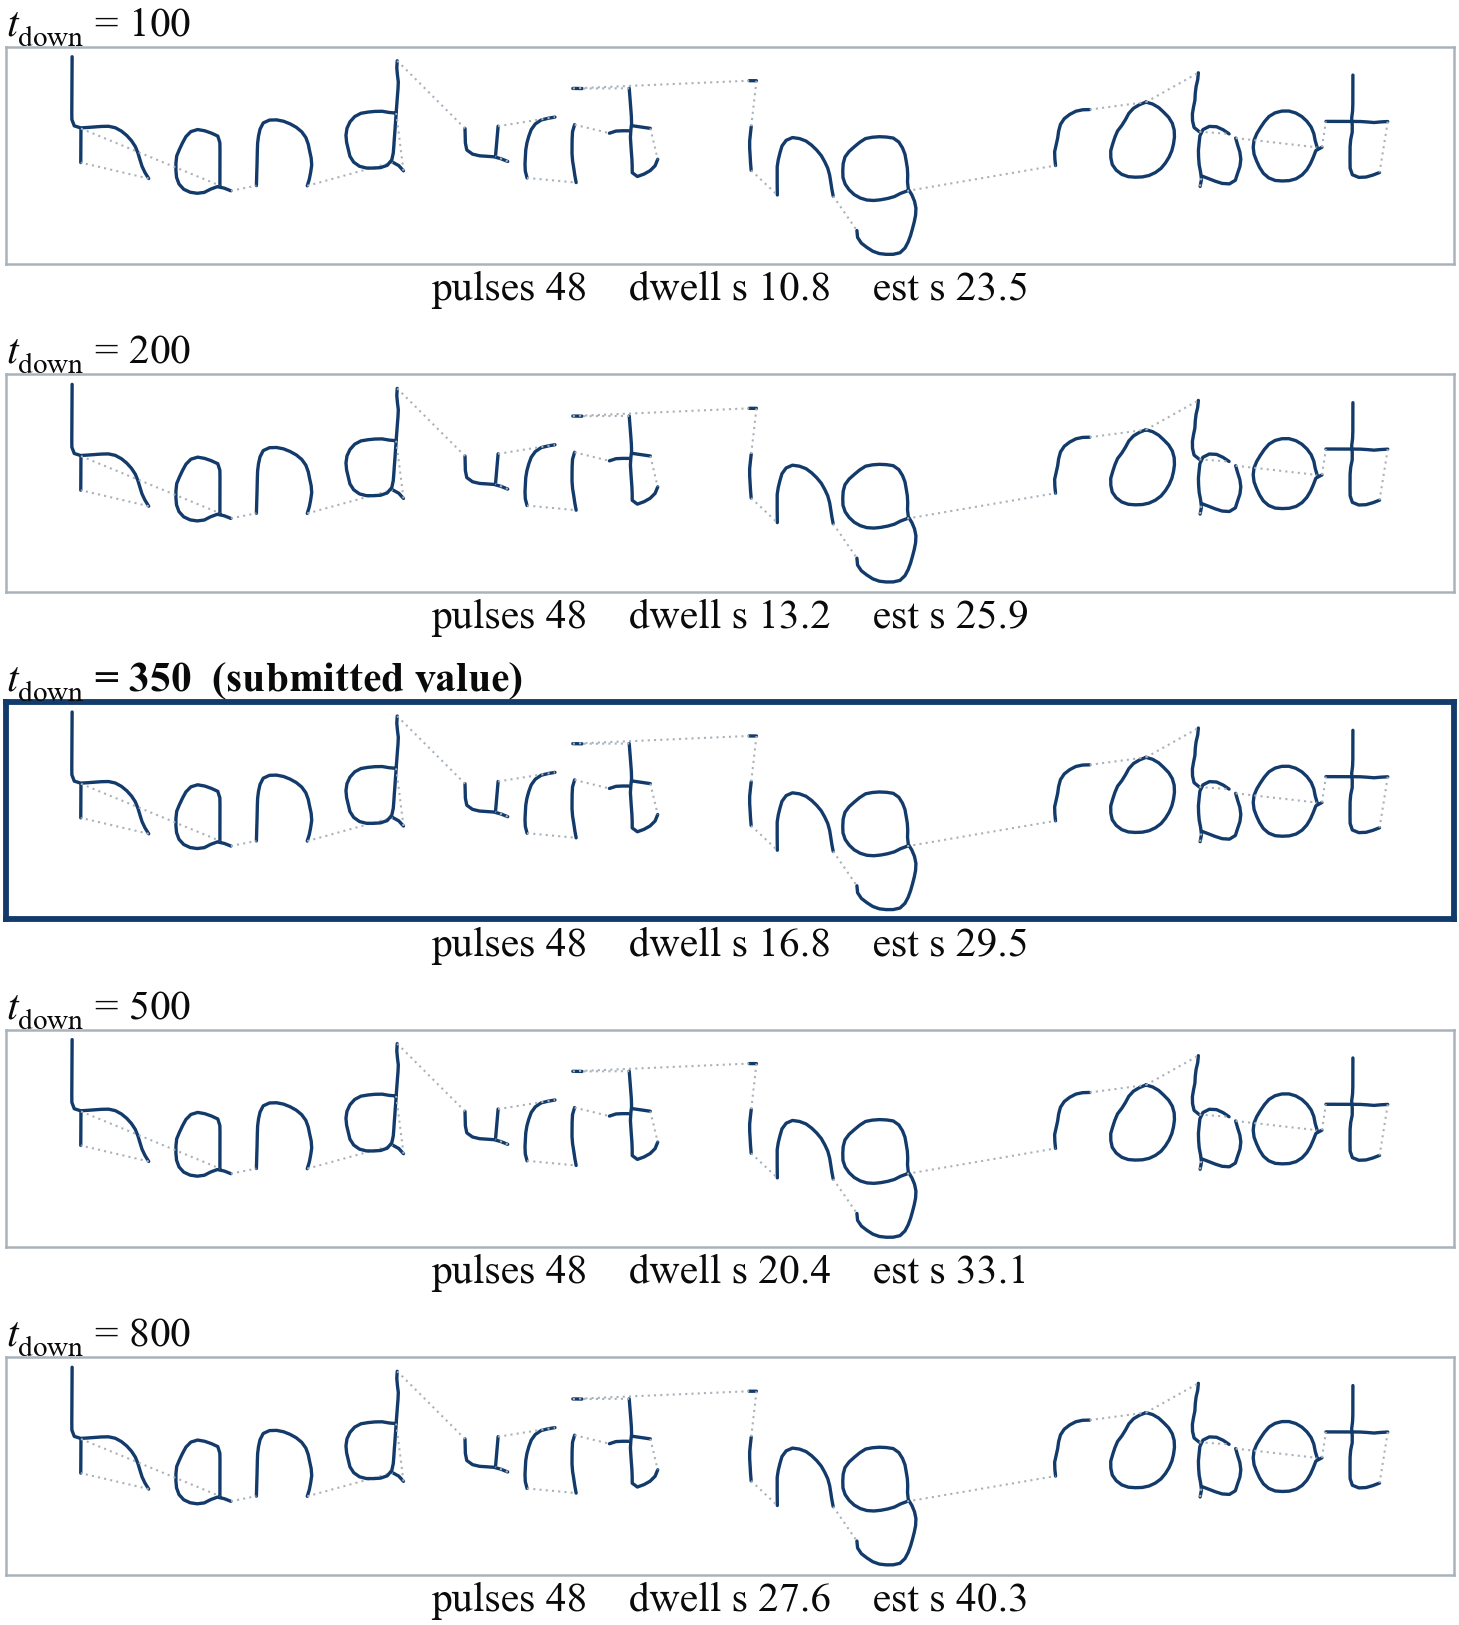
\includegraphics[width=\linewidth]{../figures/pen_dwell_ms.png}

\caption{Dwell after a pen-down pulse. Each panel is the same input processed by the submitted code with only $t_{\text{down}}$ changed; the panel outlined in dark blue is the submitted value.}

\label{fig:pen-dwell-ms}

\end{figure}

\begin{figure}[htbp]

\centering

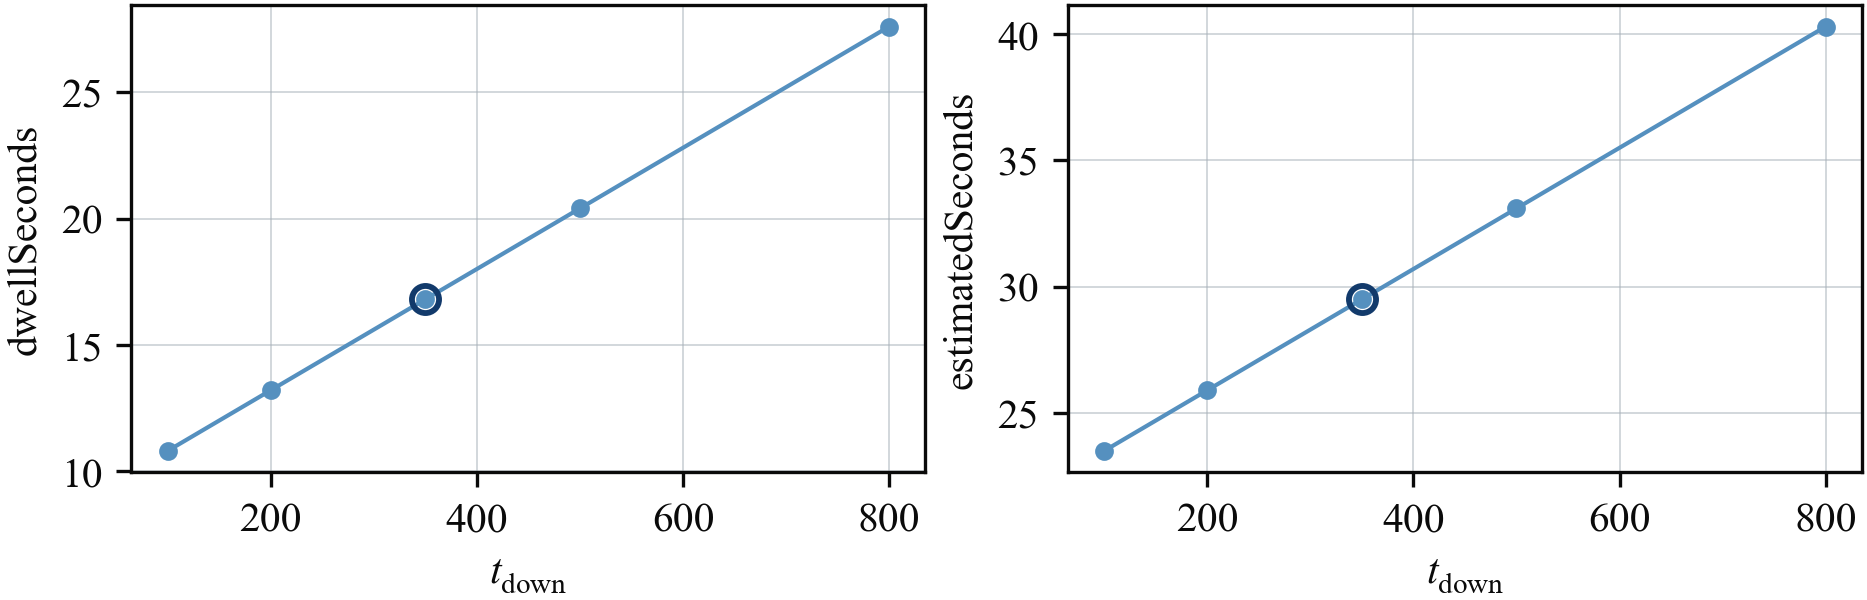
\includegraphics[width=\linewidth]{../figures/pen_dwell_ms_trend.png}

\caption{Dwell after a pen-down pulse: measured quantities against the swept value. The circled point is the submitted value.}

\end{figure}

\begin{table}[htbp]
\centering
\small
\caption{Dwell after a pen-down pulse: measured effect of each swept value. The submitted value is in bold.}
\begin{tabular}{lrrrr}
\toprule
\$t\_\{\textbackslash\{\}text\{down\}\}\$ & \textsf{penPulses} & \textsf{dwellSeconds} & \textsf{estimatedSeconds} & \textsf{drawSeconds} \\
\midrule
100 & 48 & 10.8 & 23.5 & 8.9 \\
200 & 48 & 13.2 & 25.9 & 8.9 \\
\bfseries 350 & \bfseries 48 & \bfseries 16.8 & \bfseries 29.5 & \bfseries 8.9 \\
500 & 48 & 20.4 & 33.1 & 8.9 \\
800 & 48 & 27.6 & 40.3 & 8.9 \\
\bottomrule
\end{tabular}
\end{table}

\section{Motion}

\subsection{Feed rate while drawing}

\label{coef:draw-feed}

\begin{description}[leftmargin=5.2em,style=sameline]

\item[Symbol] $F_{\text{draw}}$

\item[Value] \texttt{900.0}

\item[Source] \texttt{reproduce.py}, \texttt{GantryConfig.drawFeedMmMin}

\item[Swept] \texttt{300.0}, \texttt{600.0}, \texttt{900.0}, \texttt{1500.0}, \texttt{2400.0}

\end{description}

\paragraph{Basis}

Feed rate is the \texttt{F} word of \cite{iso6983}. The upper bound is set by the step rate the driver and motor can follow \cite{a4988ds,stepperds}; the trapezoidal profiling that would normally bound acceleration is described by Biagiotti and Melchiorri \cite{biagiotti2008} and is \emph{not} implemented here.

\paragraph{Why this value}

$900$ mm/min is $15$ mm/s, which at $80$ steps/mm is a step rate of $1200$ Hz, well inside what an A4988 at $1/16$ microstepping will pass. It is deliberately below the $2400$ mm/min travel feed because the drawing moves are the short, direction-changing ones: the controller issues steps at a constant delay with no acceleration ramp, so every corner is taken at full speed, and a stepper that is commanded to reverse at speed loses steps. A lower drawing feed is the compensation for having no acceleration profile.

\paragraph{What the coefficient does}

Because the time model ignores acceleration, the estimate it produces is a floor on the real time rather than a prediction, and the source says so. Raising $F_{\text{draw}}$ shortens the estimate linearly but risks lost steps on the real machine, which would show as a drawing that drifts out of registration rather than as a slower job.

\paragraph{Alternatives considered}

Implementing trapezoidal acceleration \cite{biagiotti2008} and then raising the feed, which is the proper fix; or look-ahead cornering, which needs the whole path in memory.

\paragraph{Worked example}

$900$ mm/min $= 15$ mm/s; at $\text{stepsPerMm} = 80$ that is $1200$ steps/s, a step interval of $833\ \mu$s against the $2\ \mu$s floor in \texttt{MIN\_STEP\_DELAY\_S}.

\paragraph{What the sweep actually showed}

Drawing time falls as $1/F$, exactly as the model says, giving $26.7$, $13.3$, $8.9$, $5.3$ and $3.3$ s, and the job estimate falls $47.3$, $34.0$, $29.5$, $26.0$, $24.0$ s. The diminishing return is the point: going from $300$ to $900$ mm/min saves $17.8$ s, while going from $900$ to $2400$ saves only a further $5.5$ s, because by then the dwell and travel dominate. So there is little time to be won by drawing faster, and the risk of lost steps on a machine with no acceleration profile is real. The submitted value sits where the curve has already flattened, which is a defensible place for it.

\begin{figure}[htbp]

\centering

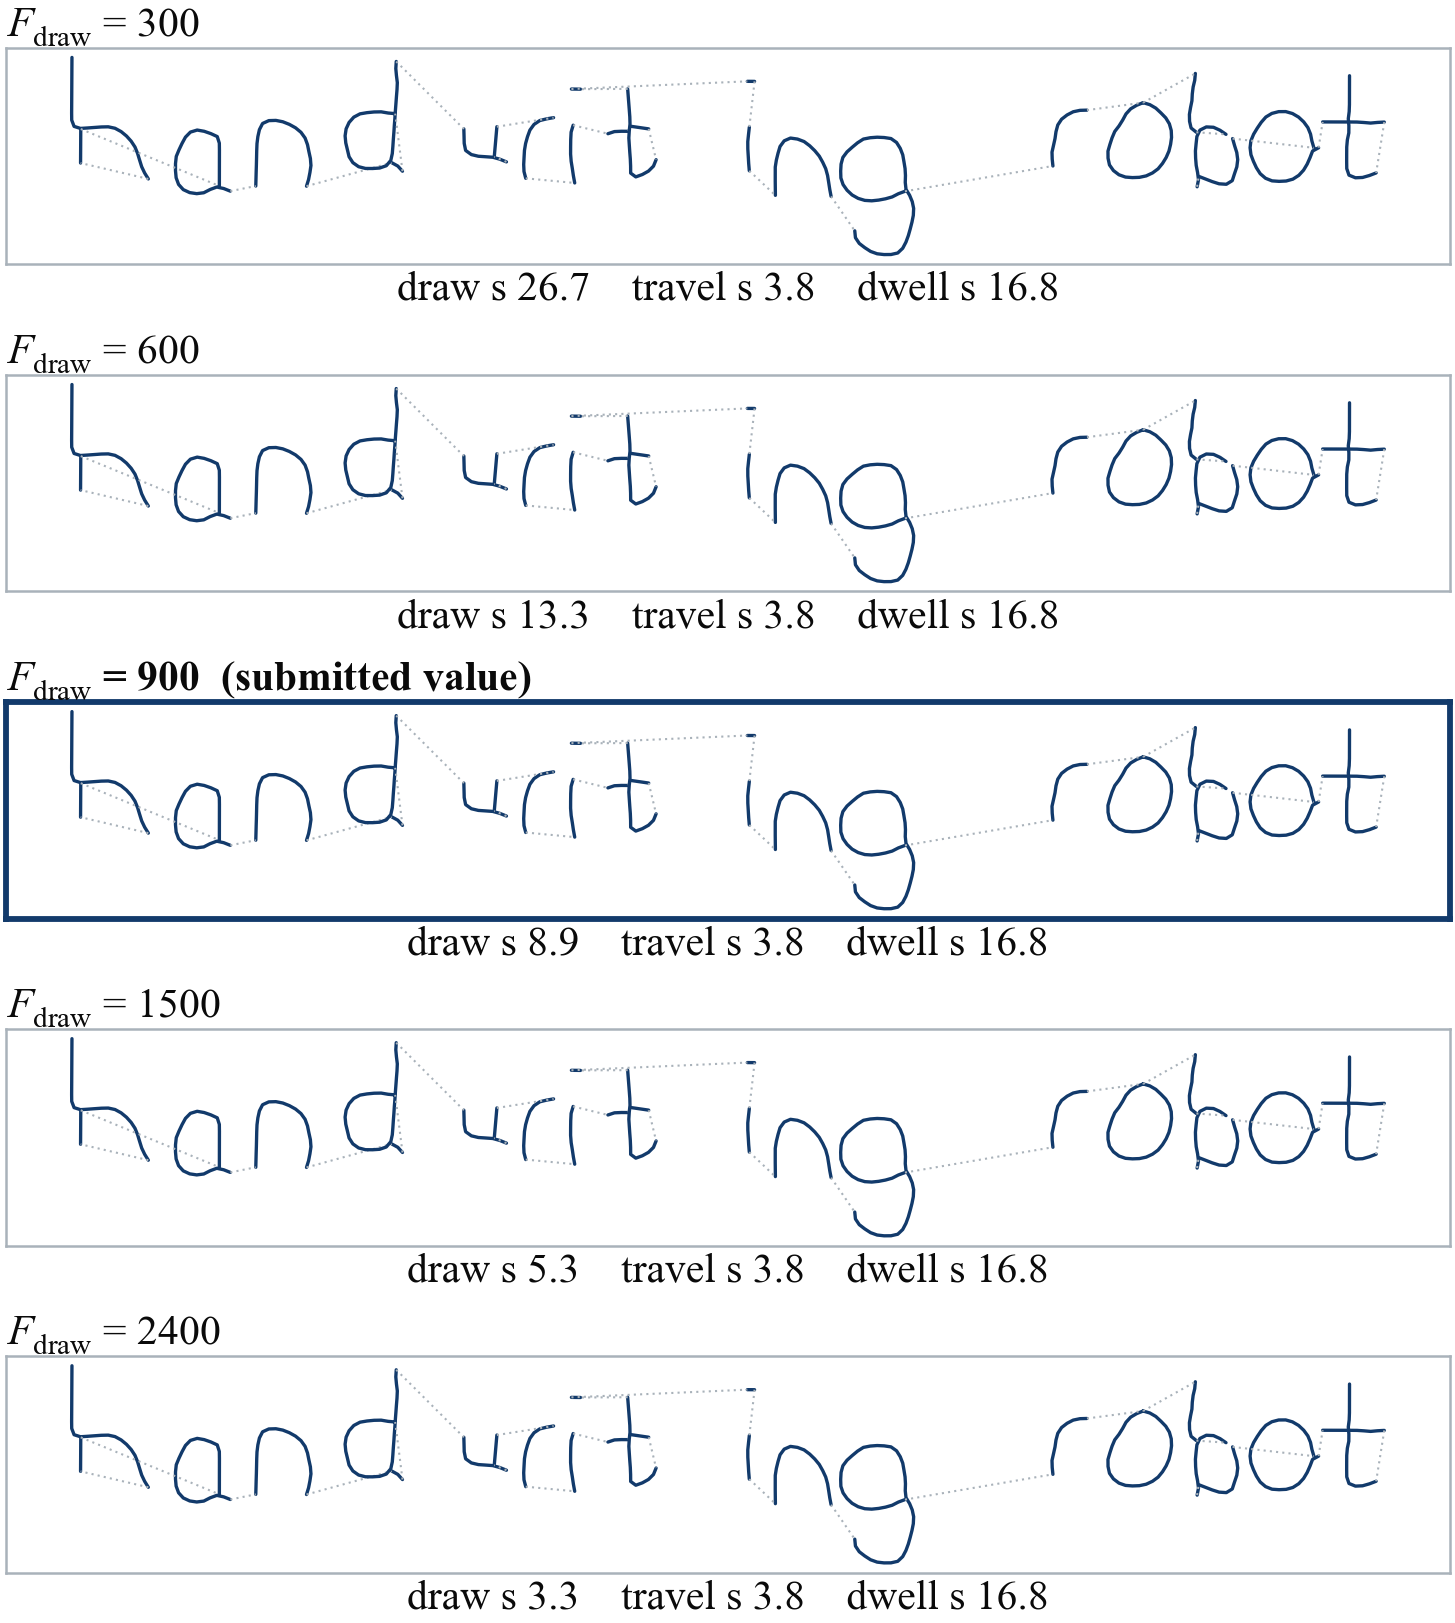
\includegraphics[width=\linewidth]{../figures/draw_feed.png}

\caption{Feed rate while drawing. Each panel is the same input processed by the submitted code with only $F_{\text{draw}}$ changed; the panel outlined in dark blue is the submitted value.}

\label{fig:draw-feed}

\end{figure}

\begin{figure}[htbp]

\centering

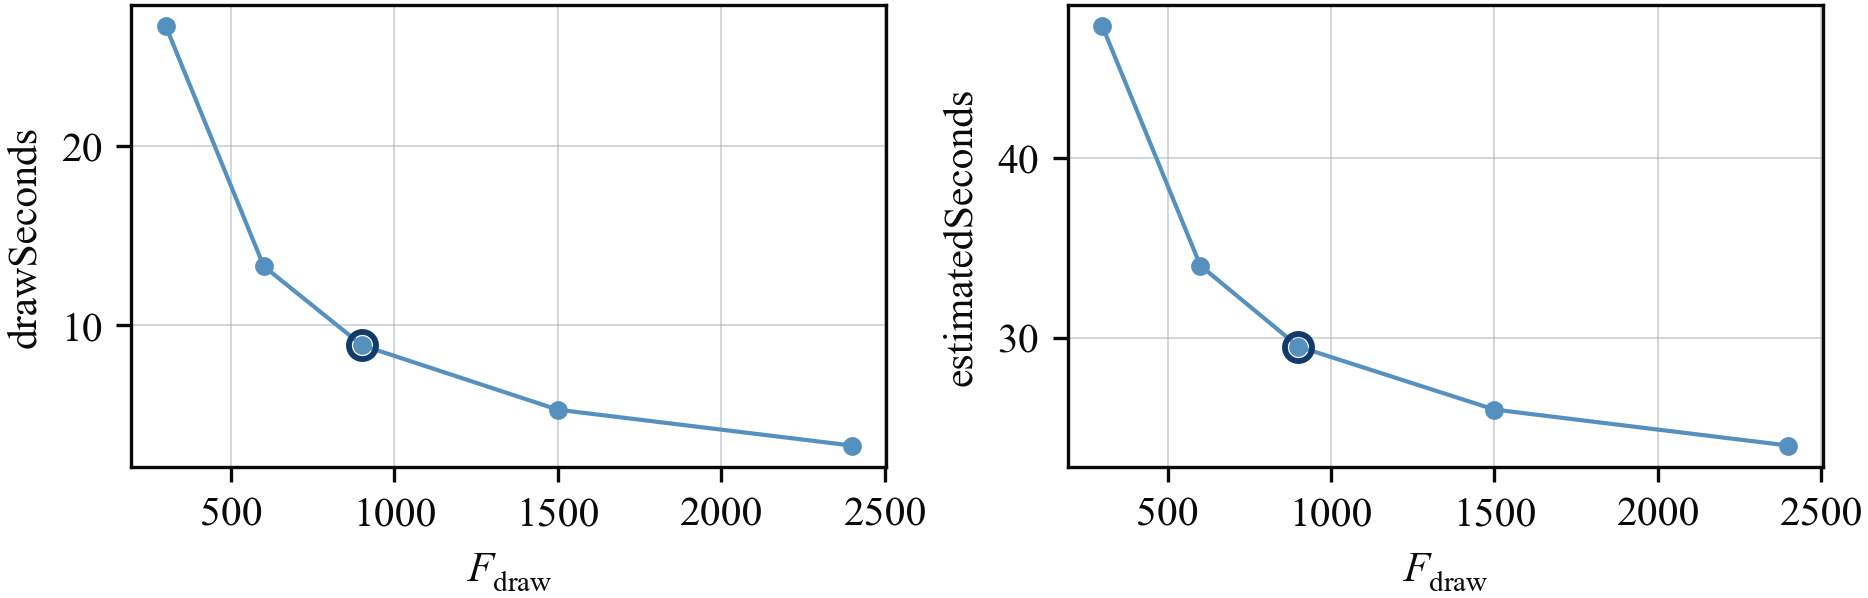
\includegraphics[width=\linewidth]{../figures/draw_feed_trend.png}

\caption{Feed rate while drawing: measured quantities against the swept value. The circled point is the submitted value.}

\end{figure}

\begin{table}[htbp]
\centering
\small
\caption{Feed rate while drawing: measured effect of each swept value. The submitted value is in bold.}
\begin{tabular}{lrrrr}
\toprule
\$F\_\{\textbackslash\{\}text\{draw\}\}\$ & \textsf{drawSeconds} & \textsf{travelSeconds} & \textsf{dwellSeconds} & \textsf{estimatedSeconds} \\
\midrule
300 & 26.7 & 3.8 & 16.8 & 47.3 \\
600 & 13.3 & 3.8 & 16.8 & 34 \\
\bfseries 900 & \bfseries 8.9 & \bfseries 3.8 & \bfseries 16.8 & \bfseries 29.5 \\
1500 & 5.3 & 3.8 & 16.8 & 26 \\
2400 & 3.3 & 3.8 & 16.8 & 24 \\
\bottomrule
\end{tabular}
\end{table}

\section{Page layout}

\subsection{X-height as a share of the ruled line spacing}

\label{coef:ruling-xh-frac}

\begin{description}[leftmargin=5.2em,style=sameline]

\item[Symbol] $f_{xh}$

\item[Value] \texttt{0.46}

\item[Source] \texttt{reproduce.py}, \texttt{GantryConfig.rulingXhFrac}

\item[Swept] \texttt{0.25}, \texttt{0.35}, \texttt{0.46}, \texttt{0.6}, \texttt{0.8}

\end{description}

\paragraph{Basis}

The ratio of x-height to line pitch is a basic typographic and palaeographic measure of a hand, and is measured per writer in the profile as \texttt{xhOverPitch}; the same ratio appears as a style feature in writer identification \cite{bulacu2007}.

\paragraph{Why this value}

The machine writes on ruled paper with an $8.4$ mm ruling, and the writing must sit on those lines at a plausible size. The x-height is therefore set as a fraction of the ruling. The fraction is only a \emph{fallback}: \texttt{XhForRuling} prefers the writer's own measured \texttt{xhOverPitch} and falls back to $f_{xh}$ only when that is missing or outside $[0.15,0.90]$. $0.46$ is close to the middle of the measured range for these writers, so the fallback produces a typical hand rather than an extreme one.

\paragraph{What the coefficient does}

Everything downstream scales with it: the pen width, the collision clearance, the drift bound and the ligature sag are all in x-heights, so changing $f_{xh}$ changes the physical size of the whole drawing and hence the drawn length and the job time. A layout that then exceeds the ruling cap \texttt{rulingMaxExtent} is shrunk again by a second pass.

\paragraph{Alternatives considered}

Setting an absolute x-height in millimetres and ignoring the ruling, which detaches the writing from the paper; or fitting the measured ascender-to-descender extent to the ruling directly, which the probe pass approximates.

\paragraph{Worked example}

At the $8.4$ mm ruling, $f_{xh} = 0.46$ gives $x_h = 3.86$ mm, and Owen's line step is $(1.51+0.68+0.85) \times 3.86 = 11.7$ mm, which exceeds one ruling, so the writing spans more than one ruled line unless the cap pulls it down.

\paragraph{What the sweep actually showed}

Run through the deployed path, where \texttt{XhForRuling} derives the x-height from the ruling, the coefficient scales the whole drawing as expected and then stops. The resulting x-heights are $2.100$, $2.940$, $3.864$, $5.040$ and $5.078$ mm, and the drawn length follows them, $69.7$, $98.1$, $129.2$, $167.4$ and $168.5$ mm, with the job estimate rising from $22.9$ to $33.5$ s. The first four are exactly $f_{xh}$ times the $8.4$ mm ruling; the fifth is not. At $f_{xh} = 0.8$ the requested x-height is $6.72$ mm, but the layout probe finds the tallest line would then exceed $\texttt{rulingMaxExtent} \times 8.4 = 10.5$ mm and scales it back to $5.078$ mm. \textbf{So this sweep also demonstrates the extent cap working}, which is the one place in the system where a requested size is overridden by a measured one, and it shows that the cap binds somewhere between $f_{xh} = 0.6$ and $0.8$ for this writer.

\begin{figure}[htbp]

\centering

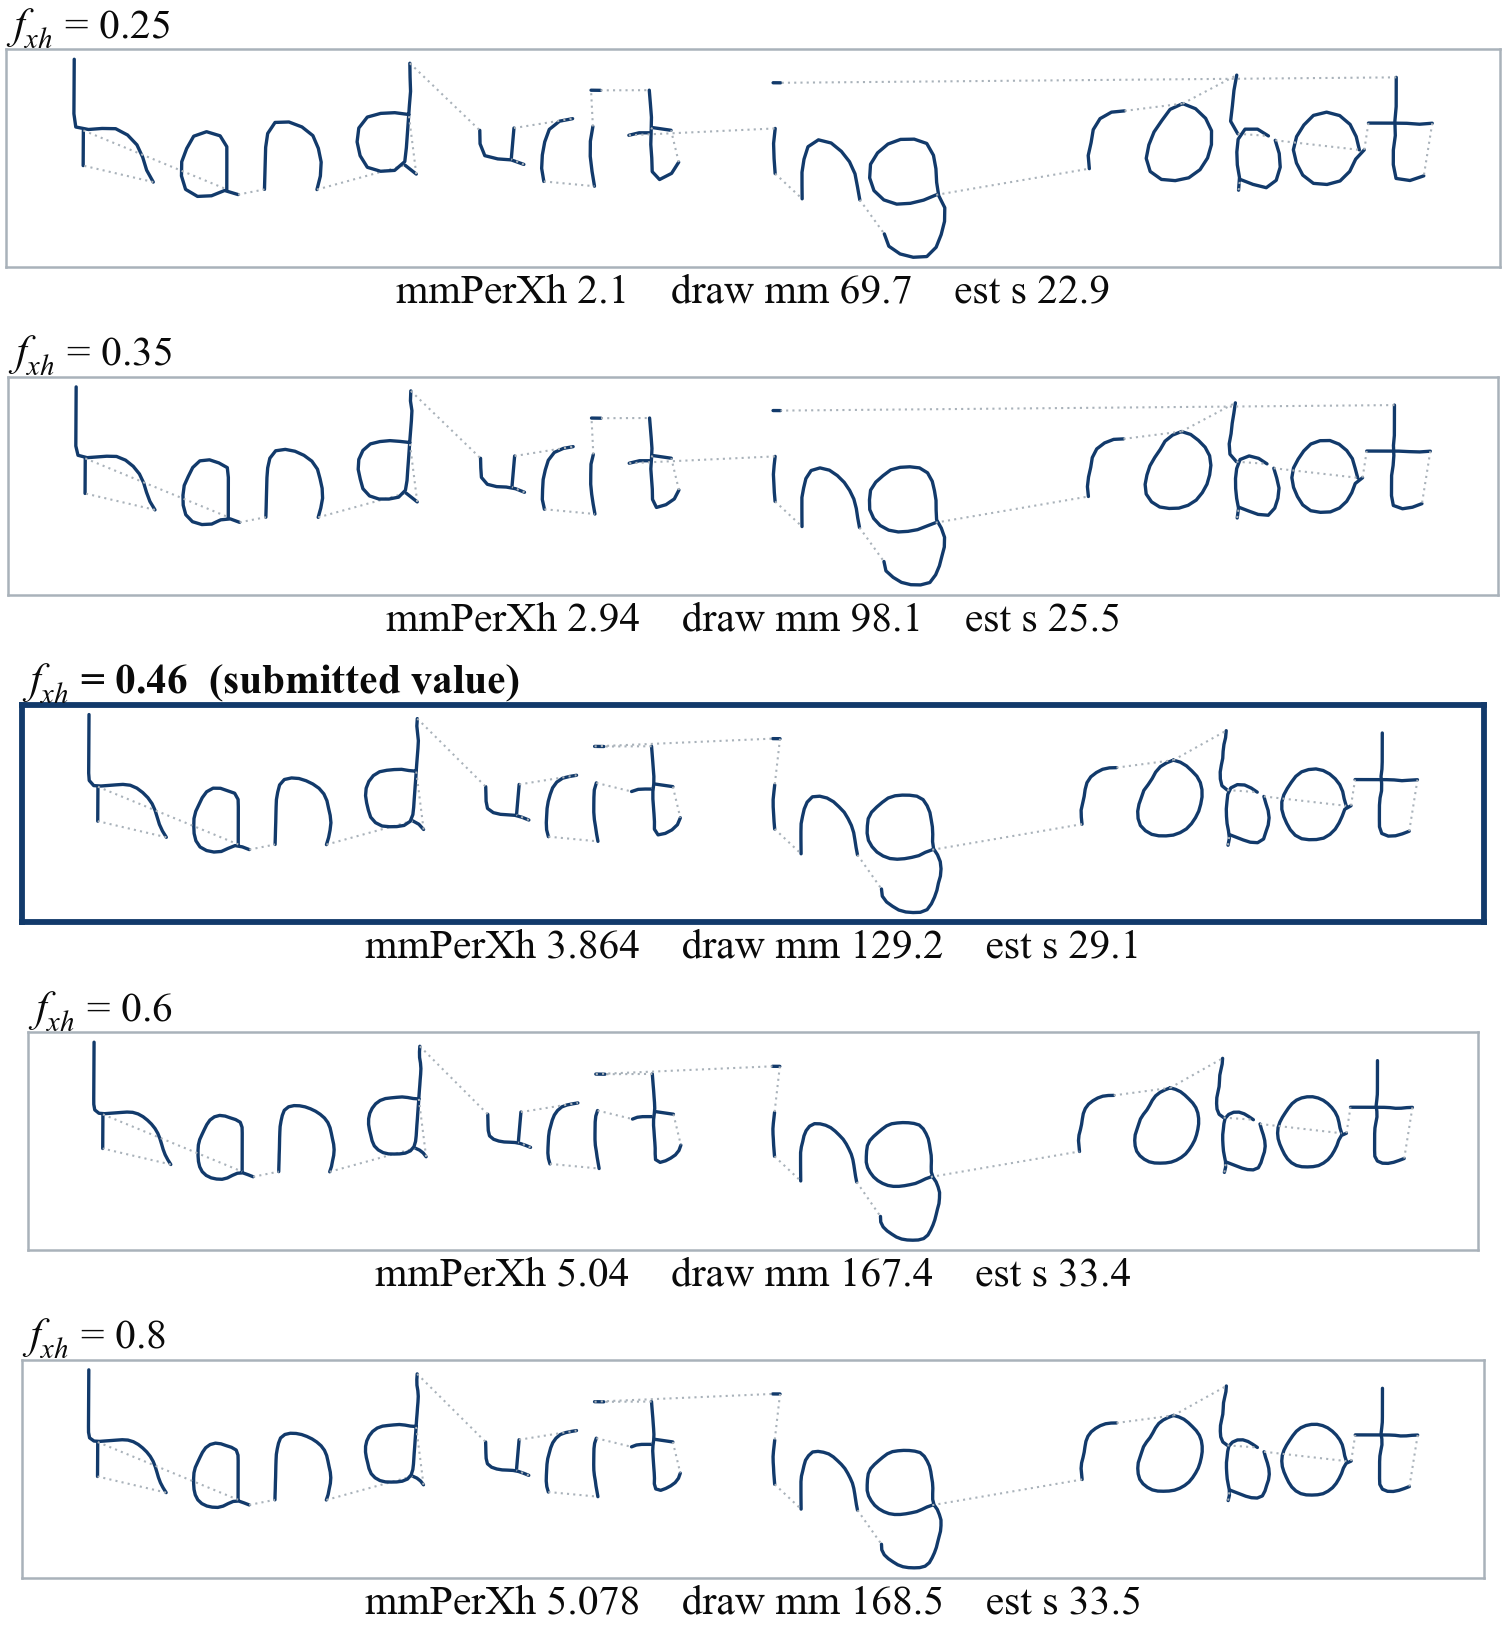
\includegraphics[width=\linewidth]{../figures/ruling_xh_frac.png}

\caption{X-height as a share of the ruled line spacing. Each panel is the same input processed by the submitted code with only $f_{xh}$ changed; the panel outlined in dark blue is the submitted value.}

\label{fig:ruling-xh-frac}

\end{figure}

\begin{figure}[htbp]

\centering

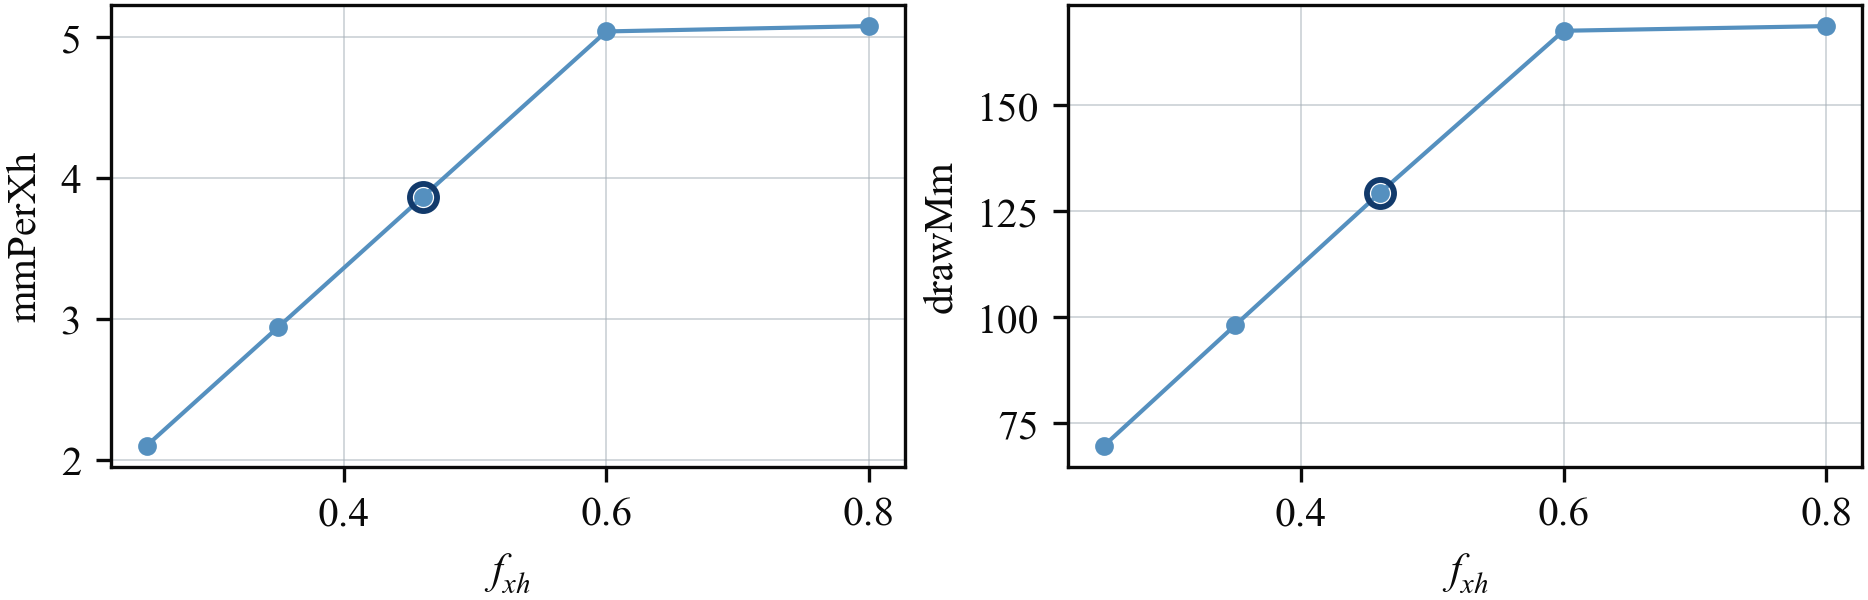
\includegraphics[width=\linewidth]{../figures/ruling_xh_frac_trend.png}

\caption{X-height as a share of the ruled line spacing: measured quantities against the swept value. The circled point is the submitted value.}

\end{figure}

\begin{table}[htbp]
\centering
\small
\caption{X-height as a share of the ruled line spacing: measured effect of each swept value. The submitted value is in bold.}
\begin{tabular}{lrrrr}
\toprule
\$f\_\{xh\}\$ & \textsf{mmPerXh} & \textsf{drawMm} & \textsf{estimatedSeconds} & \textsf{strokes} \\
\midrule
0.25 & 2.1 & 69.7 & 22.9 & 26 \\
0.35 & 2.94 & 98.1 & 25.5 & 26 \\
\bfseries 0.46 & \bfseries 3.864 & \bfseries 129.2 & \bfseries 29.1 & \bfseries 26 \\
0.6 & 5.04 & 167.4 & 33.4 & 26 \\
0.8 & 5.078 & 168.5 & 33.5 & 26 \\
\bottomrule
\end{tabular}
\end{table}

\section{End-stops}

\subsection{Interval between the samples that confirm an end-stop}

\label{coef:endstop-debounce}

\begin{description}[leftmargin=5.2em,style=sameline]

\item[Symbol] $t_{\text{db}}$

\item[Value] \texttt{0.006}

\item[Source] \texttt{reproduce.py}, \texttt{ENDSTOP\_DEBOUNCE\_S}

\item[Swept] \texttt{0.001}, \texttt{0.003}, \texttt{0.006}, \texttt{0.012}, \texttt{0.025}

\end{description}

\paragraph{Basis}

Mechanical switch contacts bounce for a period that depends on the switch; sampling until a reading is stable is the standard software debounce, and the contact-bounce behaviour of the microswitch type used is given in its data sheet \cite{stepperds}.

\paragraph{Why this value}

A limit switch on a long wire beside two stepper motors picks up both contact bounce and electrical noise. A single reading is therefore not trusted: the pin must read triggered \texttt{ENDSTOP\_CONFIRM\_SAMPLES} times in a row, $t_{\text{db}}$ apart. The interval must span a bounce so that the samples are genuinely independent, and the total confirmation time $(n-1)\,t_{\text{db}} = 12$ ms must be short against how long the carriage takes to travel the overtravel distance of the switch. At the $2400$ mm/min travel feed the carriage covers $40 \times 0.012 = 0.48$ mm in that time, which is inside the overtravel of the microswitch and well inside the $5$ mm edge tolerance.

\paragraph{What the coefficient does}

The two coefficients multiply: confirmation latency is $(n-1)\,t_{\text{db}}$ and noise rejection improves with both. A longer interval rejects longer noise bursts but lets the carriage run further past the switch before the stop takes effect. This is a safety path, so the latency is the term that must stay bounded.

\paragraph{Alternatives considered}

A hardware RC filter or a Schmitt trigger on the switch line, which removes the software cost entirely and is the better engineering answer; or an interrupt with a dead time.

\paragraph{Worked example}

$(3-1) \times 6\text{ ms} = 12$ ms of confirmation; at $40$ mm/s the carriage moves $0.48$ mm, against $5$ mm of edge tolerance, so the stop has about ten times the margin it needs.

\paragraph{Limits of this test}

\textbf{No sweep was run for this coefficient.} It can only be exercised on the gantry, with a switch, and the gantry was not run for this study. The numbers above are the arithmetic of the confirmation path, not a measurement, and the right test is to record the switch line on a scope while the carriage closes it.

\paragraph{Not swept} This coefficient was not swept; see the paragraph above for why, and what test would settle it.

\section{Seam cutting on a dense page}

\subsection{Weight on ink in the seam cost field, on a densely written page}

\label{coef:seam-ink-weight-dense}

\begin{description}[leftmargin=5.2em,style=sameline]

\item[Symbol] $w_{\text{ink}}$

\item[Value] \texttt{4.0}

\item[Source] \texttt{segment.py}, \texttt{SeamCuts}

\item[Swept] \texttt{0.5}, \texttt{1.0}, \texttt{4.0}, \texttt{16.0}, \texttt{64.0}

\end{description}

\paragraph{Basis}

Least-cost seam carving \cite[10:3]{avidan2007}, applied to handwritten line separation after \cite{arvanitopoulos2014}.

\paragraph{Why this value}

See the main entry. The point of repeating it here is that the balance between the ink term and the straightness and midline terms only matters when the seam is forced to choose between cutting through a descender and detouring a long way round it, and that choice only arises on a page where the lines are close enough to interlock.

\paragraph{What the coefficient does}

The cost of one ink pixel is $w_{\text{ink}}$ against a straightness penalty of $0.02$ per row of movement and a midline penalty reaching $0.012$. At $w_{\text{ink}} = 0.5$ one ink pixel costs the same as $25$ rows of movement, so the seam will cut through a stroke rather than detour far; at $64$ it costs $3\,200$ rows and the seam will go almost anywhere to avoid ink.

\paragraph{Alternatives considered}

A straight horizontal cut, which is what a plain profile segmenter does and which cuts every descender on a page like this one.

\paragraph{Worked example}

Abhinav's page has pitch $48$ px at half resolution against Owen's $51$, with $26$ lines against $20$, so there is roughly a quarter less clean paper between lines for the seam to use.

\paragraph{What the sweep actually showed}

The line count is $26$ and the reading accuracy $0.9939$ at every value from $0.5$ to $64$, a $128$-fold range, so by the end-to-end measure this coefficient does nothing on this page either. Comparing the seam paths themselves is far more informative, and it gives the first genuine justification for the submitted value found in this study. Taking the $w_{\text{ink}} = 64$ path as the reference and counting how many of the $1\,224$ columns of each seam sit on a different row:\begin{center}\small\begin{tabular}{rrr}\toprule$w_{\text{ink}}$ & columns differing & largest difference \\\midrule$0.5$ & $383$ & $19$ rows \\$1.0$ & $2$ & $1$ row \\$\mathbf{4.0}$ & $\mathbf{0}$ & $\mathbf{0}$ \\$16.0$ & $2$ & $1$ row \\$64.0$ & $0$ & $0$ \\\bottomrule\end{tabular}\end{center}The path converges by about $w_{\text{ink}} = 1$ and is exactly converged at the submitted $4.0$: raising the weight sixteen-fold beyond it moves the seam by nothing at all, while dropping it to $0.5$ moves $31\,\%$ of the seam, by up to $19$ rows, as it begins cutting corners through ink. The submitted value therefore sits just above the knee, with roughly a fourfold margin, and that margin costs nothing because the cost field is scale-free. On Owen's page the same comparison gives zero differing columns at \emph{every} weight from $1.0$ to $16.0$, which is why the denser page was needed to see this at all.

\paragraph{Limits of this test}

This is the same coefficient as in the entry above, run on a second, denser page. The standard probe did not exercise it: Owen's page is written at pitch $51$ with $20$ lines and the seams have clean paper to follow. Abhinav's page is cursive and carries $26$ lines at pitch $48$ on the same paper, so neighbouring lines interlock and the seam has to work.

\begin{figure}[htbp]

\centering

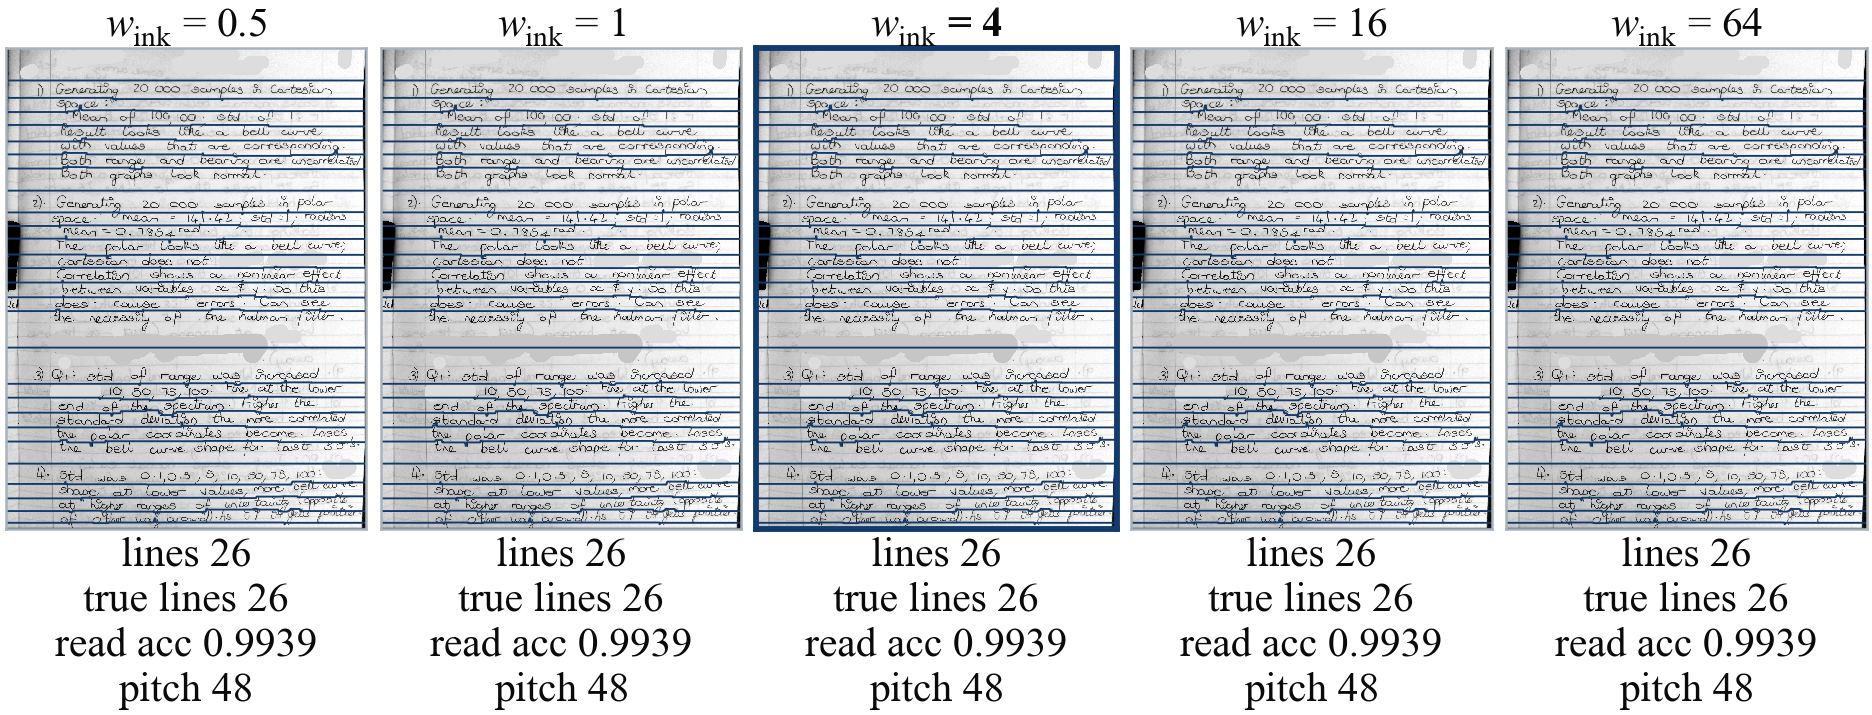
\includegraphics[width=\linewidth]{../figures/seam_ink_weight_dense.png}

\caption{Weight on ink in the seam cost field, on a densely written page. Each panel is the same input processed by the submitted code with only $w_{\text{ink}}$ changed; the panel outlined in dark blue is the submitted value.}

\label{fig:seam-ink-weight-dense}

\end{figure}

\begin{figure}[htbp]

\centering

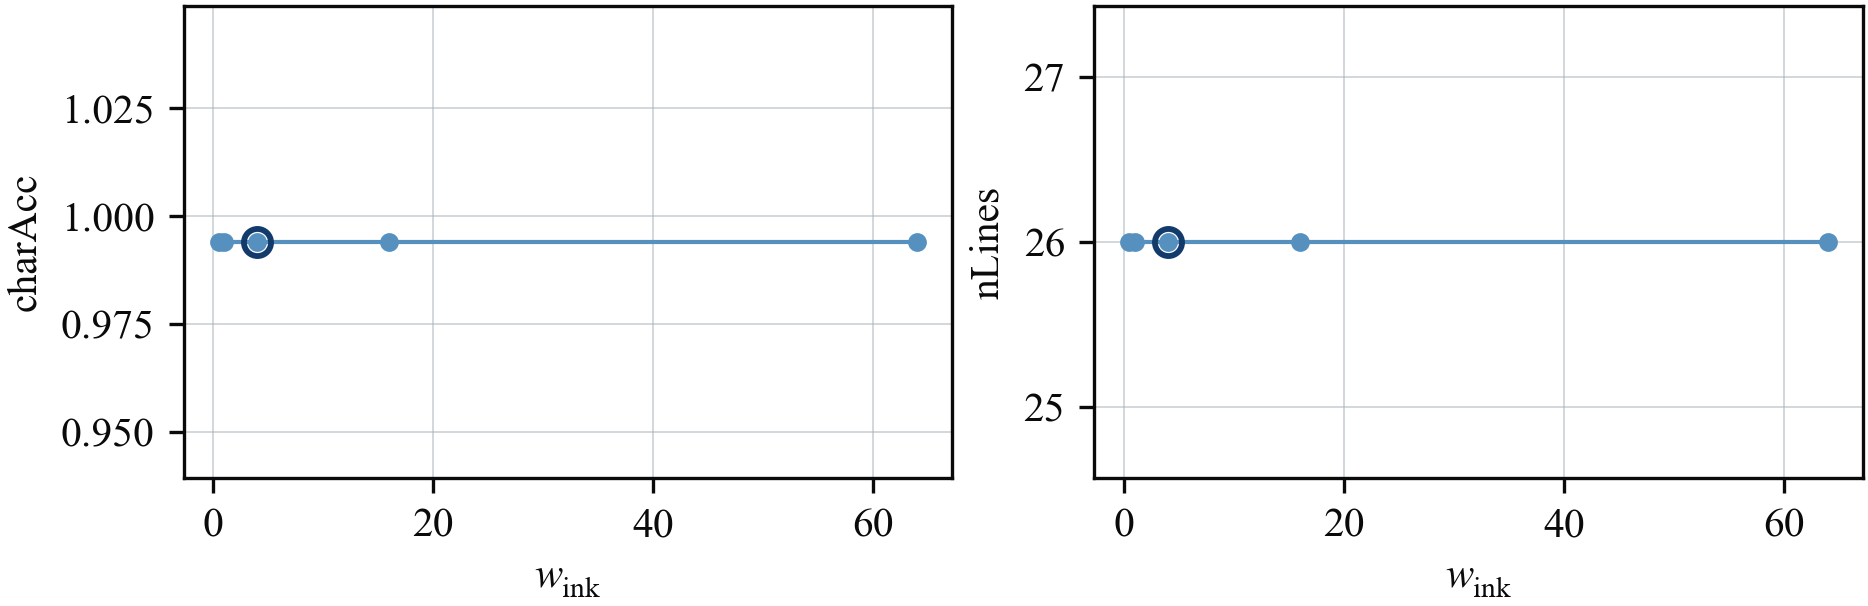
\includegraphics[width=\linewidth]{../figures/seam_ink_weight_dense_trend.png}

\caption{Weight on ink in the seam cost field, on a densely written page: measured quantities against the swept value. The circled point is the submitted value.}

\end{figure}

\begin{table}[htbp]
\centering
\small
\caption{Weight on ink in the seam cost field, on a densely written page: measured effect of each swept value. The submitted value is in bold.}
\begin{tabular}{lrrrr}
\toprule
\$w\_\{\textbackslash\{\}text\{ink\}\}\$ & \textsf{nLines} & \textsf{nLinesTruth} & \textsf{charAcc} & \textsf{pitch} \\
\midrule
0.5 & 26 & 26 & 0.9939 & 48 \\
1 & 26 & 26 & 0.9939 & 48 \\
\bfseries 4 & \bfseries 26 & \bfseries 26 & \bfseries 0.9939 & \bfseries 48 \\
16 & 26 & 26 & 0.9939 & 48 \\
64 & 26 & 26 & 0.9939 & 48 \\
\bottomrule
\end{tabular}
\end{table}

\subsection{Closing radius applied before the seam is cut, on a densely written page}

\label{coef:seam-tail-radius-dense}

\begin{description}[leftmargin=5.2em,style=sameline]

\item[Symbol] $r_{\text{tail}}$

\item[Value] \texttt{0.07}

\item[Source] \texttt{segment.py}, \texttt{SeamCuts}

\item[Swept] \texttt{0.0}, \texttt{0.03}, \texttt{0.07}, \texttt{0.16}, \texttt{0.3}

\end{description}

\paragraph{Basis}

Morphological closing before a path search \cite{haralick1987}.

\paragraph{Why this value}

See the main entry. On a dense cursive page the closing has two opposing jobs at once: it must seal the narrow channels a seam would otherwise thread through a letter, and it must not weld a descender of one line to an ascender of the next, because once they are welded no seam can pass between those two lines at all and they merge.

\paragraph{What the coefficient does}

At $P = 48$ px the radius is $\lfloor 0.07 \times 48 \rfloor = 3$ px at the submitted value and $14$ px at $0.30$. The gap between an ascender and the descender above it on this page is a few tens of pixels, so a large radius genuinely can bridge it.

\paragraph{Alternatives considered}

Sealing channels by a width test on the mask rather than a closing, which would not fatten the stroke at all.

\paragraph{Worked example}

$0.07 \times 48 = 3.36 \to 3$ px at the submitted value, against $0.07 \times 51 = 3.57 \to 3$ px on the standard probe, so the absolute radius is almost the same and only the spacing differs.

\paragraph{What the sweep actually showed}

Unlike the cost weights, the closing radius does change the outcome on a dense page, and in the predicted direction. Reading accuracy is $0.9939$ at $0$, $0.03$ and the submitted $0.07$, falls to $0.9617$ at $0.16$ and partly recovers to $0.9794$ at $0.30$. The line count stays at $26$ throughout, so this is damage to the crops rather than to the line finding: an over-large closing welds a descender to the ascender below it, the seam can no longer pass cleanly between them, and ink is handed to the wrong line. The submitted value is at the top of the flat region, which is the right place for it, though the sweep cannot separate it from $0$ or $0.03$ on this page.

\paragraph{Limits of this test}

This is the same coefficient as in the entry above, run on a second, denser page. The standard probe did not exercise it: Owen's page is written at pitch $51$ with $20$ lines and the seams have clean paper to follow. Abhinav's page is cursive and carries $26$ lines at pitch $48$ on the same paper, so neighbouring lines interlock and the seam has to work.

\begin{figure}[htbp]

\centering

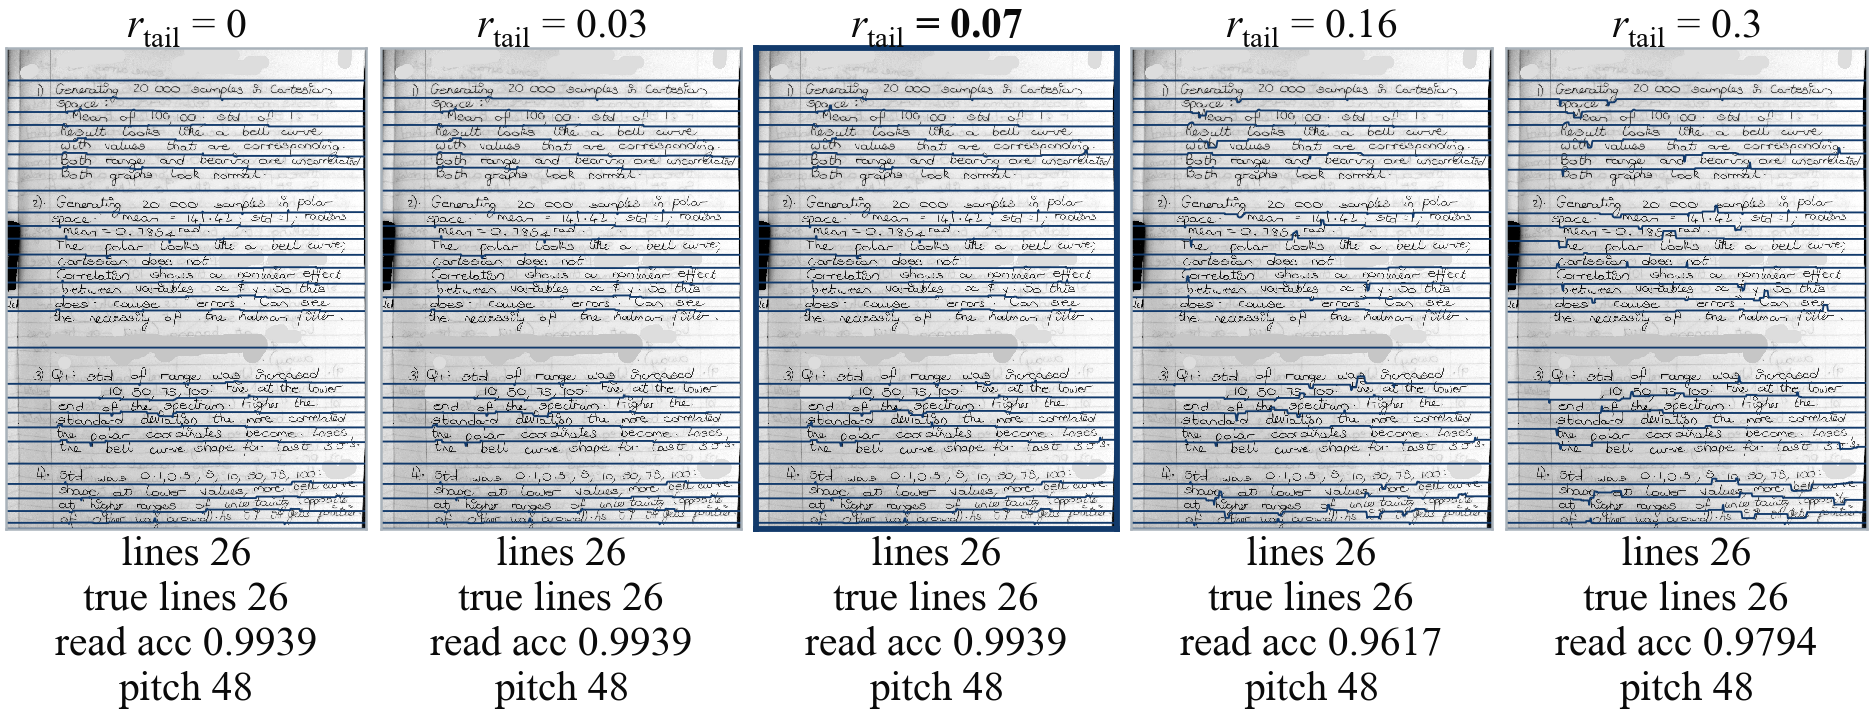
\includegraphics[width=\linewidth]{../figures/seam_tail_radius_dense.png}

\caption{Closing radius applied before the seam is cut, on a densely written page. Each panel is the same input processed by the submitted code with only $r_{\text{tail}}$ changed; the panel outlined in dark blue is the submitted value.}

\label{fig:seam-tail-radius-dense}

\end{figure}

\begin{figure}[htbp]

\centering

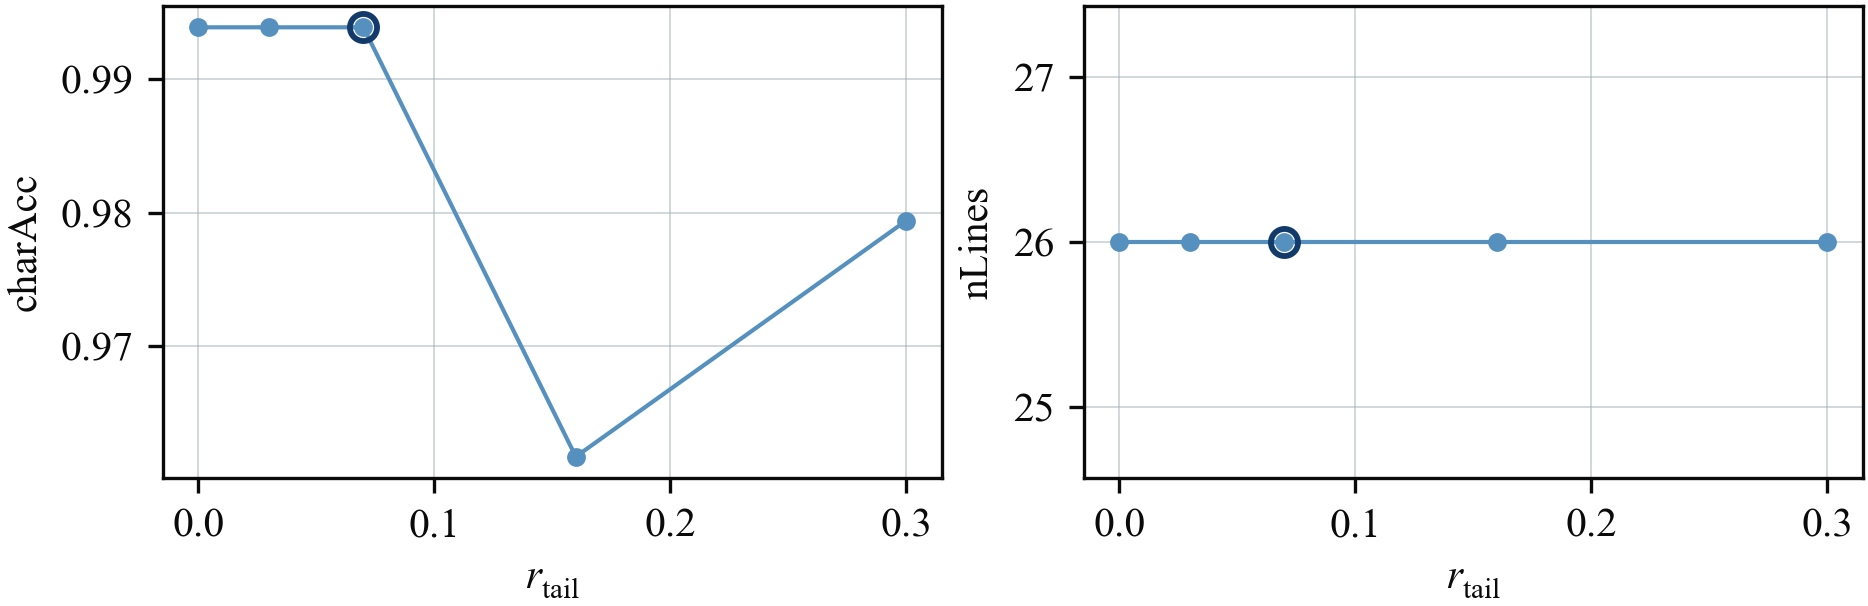
\includegraphics[width=\linewidth]{../figures/seam_tail_radius_dense_trend.png}

\caption{Closing radius applied before the seam is cut, on a densely written page: measured quantities against the swept value. The circled point is the submitted value.}

\end{figure}

\begin{table}[htbp]
\centering
\small
\caption{Closing radius applied before the seam is cut, on a densely written page: measured effect of each swept value. The submitted value is in bold.}
\begin{tabular}{lrrrr}
\toprule
\$r\_\{\textbackslash\{\}text\{tail\}\}\$ & \textsf{nLines} & \textsf{nLinesTruth} & \textsf{charAcc} & \textsf{pitch} \\
\midrule
0 & 26 & 26 & 0.9939 & 48 \\
0.03 & 26 & 26 & 0.9939 & 48 \\
\bfseries 0.07 & \bfseries 26 & \bfseries 26 & \bfseries 0.9939 & \bfseries 48 \\
0.16 & 26 & 26 & 0.9617 & 48 \\
0.3 & 26 & 26 & 0.9794 & 48 \\
\bottomrule
\end{tabular}
\end{table}

\subsection{Share of a piece's ink that must lie in a band, on a densely written page}

\label{coef:band-ink-share-dense}

\begin{description}[leftmargin=5.2em,style=sameline]

\item[Symbol] $\theta_{\text{band}}$

\item[Value] \texttt{0.15}

\item[Source] \texttt{segment.py}, \texttt{\_BandOwnership}

\item[Swept] \texttt{0.02}, \texttt{0.08}, \texttt{0.15}, \texttt{0.3}, \texttt{0.5}

\end{description}

\paragraph{Basis}

Component-to-line assignment after a coarse cut \cite{likforman2007}.

\paragraph{Why this value}

See the main entry. Ownership only becomes contentious when a piece of ink genuinely spans two bands, which on a well-spaced page is rare and on a dense cursive page is common: a descender from one line routinely reaches into the body of the next.

\paragraph{What the coefficient does}

Because a piece substantial in more than one band is given to the topmost, lowering $\theta_{\text{band}}$ pulls ink upward and raising it falls back on majority ownership, which hands a long descender to the line below the one it was written on.

\paragraph{Alternatives considered}

Majority ownership alone, or assignment by centroid.

\paragraph{Worked example}

A piece with $300$ ink pixels counts as present in a band at $45$ pixels at the submitted value, $6$ pixels at $0.02$ and $150$ at $0.50$.

\paragraph{What the sweep actually showed}

The denser page does expose an effect, but only at the top of the range: $26$ lines and $0.9939$ accuracy at $0.02$, $0.08$, the submitted $0.15$ and $0.30$, falling to $0.9893$ at $0.50$. At that setting a piece must put half its ink in a band to count as present there, so a descender reaching into the line below no longer registers in both, the topmost-band rule stops applying to it, and it is assigned by majority to the wrong line. The submitted value sits inside a wide flat region that extends well below it, so the sweep confirms the value is safe without distinguishing it from $0.02$; the argument for $0.15$ rather than $0.02$ remains the one given above, that a few pixels of anti-aliased overlap should not count as presence.

\paragraph{Limits of this test}

This is the same coefficient as in the entry above, run on a second, denser page. The standard probe did not exercise it: Owen's page is written at pitch $51$ with $20$ lines and the seams have clean paper to follow. Abhinav's page is cursive and carries $26$ lines at pitch $48$ on the same paper, so neighbouring lines interlock and the seam has to work.

\begin{figure}[htbp]

\centering

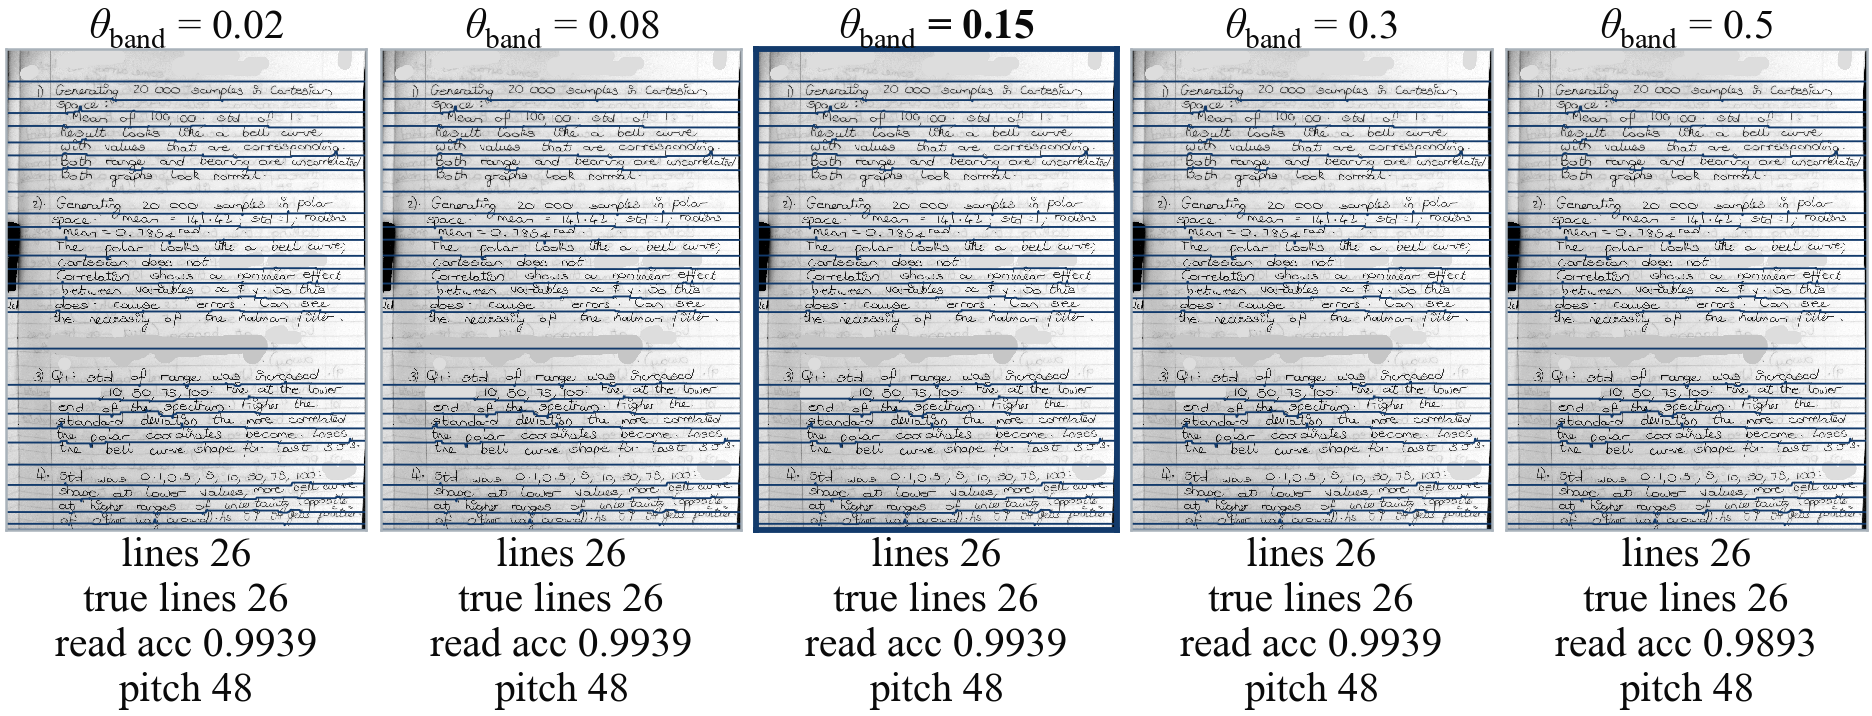
\includegraphics[width=\linewidth]{../figures/band_ink_share_dense.png}

\caption{Share of a piece's ink that must lie in a band, on a densely written page. Each panel is the same input processed by the submitted code with only $\theta_{\text{band}}$ changed; the panel outlined in dark blue is the submitted value.}

\label{fig:band-ink-share-dense}

\end{figure}

\begin{figure}[htbp]

\centering

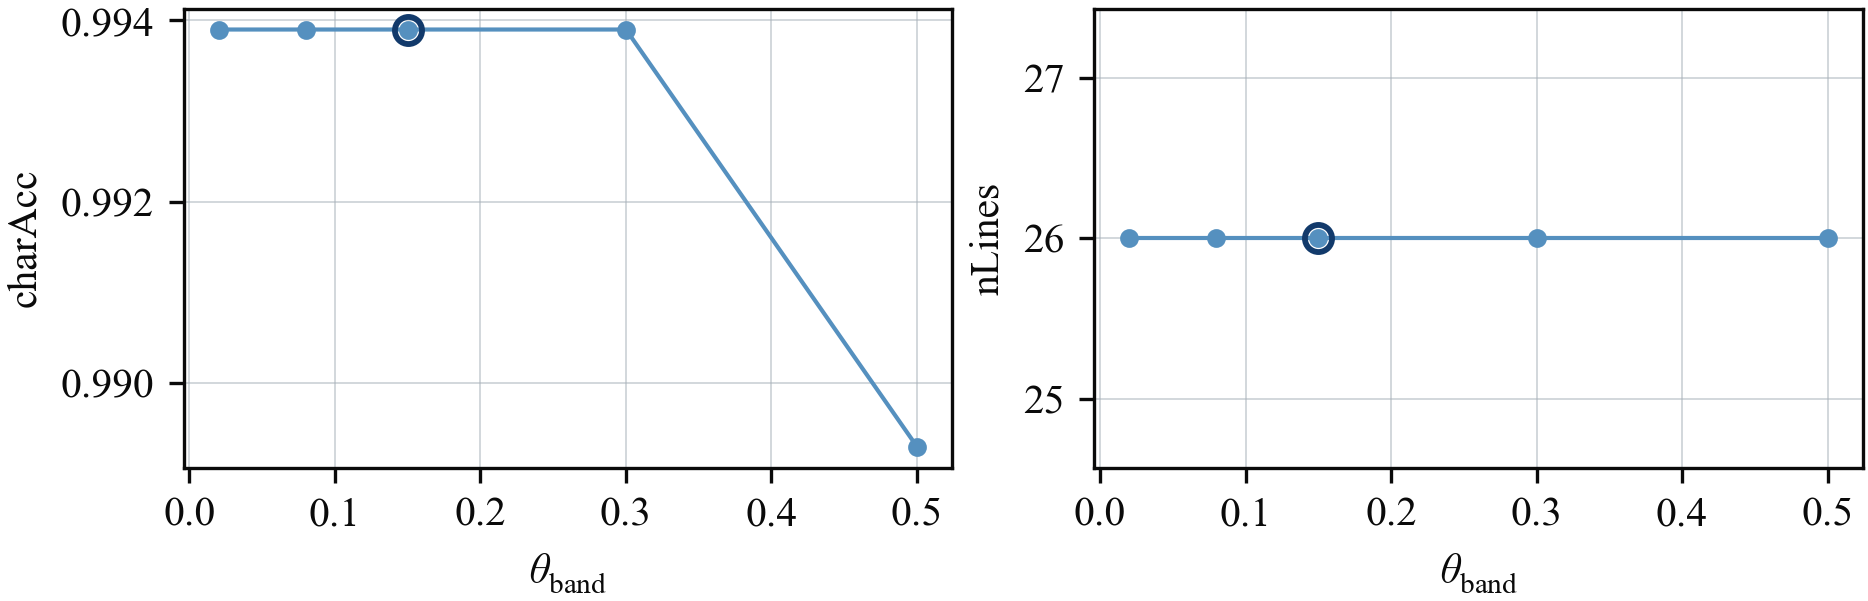
\includegraphics[width=\linewidth]{../figures/band_ink_share_dense_trend.png}

\caption{Share of a piece's ink that must lie in a band, on a densely written page: measured quantities against the swept value. The circled point is the submitted value.}

\end{figure}

\begin{table}[htbp]
\centering
\small
\caption{Share of a piece's ink that must lie in a band, on a densely written page: measured effect of each swept value. The submitted value is in bold.}
\begin{tabular}{lrrrr}
\toprule
\$\textbackslash\{\}theta\_\{\textbackslash\{\}text\{band\}\}\$ & \textsf{nLines} & \textsf{nLinesTruth} & \textsf{charAcc} & \textsf{pitch} \\
\midrule
0.02 & 26 & 26 & 0.9939 & 48 \\
0.08 & 26 & 26 & 0.9939 & 48 \\
\bfseries 0.15 & \bfseries 26 & \bfseries 26 & \bfseries 0.9939 & \bfseries 48 \\
0.3 & 26 & 26 & 0.9939 & 48 \\
0.5 & 26 & 26 & 0.9893 & 48 \\
\bottomrule
\end{tabular}
\end{table}

\clearpage
\section{Choices that cannot honestly be swept}
\label{sec:arch}

The constants in this section define the trained networks. Changing any of them
and re-running the pipeline does not measure the choice: it measures a
mismatch between the new shape and weights that were fitted under the old one.
Answering \enquote{why this value} for these requires either a published basis
or a retraining run, and retraining was not done for this study. They are
therefore explained, with the arithmetic that constrains them, and the sweep is
honestly declined.

\subsection{The shared convolutional backbone}

Both networks begin with the same backbone: three stages of
$3\times3$ convolutions with padding~1, each convolution followed by batch
normalisation and a ReLU, with a $2\times2$ max pool after the first and second
stages.

\begin{table}[htbp]
\centering
\caption{The shared backbone. Parameter counts include batch-norm scale, shift
and running statistics.}
\begin{tabular}{llrrr}
\toprule
\textsf{stage} & \textsf{layers} & \textsf{in} & \textsf{out} & \textsf{parameters} \\
\midrule
\texttt{stage1} & 2 & 1 & 32 & 9\,824 \\
\texttt{stage2} & 4 & 32 & 64 & 130\,304 \\
\texttt{stage3} & 6 & 64 & 128 & 814\,848 \\
\midrule
total & \ArchConvLayers & & & \ArchBackboneParams \\
\bottomrule
\end{tabular}
\end{table}

\paragraph{Why $3\times3$ convolutions stacked, rather than larger kernels.}
Two stacked $3\times3$ layers see the same $5\times5$ region as one $5\times5$
layer, with fewer parameters and an extra non-linearity between them. The CRNN
architecture this reader follows uses exactly this arrangement
\cite[p.~2298]{shi2017}. The derived receptive field of the whole backbone is
\textbf{\ArchRF{} pixels} at a stride of \ArchStride, so one output column
summarises a $72$-pixel-wide window of the $64\times640$ canvas, which at the
measured probe scale is about three x-heights: wide enough to see a character
and its neighbours, narrow enough that a column is not dominated by a whole
word.

\paragraph{Why channels widen 32, 64, 128 while the resolution falls.}
This is the standard pyramid: each pooling halves the spatial extent, and the
channel count is doubled to keep the representational capacity roughly constant
while the features become more abstract \cite{lecun1998,shi2017}.

\paragraph{Why only two pooling stages, and never on the width again.}
This is the hard constraint of the whole reader and it is arithmetic, not taste.
CTC needs at least as many input columns as output symbols, and strictly more
where a character repeats, because a blank must separate the repeat
\cite[pp.~370--372]{graves2006}. The canvas is $640$ wide and the width is
pooled twice, so the reader produces $T = 640/4 = \ArchFrames{}$ columns. The
code records the resulting safe label length as
$\lfloor \ArchFrames \times 0.75 \rfloor = \ArchMaxLabel{}$ characters. A third
pooling stage would halve $T$ to $80$ and the safe label length to $60$
characters, which is shorter than ordinary lines on these pages, and those lines
would become untrainable. That is why stage~3 has six convolution layers and no
pool: depth is bought without spending resolution.

\paragraph{Why the height is collapsed by an adaptive max, not flattened.}
After stage~3 the feature map is pooled to a single row by taking the maximum
over height. Flattening instead would make the number of features depend on the
input height and tie the network to one canvas size; taking the maximum keeps
the strongest response per column per channel and makes the backbone
height-agnostic, which is what lets the same backbone serve the writer
classifier unchanged.

\paragraph{Batch normalisation.} Applied after every convolution with the usual
momentum $0.1$ and $\epsilon = 10^{-5}$ \cite[Alg.~1]{ioffe2015}. At inference
the running mean and variance are folded into a single scale and shift, which is
what \texttt{recognise.py} does.

\paragraph{ReLU.} $\max(0,x)$ \cite[p.~807]{nair2010}, chosen for the same
reason it is used everywhere: it does not saturate for positive inputs, so
gradients reach the early layers of a twelve-layer stack.

\subsection{The reader's recurrent stack and head}

The $128$ channels per column are read by two bidirectional LSTM layers of
$256$ units per direction, and a linear layer maps the resulting $512$ features
to \ArchClasses{} classes: the $74$ characters of the charset plus the CTC
blank in slot~0.

\begin{description}[leftmargin=2em]
\item[The LSTM cell] is Hochreiter and Schmidhuber's \cite{hochreiter1997};
the input, forget, cell and output gates are computed in one matrix product and
split, which is why the stored gate matrices have $4n_h$ rows.
\item[Reading both directions] is Schuster and Paliwal's \cite{schuster1997}:
a character's identity depends on what follows it as well as what precedes it,
and a unidirectional pass cannot use the right context.
\item[Two layers of 256] is the size used by the CRNN this follows
\cite[p.~2298]{shi2017} and by the handwriting system of Graves \textit{et al.}
\cite[p.~855]{graves2009}. The recurrent stack holds \ArchLstmParams{}
parameters, which is $70\,\%$ of the reader's \ArchReaderTotal{} total: it, not
the backbone, is where the reader's capacity sits, and it is also what dominates
inference time on the ODROID, since the recurrence is sequential over
\ArchFrames{} columns.
\item[CTC] \cite[pp.~370--372]{graves2006} removes the need for per-character
alignment in the training labels, which matters here because the transcripts are
typed line by line with no character positions. The same forward--backward
machinery, run in forced-alignment mode, is what later supplies the character
boundaries the glyph cutter uses.
\end{description}

\paragraph{Why this cannot be swept.} The checkpoint stores gate matrices of
shape $4n_h \times n_{\text{in}}$ and $4n_h \times n_h$. Changing $n_h$ makes
those shapes inconsistent with the stored arrays and the forward pass raises.
The sweep in section~\ref{coef:lstm-hidden} is included precisely so that this
is on the record.

\subsection{The writer classifier's head, and dropout}

The writer classifier uses the same backbone, pools over height \emph{and} then
over width, and passes the resulting $128$ features through a $96$-unit ReLU
layer, dropout at $p = 0.2$, and a linear layer to one score per writer. The
head holds $13\,645$ parameters against the backbone's \ArchBackboneParams{},
so the classifier is almost entirely shared backbone.

\paragraph{Why pool over width as well.} Writing style is a property of the
whole line, not of a position in it. Averaging over width makes the descriptor
order-free, so the classifier cannot identify a writer by \emph{which} words
they wrote --- which matters because each writer copied a different passage, and
a width-sensitive model could learn the passage instead of the hand.

\paragraph{Why dropout $0.2$ and not the customary $0.5$.} Dropout
\cite[p.~1930]{srivastava2014} is applied at one place only: the $96$-unit
hidden layer of the head. The convolutional backbone has no dropout, because
batch normalisation is already regularising it and dropout between convolutions
interacts badly with batch-norm statistics. On a $96$-unit layer, $p = 0.5$
leaves $48$ effective units feeding a $13$-way decision, which is a severe
bottleneck for a head this small; $p = 0.2$ leaves about $77$. The customary
$0.5$ in \cite{srivastava2014} is quoted for much wider fully connected layers.

\paragraph{Why this is not swept.} Dropout is inactive at inference --- the
submitted \texttt{recognise.py} notes this at the point where the head is
evaluated --- so sweeping it without retraining would change nothing at all and
produce five identical panels. Measuring it honestly means retraining the
classifier at each value, which was not done.

\subsection{Initialisation, optimisers and schedules}

\begin{description}[leftmargin=2em]
\item[Convolution initialisation] is Kaiming normal,
$\sigma = \sqrt{2/\text{fan-in}}$ \cite{he2015}, whose gain of $2$ is derived
for exactly the ReLU non-linearity used here.
\item[Linear and LSTM initialisation] is uniform on
$\pm 1/\sqrt{\text{fan-in}}$, the convention these layers are normally built
with.
\item[The reader] is trained with RMSprop \cite[Lec.~6e]{tieleman2012},
$\alpha = 0.99$, weight decay $10^{-5}$, and the learning rate is halved after
five epochs without improvement, floored at $10^{-5}$.
\item[The writer classifier] is trained with AdamW
\cite[Alg.~2]{loshchilov2019}, weight decay $10^{-4}$ applied separately from
the gradient step, on a cosine schedule \cite{loshchilov2017} over the run.
\item[Gradient clipping] at a global norm of $5.0$ \cite[Alg.~1]{pascanu2013}
guards the recurrent stack, where long sequences make exploding gradients a real
risk.
\end{description}

The two tasks use different optimisers because they are different problems: the
CTC loss over \ArchFrames{} columns is noisy and benefits from RMSprop's
per-parameter scaling without momentum, while the classifier is a small,
well-posed cross-entropy problem where AdamW with decoupled weight decay and a
cosine schedule converges in a fixed epoch budget.

\subsection{Augmentation}

Four augmentations are available: shear by $\pm 0.6$ in $\tan$, which is
$\pm 31^\circ$; rotation by $\pm 2.5^\circ$; a perspective warp with corner
displacement $3$--$8\,\%$ of the half-dimension; and an elastic deformation with
$\sigma \in \{3,4\}$ and $\alpha \in \{15,20\}$, after Simard \textit{et al.}
\cite{simard2003}. They model the real variation in the input: a page is
photographed from a slightly wrong angle (perspective), held at a slight tilt
(rotation), and written with a varying lean (shear).

The selection rule is worth stating exactly, because it is easy to misread.
Each of the four is made a candidate independently with probability $0.5$, and
then \emph{one} candidate is chosen at random. The marginal probability that a
given augmentation is applied is therefore not $0.5$ but
$\ArchPEachAug\,\%$, and a crop passes through unaugmented
$\ArchPNoAug\,\%$ of the time.

\subsection{The held-out split and the personal fraction}

\texttt{paths.py} fixes \texttt{ValFraction = 0.15} and
\texttt{SplitSeed = 0}, shared by every script so that a line held out for one
model is held out for the other. The seed is fixed so the split is reproducible
across machines and across reruns; the fraction trades training material
against the precision of the held-out estimate. At $15\,\%$ of $1\,000$ lines
the validation set is $150$ lines, and a $90\,\%$ accuracy measured on it
carries a Wilson $95\,\%$ interval \cite{wilson1927} of roughly $\pm 4.7$
percentage points. Raising the fraction narrows that interval as
$1/\sqrt{n}$ while taking lines away from training; the recorded arithmetic over
a range of set sizes is in \texttt{results/architecture.json}.

\texttt{train.py} takes \texttt{--personal-fraction} with a default of $0.20$.
The reader is trained on a public corpus plus the five photographed writers, and
the photographed set is far smaller. Without forcing, a batch would rarely
contain a photographed line and the reader would never adapt to the pages the
robot actually has to read. \texttt{IterateMixedBatches} therefore draws a fixed
proportion from each set, reusing the smaller set as often as needed. At the
default and a batch of~8 that is exactly $2$ photographed lines and $6$ public
lines in every batch.

\section{What is covered and what is not}

\subsection{Covered}

Every coefficient listed in section~\ref{sec:summary} is documented with a
basis, a reason, an explanation, alternatives and a worked example. Those marked
with a run count are swept with a figure.

\subsection{Not covered, and why}

\begin{description}[leftmargin=2em]
\item[Anything requiring retraining] The network shapes, the dropout rate, the
optimiser settings, the augmentation ranges, the validation fraction and the
personal fraction all need a training run per value to be measured. They are
explained in section~\ref{sec:arch} and not swept.
\item[Anything requiring the gantry] The end-stop debounce and confirmation
count, the homing step delay, the retract distance, the pen-up overrun and the
measured switch travel can only be exercised on the machine. The pen dwell is
swept \emph{as arithmetic on the generated job}, which is honest about job time
but says nothing about whether the nib seats.
\item[The old segmentation comparison] Running the earlier segmentation to show
its effect on classification accuracy is a separate experiment against a
different code base, not a coefficient sweep, and it is not in this document.
\end{description}

\section{Running a sweep live}
\label{sec:demo}

The study is driven from
\path{Report/CoefficientJustification_2026-11-10/sweep}.

\begin{description}[leftmargin=2em]
\item[List every coefficient] \texttt{python run.py -{}-list}
\item[Sweep one coefficient] \texttt{python run.py darkness\_gamma}
\item[Sweep everything] \texttt{python run.py}
\item[Check the patch targets] \texttt{python validate.py}
\end{description}

To demonstrate a different value during the demonstration, edit the
\texttt{values} list of that coefficient in the matching
\texttt{sweep/coeffs\_*.py} file and re-run the one key. The figure in
\texttt{figures/} and the record in \texttt{results/} are both rewritten, and
the submitted code is verified unchanged at the end of every run.

Nothing in \path{Software/u23539195_BrauneDR_Code} is ever written to. A
sweep builds its own copy of the seven modules in a scratch directory, rewrites
one token in it, and runs that. The copy also has its data path rewritten to an
absolute path, because it no longer sits beside the data folder; that is the
only other change made to any copy.

\clearpage
\bibliographystyle{ieeetr}
\bibliography{references}

\end{document}
